\documentclass[master=cws,masteroption=gs]{config/kulemt}
\setup{title={Multi-tenant performance SLOs for container orchestrated batch workloads},
  author={Matthijs Kaminski},
  promotor={Prof.\,dr.\,ir.\ Wouter Joosen \and  Dr. Eddy Truyen},
  assessor={Prof.\,dr.\ Adalberto Simeone \and Emad Heydari Beni},
  assistant={Emad Heydari Beni}}
% The following \setup may be removed entirely if no filing card is wanted
\setup{filingcard,
  translatedtitle=,
  udc=681.3,
  shortabstract={  SaaS Providers face the constant challenge to maximize the use of their rented infrastructure in order to offer their software service at the most competitive price. Often a multi-tenant architecture is employed in order to maximize resource sharing between tenants. This requires techniques to differentiate the service between different classes of tenants. The quality of the service provided is specified in an Service Level Agreement (SLA) between tenant and provider. Recent work states that the resource management concepts of container technology such as Docker and  container orchestration platforms such as Kubernetes can be used to achieve multi-tenancy with quality of service differentiation while offering fine-grained resource allocation. In order to use these container orchestration concepts, SaaS providers need to translate Service Level Objectives (SLOs), which are part of the SLA, to low-level resource allocations. This difficult task typically requires extensive domain expertise.Existing state-of-the-art approaches to this problem rely on a model of the application and therefore again requires extensive domain expertise in order to create an accurate model of the application. In opposition to this approach, we propose a generic  approach that does not require any model of the application or another type of domain expertise. Instead, we determine mappings between SLOs and resource allocations by adapting a performance tuning technique that relies on continuous experimentation of the application in the production environment. We believe such continuous experimentation is feasible in contemporary DevOps environments where a new version of the application is tested in the production environment before exposing it to clients.In this master thesis this approach is implemented as part of an automated tool, k8-resource-optimizer,  capable of translating SLOs for a given application and workload to Kubernetes resource concepts.  Experimental evaluation of k8-resource-optimizer with a simple batch processing application has shown that this approach is practically able to produce an optimal or near-optimal resource allocation in various deployment scenarios with one or more SLOs for one or more tenant organizations. Therefore,  k8-resource-optimizer shows potential as a useful DevOps tool.}}
% Uncomment the next line for generating the cover page
% \setup{coverpageonly}
% Uncomment the next \setup to generate only the first pages (e.g., if you
% are a Word user.
%\setup{frontpagesonly}

% Choose the main text font (e.g., Latin Modern)
\setup{font=lm}

% If you want to include other LaTeX packages, do it here. 

% Finally the hyperref package is used for pdf files.
% This can be commented out for printed versions.
\usepackage[pdfusetitle,colorlinks,plainpages=false]{hyperref}

%%%%%%%
% The lipsum package is used to generate random text.
% You never need this in a real master's thesis text!
\IfFileExists{lipsum.sty}%
 {\usepackage{lipsum}\setlipsumdefault{11-13}}%
 {\newcommand{\lipsum}[1][11-13]{\par And some text: lipsum ##1.\par}}
%%%%%%%




\usepackage{amsmath}
\usepackage{float}
\usepackage{csquotes}
\usepackage{subfigure}
\usepackage{graphicx}
\usepackage{caption}
\usepackage{subcaption}

% Code for YAML highlighting
\usepackage[dvipsnames]{xcolor}
\usepackage{listings}

\newcommand\YAMLcolonstyle{\color{red}\mdseries}
\newcommand\YAMLkeystyle{\color{black}\bfseries}
\newcommand\YAMLvaluestyle{\color{blue}\mdseries}

\makeatletter

% here is a macro expanding to the name of the language
% (handy if you decide to change it further down the road)
\newcommand\language@yaml{yaml}

\expandafter\expandafter\expandafter\lstdefinelanguage
\expandafter{\language@yaml}
{
  keywords={true,false,null,y,n},
  keywordstyle=\color{darkgray}\bfseries,
  basicstyle=\YAMLkeystyle,                                 % assuming a key comes first
  sensitive=false,
  comment=[l]{\#},
  morecomment=[s]{/*}{*/},
  commentstyle=\color{purple}\ttfamily,
  stringstyle=\YAMLvaluestyle\ttfamily,
  moredelim=[l][\color{orange}]{\&},
  moredelim=[l][\color{magenta}]{*},
  moredelim=**[il][\YAMLcolonstyle{:}\YAMLvaluestyle]{:},   % switch to value style at :
  morestring=[b]',
  morestring=[b]",
  literate =    {---}{{\ProcessThreeDashes}}3
                {>}{{\textcolor{red}\textgreater}}1     
                {|}{{\textcolor{red}\textbar}}1 
                {\ -\ }{{\mdseries\ -\ }}3,
}

% switch to key style at EOL
\lst@AddToHook{EveryLine}{\ifx\lst@language\language@yaml\YAMLkeystyle\fi}
\makeatother

\newcommand\ProcessThreeDashes{\llap{\color{cyan}\mdseries-{-}-}}


%\includeonly{chap-n}
\begin{document}

\renewcommand{\prefacename}{Acknowledgements}
\begin{preface}
This thesis has been quite a long journey. Luckily,  I had a lot of wonderful people helping and supporting me throughout the ups and downs.  With this acknowledgement, I would like to thank each and everyone of them.\\\\
I would like to thank my promotor, Eddy Truyen for the opportunity to work on such an interesting research topic. Your guidance and feedback led me to create this end result of which I am proud.\\\\
Many thanks to my promotor, Wouter Joosen and my coach, Emad Heydari Beni for their feedback and insights during our meetings.\\\\ 
Last but definitely not least, I would like to thank my parents, Sien and my friends for supporting me during these past years. 
 
\end{preface}

\tableofcontents*

\begin{abstract}
    The cloud computing paradigm has become more popular over the past recent years. Cloud providers offer various on-demand products ranging from hardware infrastructure to software services. Providers of the latter face the constant challenge to maximize the use of their rented infrastructure in order to offer their software service at the most competitive price. Often a multi-tenant architecture is employed in order to maximize resource sharing between tenants. This requires techniques to differentiate the service between different classes of tenants. The quality of the service provided is specified in an Service Level Agreement (SLA) between tenant and provider. Recent work states that the resource management concepts of container technology such as Docker and  container orchestration platforms such as Kubernetes can be used to achieve multi-tenancy with quality of service differentiation while offering fine-grained resource allocation. In order to use these container orchestration concepts, SaaS providers need to translate Service Level Objectives (SLOs), which are part of the SLA, to low-level resource allocations. This difficult task typically requires extensive domain expertise. \\\\
    Existing state-of-the-art approaches to this problem rely on a model of the application and therefore again requires extensive domain expertise in order to create an accurate model of the application. In opposition to this approach, we propose a generic  approach that does not require any model of the application or another type of domain expertise. Instead, we determine mappings between SLOs and resource allocations by adapting a performance tuning technique that relies on continuous experimentation of the application in the production environment. We believe such continuous experimentation is feasible in contemporary DevOps environments where a new version of the application is tested in the production environment before exposing it to clients. \\\\
    In this master thesis this approach is implemented as part of an automated tool, k8-resource-optimizer,  capable of translating SLOs for a given application and workload to Kubernetes resource concepts.
    % The task is accomplished by the implementation of a known auto-tuning technique used to find  an optimal configuration in a multi-dimensional search space.
    The tool allows the Kubernetes application to be declaratively specified as a typical Helm chart and allows declarative configuration of SLOs, resource search space parameters and workload profiles. The latter are intended to stress the application with the maximal allowed workload in order to determine whether the SLO is violated or not. \\\\
    Experimental evaluation of k8-resource-optimizer with a simple batch processing application has shown that this approach is practically able to produce an optimal or near-optimal resource allocation in various deployment scenarios with one or more SLOs for one or more tenant organizations. Therefore,  k8-resource-optimizer shows potential as a useful DevOps tool.
    % when a new version of the application is being tested in the production environment.
    
\end{abstract}

\renewcommand{\abstractname}{Nederlandstalige samenvatting}
\begin{abstract}
Het cloud computing paradigma is gedurende de laatste jaren een belangrijk onderdeel geworden van IT-infrastructuren.  Het is een overkoepelende term die gebruikt wordt voor zowel de aangeboden hardware in datacenters, alsook voor de verschillende beschikbare diensten die gebruik maken van deze hardware. Computerkracht wordt aangeboden als een nutsvoorziening via het netwerk. De aangeboden modellen vari\"{e}ren van laag niveau \textit{Infrastructure as a Service} (IaaS) tot  hoog niveau \textit{Software as a Service} (SaaS).  Aanbieders van SaaS applicaties maken zelf meestal gebruik van een gehuurde IaaS.  Deze op aanvraag beschikbare infrastructuur maakt de nood aan een dure priv\`{e} infrastructuur van  SaaS aanbieders overbodig. \\\\
Een \textit{Service Level Agreement} (SLA)  is een formele overeenkomst tussen een klant en een dienstleverancier. Dit contract bevat een beschrijving van de dienst, aangeboden garanties en gebruiksvoorwaarden. Een SLA bevat typisch ook enkele \textit{Service Level Objectives} (SLOs). Een SLO beschrijft een meetbare eigenschap van de aangeboden dienst zoals beschikbaarheid, wachttijd of doorvoer.
\\\\
SaaS aanbieders streven ernaar om hun dienst aan te bieden met een hoge kwaliteit voor een competitieve prijs. Hiervoor hanteren ze een \textit{multi-tenant} architectuur waarbij er gestreefd wordt naar een maximale benutting van de capaciteit door middel van het delen van hardware of software tussen klanten. Deze aanpak vereist echter wel technieken die het mogelijk maken om verschillende kwaliteitsniveaus van de dienst aan te kunnen bieden. Hiernaar wordt verwezen als \textit{Quality of Service} (QoS) differentiatie. 
\\\\
Recent is er een enorme groei aan de populariteit van containertechnologie\"{e}n zoals Docker. Deze virtualisatietechnologie biedt een gelijkaardige performantie als traditionele virtuele machines op een meer kost-effici\"{e}nte manier.  Containers laten bovendien een meer flexibele en verfijnde allocatie van \textit{compute resources} zoals CPU en geheugen toe. Voor het beheren van een groot aantal containers op een cluster van machines zijn er containerorchestratie systemen, zoals Kubernetes ontwikkeld. Recent academisch werk suggereert het gebruik van\textit{resource management}  concepten van Kubernetes voor het bereiken van QoS-differentiatie in een multi-tenant architectuur bovenop container orchestratie. SaaS aanbieders kunnen gebruikmakend van deze concepten de capaciteit van hun gehuurde infrastructuur beperken tot de capaciteit nodig voor het bereiken van afgesproken SLOs. 
Om dit mogelijk te maken, moet er een kost-effici\"{e}nte vertaling van SLOs naar \textit{resource} allocatie strategie gemaakt worden voor de applicatie van de SaaS aanbieder. Voor deze taak wordt de term \textit{SLA-decomposition} gebruikt. Het uitvoeren van deze taak blijkt een moeilijke opdracht voor de meeste ontwikkelaars en vereist veel ervaring en domeinkennis.
\\\\
Bestaande oplossingen voor dit probleem gebruiken veelal een theoretisch model van de applicatie. Het opstellen van dergelijke modellen vereist echter ook enige expertise. In deze thesis stellen we een methode voor die geen applicatie modellen of domeinkennis vereist. In deze methode wordt de vertaling tussen SLOs en resource allocaties gerealiseerd door een aangepaste \textit{ performance tuning} techniek die de applicatie onderwerpt aan continue experimentatie in de productie omgeving. 
\\\\
In deze thesis wordt deze methode ge\"{i}mplementeerd als een geautomatiseerde tool genaamd k8-resource-optimizer. Deze tool is in staat om SLOs van een gegeven applicatie en gegeven werkbezetting te vertalen naar Kubernetes \textit{resource} concepten. Het ontwerp van de tool zorgt voor een gemakkelijke integratie met Kubernetes en Helm een populaire \textit{package manager} voor Kubernetes.
\\\\
Uit experimentele evaluatie van k8-resource-optimizer met een simpele \textit{batch processing} applicatie is gebleken dat deze tool is staat is om een optimale of bijna optimale \textit{resource} allocatie te produceren in scenario's met een of meer SLOs van verschillende klantorganisaties. Hoewel er verdere experimentatie nodig is, lijkt k8-resource-optimizer een handige DevOps applicatie die  gebruikt kan worden wanneer een nieuwe versie van een applicatie getest wordt in de productieomgeving, voordat deze toegankelijk is voor klanten.

\end{abstract}

% A list of figures and tables is optional
%\listoffigures
%\listoftables
% If you only have a few figures and tables you can use the following instead
\listoffiguresandtables
% The list of symbols is also optional.
% This list must be created manually, e.g., as follows:
% \chapter{List of Abbreviations and Symbols}
% \section*{Abbreviations}
% \begin{flushleft}
%   \renewcommand{\arraystretch}{1.1}
%   \begin{tabularx}{\textwidth}{@{}p{12mm}X@{}}
%     LoG   & Laplacian-of-Gaussian \\
%     MSE   & Mean Square error \\
%     PSNR  & Peak Signal-to-Noise ratio \\
%   \end{tabularx}
% \end{flushleft}
% \section*{Symbols}
% \begin{flushleft}
%   \renewcommand{\arraystretch}{1.1}
%   \begin{tabularx}{\textwidth}{@{}p{12mm}X@{}}
%     42    & ``The Answer to the Ultimate Question of Life, the Universe,
%             and Everything'' according to \cite{h2g2} \\
%     $c$   & Speed of light \\
%     $E$   & Energy \\
%     $m$   & Mass \\
%     $\pi$ & The number pi \\
%   \end{tabularx}
% \end{flushleft}

% Now comes the main text
\mainmatter

% \chapter{Introduction}
\label{cha:intro}
The first contains a general introduction to the work. The goals are
defined and the modus operandi is explained.

\section{Lorem Ipsum 4--5}
\lipsum[4-5]

\section{Lorem Ipsum 6--7}
\lipsum[6-7]

%%% Local Variables: 
%%% mode: latex
%%% TeX-master: "thesis"
%%% End: 

\chapter{Background}
\label{ch:background}
This chapter discusses relevant background material for the thesis. The concepts, explored in this chapter, further clarify the relevance of the thesis and serve as building blocks for the remaining chapters. Starting from the adoption of the cloud computing paradigm, the chapter elaborates on how concepts such as multi-tenancy and virtualization via containerization push the limits of efficient resource utilization. Next, an in-depth overview of the open-source container orchestration platform Kubernetes is provided. Lastly, insights are provided into the universal scalability law and the applicability of Little's law for performance testing.
\section{Cloud computing}
Companies try to minimize the total cost of ownership by moving to cloud computing or utility computing. The cloud computing paradigm enables on-demand access to a shared pool of configurable compute resources (software applications, system software and hardware infrastructure)~\cite{WalravenStefan2015PPmf}. A service provider can provision the required resources from the cloud with minimal effort.  Within this paradigm, services are offered in real time over the internet in three different models~\cite{MellPeter2010TNDo,rimal2009taxonomy}. 
\begin{itemize}
\item \textit{Infrastructure as a Service (IaaS)} in which access is offered to virtual machines, network, data storage and other fundamental computing resources. The customer is able to deploy arbitrary software using these resources.\\\\
Examples: Digital Ocean, Microsoft Azure and Amazon Elastic Compute Cloud (EC2).
\item \textit{Platform as a service (PaaS)} offers customers a platform enabling easy and efficient deployment of applications (at scale) while abstracting the complexity of managing the underlying infrastructure. PaaS allows customers to solely focus on the development of their application.\\\\
Examples: Google app engine, Microsoft Azure and Heroku.
\item \textit{Software as a service (SaaS) } allows customers to make use of a specific application developed by a SaaS provider. Compared to the traditional use of software, the management and deployment is the task of the SaaS provider. In this strategy, common resources and a single instance of both the application and underlying database are used to support multiple customers simultaneously. \\\\
Examples: Google apps and Salesforce.
\end{itemize}

\section{Multi-tenancy}
\label{multi-tenancy}
The software as a service (SaaS) model offers applications to customers as an on-demand service. Providers of these applications try to leverage economies of scale by employing a multi-tenancy architectural design principle. The goal of multi-tenancy is to minimize the total cost of ownership for the provider by maximizing the sharing of resources among multiple customers organizations, referred to as tenants.~\cite{Walraven2015b} 
\subsection{Service Level Agreements}
By moving their core business functions to an entrusted cloud provider, cloud customers give up control of the underlying compute resources. It is vital for these tenants to obtain certain guarantees on the service delivered by the provider. 
A Service Level Agreement (SLA) is a formal contract between the SaaS provider and the tenant specifying both properties of the provided service and the expected behavior of the tenant. An SLA typically also contains a set of Service Level Objectives (SLOs). An SLO is a measurable characteristic of the service. An SLO is typically related to performance constraints (latency, throughput and deadlines) or availability (uptime percentage) of the service. Within the specification of an SLA a trade-off must often be made between expressiveness and usability. The SLA must cover all the expectations of a customer while remaining simple to weight, verify, evaluated and enforce~\cite{dillon2010cloud}.  Some typical examples of SLOs are shown below: 
\begin{itemize}
\item The application has a monthly uptime percentage of 99.95\%.
\item If the arrival rate of the tenant workload < X requests/s then a throughput T is guaranteed.
\end{itemize}
\subsection{Challenges}
While the goal of multi-tenancy is promising, sharing a cluster of dynamically provisioned nodes between multiple tenants imposes a number of challenges and requirements~\cite{TruyenEddy2016Taca}. 
\begin{itemize}
\item Performance isolation: the activities of one tenant should not be able to influence the service level delivered to other tenants. This requirement should be achieved during normal system load and when an aggressive tenant violates the terms of the SLA. 
\item QoS differentiation: the performance guarantees specified by an SLA can be individually customized for each tenant. A SaaS provider should be able to offer different subscriptions.
\item Flexible resource allocation for improved server consolidation: a SaaS provider employs a multi-tenant architecture to achieve a lower operational cost. This is partially achieved by planning the required node capacity based on the actual resource usage of tenants instead of the theoretical required capacity.  This can be further aided by the use of request schedulers allowing to distinguish between normal, passive and aggressive tenants. 
\end{itemize}
\subsection{Strategies}
To achieve multi-tenancy different strategies, each offering different trade-offs concerning operational costs and upfront application engineering costs, can be employed by the SaaS-provider~\cite{WalravenS.2011Amlf}. The strategies are illustrated in Figure~\ref{muti-tenant-strategies}.
\begin{itemize}
\item Multi-tenancy can be achieved at the level of the \textit{operating system}. In this strategy, a virtualization technology can be used to partition compute resources among multiple virtual machines. Each tenant is assigned an application instance running on a dedicated virtual machine. This approach offers both a higher level of performance isolation and lower upfront engineering costs but suffers from an inefficient utilization of resources.
\item In \textit{middleware-level multi-tenancy} a middleware platform is used to enable sharing compute resources between multiple tenants at the level of the operating system. An application instance is deployed on top of the middleware platform for each tenant. By not replicating the operating system for each tenant a higher level of cost efficiency can be achieved but an increased complexity in managing resources and  performance isolation is introduced. By tackling these problems at the level of the middleware a part of the engineering complexity is shifted to this level.
\item The most efficient resource utilization can be achieved by sharing application instances between multiple tenants. In \textit{Application-level} multi-tenancy achieving performance isolation is done by the application itself thereby increasing the engineering complexity and costs.
\end{itemize}


\begin{figure}[H]

\caption{Different strategies to achieve multi-tenancy~\cite{WalravenS.2011Amlf}.\label{muti-tenant-strategies} }
\centering
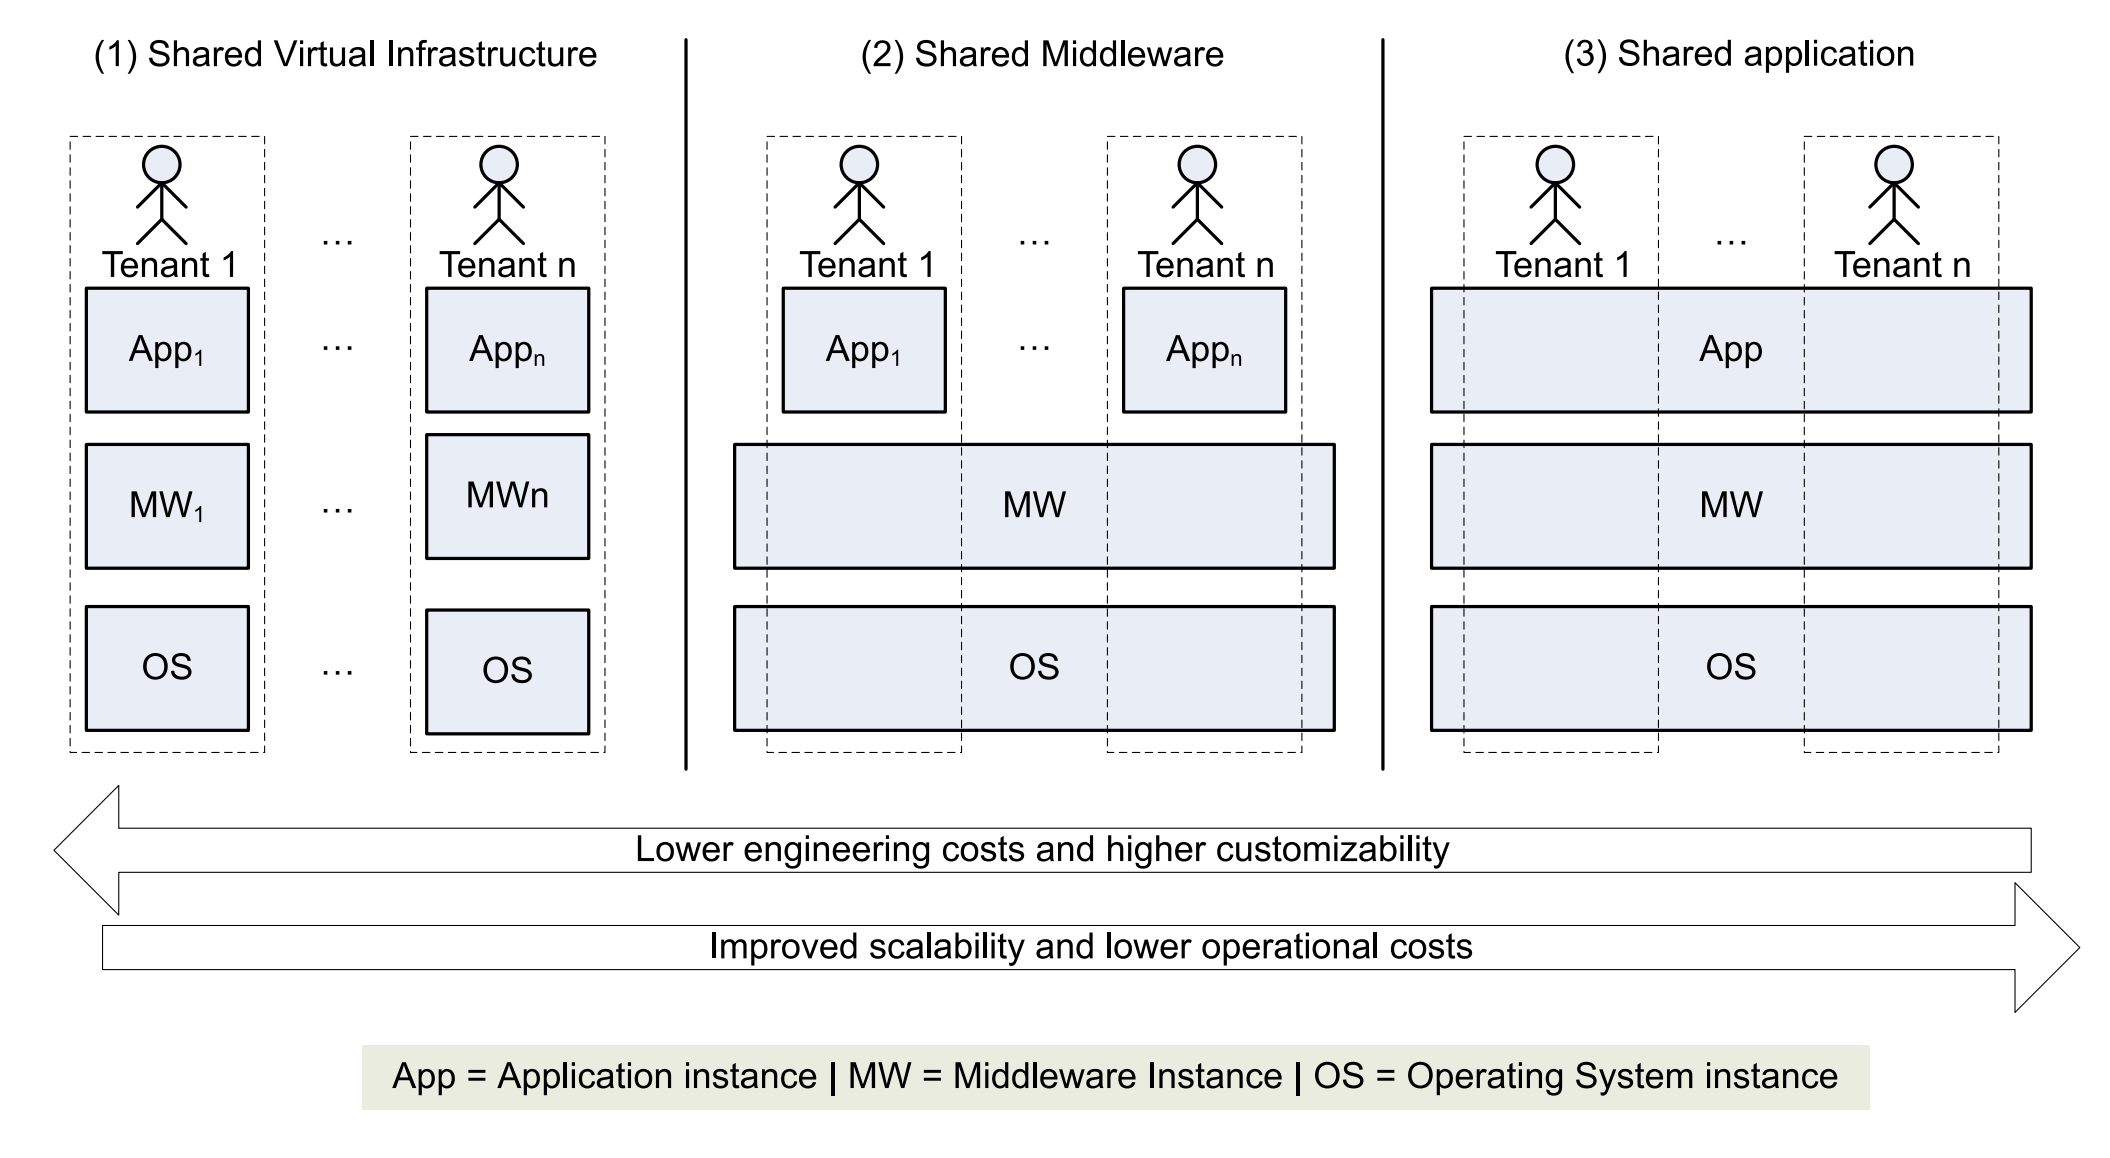
\includegraphics[width=0.65\textwidth]{chapter-background/muti-tenant-strategies.png}
\end{figure}


\section{Containerization}
Cloud providers rely on virtualization technology for the achievement of large-scale resource scaling. For more than a decade, virtual machines (VMs) have been the backbone of a provider's infrastructure offering hardware independence, availability, isolation and security~\cite{xavier2013performance}. More recently, containers a more lightweight virtualization technology have made advances in their multi-tenant capabilities and have seen an increase in adoption by providers~\cite{pahl2015containerization}. Both are discussed in this section.
\subsection{Virtualization technology}
In cloud environments, virtualization technology is used for flexible and dynamic allocation of physical resources to virtualized applications and to achieve multi-tenancy by sharing a physical server among multiple applications. In data centers virtualization is commonly used at the \textit{hardware level} and \textit{operating system level} to deploy and manage virtual machines and applications at scale~\cite{SharmaPrateek2016CaVM}. \\\\
Hardware level virtualization uses a hypervisor on a server to create virtual machines. Each virtual machine provides an abstraction of a physical machine and runs an independent operating system with applications. The hypervisor is responsible for resource allocation and performance isolation.\\\\
Operating system level virtualization allows resources to be shared at the level of the OS. Virtual machines running at the OS level are referred to as containers. Isolation, abstraction and resource allocation of containers is performed by the OS kernel of the host OS. By sharing the OS kernel among multiple containers, containers are regarded as a more lightweight virtualization technology. Containers only contain the application and its dependencies.\\\\
Linux containers (LXC)~\cite{lxc} employ different mechanisms of the Linux kernel to achieve resource isolation, namely control groups and namespaces.
\begin{itemize}
    \item \textbf{Cgroups}~\cite{cgroups} allow for fine-grained control of the allocation of system resources (CPU time, system memory, network bandwidth) among processes and process groups. For example, it is possible to limit or prioritize memory, CPU or I/O usage of different containers. 
    \item \textbf{Namespaces}~\cite{namespaces} allow for isolation of kernel resources among processes. A namespace makes a resource appear to be private and isolated for the container. The Linux kernel provides the following namespaces:  process ids, inter-process communication (IPC) mechanisms, network stack and mount points.
\end{itemize}
Linux containers (LXC) offers a lightweight implementation which performs at native speed and provides good isolation. However, while sharing a kernel between containers minimizes overhead, there are limitations in terms of the security environment.~\cite{dua2014virtualization}
\\\\
\noindent By offering virtualization at different levels, containers and VMs offer different trade-offs concerning performance isolation and performance. Research~\cite{SharmaPrateek2016CaVM} concludes that while containers offer closer to bare metal performance compared to VM, they offer worse performance isolation in multi-tenant environments. In addition, containers offer soft resource limits compared to the hard resource limits of virtual machines which allow for better server consolidation in over-commitment scenarios.  
\begin{figure}[h]
\caption{Container vs virtual machine.~\cite{container-vs-vms}}
\centering
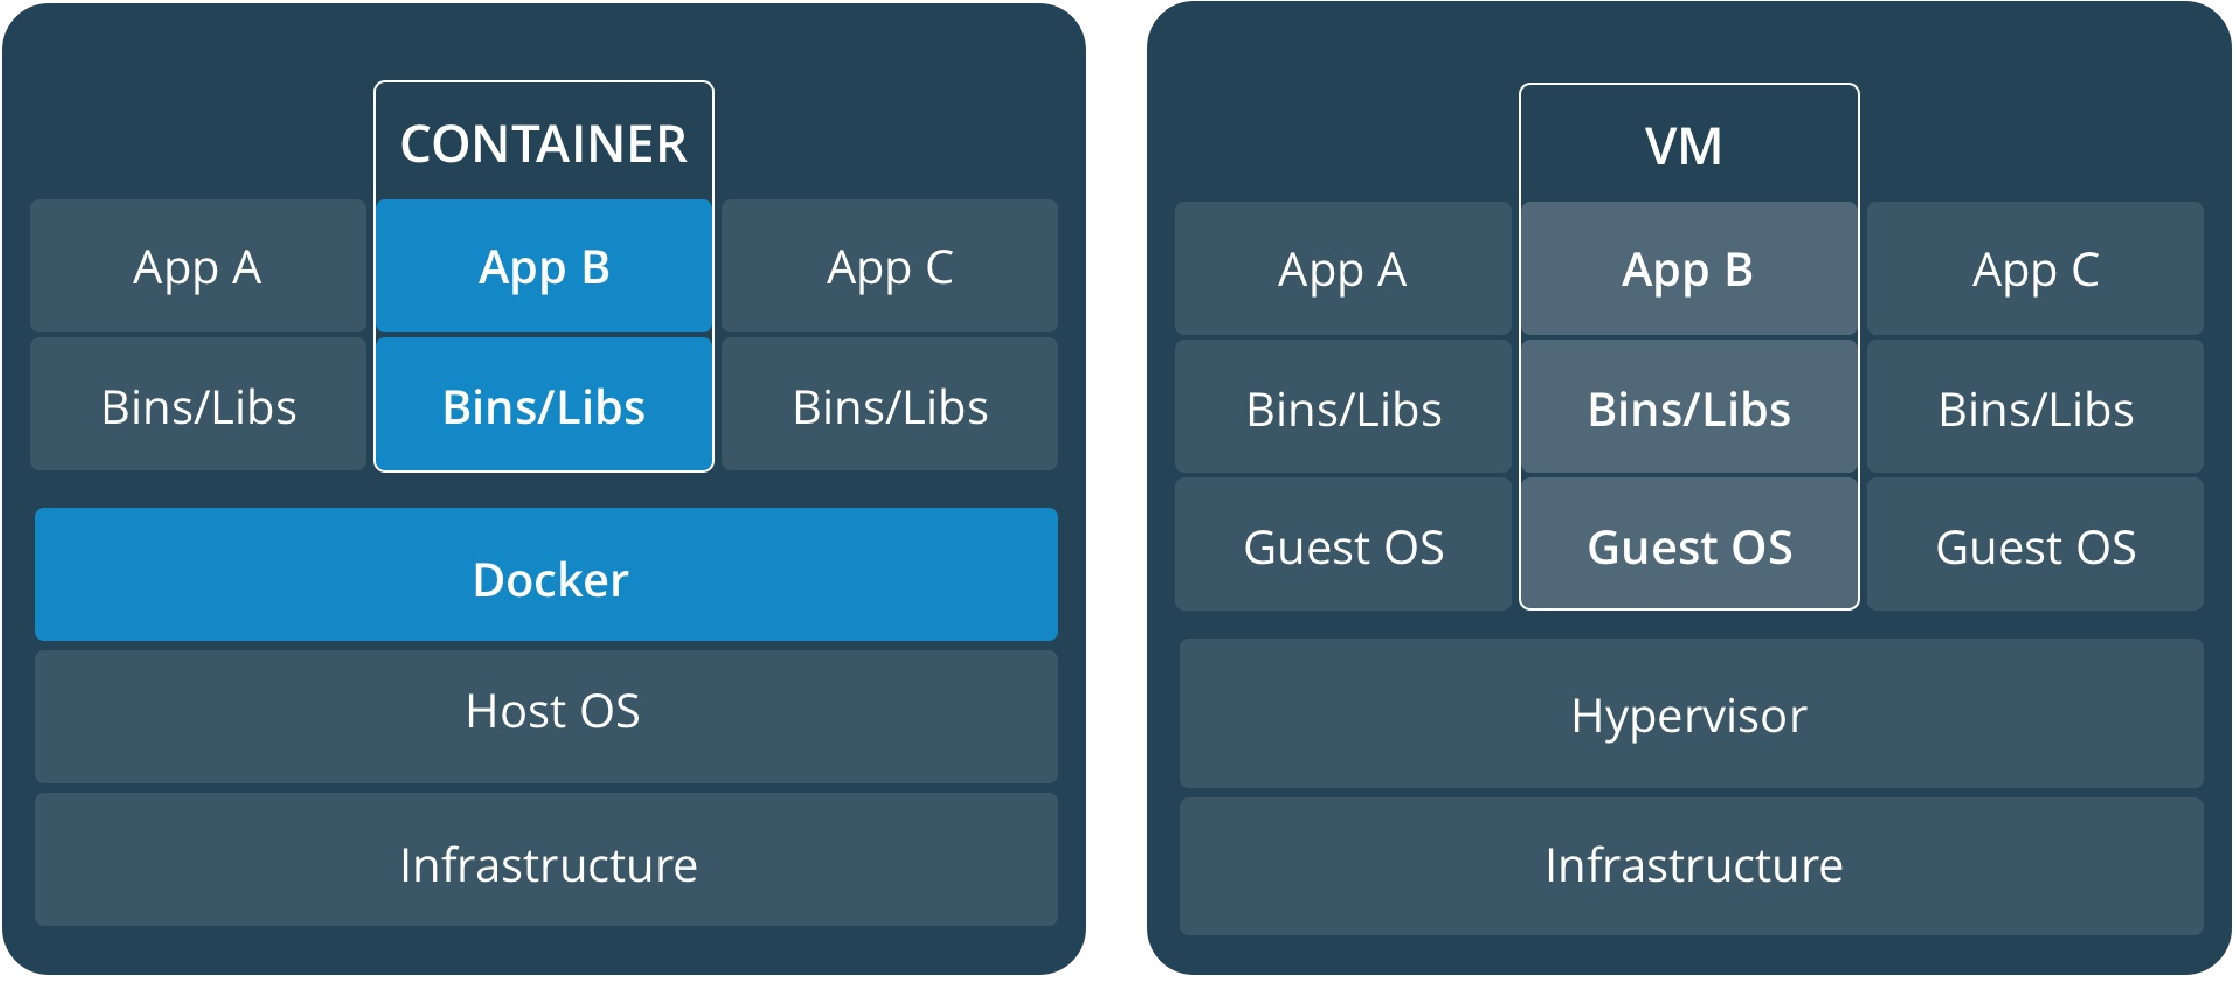
\includegraphics[width=0.8\textwidth]{chapter-background/containervsvm.pdf}
\end{figure}
\subsubsection{Docker}
Recently, thanks to Docker~\cite{dockersite}, containers have gained popularity and have been adopted into the software development process. However, Docker is not a new container technology, at its core it employs the kernel-level mechanisms of Linux containers (LXC), for which it defines a unified API~\cite{merkel2014docker}. In addition, the open-source Docker project offers a commandline-interface and daemon that offers easy packaging of applications in containers and the deployment of these containers.\\\\
To achieve this Docker introduces the concept of images. A container is represented by a lightweight image. A container image is a lightweight, executable package containing an application and its dependencies (runtime, libraries, environment variables, and config files). Virtual machines (VMs) can be seen as full, monolithic images. In particular,  Docker image consists of file-system layers stacked upon each other, as illustrated in Figure~\ref{docker-layers}. Only the top layer, the container itself, is writable, therefore it is state-full and executable. A container is thus composed out of layers of individual images built on top of a base image, allowing for easy extensibility.~\cite{pahl2015containerization} \\\\
A Docker image is specified by and build from a DockerFile. Images can be made easily accessible through Docker registries such as Dockerhub.\\
These images allow for easy and fast deployment of Docker containers across different operating systems and cloud provider stacks. Resulting in a game-changing technology for DevOps, system administrators and developers.
\begin{figure}[H]
\caption{Architecture of a container image. Images can be stacked upon each other using the cgroups and namespace extensions of a Linux kernel. The top container image is writable.~\cite{pahl2015containerization} \label{docker-layers}}
\centering
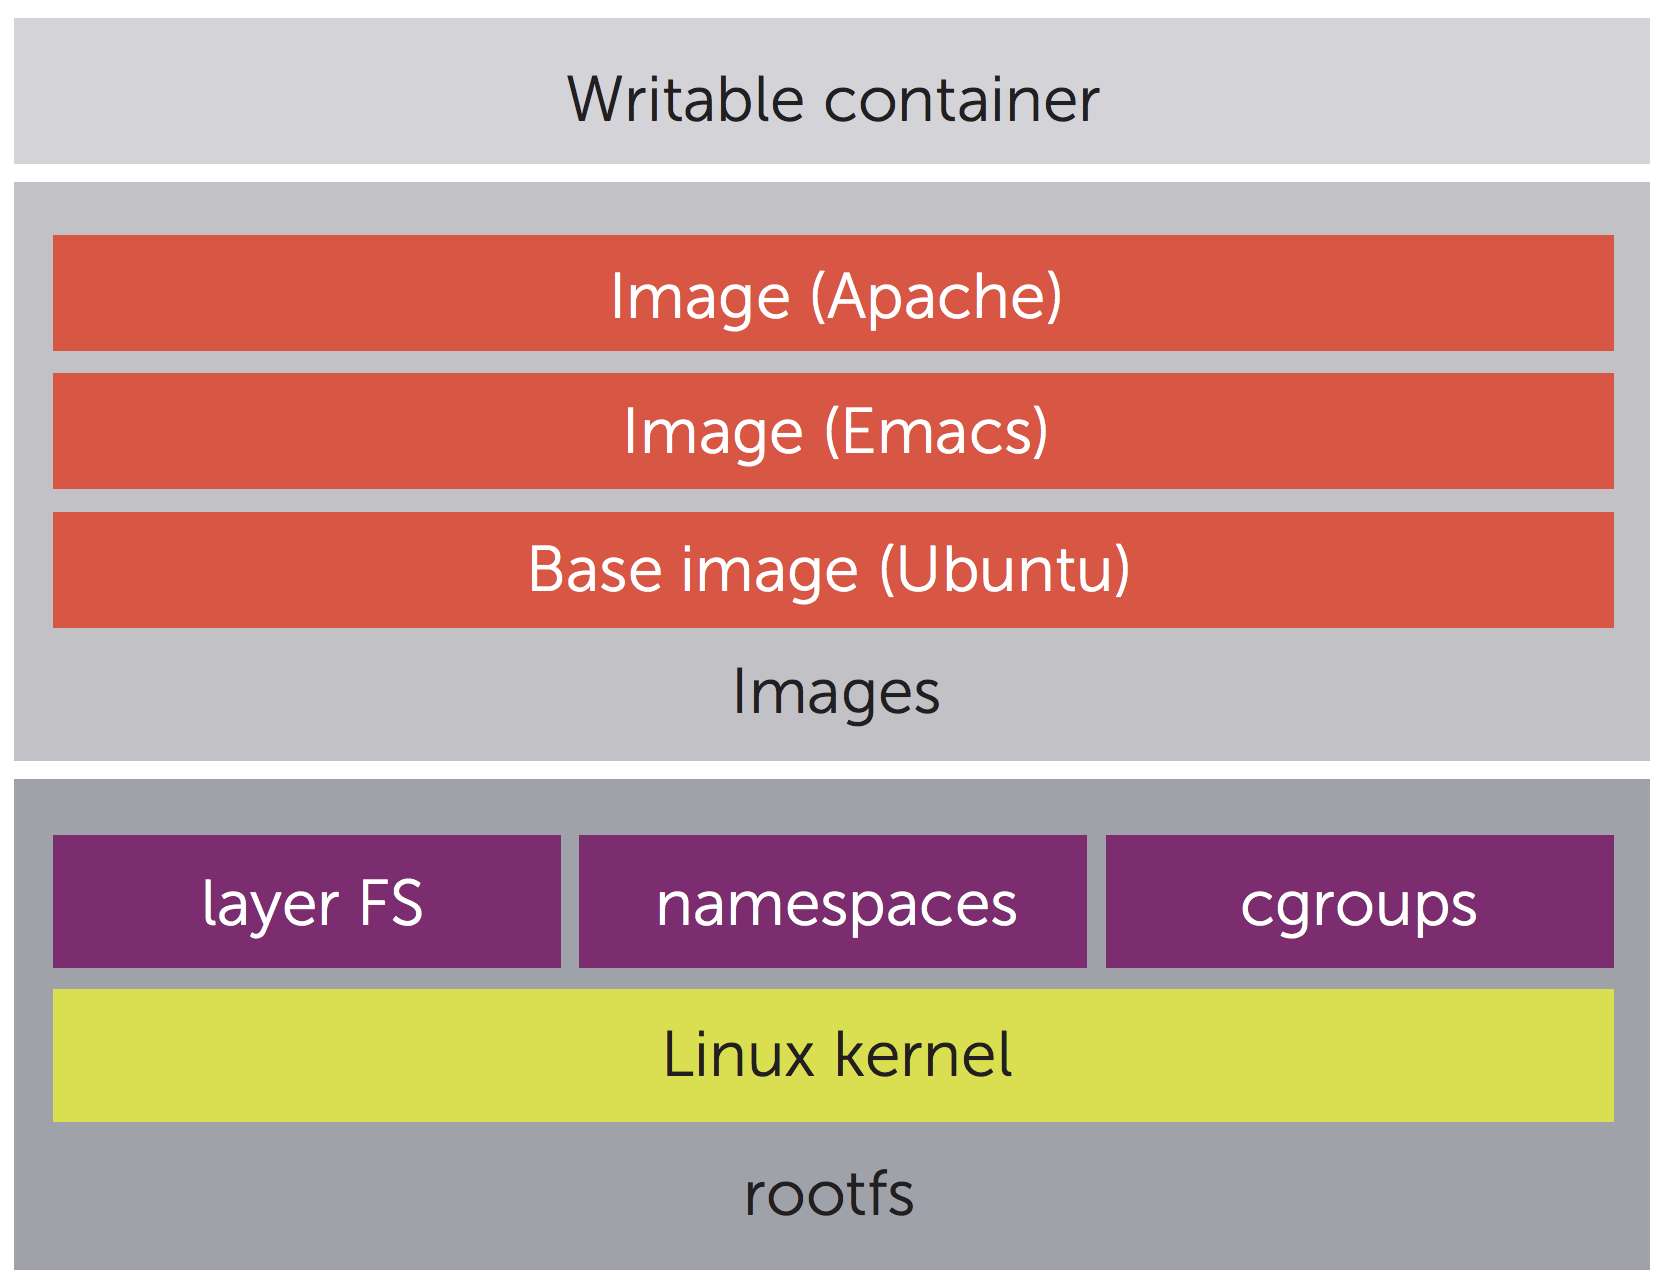
\includegraphics[width=0.5\textwidth]{chapter-background/docker-layers.png}
\end{figure}

\section{Container Orchestration}
Container technologies such as Docker offer advanced features to use containers in production. These solutions often offer deployment of applications limited to single machines. However, applications offered by  SaaS providers may include multiple different containers working together running on a cluster of nodes. Container orchestration (CO) systems allow deployment and management of containers at scale. Popular orchestration engines are Kubernetes, Docker Swarm and Mesos Marathon.
\subsection{Key capabilities of a container orchestration platform}
The task of a container orchestration (CO) platform is not limited to the initial deployment but the entire life-cycle of multiple containers. The goal of CO is to simplify cluster management while ensuring fault tolerance, availability, scalability and reliability. Allowing users to benefit from the complete potential of containers. In order to meet this goal, CO platform must at least offer the following key capabilities.~\cite{khan2017key}
\paragraph{Cluster state management and scheduling}
A cluster can be composed out of multiple virtualized or physical instances. Running containers on top of these instances and recover from failures requires a stable cluster. State management encapsulates various tasks such as flexible scheduling, re-partitioning of resources and data and propagating of dependent system changes.~\cite{khan2017key} 
\paragraph{High availability and fault tolerance}
A container orchestration platform must ensure high availability and fault tolerance in order to be useful for application developers. Most platforms therefor employ design principles of reliability engineering e.g., single point of failure elimination, failure detection or load balancing.~\cite{khan2017key}
\paragraph{Security}
Containers executing on top of the platform essentially form untrusted entities, with potentially malicious intentions, a high security standard is required. The standard should include: container images sanity check policies, access control for both containers and users, and techniques to minimize the container attack surface.~\cite{khan2017key}  
\paragraph{Simplified networking}
Containers must be able to communicate across nodes in  an efficient and secure manner. This requires the mapping of allocated host ports to containers. The overhead corresponding to this mapping intensifies at scale. The CO platform should thus provide a flexible, secure and scalable solution for networking.~\cite{khan2017key}
\paragraph{Service discovery}
The large number of services present in a cluster need to be able to communicate with each other. In traditional clusters services were handled as pets (i.e, having static names, IP addresses), however, in dynamic environments such as container orchestration platforms, they are regarded as cattle. The CO platform must provide mechanisms for addressing/labeling/grouping and service discovery.~\cite{khan2017key} 
\paragraph{Monitoring and governance}
The container orchestration platform needs to support traditional monitoring techniques such as logging, resource usage and network trace-routes. Monitoring must be possible at both the level of the underlying infrastructure and the containers themselves.~\cite{khan2017key}
\paragraph{Integrating for continuous integration and delivery}
Software development teams should be able to integrate the CO platform within their employed continuous integration and delivery (CI/CD) pipeline. The CO platform should contain mechanisms for rolling updates, rollbacks, etc.~\cite{khan2017key}


\subsection{Kubernetes}
Kubernetes~\cite{kubernetes}, commonly referred to as K8,  is one of the most popular and adopted orchestration systems. It is an open-source project led by Google. Kubernetes is Google's solution for the growing demand of container deployments by external developers in its public business cloud and is based upon its predecessors  Borg~\cite{verma2015large} and Omega~\cite{schwarzkopf2013omega} that have been used to schedule the internal Google workload. Its main design goal is formulated as:\textit{ "to make it easy to deploy and manage complex distributed systems, while still benefiting from the improved utilization that containers enable~\cite{Burns:2016:BOK:2930840.2890784}"}.  \\\\
\noindent To achieve the above stated goal Kubernetes introduces a number of concepts for both containers and cluster resources. It implements the infrastructure as code model  by provides an abstraction layer on top of the physical infrastructure~\cite{hermanns2015current}. It allows to setup and manage container infrastructure by the configuration of these introduced concepts via a REST API or declarative YAML configuration files. Below the most relevant concepts are introduced.
\subsubsection{Kubernetes concepts}
\textbf{Pods.}  A pod is the smallest unit of deployment within Kubernetes. It is a group of one or more containers that logically belong together.   A pod and thus its containers run on the same node. They share the same network, storage and context (Linux namespaces, cgroups). A pod gets assigned a unique IP address. Pods are not self-healing meaning when an error occurs within the pod or during scheduling. It will be deleted. Due to this short life cycle using a single pod resource and its assigned IP address for applications is impractical. Kubernetes handles this by employing controllers and services.~\cite{pods}\\\\
\textbf{Deployments.}  A Deployment controller manages a pod or a ReplicaSet of pods. A ReplicaSet allows pods to be replicated across multiple nodes. A Deployment object is used to specify the desired state of pods (e.g. number of replica's). A deployment, in addition, allows for declarative updates. These updates can be used to change the number of container replicas of a ReplicaSet or to update a specific container image within the pod.  The Deployment controller changes the actual state to the desired state described by the update.~\cite{deployments}
\\\\
\textbf{Services.}  Services offer a solution for the short life cycle of pods (and their IP addresses). Services within Kubernetes offer a manner to expose a ReplicaSet of Pods via a unique name, stable IP address, network policy and ports. To determine which set of pods is targeted by a service, Kubernetes employs a Label selector. Labels are the core grouping primitive of Kubernetes and unlike names and UIDs do not offer uniqueness.\\  A Service can be exposed outside the cluster by using an external load balancer or by specifying a NodePort. When using a Nodeport each node within the cluster will expose the port and forward request into the service.~\cite{services}
\\\\
\textbf{Namespaces.}  Namespaces allow to partition resources of a physical cluster among multiple user organizations. Each namespace gets a share of the resources of the cluster, via resource quotas. Resource quotas are supported for CPU, memory and persistent volumes.~\cite{namespaces-k8}
\\\\
\textbf{Resource limits.}  Kubernetes allows the allocation of compute resources of both containers and Namespaces by the means of resource limits. These limits can be soft (limit) and hard (request) limits. A Request specifies the quantity of resource that is guaranteed to the container. A limit specifies the maximum quantity allocated to the container. When the requested resource quantities of a container are less than its limit, the container may be allocated additional resources if there are unallocated resources available.  The current supported compute resources are CPU, memory and storage within the root partition of the local node. Within a Pod it is possible to specify both request and limit for each container. When request and limits are specified, the scheduler will use them for both scheduling and eviction (when node capacity is reached) decisions.~\cite{kubresources}
\subsubsection{Kubernetes architecture}
The basic architecture of Kubernetes is illustrated in Figure~\ref{fig:kubarch}. A client-server architecture is employed in which master and node setups are deployed on different machines. Below the different components that build up the architecture are briefly explained. 
\paragraph{API Server.} The API server is responsible for the configuration and validation of API objects (pods, deployments, services,...). It offers communication on cluster state via a REST interface for both components and administrators.~\cite{kubernetes-api-server}
\paragraph{Controller manager.} The controller manager is responsible for managing several core control loops part of Kubernetes. A control loop uses the API server to observe the shared state of the cluster and attempts to move to the desired state via configuration changes.~\cite{kubernetes-controller-manager}
\paragraph{Scheduler.} The task of assigning pods to nodes is the responsibility of the scheduler component.  The scheduler attempts to do a reasonable placement based on resource and quality of service requirements (e.g., not place a pod on a node with insufficient resources). It is  possible for users to control the placement of pods via NodeSelector tags or affinity and anti-affinity constraints in the configuration file.~\cite{kubernetes-pods-to-nodes,kubernetes-scheduler}
\\\\In addition it is possible to assign Quality of Service (QoS) classes to pods. These are used by Kubernetes in the decision process about scheduling and eviction of pods. Currently, Kubernetes supports three types of classes: guaranteed, burstable and best-effort. In decreasing order of priority (i.e., most likely to be killed in the case of resource shortages). The QoS classes are assigned to pods based on the presence of request and limit specifications of resources in their configuration files.~\cite{kubernetes-qos}


\paragraph{Kubelet.} The kubelet component is an agent running on each node. It is responsible for running and maintaining pods on its residing node. The set of maintained pods is described in the form of PodSpecs (mainly received via the API-server).~\cite{kubernetes-kubelet}
\paragraph{Kube-proxy.} The kube-proxy daemon provides a simple network proxy for the services on each node. It enables forwarding of requests to the correct containers and can provide primitive load balancing.~\cite{kubernetes-kubeproxy}
\begin{figure}[H]
\caption{Kubernetes architecture}
\centering
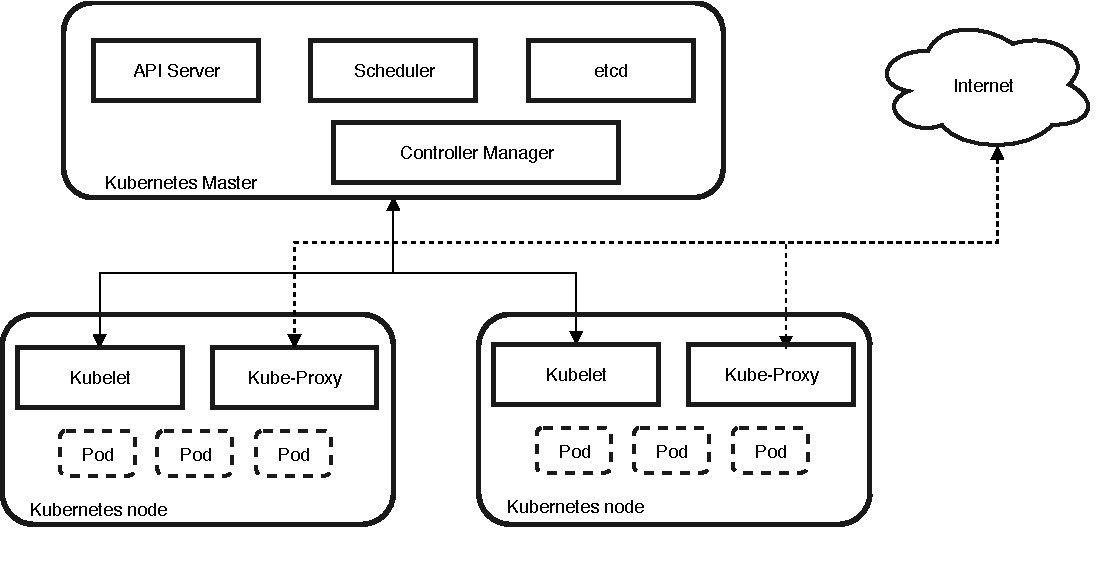
\includegraphics[width=0.8\textwidth]{chapter-background/kubernetes-architecture-diagram.pdf}
\label{fig:kubarch}
\end{figure}
 
 
 
 
 
 
 
 
 
 \section{Performance evaluation}
As discussed in previous sections, SaaS providers employ multi-tenancy to improve  cost efficiency and offer several performance guarantees to their customers in the form of SLOs. An unavoidable consequence of multi-tenancy is the need to support a growing number of users in a single system. Providers need to have a clear insight into the \textit{scalability} of their systems. However, scalability is a difficult thing to define, let alone quantify. Citing the words of  Dr. Neil J. Gunther:  \textit{"if you can't quantify it, you can't guarantee it"}.~\cite{perfdynamics}

\subsection{The Universal Scalability Law}
\label{section-USL}
Dr. Neil J. Gunther provides a formal definition of scalability: \textit{"scalability can be defined as a mathematical function, a relationship between independent and dependent variables (input and output)"~\cite{perfdynamics}}. The Universal Scalability Law (USL) by Dr. Neil J. Gunther is presented in Equation~\ref{USL}. It computes the relative capacity $C(N)$ at a load of $N$ users. Relative capacity is the normalized throughput.
\begin{equation}
\label{USL}
C(N) = \frac{\gamma~N}{1 + \alpha~(N-1) + \beta~N~(N-1)}
\end{equation}

The Universal Scalability Law incorporates factors that contribute to the sublinearly scalability of most systems. Namely, \textbf{concurrency} ($\gamma$), \textbf{contention} ($\alpha$) and \textbf{coherency} ($\beta$) as explained below. Their impact is visualized in Figure~\ref{fig:usl-impact}.

\begin{itemize}
    \item \textbf{Concurrency}($\gamma$): $\gamma$ defines the slope if the system was linearly scaling i.e., $C(N) = \gamma N$. It has been referred to as the \textit{coefficient of performance} by~\cite{schwarz2015practical}.
    \item \textbf{Contention} ($ \alpha $) : When scaling most systems parallelism while be limited at some point by contention (i.e., waiting or queuing for shared resources). The maximum speedup by parallelism is limited by the serialized portion ($\alpha$) of the work~\cite{schwarz2015practical}. 
    \item \textbf{Coherency} ($\beta$): created by crosstalk between components. Because crosstalk is possible between each pair of components in the system, the penalty grows quadratic $N(N-1)$.~\cite{schwarz2015practical}
    
\end{itemize}

\begin{figure}
    \centering
    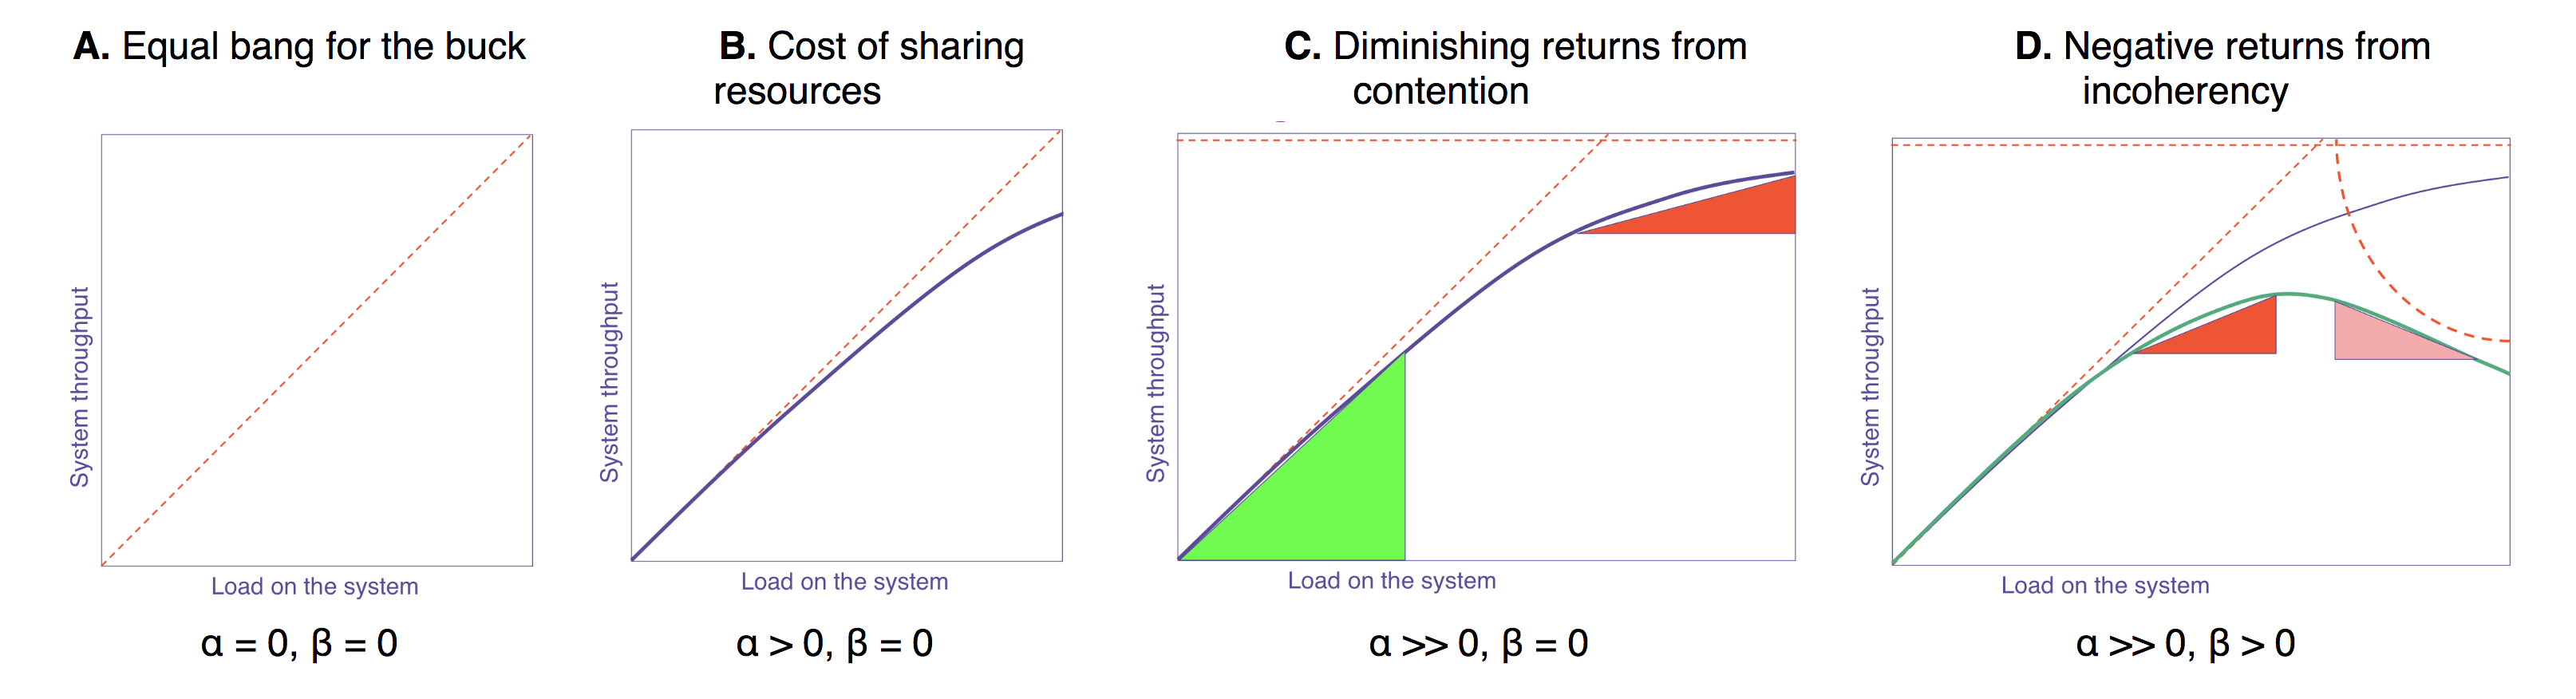
\includegraphics[width=1.1\textwidth]{chapter-evaluation/usl-impact}
    \caption{The impact of different USL coefficients on scalability.~\cite{perfdynamics}}
    \label{fig:usl-impact}
\end{figure}

\subsubsection{USL in practice}
USL can provide insights into a system's scalability pains via  values of the concurrency, contention and coherency coefficients. These can be obtained by collecting a dataset of measurements of the system, system load $N$ and corresponding throughput, and using a statistical technique such as nonlinear least square regression which fits the USL to the dataset.~\cite{schwarz2015practical,heyman2014scalability}

\subsection{Little's law}
\label{sec:little}
The Universal Law of Scalability serves as an alternative for the often less intuitive queuing models frequently used for modeling scalability. It omits the need to know the service time for every queue in the performance model in order to predict the response time or latency~\cite{perfdynamics}. Nevertheless, queuing theorem and its lemmas such as Little's Law can provide useful insights into performance modeling.\\\\
John D.C Little's Law~\cite{little2008little} states the following for stable systems: 
\begin{displayquote}
\textit{"The average number of items in a queuing system equals the average rate at which items arrive multiplied by the average time that an item spends in the system.\cite{little2008little}"}
\end{displayquote}
\begin{equation}
\label{littleslaw}
L = \lambda~W
\end{equation}
\begin{equation}
\label{llsys}
N = X~Rt
\end{equation}
Equation~\ref{littleslaw} shows Little's law, below its terms and its applicability to web services (Equation~\ref{llsys}) are explained:
\begin{itemize}
    \item \textbf{$L$}:  Average number of items in the system. For a web service this is represented by the average number of concurrent users in the system $N$.
    \item \textbf{$\lambda$}: Long-term average arrival rate of items in the system per time unit. Little's law assumes a stable system for which the arrival rate and exit rate are identical. In a web service this is represented by the throughput $X$.
    \item \textbf{$W$}: Average waiting time of an item in the system, queuing time and service time combined. This is represented by the response time $Rt$ or latency of a request in a web service. When dealing with a system involving think time (e.g., after the response from a web service, a user needs time to think about his/her next request), $(Rt + Zt)$ is used. 
\end{itemize}

\subsubsection{Workload generator validation}
Developers employ software tools (JMeter~\cite{jmeter}, Locust~\cite{locust}, etc.)  to simulate a workload and test the performance of a system. A workload is a set of actions that represent the behavior of a client in the system. It is part of the test plan stating the number of concurrent users $N$ executing the workload for a specified period of time.\\\\
The results of a performance test are typically expressed in throughput $X$ and response time $Rt$. Using Little's law it is possible to validate these results. For example, a test plan of 1000 concurrent users $N$ results in a throughput of 50 requests per second and an average response time of 15 seconds. Following Little's law, a concurrence of only 750 users was reached, instead of the specified 1000. Little's law can thus be used to check if a workload generator works as specified.\\\\
Alternatively, if the average throughput and response time for a production system are known, Little's law can be used to correctly draw up a test plan.

\subsubsection{Response time or latency?}
Performance can either be measured in throughput or latency, both are correct but offer a different point of view. System performance is typically expressed in throughput: "The system can handle a million operations per second". However, users care more about their personal experience with a system which is influenced by the average latency of their request.~\cite{schwarz2015practical} \\\\
Figure~\ref{fig:ls_vs_tp} shows the relation between the average latency and throughput of a database under increasing load $N$. In this case, latency is kept stable by increasing the throughput with the increasing load up to a certain point.  A bottleneck caps the throughput of the systems and by Little's law for an increasing load and constant throughput, the latency must increase.~\cite{latvsthrough} \\\\
However in other systems, as discussed in Section~\ref{section-USL}, an increasing load might induce a diminishing result on the system's throughput. Following Little's law a decreasing throughput results in a higher latency under the same load. \\\\
Thus, for stable systems by Little's law,  the USL can be reformulated in terms of latency instead of throughput. Equation~\ref{USL-2} shows this reformulation.~\cite{schwarz2015practical}
\begin{equation}
\label{USL-2}
Latency(N) = \frac{1 + \alpha~(N-1) + \beta~N~(N-1)}{\gamma}
\end{equation}


\begin{figure}[H]
    \centering
    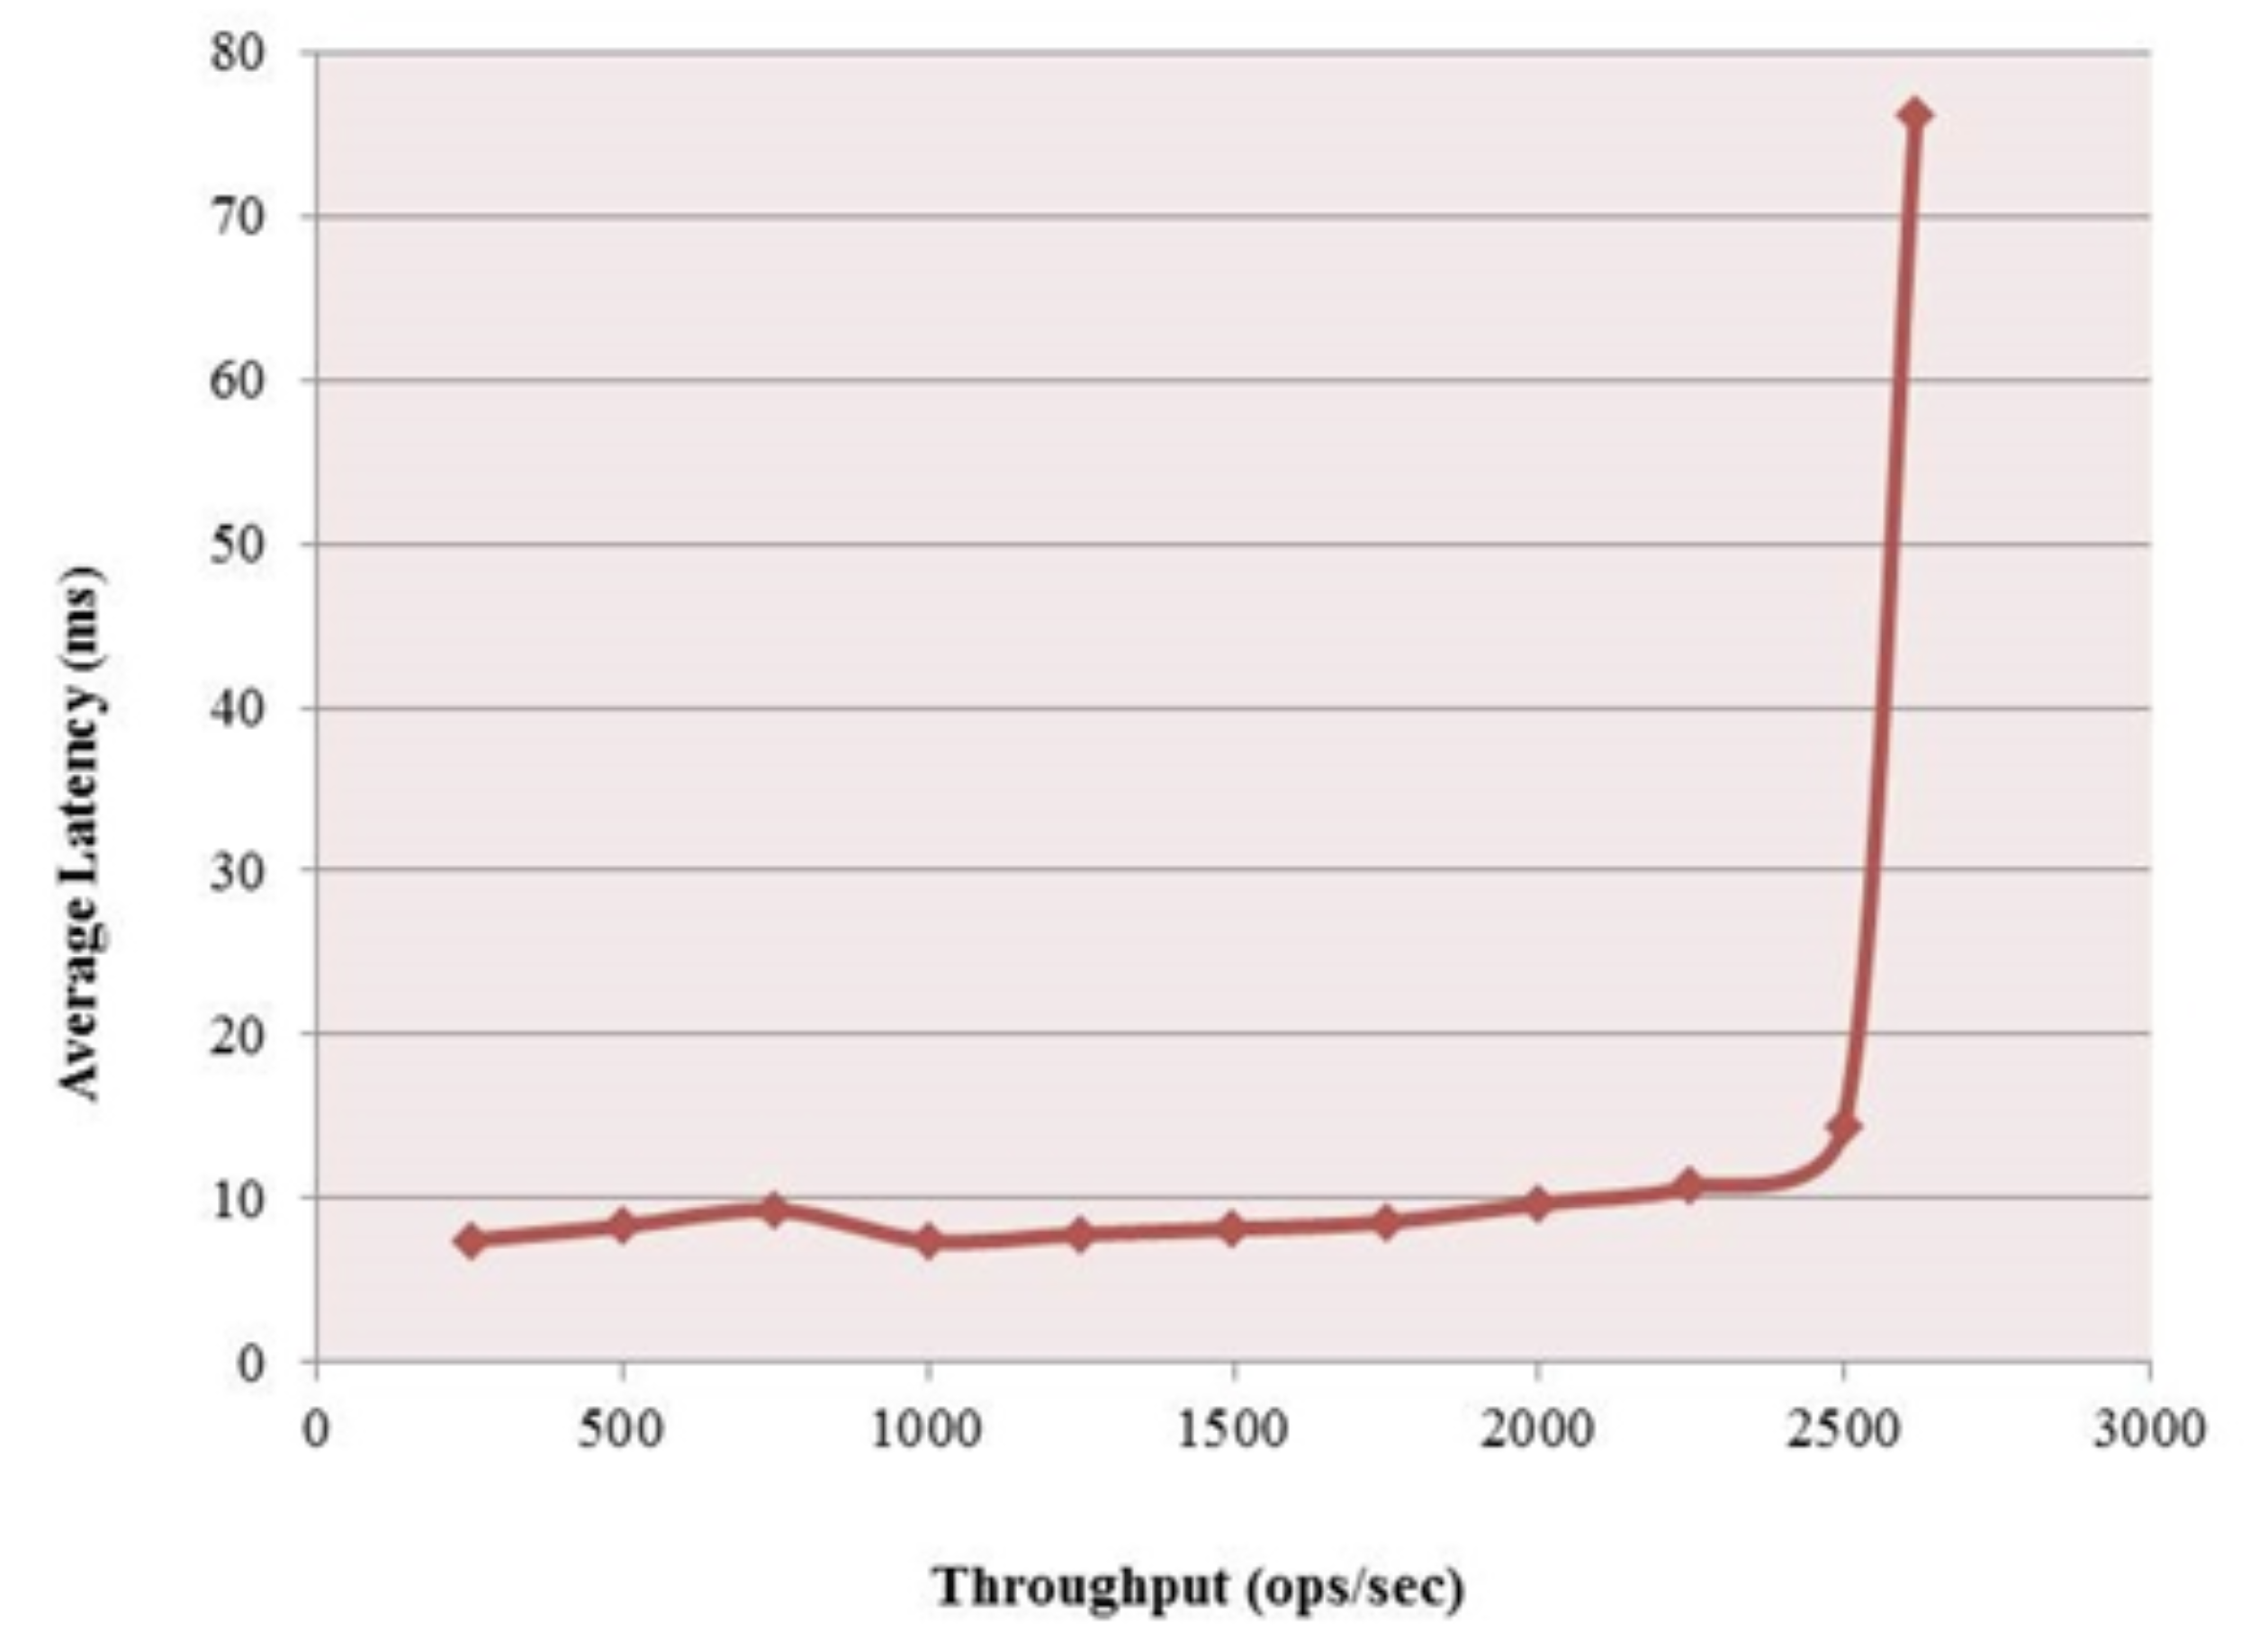
\includegraphics[width=0.8\textwidth]{chapter-evaluation/ls_vs_th}
    \caption{Relation average latency vs. throughput for database benchmark with increasing load.~\cite{latvsthrough}}
    \label{fig:ls_vs_tp}
\end{figure}
\chapter{Background}
\label{ch:background}
This chapter discusses relevant background material for the thesis. The concepts, explored in this chapter, further clarify the relevance of the thesis and serve as building blocks for the remaining chapters. Starting from the adoption of the cloud computing paradigm, the chapter elaborates on how concepts such as multi-tenancy and virtualization via containerization push the limits of efficient resource utilization. Next, an in-depth overview of the open-source container orchestration platform Kubernetes is provided. Lastly, insights are provided into the universal scalability law and the applicability of Little's law for performance testing.
\section{Cloud computing}
Companies try to minimize the total cost of ownership by moving to cloud computing or utility computing. The cloud computing paradigm enables on-demand access to a shared pool of configurable compute resources (software applications, system software and hardware infrastructure)~\cite{WalravenStefan2015PPmf}. A service provider can provision the required resources from the cloud with minimal effort.  Within this paradigm, services are offered in real time over the internet in three different models~\cite{MellPeter2010TNDo,rimal2009taxonomy}. 
\begin{itemize}
\item \textit{Infrastructure as a Service (IaaS)} in which access is offered to virtual machines, network, data storage and other fundamental computing resources. The customer is able to deploy arbitrary software using these resources.\\\\
Examples: Digital Ocean, Microsoft Azure and Amazon Elastic Compute Cloud (EC2).
\item \textit{Platform as a service (PaaS)} offers customers a platform enabling easy and efficient deployment of applications (at scale) while abstracting the complexity of managing the underlying infrastructure. PaaS allows customers to solely focus on the development of their application.\\\\
Examples: Google app engine, Microsoft Azure and Heroku.
\item \textit{Software as a service (SaaS) } allows customers to make use of a specific application developed by a SaaS provider. Compared to the traditional use of software, the management and deployment is the task of the SaaS provider. In this strategy, common resources and a single instance of both the application and underlying database are used to support multiple customers simultaneously. \\\\
Examples: Google apps and Salesforce.
\end{itemize}

\section{Multi-tenancy}
\label{multi-tenancy}
The software as a service (SaaS) model offers applications to customers as an on-demand service. Providers of these applications try to leverage economies of scale by employing a multi-tenancy architectural design principle. The goal of multi-tenancy is to minimize the total cost of ownership for the provider by maximizing the sharing of resources among multiple customers organizations, referred to as tenants.~\cite{Walraven2015b} 
\subsection{Service Level Agreements}
By moving their core business functions to an entrusted cloud provider, cloud customers give up control of the underlying compute resources. It is vital for these tenants to obtain certain guarantees on the service delivered by the provider. 
A Service Level Agreement (SLA) is a formal contract between the SaaS provider and the tenant specifying both properties of the provided service and the expected behavior of the tenant. An SLA typically also contains a set of Service Level Objectives (SLOs). An SLO is a measurable characteristic of the service. An SLO is typically related to performance constraints (latency, throughput and deadlines) or availability (uptime percentage) of the service. Within the specification of an SLA a trade-off must often be made between expressiveness and usability. The SLA must cover all the expectations of a customer while remaining simple to weight, verify, evaluated and enforce~\cite{dillon2010cloud}.  Some typical examples of SLOs are shown below: 
\begin{itemize}
\item The application has a monthly uptime percentage of 99.95\%.
\item If the arrival rate of the tenant workload < X requests/s then a throughput T is guaranteed.
\end{itemize}
\subsection{Challenges}
While the goal of multi-tenancy is promising, sharing a cluster of dynamically provisioned nodes between multiple tenants imposes a number of challenges and requirements~\cite{TruyenEddy2016Taca}. 
\begin{itemize}
\item Performance isolation: the activities of one tenant should not be able to influence the service level delivered to other tenants. This requirement should be achieved during normal system load and when an aggressive tenant violates the terms of the SLA. 
\item QoS differentiation: the performance guarantees specified by an SLA can be individually customized for each tenant. A SaaS provider should be able to offer different subscriptions.
\item Flexible resource allocation for improved server consolidation: a SaaS provider employs a multi-tenant architecture to achieve a lower operational cost. This is partially achieved by planning the required node capacity based on the actual resource usage of tenants instead of the theoretical required capacity.  This can be further aided by the use of request schedulers allowing to distinguish between normal, passive and aggressive tenants. 
\end{itemize}
\subsection{Strategies}
To achieve multi-tenancy different strategies, each offering different trade-offs concerning operational costs and upfront application engineering costs, can be employed by the SaaS-provider~\cite{WalravenS.2011Amlf}. The strategies are illustrated in Figure~\ref{muti-tenant-strategies}.
\begin{itemize}
\item Multi-tenancy can be achieved at the level of the \textit{operating system}. In this strategy, a virtualization technology can be used to partition compute resources among multiple virtual machines. Each tenant is assigned an application instance running on a dedicated virtual machine. This approach offers both a higher level of performance isolation and lower upfront engineering costs but suffers from an inefficient utilization of resources.
\item In \textit{middleware-level multi-tenancy} a middleware platform is used to enable sharing compute resources between multiple tenants at the level of the operating system. An application instance is deployed on top of the middleware platform for each tenant. By not replicating the operating system for each tenant a higher level of cost efficiency can be achieved but an increased complexity in managing resources and  performance isolation is introduced. By tackling these problems at the level of the middleware a part of the engineering complexity is shifted to this level.
\item The most efficient resource utilization can be achieved by sharing application instances between multiple tenants. In \textit{Application-level} multi-tenancy achieving performance isolation is done by the application itself thereby increasing the engineering complexity and costs.
\end{itemize}


\begin{figure}[H]

\caption{Different strategies to achieve multi-tenancy~\cite{WalravenS.2011Amlf}.\label{muti-tenant-strategies} }
\centering
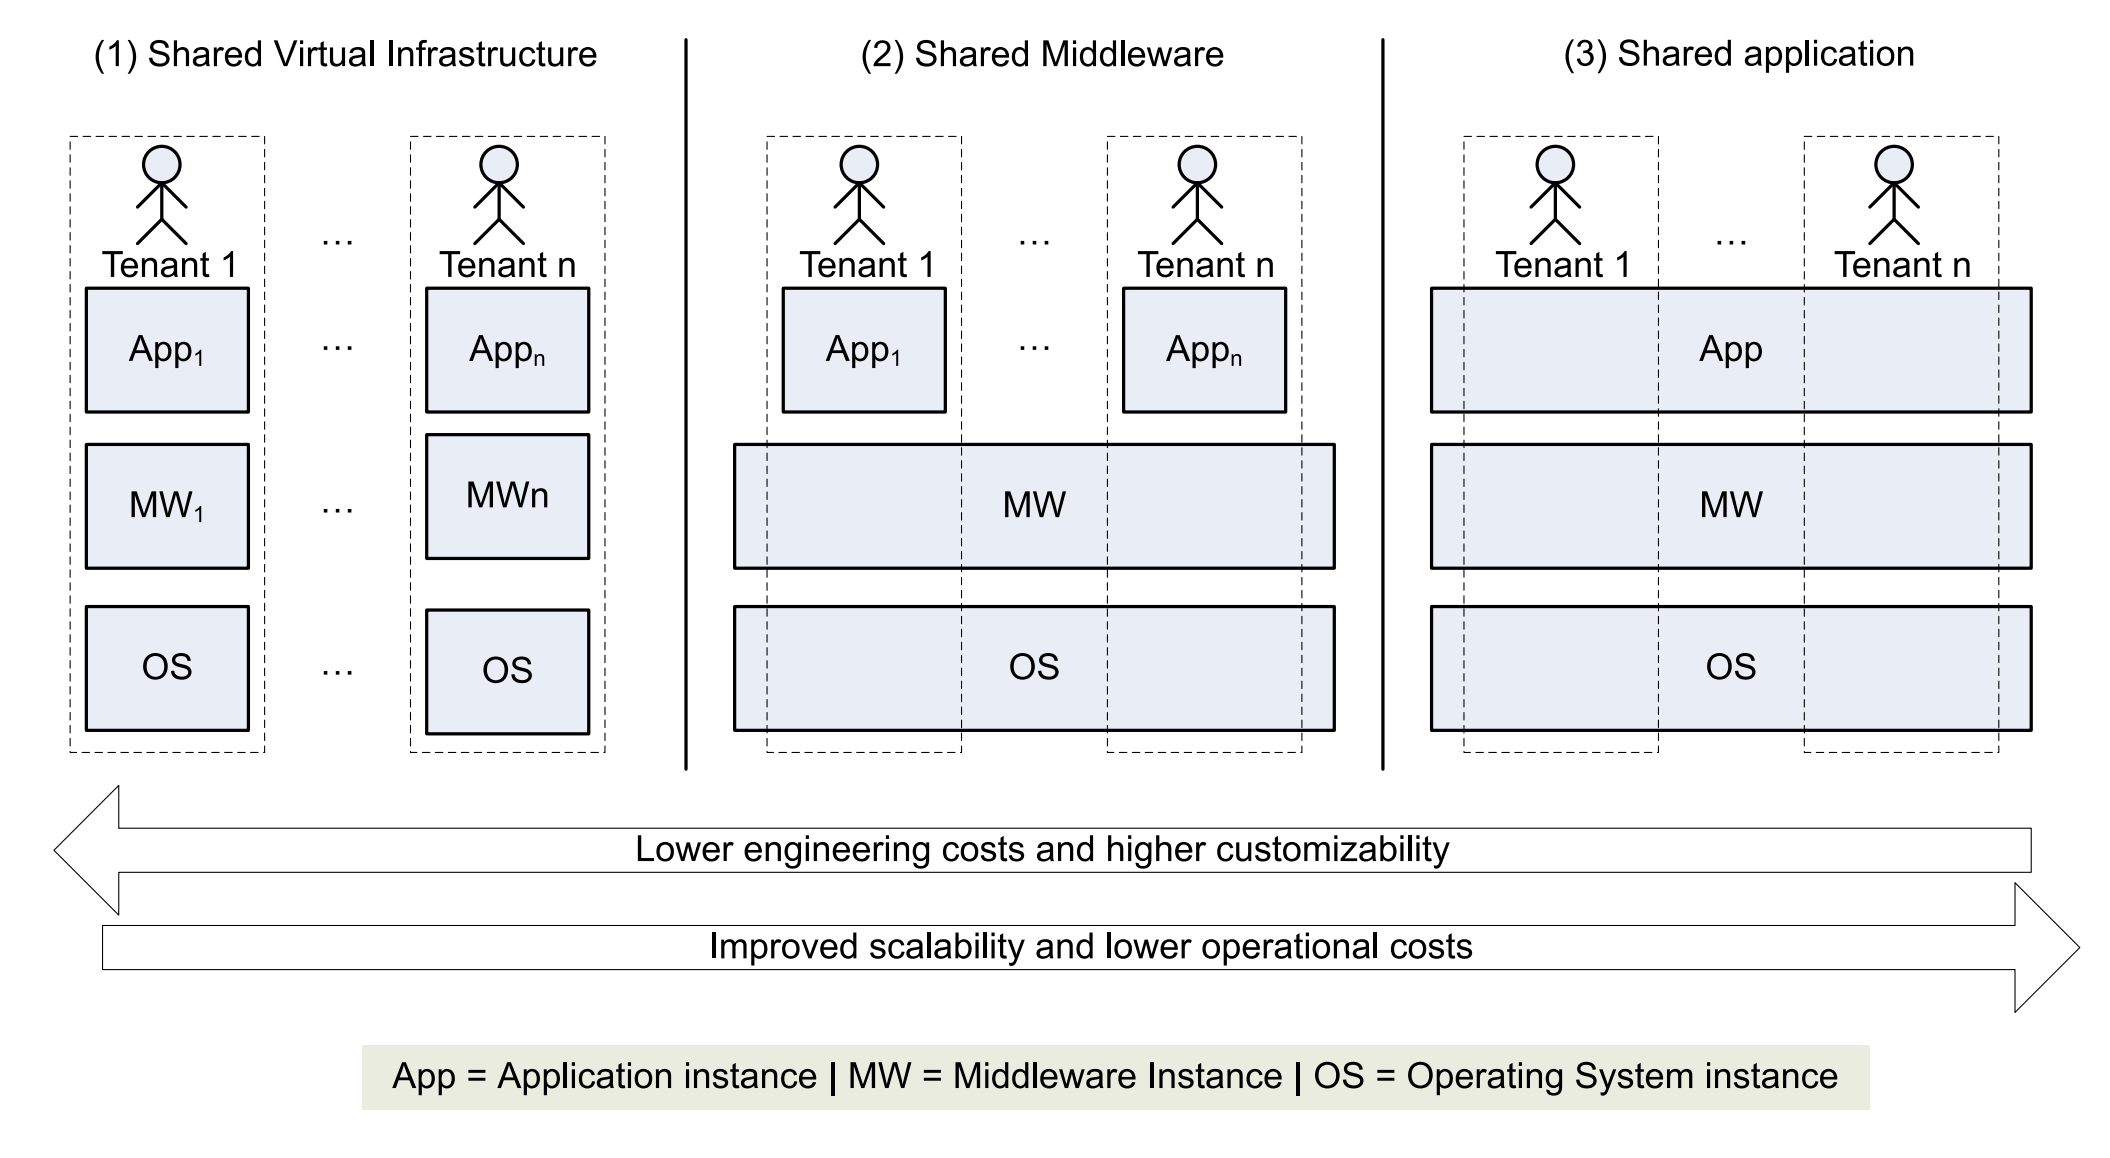
\includegraphics[width=0.65\textwidth]{chapter-background/muti-tenant-strategies.png}
\end{figure}


\section{Containerization}
Cloud providers rely on virtualization technology for the achievement of large-scale resource scaling. For more than a decade, virtual machines (VMs) have been the backbone of a provider's infrastructure offering hardware independence, availability, isolation and security~\cite{xavier2013performance}. More recently, containers a more lightweight virtualization technology have made advances in their multi-tenant capabilities and have seen an increase in adoption by providers~\cite{pahl2015containerization}. Both are discussed in this section.
\subsection{Virtualization technology}
In cloud environments, virtualization technology is used for flexible and dynamic allocation of physical resources to virtualized applications and to achieve multi-tenancy by sharing a physical server among multiple applications. In data centers virtualization is commonly used at the \textit{hardware level} and \textit{operating system level} to deploy and manage virtual machines and applications at scale~\cite{SharmaPrateek2016CaVM}. \\\\
Hardware level virtualization uses a hypervisor on a server to create virtual machines. Each virtual machine provides an abstraction of a physical machine and runs an independent operating system with applications. The hypervisor is responsible for resource allocation and performance isolation.\\\\
Operating system level virtualization allows resources to be shared at the level of the OS. Virtual machines running at the OS level are referred to as containers. Isolation, abstraction and resource allocation of containers is performed by the OS kernel of the host OS. By sharing the OS kernel among multiple containers, containers are regarded as a more lightweight virtualization technology. Containers only contain the application and its dependencies.\\\\
Linux containers (LXC)~\cite{lxc} employ different mechanisms of the Linux kernel to achieve resource isolation, namely control groups and namespaces.
\begin{itemize}
    \item \textbf{Cgroups}~\cite{cgroups} allow for fine-grained control of the allocation of system resources (CPU time, system memory, network bandwidth) among processes and process groups. For example, it is possible to limit or prioritize memory, CPU or I/O usage of different containers. 
    \item \textbf{Namespaces}~\cite{namespaces} allow for isolation of kernel resources among processes. A namespace makes a resource appear to be private and isolated for the container. The Linux kernel provides the following namespaces:  process ids, inter-process communication (IPC) mechanisms, network stack and mount points.
\end{itemize}
Linux containers (LXC) offers a lightweight implementation which performs at native speed and provides good isolation. However, while sharing a kernel between containers minimizes overhead, there are limitations in terms of the security environment.~\cite{dua2014virtualization}
\\\\
\noindent By offering virtualization at different levels, containers and VMs offer different trade-offs concerning performance isolation and performance. Research~\cite{SharmaPrateek2016CaVM} concludes that while containers offer closer to bare metal performance compared to VM, they offer worse performance isolation in multi-tenant environments. In addition, containers offer soft resource limits compared to the hard resource limits of virtual machines which allow for better server consolidation in over-commitment scenarios.  
\begin{figure}[h]
\caption{Container vs virtual machine.~\cite{container-vs-vms}}
\centering
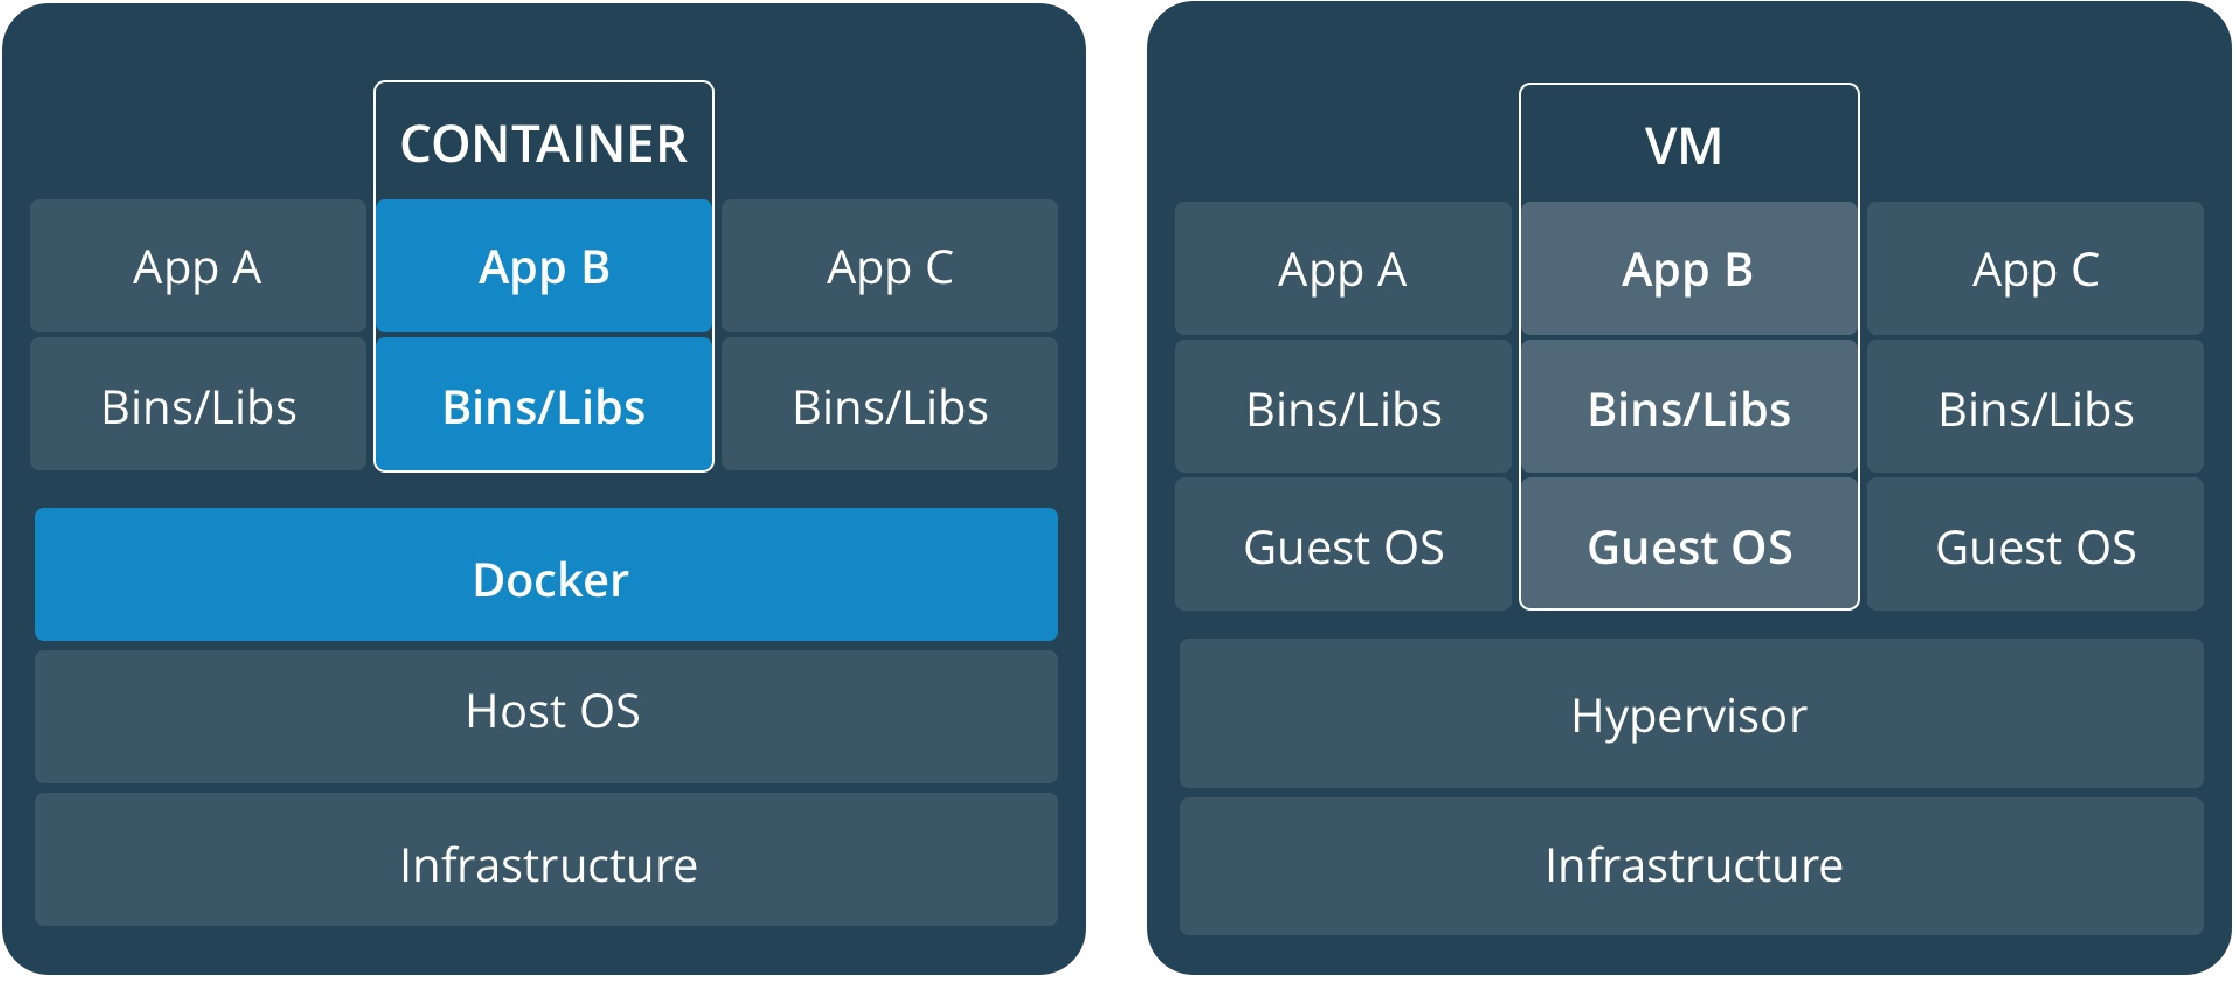
\includegraphics[width=0.8\textwidth]{chapter-background/containervsvm.pdf}
\end{figure}
\subsubsection{Docker}
Recently, thanks to Docker~\cite{dockersite}, containers have gained popularity and have been adopted into the software development process. However, Docker is not a new container technology, at its core it employs the kernel-level mechanisms of Linux containers (LXC), for which it defines a unified API~\cite{merkel2014docker}. In addition, the open-source Docker project offers a commandline-interface and daemon that offers easy packaging of applications in containers and the deployment of these containers.\\\\
To achieve this Docker introduces the concept of images. A container is represented by a lightweight image. A container image is a lightweight, executable package containing an application and its dependencies (runtime, libraries, environment variables, and config files). Virtual machines (VMs) can be seen as full, monolithic images. In particular,  Docker image consists of file-system layers stacked upon each other, as illustrated in Figure~\ref{docker-layers}. Only the top layer, the container itself, is writable, therefore it is state-full and executable. A container is thus composed out of layers of individual images built on top of a base image, allowing for easy extensibility.~\cite{pahl2015containerization} \\\\
A Docker image is specified by and build from a DockerFile. Images can be made easily accessible through Docker registries such as Dockerhub.\\
These images allow for easy and fast deployment of Docker containers across different operating systems and cloud provider stacks. Resulting in a game-changing technology for DevOps, system administrators and developers.
\begin{figure}[H]
\caption{Architecture of a container image. Images can be stacked upon each other using the cgroups and namespace extensions of a Linux kernel. The top container image is writable.~\cite{pahl2015containerization} \label{docker-layers}}
\centering
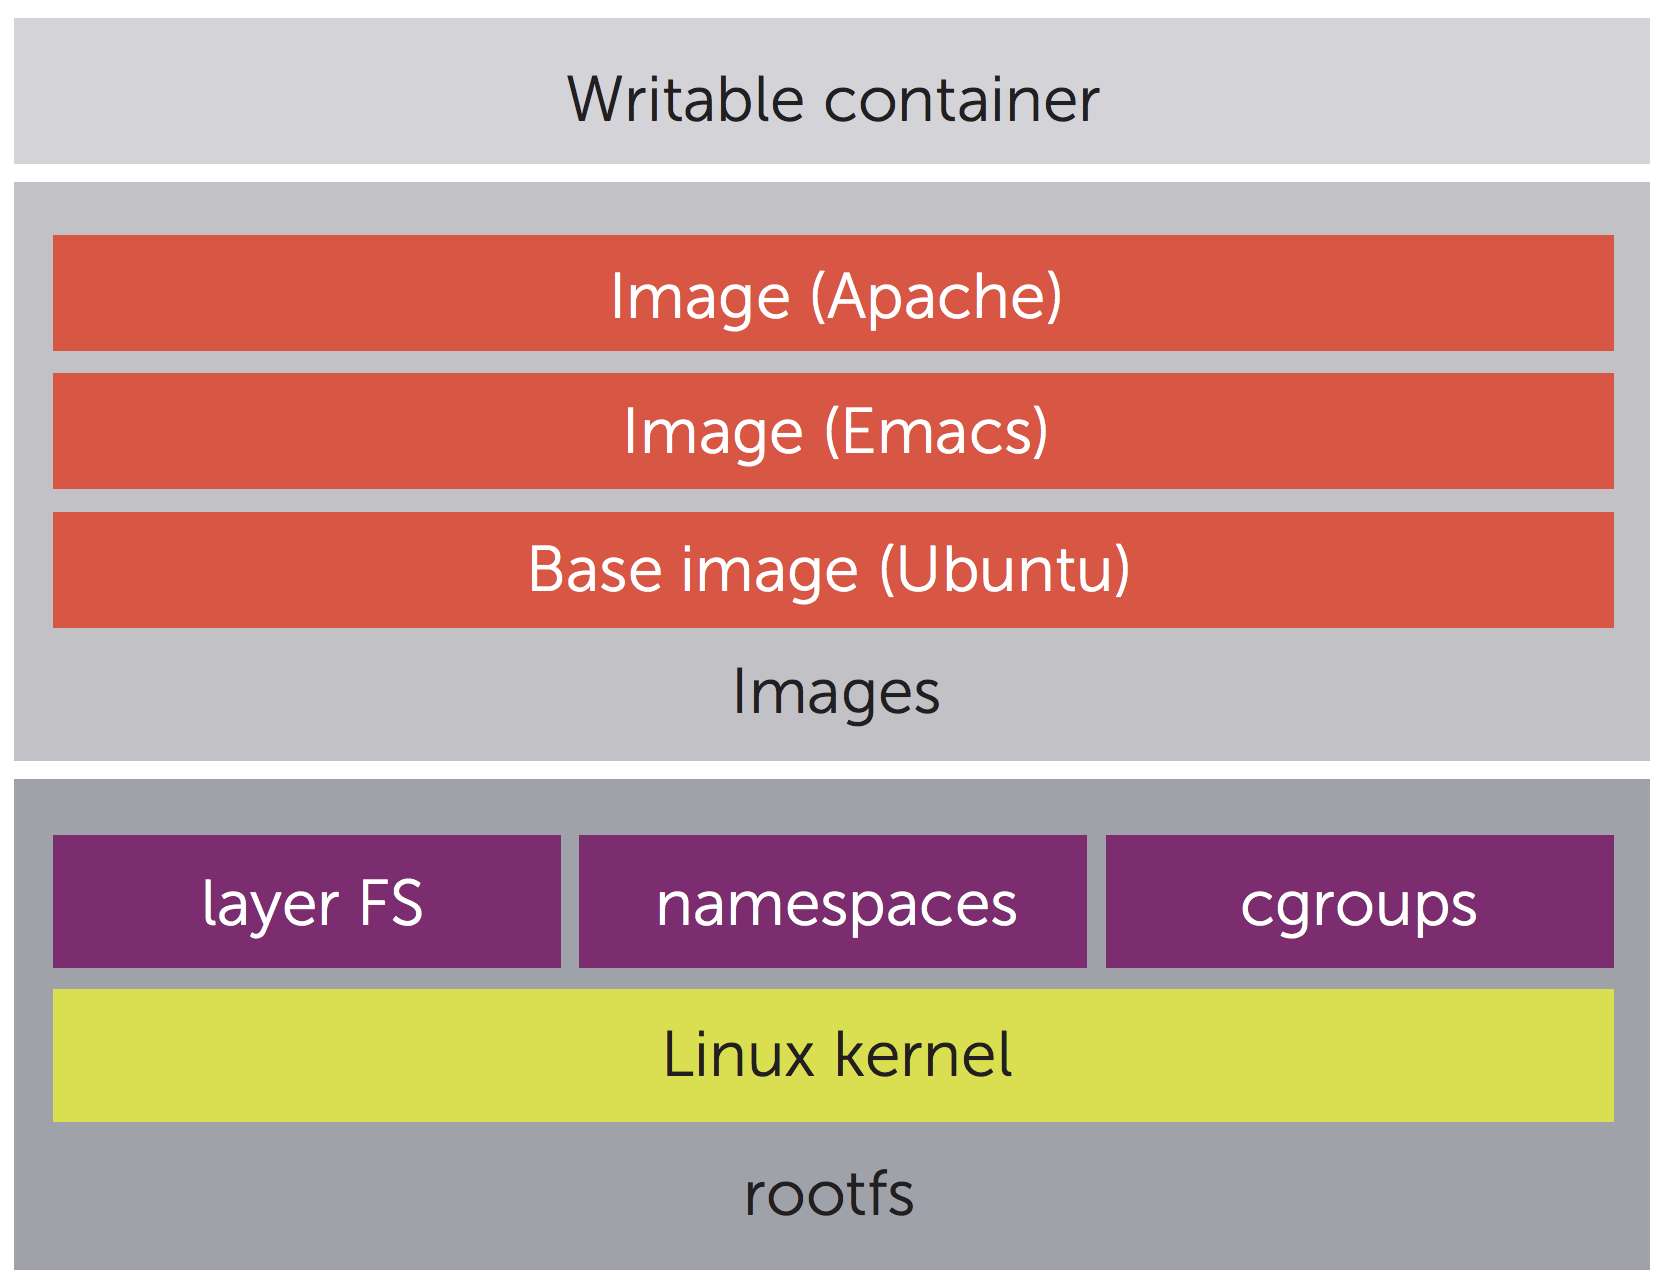
\includegraphics[width=0.5\textwidth]{chapter-background/docker-layers.png}
\end{figure}

\section{Container Orchestration}
Container technologies such as Docker offer advanced features to use containers in production. These solutions often offer deployment of applications limited to single machines. However, applications offered by  SaaS providers may include multiple different containers working together running on a cluster of nodes. Container orchestration (CO) systems allow deployment and management of containers at scale. Popular orchestration engines are Kubernetes, Docker Swarm and Mesos Marathon.
\subsection{Key capabilities of a container orchestration platform}
The task of a container orchestration (CO) platform is not limited to the initial deployment but the entire life-cycle of multiple containers. The goal of CO is to simplify cluster management while ensuring fault tolerance, availability, scalability and reliability. Allowing users to benefit from the complete potential of containers. In order to meet this goal, CO platform must at least offer the following key capabilities.~\cite{khan2017key}
\paragraph{Cluster state management and scheduling}
A cluster can be composed out of multiple virtualized or physical instances. Running containers on top of these instances and recover from failures requires a stable cluster. State management encapsulates various tasks such as flexible scheduling, re-partitioning of resources and data and propagating of dependent system changes.~\cite{khan2017key} 
\paragraph{High availability and fault tolerance}
A container orchestration platform must ensure high availability and fault tolerance in order to be useful for application developers. Most platforms therefor employ design principles of reliability engineering e.g., single point of failure elimination, failure detection or load balancing.~\cite{khan2017key}
\paragraph{Security}
Containers executing on top of the platform essentially form untrusted entities, with potentially malicious intentions, a high security standard is required. The standard should include: container images sanity check policies, access control for both containers and users, and techniques to minimize the container attack surface.~\cite{khan2017key}  
\paragraph{Simplified networking}
Containers must be able to communicate across nodes in  an efficient and secure manner. This requires the mapping of allocated host ports to containers. The overhead corresponding to this mapping intensifies at scale. The CO platform should thus provide a flexible, secure and scalable solution for networking.~\cite{khan2017key}
\paragraph{Service discovery}
The large number of services present in a cluster need to be able to communicate with each other. In traditional clusters services were handled as pets (i.e, having static names, IP addresses), however, in dynamic environments such as container orchestration platforms, they are regarded as cattle. The CO platform must provide mechanisms for addressing/labeling/grouping and service discovery.~\cite{khan2017key} 
\paragraph{Monitoring and governance}
The container orchestration platform needs to support traditional monitoring techniques such as logging, resource usage and network trace-routes. Monitoring must be possible at both the level of the underlying infrastructure and the containers themselves.~\cite{khan2017key}
\paragraph{Integrating for continuous integration and delivery}
Software development teams should be able to integrate the CO platform within their employed continuous integration and delivery (CI/CD) pipeline. The CO platform should contain mechanisms for rolling updates, rollbacks, etc.~\cite{khan2017key}


\subsection{Kubernetes}
Kubernetes~\cite{kubernetes}, commonly referred to as K8,  is one of the most popular and adopted orchestration systems. It is an open-source project led by Google. Kubernetes is Google's solution for the growing demand of container deployments by external developers in its public business cloud and is based upon its predecessors  Borg~\cite{verma2015large} and Omega~\cite{schwarzkopf2013omega} that have been used to schedule the internal Google workload. Its main design goal is formulated as:\textit{ "to make it easy to deploy and manage complex distributed systems, while still benefiting from the improved utilization that containers enable~\cite{Burns:2016:BOK:2930840.2890784}"}.  \\\\
\noindent To achieve the above stated goal Kubernetes introduces a number of concepts for both containers and cluster resources. It implements the infrastructure as code model  by provides an abstraction layer on top of the physical infrastructure~\cite{hermanns2015current}. It allows to setup and manage container infrastructure by the configuration of these introduced concepts via a REST API or declarative YAML configuration files. Below the most relevant concepts are introduced.
\subsubsection{Kubernetes concepts}
\textbf{Pods.}  A pod is the smallest unit of deployment within Kubernetes. It is a group of one or more containers that logically belong together.   A pod and thus its containers run on the same node. They share the same network, storage and context (Linux namespaces, cgroups). A pod gets assigned a unique IP address. Pods are not self-healing meaning when an error occurs within the pod or during scheduling. It will be deleted. Due to this short life cycle using a single pod resource and its assigned IP address for applications is impractical. Kubernetes handles this by employing controllers and services.~\cite{pods}\\\\
\textbf{Deployments.}  A Deployment controller manages a pod or a ReplicaSet of pods. A ReplicaSet allows pods to be replicated across multiple nodes. A Deployment object is used to specify the desired state of pods (e.g. number of replica's). A deployment, in addition, allows for declarative updates. These updates can be used to change the number of container replicas of a ReplicaSet or to update a specific container image within the pod.  The Deployment controller changes the actual state to the desired state described by the update.~\cite{deployments}
\\\\
\textbf{Services.}  Services offer a solution for the short life cycle of pods (and their IP addresses). Services within Kubernetes offer a manner to expose a ReplicaSet of Pods via a unique name, stable IP address, network policy and ports. To determine which set of pods is targeted by a service, Kubernetes employs a Label selector. Labels are the core grouping primitive of Kubernetes and unlike names and UIDs do not offer uniqueness.\\  A Service can be exposed outside the cluster by using an external load balancer or by specifying a NodePort. When using a Nodeport each node within the cluster will expose the port and forward request into the service.~\cite{services}
\\\\
\textbf{Namespaces.}  Namespaces allow to partition resources of a physical cluster among multiple user organizations. Each namespace gets a share of the resources of the cluster, via resource quotas. Resource quotas are supported for CPU, memory and persistent volumes.~\cite{namespaces-k8}
\\\\
\textbf{Resource limits.}  Kubernetes allows the allocation of compute resources of both containers and Namespaces by the means of resource limits. These limits can be soft (limit) and hard (request) limits. A Request specifies the quantity of resource that is guaranteed to the container. A limit specifies the maximum quantity allocated to the container. When the requested resource quantities of a container are less than its limit, the container may be allocated additional resources if there are unallocated resources available.  The current supported compute resources are CPU, memory and storage within the root partition of the local node. Within a Pod it is possible to specify both request and limit for each container. When request and limits are specified, the scheduler will use them for both scheduling and eviction (when node capacity is reached) decisions.~\cite{kubresources}
\subsubsection{Kubernetes architecture}
The basic architecture of Kubernetes is illustrated in Figure~\ref{fig:kubarch}. A client-server architecture is employed in which master and node setups are deployed on different machines. Below the different components that build up the architecture are briefly explained. 
\paragraph{API Server.} The API server is responsible for the configuration and validation of API objects (pods, deployments, services,...). It offers communication on cluster state via a REST interface for both components and administrators.~\cite{kubernetes-api-server}
\paragraph{Controller manager.} The controller manager is responsible for managing several core control loops part of Kubernetes. A control loop uses the API server to observe the shared state of the cluster and attempts to move to the desired state via configuration changes.~\cite{kubernetes-controller-manager}
\paragraph{Scheduler.} The task of assigning pods to nodes is the responsibility of the scheduler component.  The scheduler attempts to do a reasonable placement based on resource and quality of service requirements (e.g., not place a pod on a node with insufficient resources). It is  possible for users to control the placement of pods via NodeSelector tags or affinity and anti-affinity constraints in the configuration file.~\cite{kubernetes-pods-to-nodes,kubernetes-scheduler}
\\\\In addition it is possible to assign Quality of Service (QoS) classes to pods. These are used by Kubernetes in the decision process about scheduling and eviction of pods. Currently, Kubernetes supports three types of classes: guaranteed, burstable and best-effort. In decreasing order of priority (i.e., most likely to be killed in the case of resource shortages). The QoS classes are assigned to pods based on the presence of request and limit specifications of resources in their configuration files.~\cite{kubernetes-qos}


\paragraph{Kubelet.} The kubelet component is an agent running on each node. It is responsible for running and maintaining pods on its residing node. The set of maintained pods is described in the form of PodSpecs (mainly received via the API-server).~\cite{kubernetes-kubelet}
\paragraph{Kube-proxy.} The kube-proxy daemon provides a simple network proxy for the services on each node. It enables forwarding of requests to the correct containers and can provide primitive load balancing.~\cite{kubernetes-kubeproxy}
\begin{figure}[H]
\caption{Kubernetes architecture}
\centering
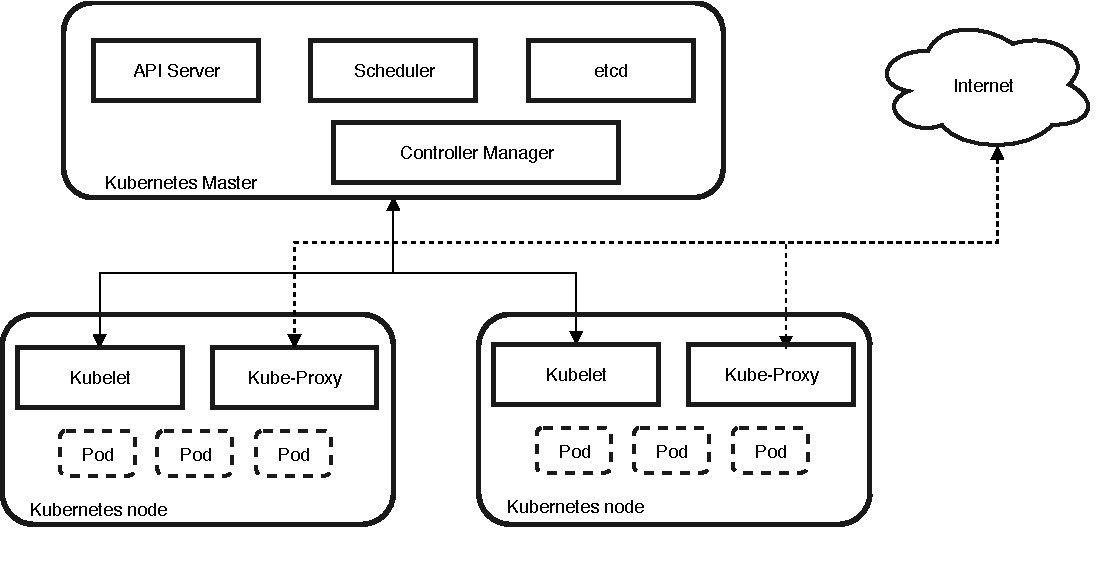
\includegraphics[width=0.8\textwidth]{chapter-background/kubernetes-architecture-diagram.pdf}
\label{fig:kubarch}
\end{figure}
 
 
 
 
 
 
 
 
 
 \section{Performance evaluation}
As discussed in previous sections, SaaS providers employ multi-tenancy to improve  cost efficiency and offer several performance guarantees to their customers in the form of SLOs. An unavoidable consequence of multi-tenancy is the need to support a growing number of users in a single system. Providers need to have a clear insight into the \textit{scalability} of their systems. However, scalability is a difficult thing to define, let alone quantify. Citing the words of  Dr. Neil J. Gunther:  \textit{"if you can't quantify it, you can't guarantee it"}.~\cite{perfdynamics}

\subsection{The Universal Scalability Law}
\label{section-USL}
Dr. Neil J. Gunther provides a formal definition of scalability: \textit{"scalability can be defined as a mathematical function, a relationship between independent and dependent variables (input and output)"~\cite{perfdynamics}}. The Universal Scalability Law (USL) by Dr. Neil J. Gunther is presented in Equation~\ref{USL}. It computes the relative capacity $C(N)$ at a load of $N$ users. Relative capacity is the normalized throughput.
\begin{equation}
\label{USL}
C(N) = \frac{\gamma~N}{1 + \alpha~(N-1) + \beta~N~(N-1)}
\end{equation}

The Universal Scalability Law incorporates factors that contribute to the sublinearly scalability of most systems. Namely, \textbf{concurrency} ($\gamma$), \textbf{contention} ($\alpha$) and \textbf{coherency} ($\beta$) as explained below. Their impact is visualized in Figure~\ref{fig:usl-impact}.

\begin{itemize}
    \item \textbf{Concurrency}($\gamma$): $\gamma$ defines the slope if the system was linearly scaling i.e., $C(N) = \gamma N$. It has been referred to as the \textit{coefficient of performance} by~\cite{schwarz2015practical}.
    \item \textbf{Contention} ($ \alpha $) : When scaling most systems parallelism while be limited at some point by contention (i.e., waiting or queuing for shared resources). The maximum speedup by parallelism is limited by the serialized portion ($\alpha$) of the work~\cite{schwarz2015practical}. 
    \item \textbf{Coherency} ($\beta$): created by crosstalk between components. Because crosstalk is possible between each pair of components in the system, the penalty grows quadratic $N(N-1)$.~\cite{schwarz2015practical}
    
\end{itemize}

\begin{figure}
    \centering
    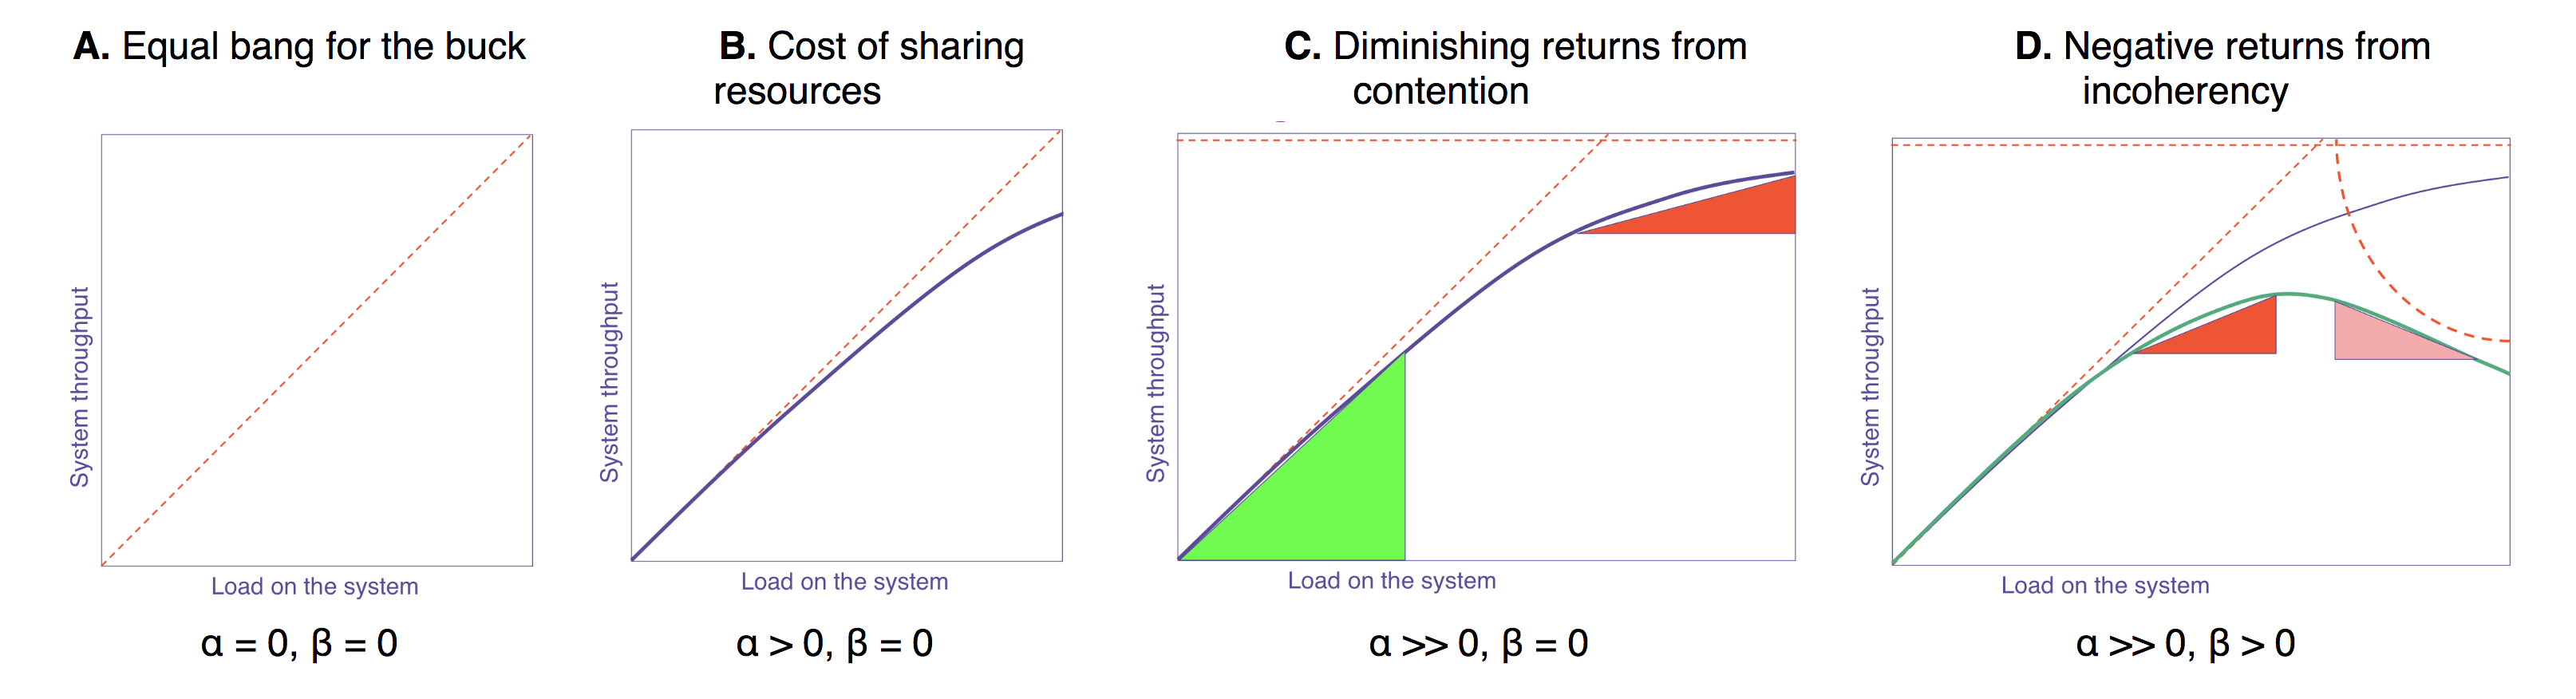
\includegraphics[width=1.1\textwidth]{chapter-evaluation/usl-impact}
    \caption{The impact of different USL coefficients on scalability.~\cite{perfdynamics}}
    \label{fig:usl-impact}
\end{figure}

\subsubsection{USL in practice}
USL can provide insights into a system's scalability pains via  values of the concurrency, contention and coherency coefficients. These can be obtained by collecting a dataset of measurements of the system, system load $N$ and corresponding throughput, and using a statistical technique such as nonlinear least square regression which fits the USL to the dataset.~\cite{schwarz2015practical,heyman2014scalability}

\subsection{Little's law}
\label{sec:little}
The Universal Law of Scalability serves as an alternative for the often less intuitive queuing models frequently used for modeling scalability. It omits the need to know the service time for every queue in the performance model in order to predict the response time or latency~\cite{perfdynamics}. Nevertheless, queuing theorem and its lemmas such as Little's Law can provide useful insights into performance modeling.\\\\
John D.C Little's Law~\cite{little2008little} states the following for stable systems: 
\begin{displayquote}
\textit{"The average number of items in a queuing system equals the average rate at which items arrive multiplied by the average time that an item spends in the system.\cite{little2008little}"}
\end{displayquote}
\begin{equation}
\label{littleslaw}
L = \lambda~W
\end{equation}
\begin{equation}
\label{llsys}
N = X~Rt
\end{equation}
Equation~\ref{littleslaw} shows Little's law, below its terms and its applicability to web services (Equation~\ref{llsys}) are explained:
\begin{itemize}
    \item \textbf{$L$}:  Average number of items in the system. For a web service this is represented by the average number of concurrent users in the system $N$.
    \item \textbf{$\lambda$}: Long-term average arrival rate of items in the system per time unit. Little's law assumes a stable system for which the arrival rate and exit rate are identical. In a web service this is represented by the throughput $X$.
    \item \textbf{$W$}: Average waiting time of an item in the system, queuing time and service time combined. This is represented by the response time $Rt$ or latency of a request in a web service. When dealing with a system involving think time (e.g., after the response from a web service, a user needs time to think about his/her next request), $(Rt + Zt)$ is used. 
\end{itemize}

\subsubsection{Workload generator validation}
Developers employ software tools (JMeter~\cite{jmeter}, Locust~\cite{locust}, etc.)  to simulate a workload and test the performance of a system. A workload is a set of actions that represent the behavior of a client in the system. It is part of the test plan stating the number of concurrent users $N$ executing the workload for a specified period of time.\\\\
The results of a performance test are typically expressed in throughput $X$ and response time $Rt$. Using Little's law it is possible to validate these results. For example, a test plan of 1000 concurrent users $N$ results in a throughput of 50 requests per second and an average response time of 15 seconds. Following Little's law, a concurrence of only 750 users was reached, instead of the specified 1000. Little's law can thus be used to check if a workload generator works as specified.\\\\
Alternatively, if the average throughput and response time for a production system are known, Little's law can be used to correctly draw up a test plan.

\subsubsection{Response time or latency?}
Performance can either be measured in throughput or latency, both are correct but offer a different point of view. System performance is typically expressed in throughput: "The system can handle a million operations per second". However, users care more about their personal experience with a system which is influenced by the average latency of their request.~\cite{schwarz2015practical} \\\\
Figure~\ref{fig:ls_vs_tp} shows the relation between the average latency and throughput of a database under increasing load $N$. In this case, latency is kept stable by increasing the throughput with the increasing load up to a certain point.  A bottleneck caps the throughput of the systems and by Little's law for an increasing load and constant throughput, the latency must increase.~\cite{latvsthrough} \\\\
However in other systems, as discussed in Section~\ref{section-USL}, an increasing load might induce a diminishing result on the system's throughput. Following Little's law a decreasing throughput results in a higher latency under the same load. \\\\
Thus, for stable systems by Little's law,  the USL can be reformulated in terms of latency instead of throughput. Equation~\ref{USL-2} shows this reformulation.~\cite{schwarz2015practical}
\begin{equation}
\label{USL-2}
Latency(N) = \frac{1 + \alpha~(N-1) + \beta~N~(N-1)}{\gamma}
\end{equation}


\begin{figure}[H]
    \centering
    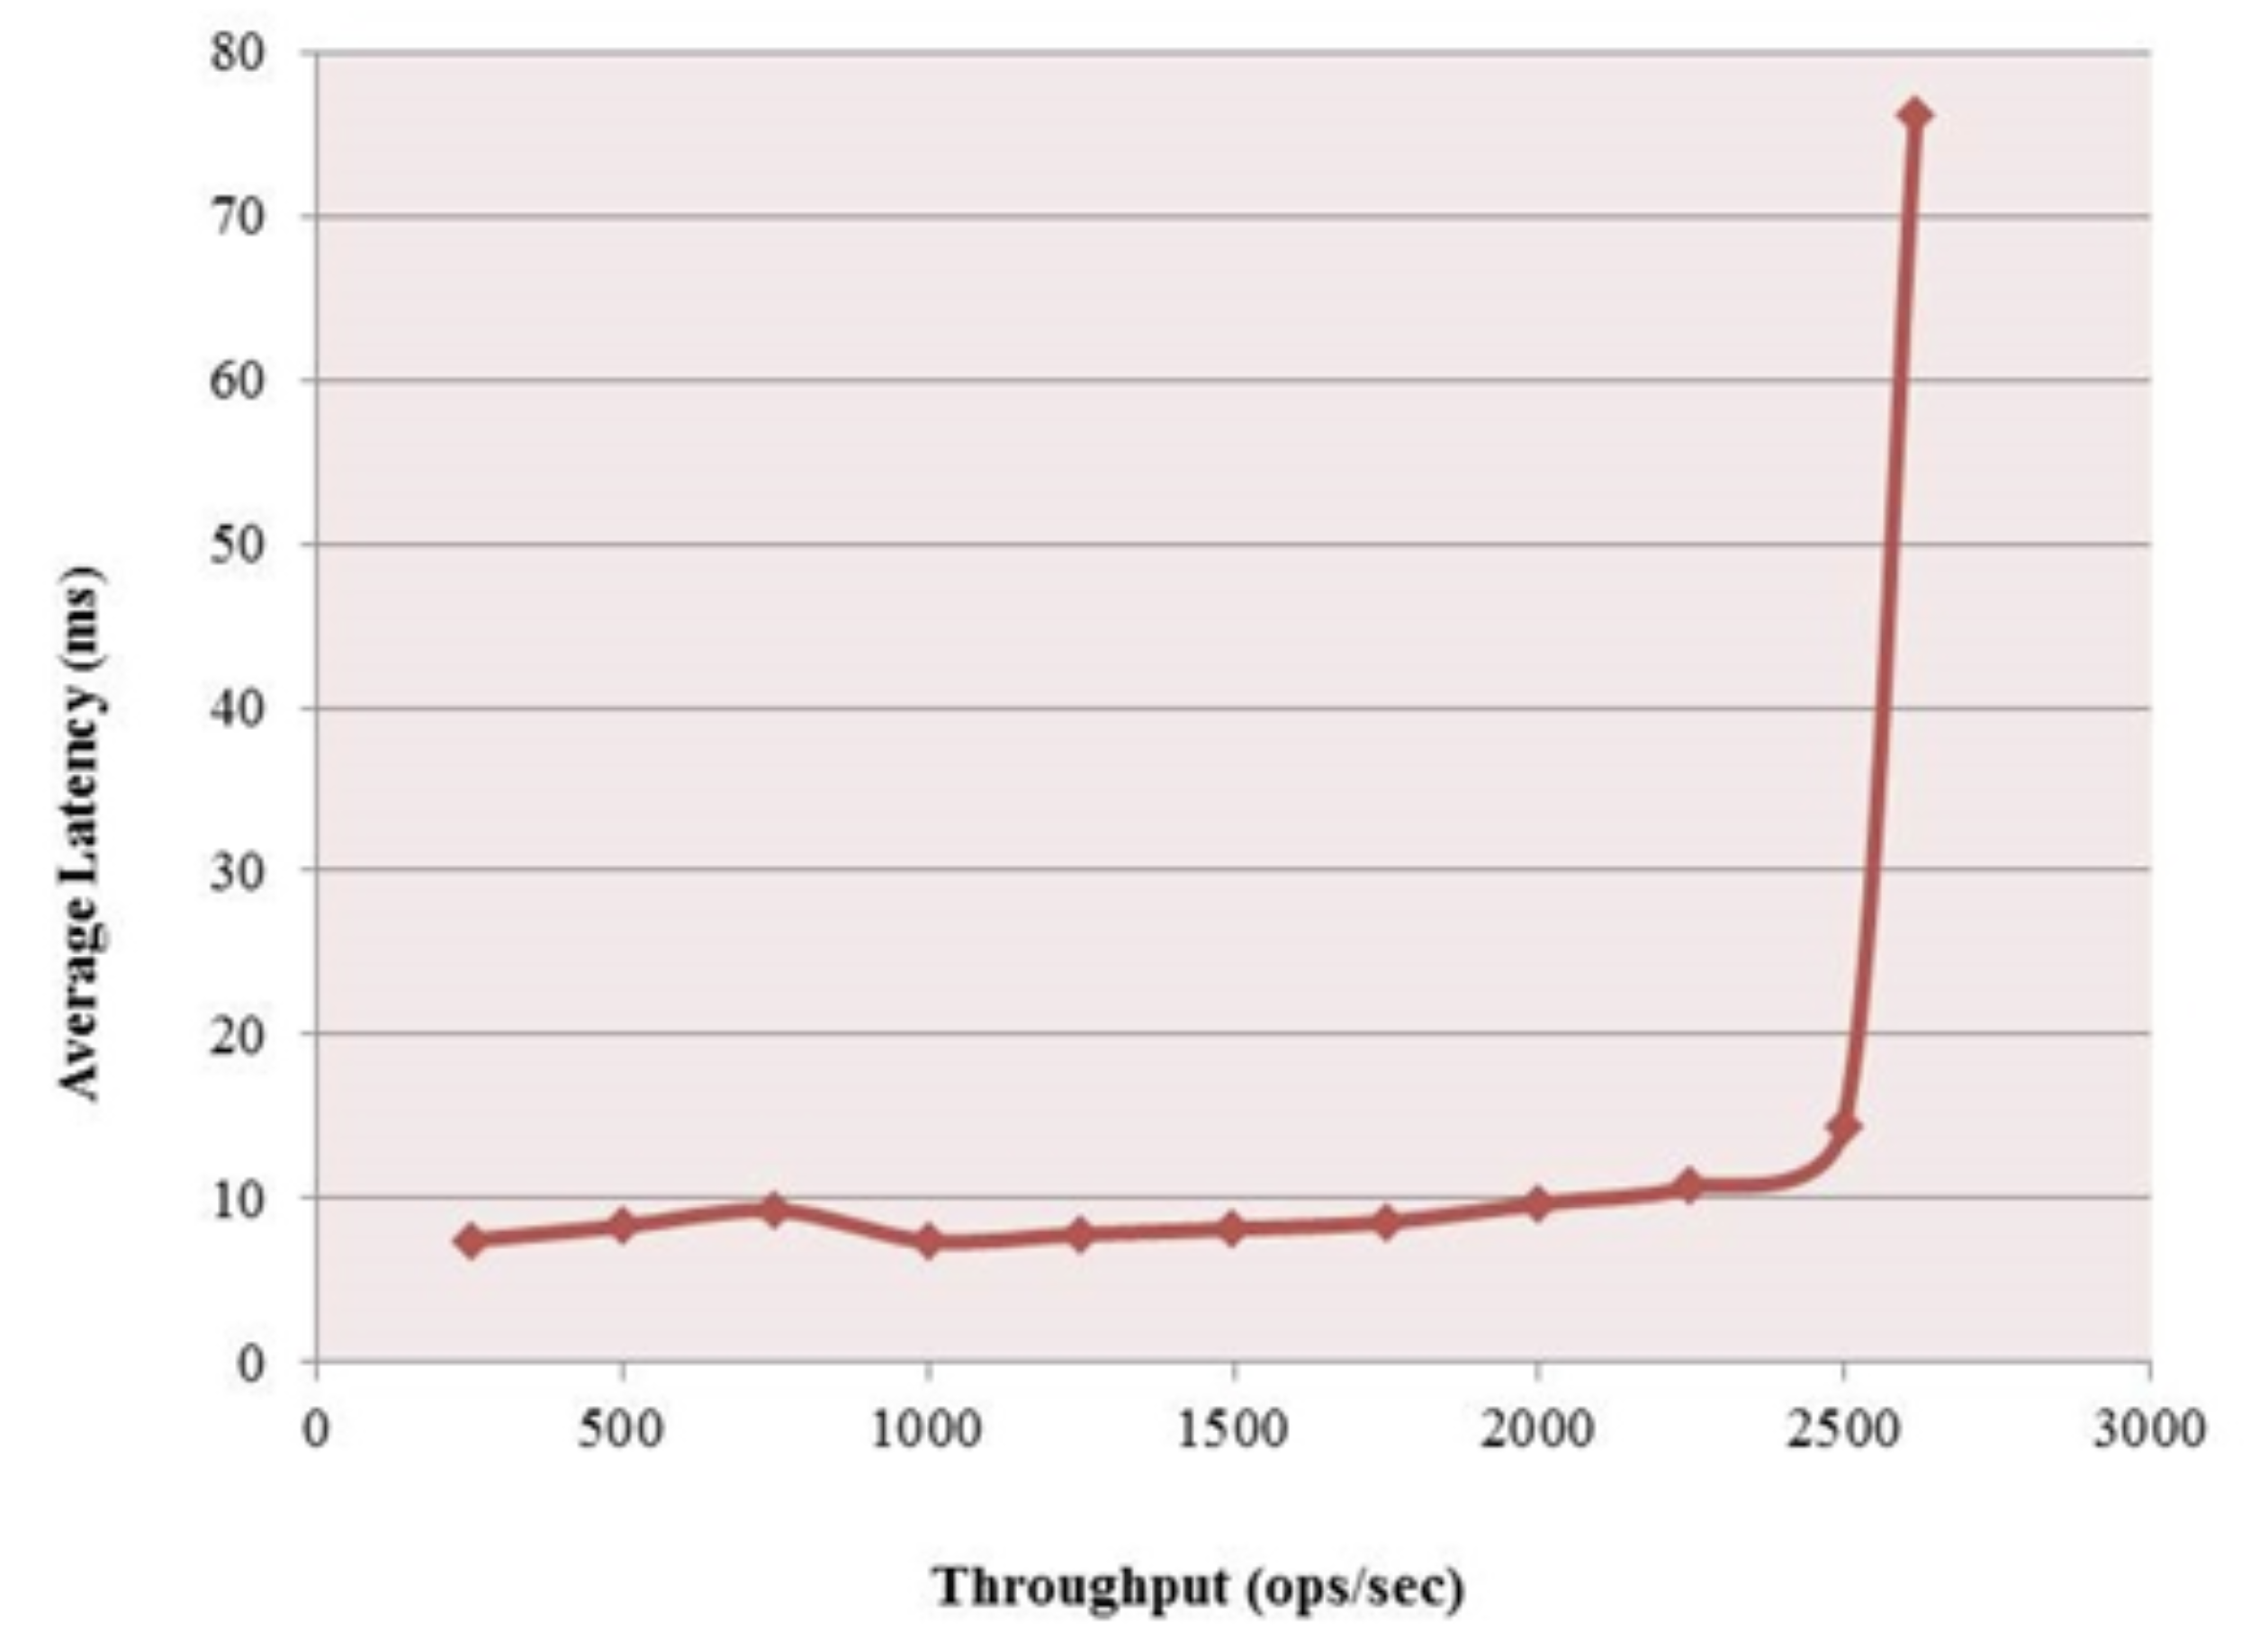
\includegraphics[width=0.8\textwidth]{chapter-evaluation/ls_vs_th}
    \caption{Relation average latency vs. throughput for database benchmark with increasing load.~\cite{latvsthrough}}
    \label{fig:ls_vs_tp}
\end{figure}
\chapter{Background}
\label{ch:background}
This chapter discusses relevant background material for the thesis. The concepts, explored in this chapter, further clarify the relevance of the thesis and serve as building blocks for the remaining chapters. Starting from the adoption of the cloud computing paradigm, the chapter elaborates on how concepts such as multi-tenancy and virtualization via containerization push the limits of efficient resource utilization. Next, an in-depth overview of the open-source container orchestration platform Kubernetes is provided. Lastly, insights are provided into the universal scalability law and the applicability of Little's law for performance testing.
\section{Cloud computing}
Companies try to minimize the total cost of ownership by moving to cloud computing or utility computing. The cloud computing paradigm enables on-demand access to a shared pool of configurable compute resources (software applications, system software and hardware infrastructure)~\cite{WalravenStefan2015PPmf}. A service provider can provision the required resources from the cloud with minimal effort.  Within this paradigm, services are offered in real time over the internet in three different models~\cite{MellPeter2010TNDo,rimal2009taxonomy}. 
\begin{itemize}
\item \textit{Infrastructure as a Service (IaaS)} in which access is offered to virtual machines, network, data storage and other fundamental computing resources. The customer is able to deploy arbitrary software using these resources.\\\\
Examples: Digital Ocean, Microsoft Azure and Amazon Elastic Compute Cloud (EC2).
\item \textit{Platform as a service (PaaS)} offers customers a platform enabling easy and efficient deployment of applications (at scale) while abstracting the complexity of managing the underlying infrastructure. PaaS allows customers to solely focus on the development of their application.\\\\
Examples: Google app engine, Microsoft Azure and Heroku.
\item \textit{Software as a service (SaaS) } allows customers to make use of a specific application developed by a SaaS provider. Compared to the traditional use of software, the management and deployment is the task of the SaaS provider. In this strategy, common resources and a single instance of both the application and underlying database are used to support multiple customers simultaneously. \\\\
Examples: Google apps and Salesforce.
\end{itemize}

\section{Multi-tenancy}
\label{multi-tenancy}
The software as a service (SaaS) model offers applications to customers as an on-demand service. Providers of these applications try to leverage economies of scale by employing a multi-tenancy architectural design principle. The goal of multi-tenancy is to minimize the total cost of ownership for the provider by maximizing the sharing of resources among multiple customers organizations, referred to as tenants.~\cite{Walraven2015b} 
\subsection{Service Level Agreements}
By moving their core business functions to an entrusted cloud provider, cloud customers give up control of the underlying compute resources. It is vital for these tenants to obtain certain guarantees on the service delivered by the provider. 
A Service Level Agreement (SLA) is a formal contract between the SaaS provider and the tenant specifying both properties of the provided service and the expected behavior of the tenant. An SLA typically also contains a set of Service Level Objectives (SLOs). An SLO is a measurable characteristic of the service. An SLO is typically related to performance constraints (latency, throughput and deadlines) or availability (uptime percentage) of the service. Within the specification of an SLA a trade-off must often be made between expressiveness and usability. The SLA must cover all the expectations of a customer while remaining simple to weight, verify, evaluated and enforce~\cite{dillon2010cloud}.  Some typical examples of SLOs are shown below: 
\begin{itemize}
\item The application has a monthly uptime percentage of 99.95\%.
\item If the arrival rate of the tenant workload < X requests/s then a throughput T is guaranteed.
\end{itemize}
\subsection{Challenges}
While the goal of multi-tenancy is promising, sharing a cluster of dynamically provisioned nodes between multiple tenants imposes a number of challenges and requirements~\cite{TruyenEddy2016Taca}. 
\begin{itemize}
\item Performance isolation: the activities of one tenant should not be able to influence the service level delivered to other tenants. This requirement should be achieved during normal system load and when an aggressive tenant violates the terms of the SLA. 
\item QoS differentiation: the performance guarantees specified by an SLA can be individually customized for each tenant. A SaaS provider should be able to offer different subscriptions.
\item Flexible resource allocation for improved server consolidation: a SaaS provider employs a multi-tenant architecture to achieve a lower operational cost. This is partially achieved by planning the required node capacity based on the actual resource usage of tenants instead of the theoretical required capacity.  This can be further aided by the use of request schedulers allowing to distinguish between normal, passive and aggressive tenants. 
\end{itemize}
\subsection{Strategies}
To achieve multi-tenancy different strategies, each offering different trade-offs concerning operational costs and upfront application engineering costs, can be employed by the SaaS-provider~\cite{WalravenS.2011Amlf}. The strategies are illustrated in Figure~\ref{muti-tenant-strategies}.
\begin{itemize}
\item Multi-tenancy can be achieved at the level of the \textit{operating system}. In this strategy, a virtualization technology can be used to partition compute resources among multiple virtual machines. Each tenant is assigned an application instance running on a dedicated virtual machine. This approach offers both a higher level of performance isolation and lower upfront engineering costs but suffers from an inefficient utilization of resources.
\item In \textit{middleware-level multi-tenancy} a middleware platform is used to enable sharing compute resources between multiple tenants at the level of the operating system. An application instance is deployed on top of the middleware platform for each tenant. By not replicating the operating system for each tenant a higher level of cost efficiency can be achieved but an increased complexity in managing resources and  performance isolation is introduced. By tackling these problems at the level of the middleware a part of the engineering complexity is shifted to this level.
\item The most efficient resource utilization can be achieved by sharing application instances between multiple tenants. In \textit{Application-level} multi-tenancy achieving performance isolation is done by the application itself thereby increasing the engineering complexity and costs.
\end{itemize}


\begin{figure}[H]

\caption{Different strategies to achieve multi-tenancy~\cite{WalravenS.2011Amlf}.\label{muti-tenant-strategies} }
\centering
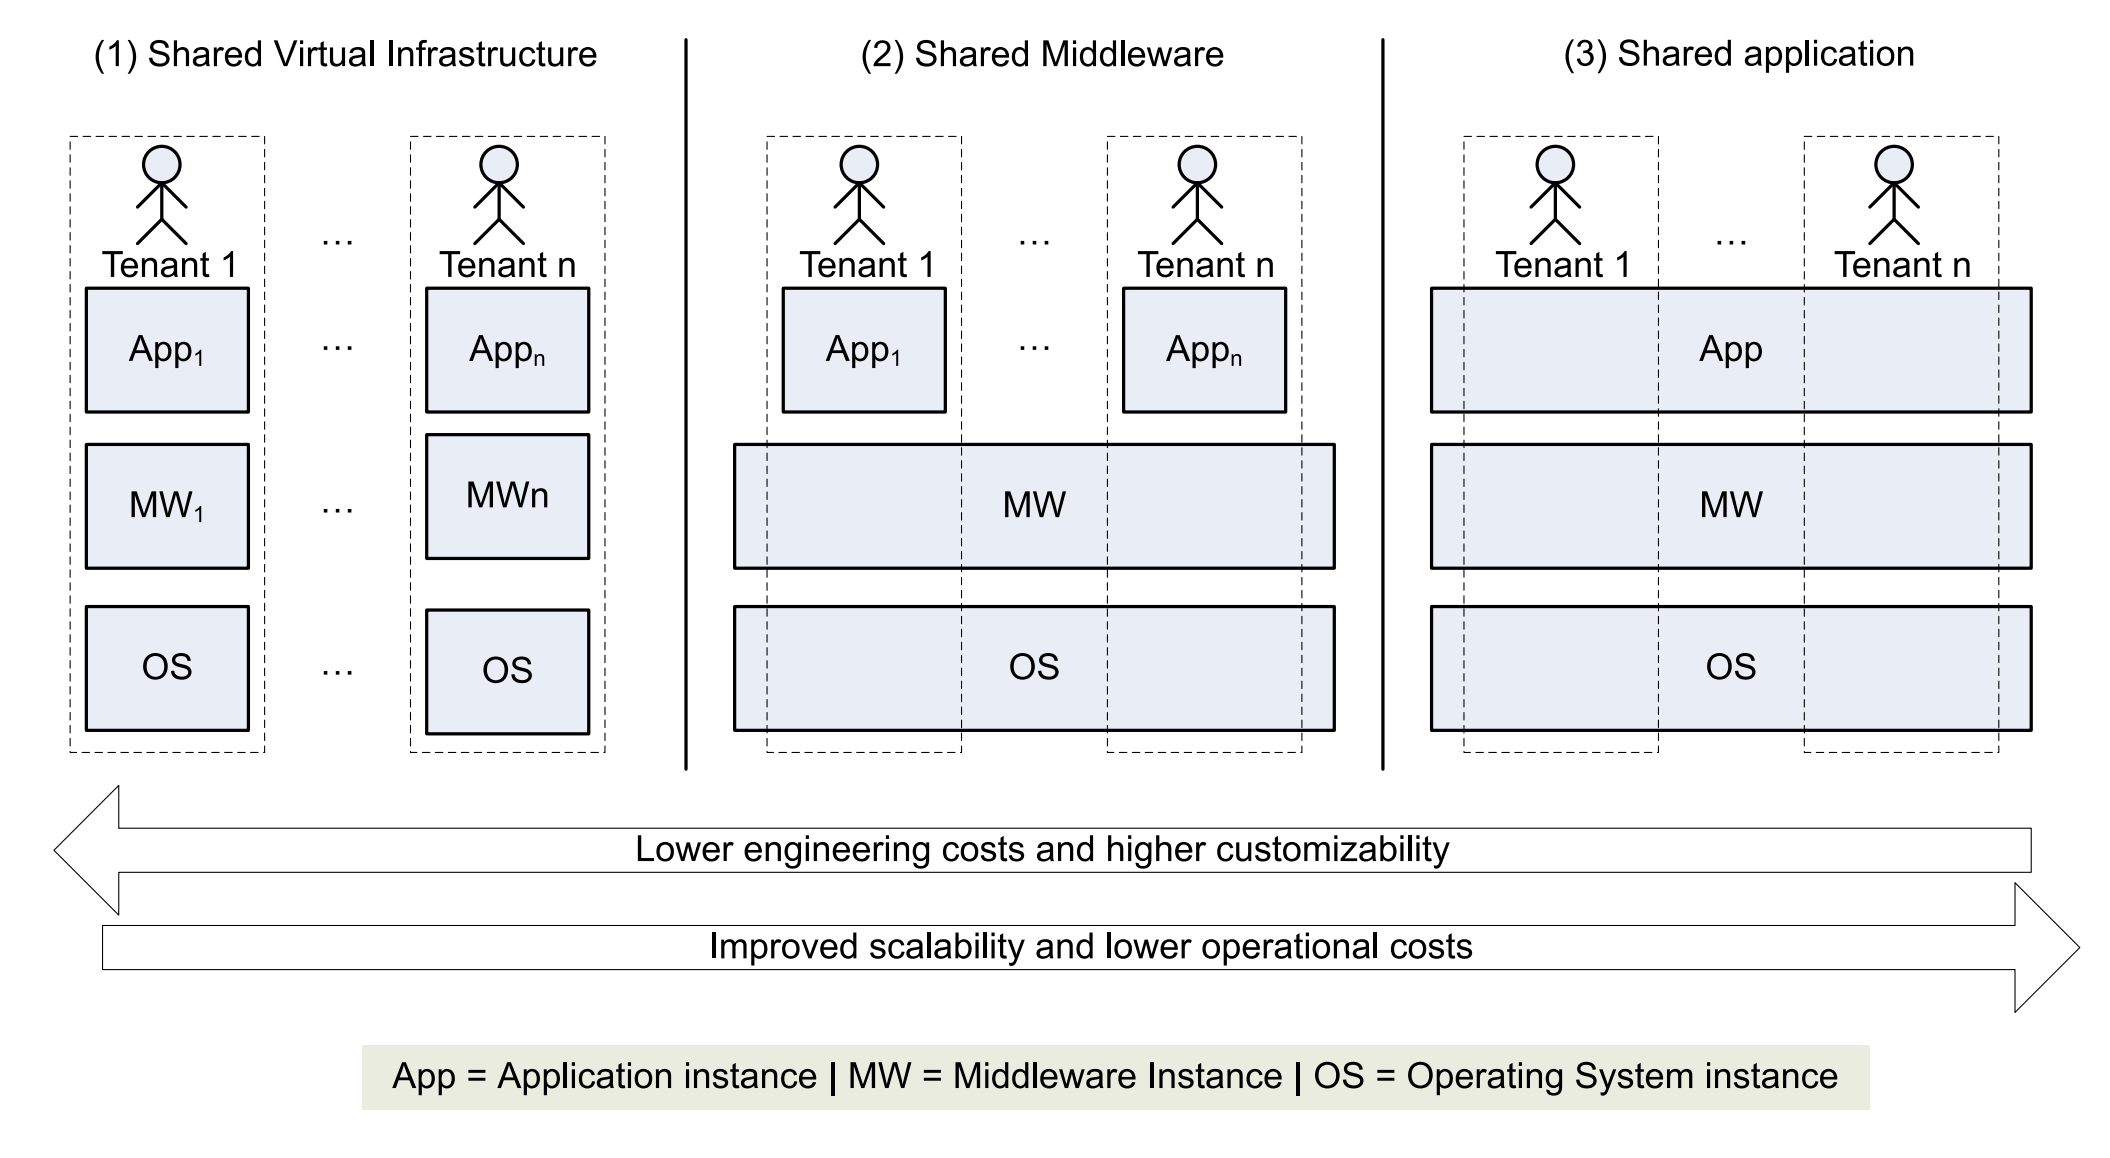
\includegraphics[width=0.65\textwidth]{chapter-background/muti-tenant-strategies.png}
\end{figure}


\section{Containerization}
Cloud providers rely on virtualization technology for the achievement of large-scale resource scaling. For more than a decade, virtual machines (VMs) have been the backbone of a provider's infrastructure offering hardware independence, availability, isolation and security~\cite{xavier2013performance}. More recently, containers a more lightweight virtualization technology have made advances in their multi-tenant capabilities and have seen an increase in adoption by providers~\cite{pahl2015containerization}. Both are discussed in this section.
\subsection{Virtualization technology}
In cloud environments, virtualization technology is used for flexible and dynamic allocation of physical resources to virtualized applications and to achieve multi-tenancy by sharing a physical server among multiple applications. In data centers virtualization is commonly used at the \textit{hardware level} and \textit{operating system level} to deploy and manage virtual machines and applications at scale~\cite{SharmaPrateek2016CaVM}. \\\\
Hardware level virtualization uses a hypervisor on a server to create virtual machines. Each virtual machine provides an abstraction of a physical machine and runs an independent operating system with applications. The hypervisor is responsible for resource allocation and performance isolation.\\\\
Operating system level virtualization allows resources to be shared at the level of the OS. Virtual machines running at the OS level are referred to as containers. Isolation, abstraction and resource allocation of containers is performed by the OS kernel of the host OS. By sharing the OS kernel among multiple containers, containers are regarded as a more lightweight virtualization technology. Containers only contain the application and its dependencies.\\\\
Linux containers (LXC)~\cite{lxc} employ different mechanisms of the Linux kernel to achieve resource isolation, namely control groups and namespaces.
\begin{itemize}
    \item \textbf{Cgroups}~\cite{cgroups} allow for fine-grained control of the allocation of system resources (CPU time, system memory, network bandwidth) among processes and process groups. For example, it is possible to limit or prioritize memory, CPU or I/O usage of different containers. 
    \item \textbf{Namespaces}~\cite{namespaces} allow for isolation of kernel resources among processes. A namespace makes a resource appear to be private and isolated for the container. The Linux kernel provides the following namespaces:  process ids, inter-process communication (IPC) mechanisms, network stack and mount points.
\end{itemize}
Linux containers (LXC) offers a lightweight implementation which performs at native speed and provides good isolation. However, while sharing a kernel between containers minimizes overhead, there are limitations in terms of the security environment.~\cite{dua2014virtualization}
\\\\
\noindent By offering virtualization at different levels, containers and VMs offer different trade-offs concerning performance isolation and performance. Research~\cite{SharmaPrateek2016CaVM} concludes that while containers offer closer to bare metal performance compared to VM, they offer worse performance isolation in multi-tenant environments. In addition, containers offer soft resource limits compared to the hard resource limits of virtual machines which allow for better server consolidation in over-commitment scenarios.  
\begin{figure}[h]
\caption{Container vs virtual machine.~\cite{container-vs-vms}}
\centering
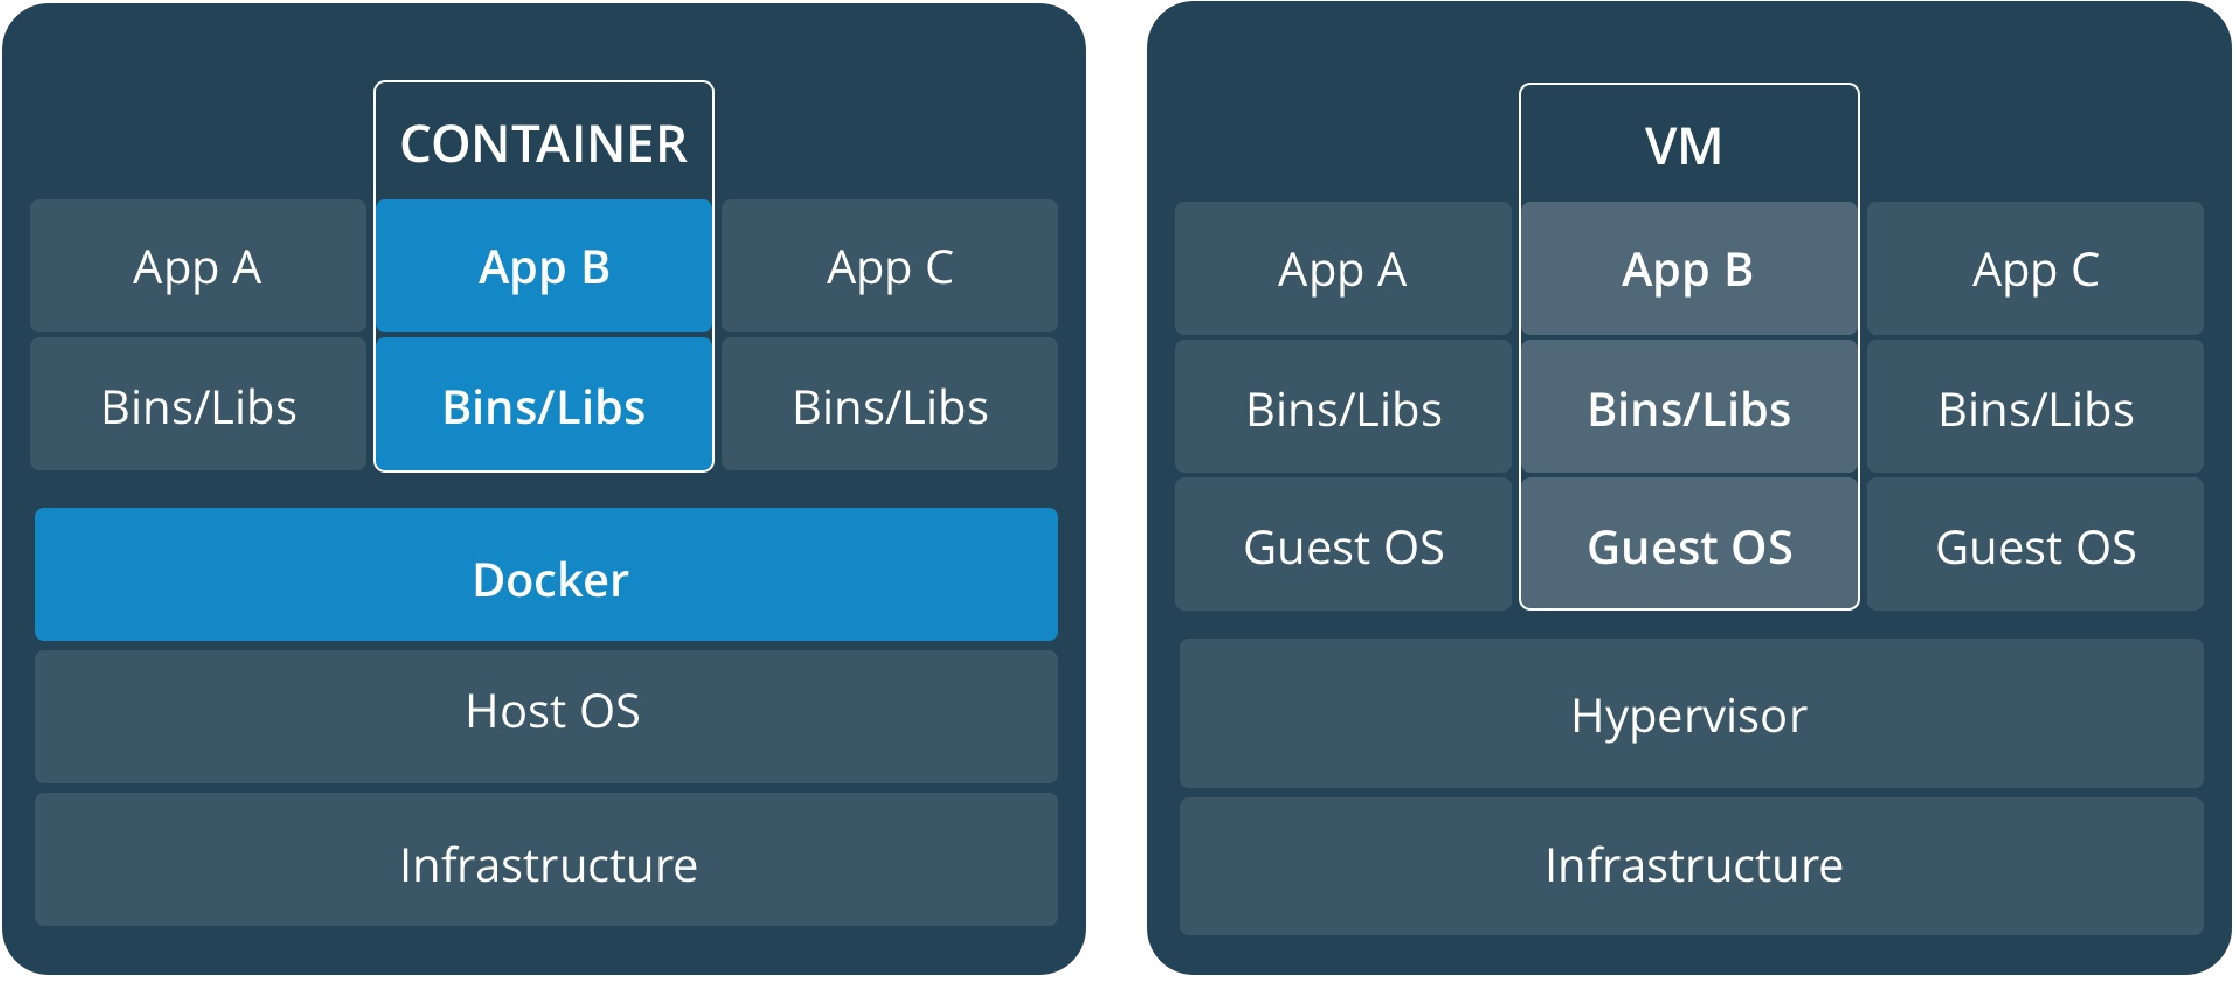
\includegraphics[width=0.8\textwidth]{chapter-background/containervsvm.pdf}
\end{figure}
\subsubsection{Docker}
Recently, thanks to Docker~\cite{dockersite}, containers have gained popularity and have been adopted into the software development process. However, Docker is not a new container technology, at its core it employs the kernel-level mechanisms of Linux containers (LXC), for which it defines a unified API~\cite{merkel2014docker}. In addition, the open-source Docker project offers a commandline-interface and daemon that offers easy packaging of applications in containers and the deployment of these containers.\\\\
To achieve this Docker introduces the concept of images. A container is represented by a lightweight image. A container image is a lightweight, executable package containing an application and its dependencies (runtime, libraries, environment variables, and config files). Virtual machines (VMs) can be seen as full, monolithic images. In particular,  Docker image consists of file-system layers stacked upon each other, as illustrated in Figure~\ref{docker-layers}. Only the top layer, the container itself, is writable, therefore it is state-full and executable. A container is thus composed out of layers of individual images built on top of a base image, allowing for easy extensibility.~\cite{pahl2015containerization} \\\\
A Docker image is specified by and build from a DockerFile. Images can be made easily accessible through Docker registries such as Dockerhub.\\
These images allow for easy and fast deployment of Docker containers across different operating systems and cloud provider stacks. Resulting in a game-changing technology for DevOps, system administrators and developers.
\begin{figure}[H]
\caption{Architecture of a container image. Images can be stacked upon each other using the cgroups and namespace extensions of a Linux kernel. The top container image is writable.~\cite{pahl2015containerization} \label{docker-layers}}
\centering
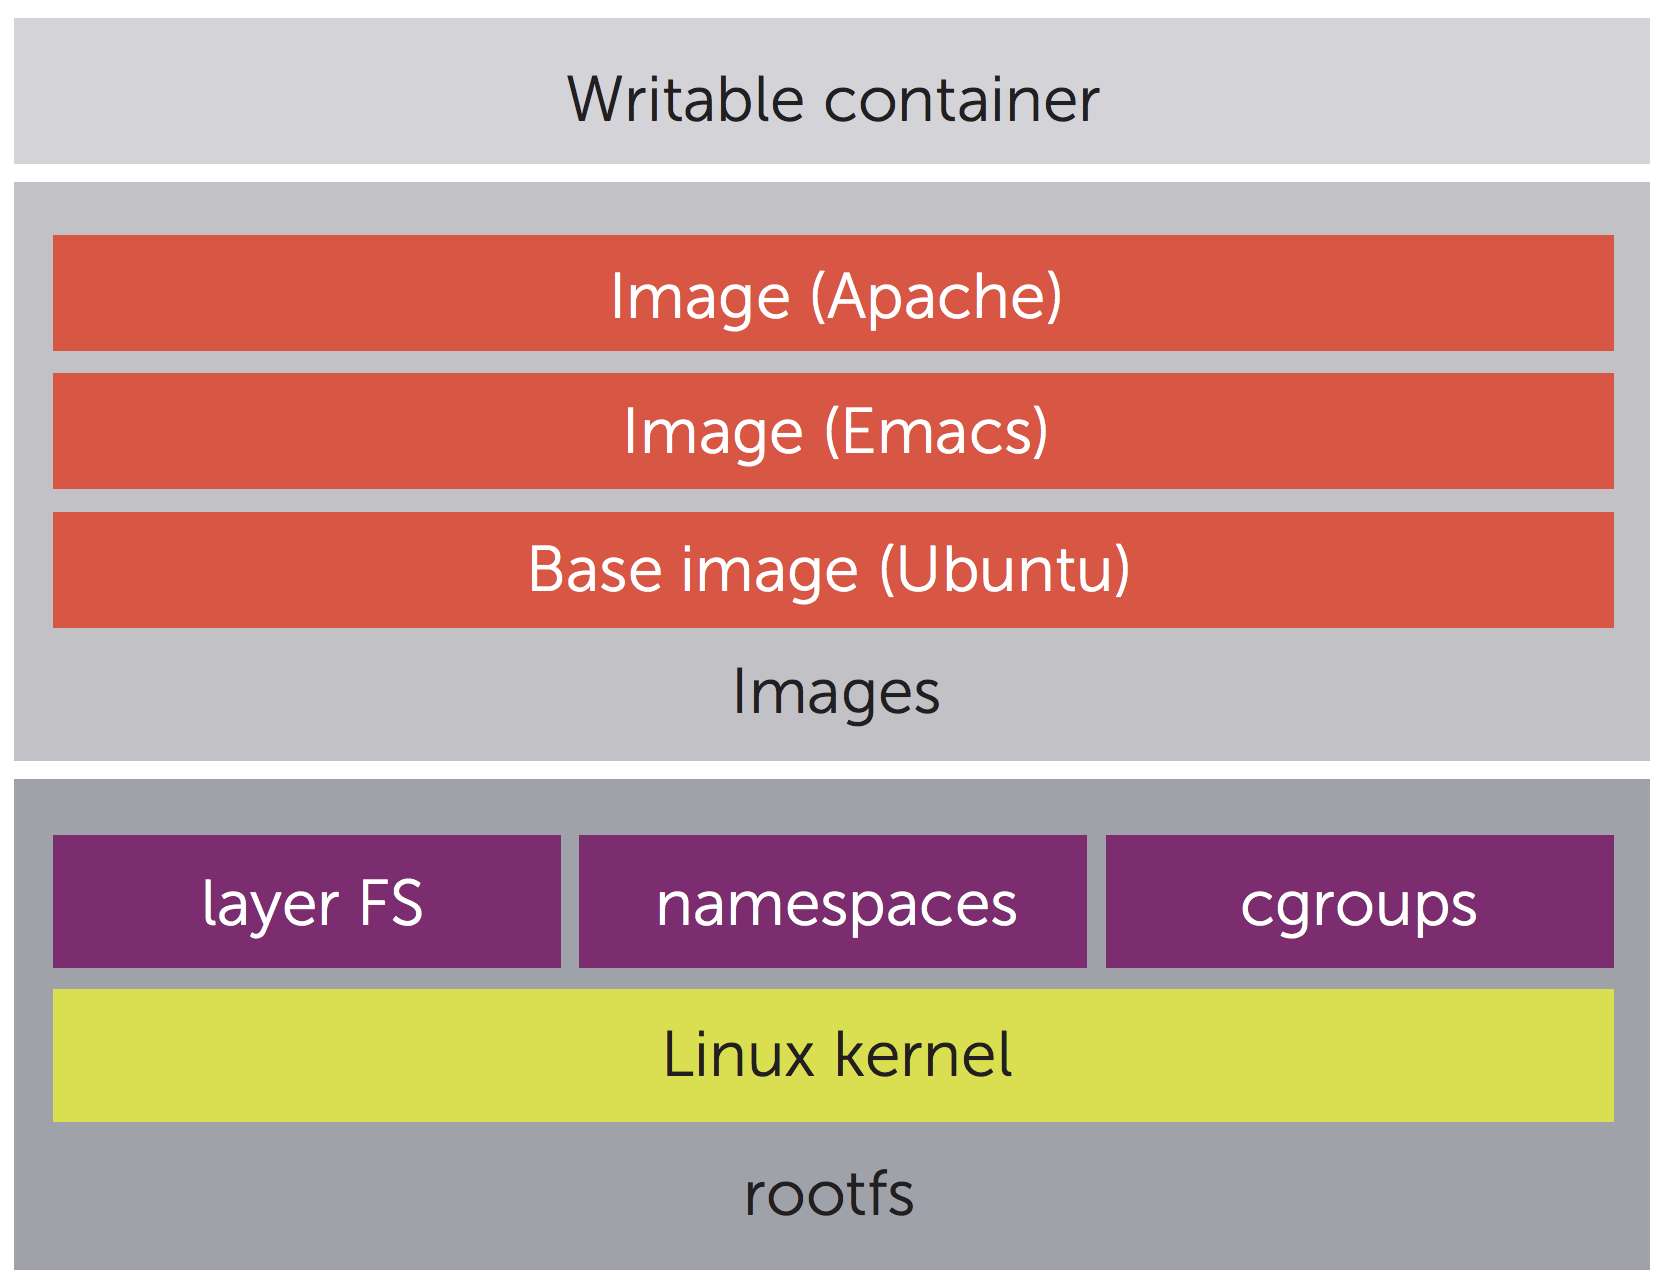
\includegraphics[width=0.5\textwidth]{chapter-background/docker-layers.png}
\end{figure}

\section{Container Orchestration}
Container technologies such as Docker offer advanced features to use containers in production. These solutions often offer deployment of applications limited to single machines. However, applications offered by  SaaS providers may include multiple different containers working together running on a cluster of nodes. Container orchestration (CO) systems allow deployment and management of containers at scale. Popular orchestration engines are Kubernetes, Docker Swarm and Mesos Marathon.
\subsection{Key capabilities of a container orchestration platform}
The task of a container orchestration (CO) platform is not limited to the initial deployment but the entire life-cycle of multiple containers. The goal of CO is to simplify cluster management while ensuring fault tolerance, availability, scalability and reliability. Allowing users to benefit from the complete potential of containers. In order to meet this goal, CO platform must at least offer the following key capabilities.~\cite{khan2017key}
\paragraph{Cluster state management and scheduling}
A cluster can be composed out of multiple virtualized or physical instances. Running containers on top of these instances and recover from failures requires a stable cluster. State management encapsulates various tasks such as flexible scheduling, re-partitioning of resources and data and propagating of dependent system changes.~\cite{khan2017key} 
\paragraph{High availability and fault tolerance}
A container orchestration platform must ensure high availability and fault tolerance in order to be useful for application developers. Most platforms therefor employ design principles of reliability engineering e.g., single point of failure elimination, failure detection or load balancing.~\cite{khan2017key}
\paragraph{Security}
Containers executing on top of the platform essentially form untrusted entities, with potentially malicious intentions, a high security standard is required. The standard should include: container images sanity check policies, access control for both containers and users, and techniques to minimize the container attack surface.~\cite{khan2017key}  
\paragraph{Simplified networking}
Containers must be able to communicate across nodes in  an efficient and secure manner. This requires the mapping of allocated host ports to containers. The overhead corresponding to this mapping intensifies at scale. The CO platform should thus provide a flexible, secure and scalable solution for networking.~\cite{khan2017key}
\paragraph{Service discovery}
The large number of services present in a cluster need to be able to communicate with each other. In traditional clusters services were handled as pets (i.e, having static names, IP addresses), however, in dynamic environments such as container orchestration platforms, they are regarded as cattle. The CO platform must provide mechanisms for addressing/labeling/grouping and service discovery.~\cite{khan2017key} 
\paragraph{Monitoring and governance}
The container orchestration platform needs to support traditional monitoring techniques such as logging, resource usage and network trace-routes. Monitoring must be possible at both the level of the underlying infrastructure and the containers themselves.~\cite{khan2017key}
\paragraph{Integrating for continuous integration and delivery}
Software development teams should be able to integrate the CO platform within their employed continuous integration and delivery (CI/CD) pipeline. The CO platform should contain mechanisms for rolling updates, rollbacks, etc.~\cite{khan2017key}


\subsection{Kubernetes}
Kubernetes~\cite{kubernetes}, commonly referred to as K8,  is one of the most popular and adopted orchestration systems. It is an open-source project led by Google. Kubernetes is Google's solution for the growing demand of container deployments by external developers in its public business cloud and is based upon its predecessors  Borg~\cite{verma2015large} and Omega~\cite{schwarzkopf2013omega} that have been used to schedule the internal Google workload. Its main design goal is formulated as:\textit{ "to make it easy to deploy and manage complex distributed systems, while still benefiting from the improved utilization that containers enable~\cite{Burns:2016:BOK:2930840.2890784}"}.  \\\\
\noindent To achieve the above stated goal Kubernetes introduces a number of concepts for both containers and cluster resources. It implements the infrastructure as code model  by provides an abstraction layer on top of the physical infrastructure~\cite{hermanns2015current}. It allows to setup and manage container infrastructure by the configuration of these introduced concepts via a REST API or declarative YAML configuration files. Below the most relevant concepts are introduced.
\subsubsection{Kubernetes concepts}
\textbf{Pods.}  A pod is the smallest unit of deployment within Kubernetes. It is a group of one or more containers that logically belong together.   A pod and thus its containers run on the same node. They share the same network, storage and context (Linux namespaces, cgroups). A pod gets assigned a unique IP address. Pods are not self-healing meaning when an error occurs within the pod or during scheduling. It will be deleted. Due to this short life cycle using a single pod resource and its assigned IP address for applications is impractical. Kubernetes handles this by employing controllers and services.~\cite{pods}\\\\
\textbf{Deployments.}  A Deployment controller manages a pod or a ReplicaSet of pods. A ReplicaSet allows pods to be replicated across multiple nodes. A Deployment object is used to specify the desired state of pods (e.g. number of replica's). A deployment, in addition, allows for declarative updates. These updates can be used to change the number of container replicas of a ReplicaSet or to update a specific container image within the pod.  The Deployment controller changes the actual state to the desired state described by the update.~\cite{deployments}
\\\\
\textbf{Services.}  Services offer a solution for the short life cycle of pods (and their IP addresses). Services within Kubernetes offer a manner to expose a ReplicaSet of Pods via a unique name, stable IP address, network policy and ports. To determine which set of pods is targeted by a service, Kubernetes employs a Label selector. Labels are the core grouping primitive of Kubernetes and unlike names and UIDs do not offer uniqueness.\\  A Service can be exposed outside the cluster by using an external load balancer or by specifying a NodePort. When using a Nodeport each node within the cluster will expose the port and forward request into the service.~\cite{services}
\\\\
\textbf{Namespaces.}  Namespaces allow to partition resources of a physical cluster among multiple user organizations. Each namespace gets a share of the resources of the cluster, via resource quotas. Resource quotas are supported for CPU, memory and persistent volumes.~\cite{namespaces-k8}
\\\\
\textbf{Resource limits.}  Kubernetes allows the allocation of compute resources of both containers and Namespaces by the means of resource limits. These limits can be soft (limit) and hard (request) limits. A Request specifies the quantity of resource that is guaranteed to the container. A limit specifies the maximum quantity allocated to the container. When the requested resource quantities of a container are less than its limit, the container may be allocated additional resources if there are unallocated resources available.  The current supported compute resources are CPU, memory and storage within the root partition of the local node. Within a Pod it is possible to specify both request and limit for each container. When request and limits are specified, the scheduler will use them for both scheduling and eviction (when node capacity is reached) decisions.~\cite{kubresources}
\subsubsection{Kubernetes architecture}
The basic architecture of Kubernetes is illustrated in Figure~\ref{fig:kubarch}. A client-server architecture is employed in which master and node setups are deployed on different machines. Below the different components that build up the architecture are briefly explained. 
\paragraph{API Server.} The API server is responsible for the configuration and validation of API objects (pods, deployments, services,...). It offers communication on cluster state via a REST interface for both components and administrators.~\cite{kubernetes-api-server}
\paragraph{Controller manager.} The controller manager is responsible for managing several core control loops part of Kubernetes. A control loop uses the API server to observe the shared state of the cluster and attempts to move to the desired state via configuration changes.~\cite{kubernetes-controller-manager}
\paragraph{Scheduler.} The task of assigning pods to nodes is the responsibility of the scheduler component.  The scheduler attempts to do a reasonable placement based on resource and quality of service requirements (e.g., not place a pod on a node with insufficient resources). It is  possible for users to control the placement of pods via NodeSelector tags or affinity and anti-affinity constraints in the configuration file.~\cite{kubernetes-pods-to-nodes,kubernetes-scheduler}
\\\\In addition it is possible to assign Quality of Service (QoS) classes to pods. These are used by Kubernetes in the decision process about scheduling and eviction of pods. Currently, Kubernetes supports three types of classes: guaranteed, burstable and best-effort. In decreasing order of priority (i.e., most likely to be killed in the case of resource shortages). The QoS classes are assigned to pods based on the presence of request and limit specifications of resources in their configuration files.~\cite{kubernetes-qos}


\paragraph{Kubelet.} The kubelet component is an agent running on each node. It is responsible for running and maintaining pods on its residing node. The set of maintained pods is described in the form of PodSpecs (mainly received via the API-server).~\cite{kubernetes-kubelet}
\paragraph{Kube-proxy.} The kube-proxy daemon provides a simple network proxy for the services on each node. It enables forwarding of requests to the correct containers and can provide primitive load balancing.~\cite{kubernetes-kubeproxy}
\begin{figure}[H]
\caption{Kubernetes architecture}
\centering
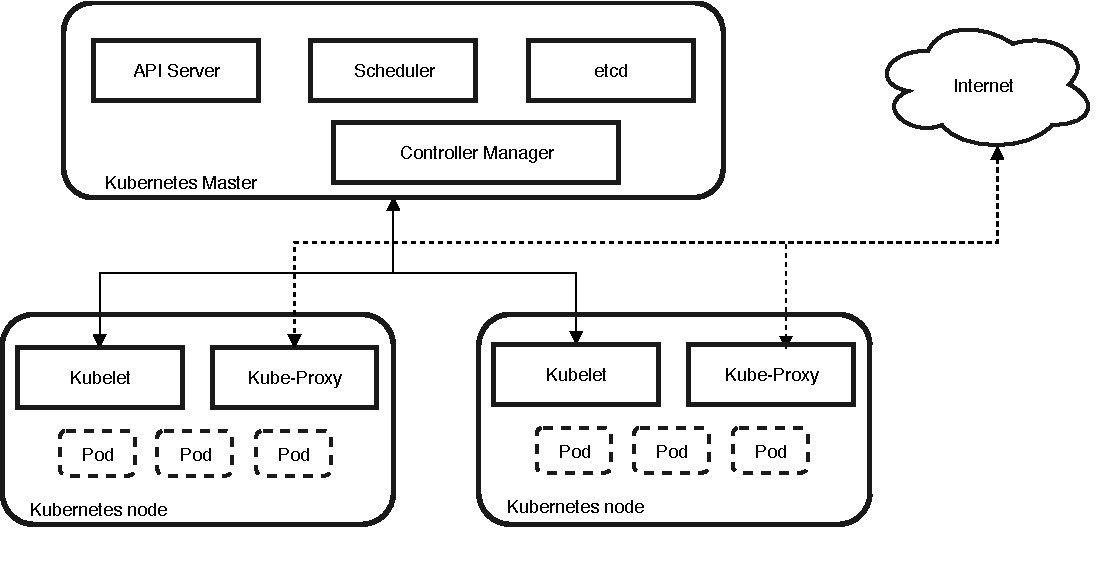
\includegraphics[width=0.8\textwidth]{chapter-background/kubernetes-architecture-diagram.pdf}
\label{fig:kubarch}
\end{figure}
 
 
 
 
 
 
 
 
 
 \section{Performance evaluation}
As discussed in previous sections, SaaS providers employ multi-tenancy to improve  cost efficiency and offer several performance guarantees to their customers in the form of SLOs. An unavoidable consequence of multi-tenancy is the need to support a growing number of users in a single system. Providers need to have a clear insight into the \textit{scalability} of their systems. However, scalability is a difficult thing to define, let alone quantify. Citing the words of  Dr. Neil J. Gunther:  \textit{"if you can't quantify it, you can't guarantee it"}.~\cite{perfdynamics}

\subsection{The Universal Scalability Law}
\label{section-USL}
Dr. Neil J. Gunther provides a formal definition of scalability: \textit{"scalability can be defined as a mathematical function, a relationship between independent and dependent variables (input and output)"~\cite{perfdynamics}}. The Universal Scalability Law (USL) by Dr. Neil J. Gunther is presented in Equation~\ref{USL}. It computes the relative capacity $C(N)$ at a load of $N$ users. Relative capacity is the normalized throughput.
\begin{equation}
\label{USL}
C(N) = \frac{\gamma~N}{1 + \alpha~(N-1) + \beta~N~(N-1)}
\end{equation}

The Universal Scalability Law incorporates factors that contribute to the sublinearly scalability of most systems. Namely, \textbf{concurrency} ($\gamma$), \textbf{contention} ($\alpha$) and \textbf{coherency} ($\beta$) as explained below. Their impact is visualized in Figure~\ref{fig:usl-impact}.

\begin{itemize}
    \item \textbf{Concurrency}($\gamma$): $\gamma$ defines the slope if the system was linearly scaling i.e., $C(N) = \gamma N$. It has been referred to as the \textit{coefficient of performance} by~\cite{schwarz2015practical}.
    \item \textbf{Contention} ($ \alpha $) : When scaling most systems parallelism while be limited at some point by contention (i.e., waiting or queuing for shared resources). The maximum speedup by parallelism is limited by the serialized portion ($\alpha$) of the work~\cite{schwarz2015practical}. 
    \item \textbf{Coherency} ($\beta$): created by crosstalk between components. Because crosstalk is possible between each pair of components in the system, the penalty grows quadratic $N(N-1)$.~\cite{schwarz2015practical}
    
\end{itemize}

\begin{figure}
    \centering
    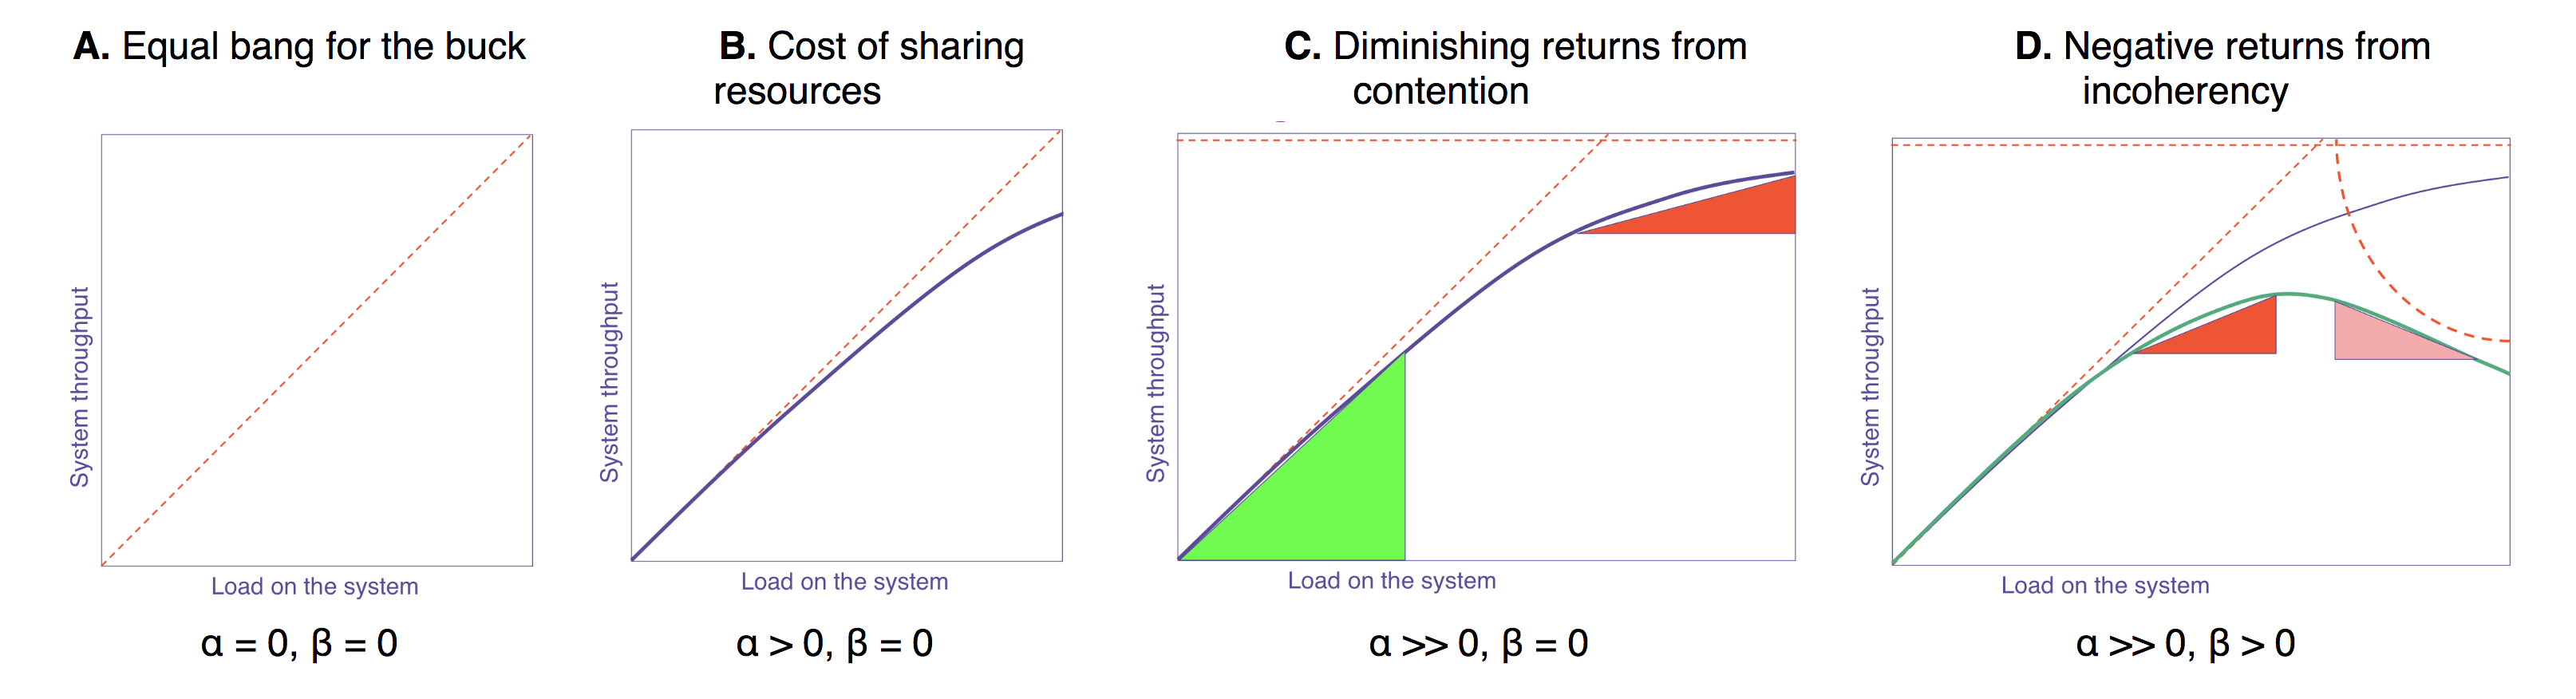
\includegraphics[width=1.1\textwidth]{chapter-evaluation/usl-impact}
    \caption{The impact of different USL coefficients on scalability.~\cite{perfdynamics}}
    \label{fig:usl-impact}
\end{figure}

\subsubsection{USL in practice}
USL can provide insights into a system's scalability pains via  values of the concurrency, contention and coherency coefficients. These can be obtained by collecting a dataset of measurements of the system, system load $N$ and corresponding throughput, and using a statistical technique such as nonlinear least square regression which fits the USL to the dataset.~\cite{schwarz2015practical,heyman2014scalability}

\subsection{Little's law}
\label{sec:little}
The Universal Law of Scalability serves as an alternative for the often less intuitive queuing models frequently used for modeling scalability. It omits the need to know the service time for every queue in the performance model in order to predict the response time or latency~\cite{perfdynamics}. Nevertheless, queuing theorem and its lemmas such as Little's Law can provide useful insights into performance modeling.\\\\
John D.C Little's Law~\cite{little2008little} states the following for stable systems: 
\begin{displayquote}
\textit{"The average number of items in a queuing system equals the average rate at which items arrive multiplied by the average time that an item spends in the system.\cite{little2008little}"}
\end{displayquote}
\begin{equation}
\label{littleslaw}
L = \lambda~W
\end{equation}
\begin{equation}
\label{llsys}
N = X~Rt
\end{equation}
Equation~\ref{littleslaw} shows Little's law, below its terms and its applicability to web services (Equation~\ref{llsys}) are explained:
\begin{itemize}
    \item \textbf{$L$}:  Average number of items in the system. For a web service this is represented by the average number of concurrent users in the system $N$.
    \item \textbf{$\lambda$}: Long-term average arrival rate of items in the system per time unit. Little's law assumes a stable system for which the arrival rate and exit rate are identical. In a web service this is represented by the throughput $X$.
    \item \textbf{$W$}: Average waiting time of an item in the system, queuing time and service time combined. This is represented by the response time $Rt$ or latency of a request in a web service. When dealing with a system involving think time (e.g., after the response from a web service, a user needs time to think about his/her next request), $(Rt + Zt)$ is used. 
\end{itemize}

\subsubsection{Workload generator validation}
Developers employ software tools (JMeter~\cite{jmeter}, Locust~\cite{locust}, etc.)  to simulate a workload and test the performance of a system. A workload is a set of actions that represent the behavior of a client in the system. It is part of the test plan stating the number of concurrent users $N$ executing the workload for a specified period of time.\\\\
The results of a performance test are typically expressed in throughput $X$ and response time $Rt$. Using Little's law it is possible to validate these results. For example, a test plan of 1000 concurrent users $N$ results in a throughput of 50 requests per second and an average response time of 15 seconds. Following Little's law, a concurrence of only 750 users was reached, instead of the specified 1000. Little's law can thus be used to check if a workload generator works as specified.\\\\
Alternatively, if the average throughput and response time for a production system are known, Little's law can be used to correctly draw up a test plan.

\subsubsection{Response time or latency?}
Performance can either be measured in throughput or latency, both are correct but offer a different point of view. System performance is typically expressed in throughput: "The system can handle a million operations per second". However, users care more about their personal experience with a system which is influenced by the average latency of their request.~\cite{schwarz2015practical} \\\\
Figure~\ref{fig:ls_vs_tp} shows the relation between the average latency and throughput of a database under increasing load $N$. In this case, latency is kept stable by increasing the throughput with the increasing load up to a certain point.  A bottleneck caps the throughput of the systems and by Little's law for an increasing load and constant throughput, the latency must increase.~\cite{latvsthrough} \\\\
However in other systems, as discussed in Section~\ref{section-USL}, an increasing load might induce a diminishing result on the system's throughput. Following Little's law a decreasing throughput results in a higher latency under the same load. \\\\
Thus, for stable systems by Little's law,  the USL can be reformulated in terms of latency instead of throughput. Equation~\ref{USL-2} shows this reformulation.~\cite{schwarz2015practical}
\begin{equation}
\label{USL-2}
Latency(N) = \frac{1 + \alpha~(N-1) + \beta~N~(N-1)}{\gamma}
\end{equation}


\begin{figure}[H]
    \centering
    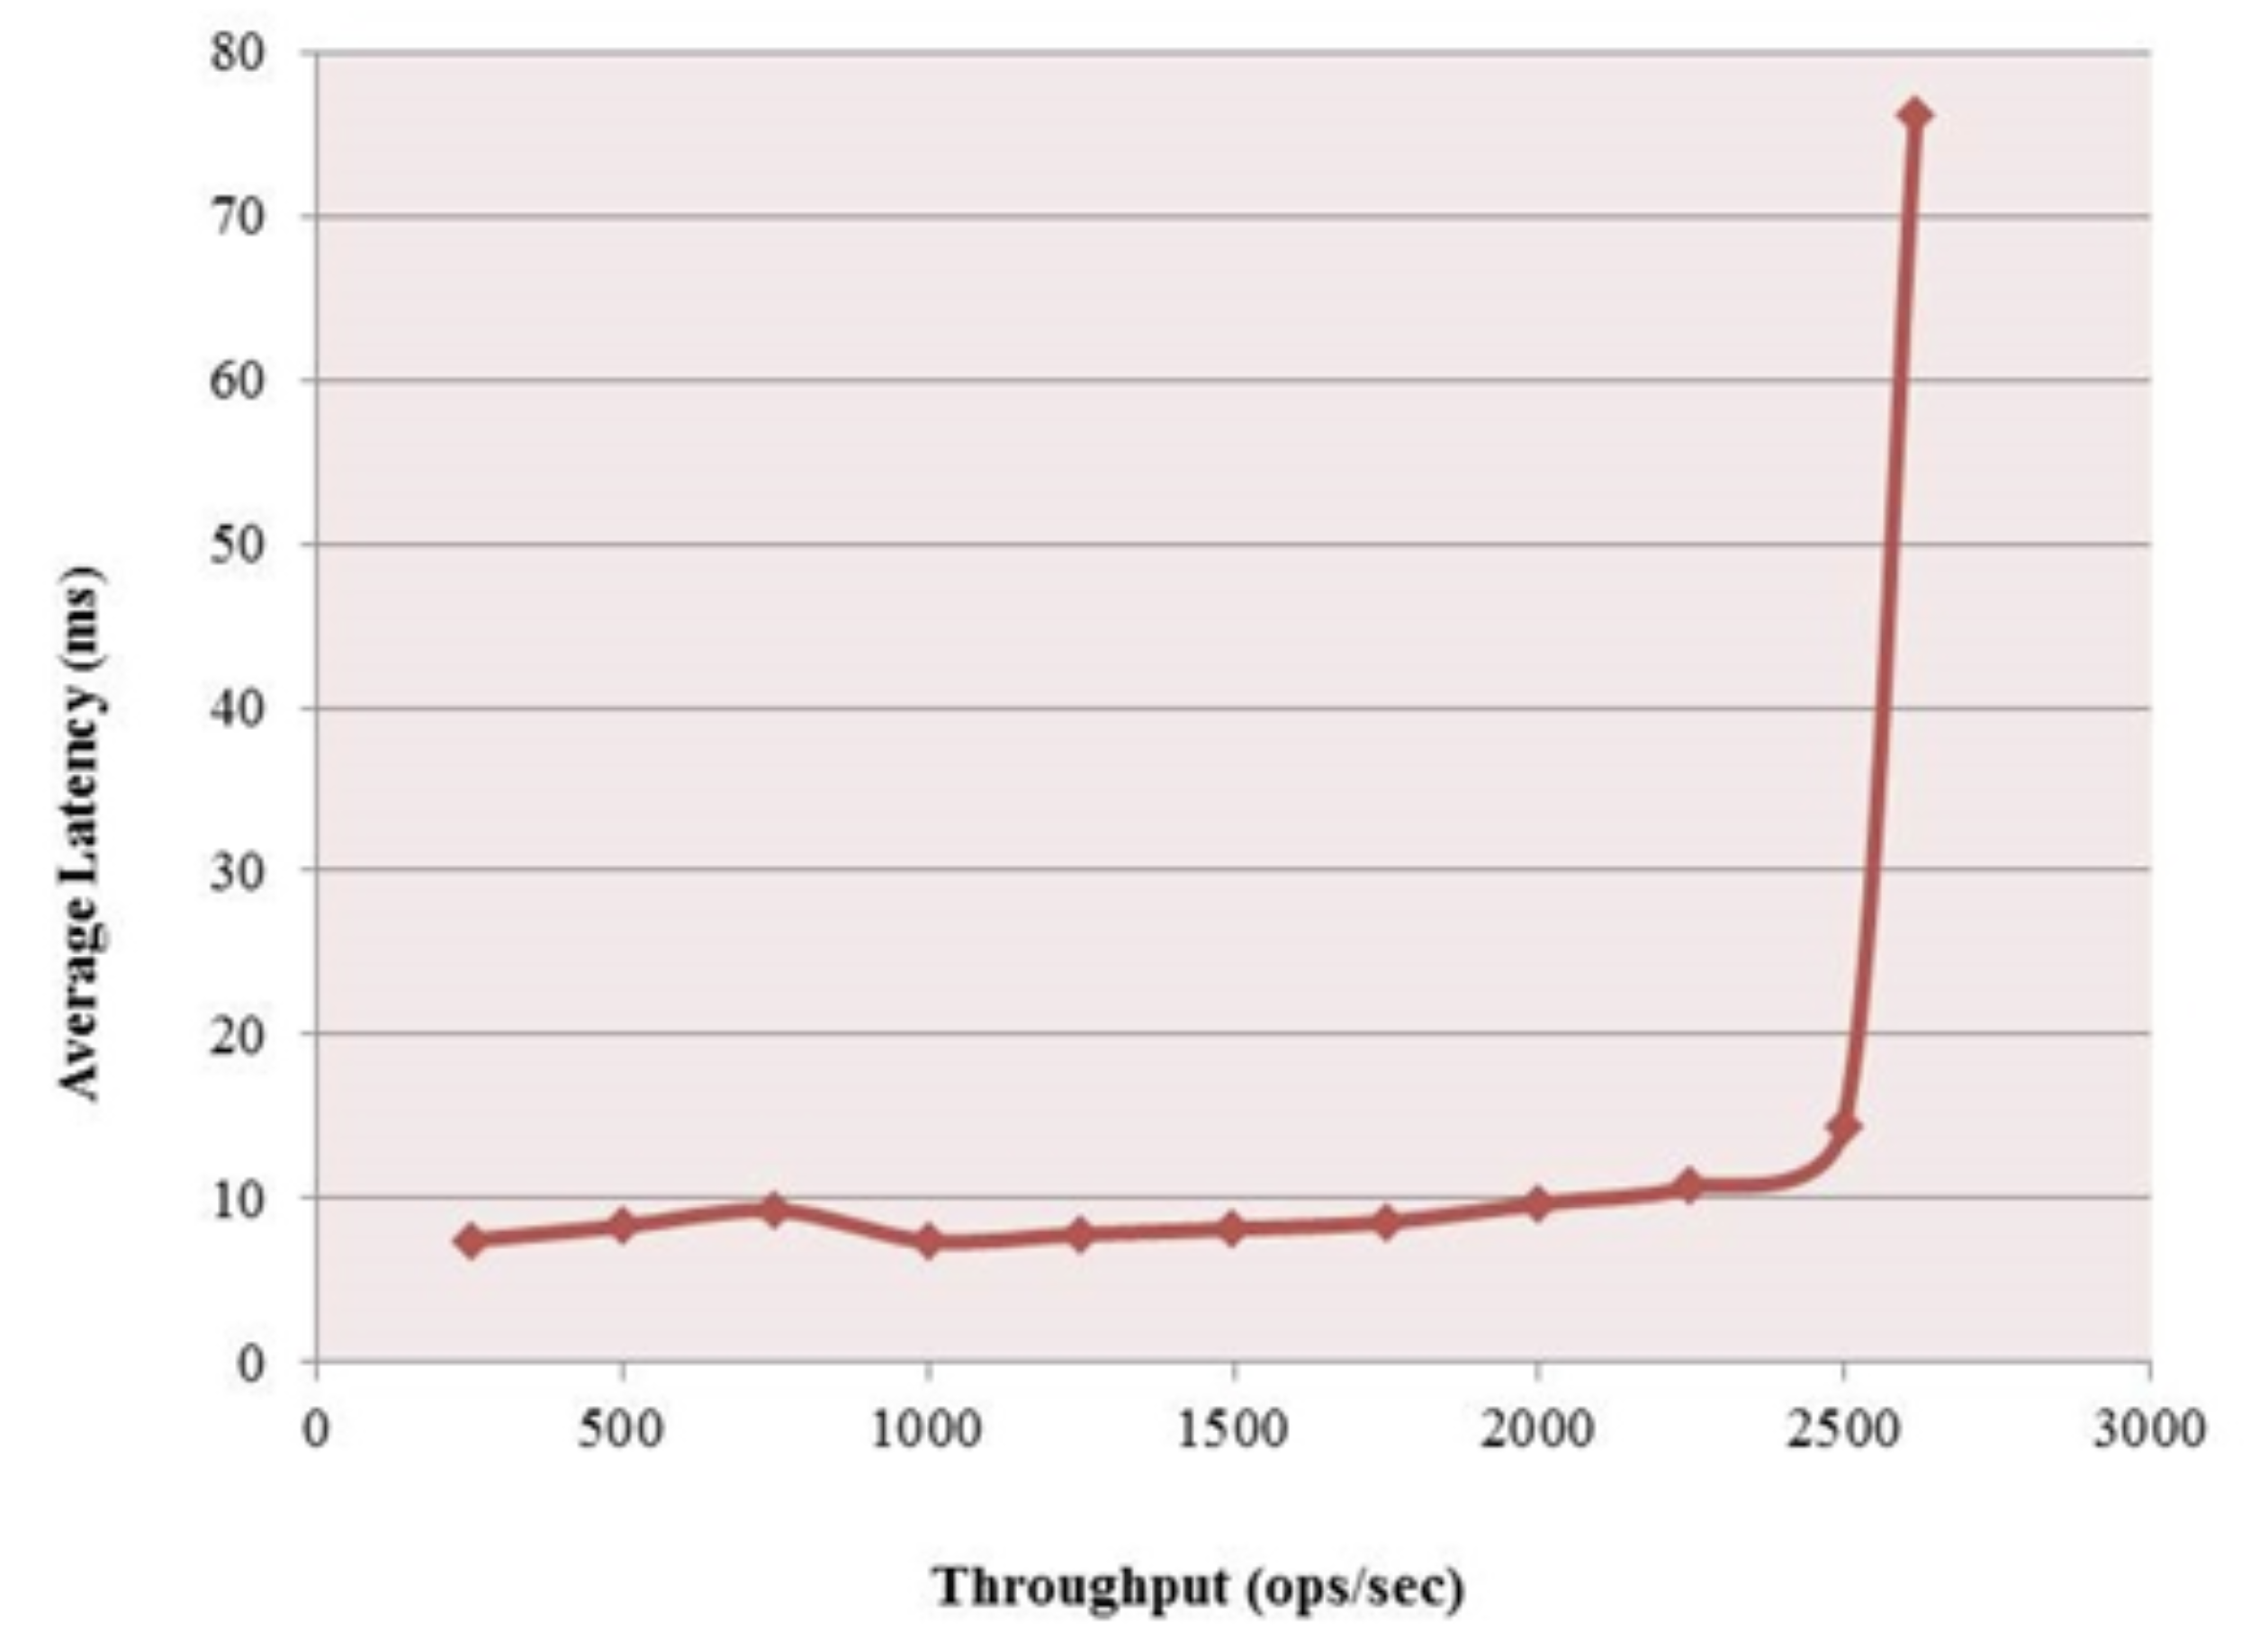
\includegraphics[width=0.8\textwidth]{chapter-evaluation/ls_vs_th}
    \caption{Relation average latency vs. throughput for database benchmark with increasing load.~\cite{latvsthrough}}
    \label{fig:ls_vs_tp}
\end{figure}
\chapter{Background}
\label{ch:background}
This chapter discusses relevant background material for the thesis. The concepts, explored in this chapter, further clarify the relevance of the thesis and serve as building blocks for the remaining chapters. Starting from the adoption of the cloud computing paradigm, the chapter elaborates on how concepts such as multi-tenancy and virtualization via containerization push the limits of efficient resource utilization. Next, an in-depth overview of the open-source container orchestration platform Kubernetes is provided. Lastly, insights are provided into the universal scalability law and the applicability of Little's law for performance testing.
\section{Cloud computing}
Companies try to minimize the total cost of ownership by moving to cloud computing or utility computing. The cloud computing paradigm enables on-demand access to a shared pool of configurable compute resources (software applications, system software and hardware infrastructure)~\cite{WalravenStefan2015PPmf}. A service provider can provision the required resources from the cloud with minimal effort.  Within this paradigm, services are offered in real time over the internet in three different models~\cite{MellPeter2010TNDo,rimal2009taxonomy}. 
\begin{itemize}
\item \textit{Infrastructure as a Service (IaaS)} in which access is offered to virtual machines, network, data storage and other fundamental computing resources. The customer is able to deploy arbitrary software using these resources.\\\\
Examples: Digital Ocean, Microsoft Azure and Amazon Elastic Compute Cloud (EC2).
\item \textit{Platform as a service (PaaS)} offers customers a platform enabling easy and efficient deployment of applications (at scale) while abstracting the complexity of managing the underlying infrastructure. PaaS allows customers to solely focus on the development of their application.\\\\
Examples: Google app engine, Microsoft Azure and Heroku.
\item \textit{Software as a service (SaaS) } allows customers to make use of a specific application developed by a SaaS provider. Compared to the traditional use of software, the management and deployment is the task of the SaaS provider. In this strategy, common resources and a single instance of both the application and underlying database are used to support multiple customers simultaneously. \\\\
Examples: Google apps and Salesforce.
\end{itemize}

\section{Multi-tenancy}
\label{multi-tenancy}
The software as a service (SaaS) model offers applications to customers as an on-demand service. Providers of these applications try to leverage economies of scale by employing a multi-tenancy architectural design principle. The goal of multi-tenancy is to minimize the total cost of ownership for the provider by maximizing the sharing of resources among multiple customers organizations, referred to as tenants.~\cite{Walraven2015b} 
\subsection{Service Level Agreements}
By moving their core business functions to an entrusted cloud provider, cloud customers give up control of the underlying compute resources. It is vital for these tenants to obtain certain guarantees on the service delivered by the provider. 
A Service Level Agreement (SLA) is a formal contract between the SaaS provider and the tenant specifying both properties of the provided service and the expected behavior of the tenant. An SLA typically also contains a set of Service Level Objectives (SLOs). An SLO is a measurable characteristic of the service. An SLO is typically related to performance constraints (latency, throughput and deadlines) or availability (uptime percentage) of the service. Within the specification of an SLA a trade-off must often be made between expressiveness and usability. The SLA must cover all the expectations of a customer while remaining simple to weight, verify, evaluated and enforce~\cite{dillon2010cloud}.  Some typical examples of SLOs are shown below: 
\begin{itemize}
\item The application has a monthly uptime percentage of 99.95\%.
\item If the arrival rate of the tenant workload < X requests/s then a throughput T is guaranteed.
\end{itemize}
\subsection{Challenges}
While the goal of multi-tenancy is promising, sharing a cluster of dynamically provisioned nodes between multiple tenants imposes a number of challenges and requirements~\cite{TruyenEddy2016Taca}. 
\begin{itemize}
\item Performance isolation: the activities of one tenant should not be able to influence the service level delivered to other tenants. This requirement should be achieved during normal system load and when an aggressive tenant violates the terms of the SLA. 
\item QoS differentiation: the performance guarantees specified by an SLA can be individually customized for each tenant. A SaaS provider should be able to offer different subscriptions.
\item Flexible resource allocation for improved server consolidation: a SaaS provider employs a multi-tenant architecture to achieve a lower operational cost. This is partially achieved by planning the required node capacity based on the actual resource usage of tenants instead of the theoretical required capacity.  This can be further aided by the use of request schedulers allowing to distinguish between normal, passive and aggressive tenants. 
\end{itemize}
\subsection{Strategies}
To achieve multi-tenancy different strategies, each offering different trade-offs concerning operational costs and upfront application engineering costs, can be employed by the SaaS-provider~\cite{WalravenS.2011Amlf}. The strategies are illustrated in Figure~\ref{muti-tenant-strategies}.
\begin{itemize}
\item Multi-tenancy can be achieved at the level of the \textit{operating system}. In this strategy, a virtualization technology can be used to partition compute resources among multiple virtual machines. Each tenant is assigned an application instance running on a dedicated virtual machine. This approach offers both a higher level of performance isolation and lower upfront engineering costs but suffers from an inefficient utilization of resources.
\item In \textit{middleware-level multi-tenancy} a middleware platform is used to enable sharing compute resources between multiple tenants at the level of the operating system. An application instance is deployed on top of the middleware platform for each tenant. By not replicating the operating system for each tenant a higher level of cost efficiency can be achieved but an increased complexity in managing resources and  performance isolation is introduced. By tackling these problems at the level of the middleware a part of the engineering complexity is shifted to this level.
\item The most efficient resource utilization can be achieved by sharing application instances between multiple tenants. In \textit{Application-level} multi-tenancy achieving performance isolation is done by the application itself thereby increasing the engineering complexity and costs.
\end{itemize}


\begin{figure}[H]

\caption{Different strategies to achieve multi-tenancy~\cite{WalravenS.2011Amlf}.\label{muti-tenant-strategies} }
\centering
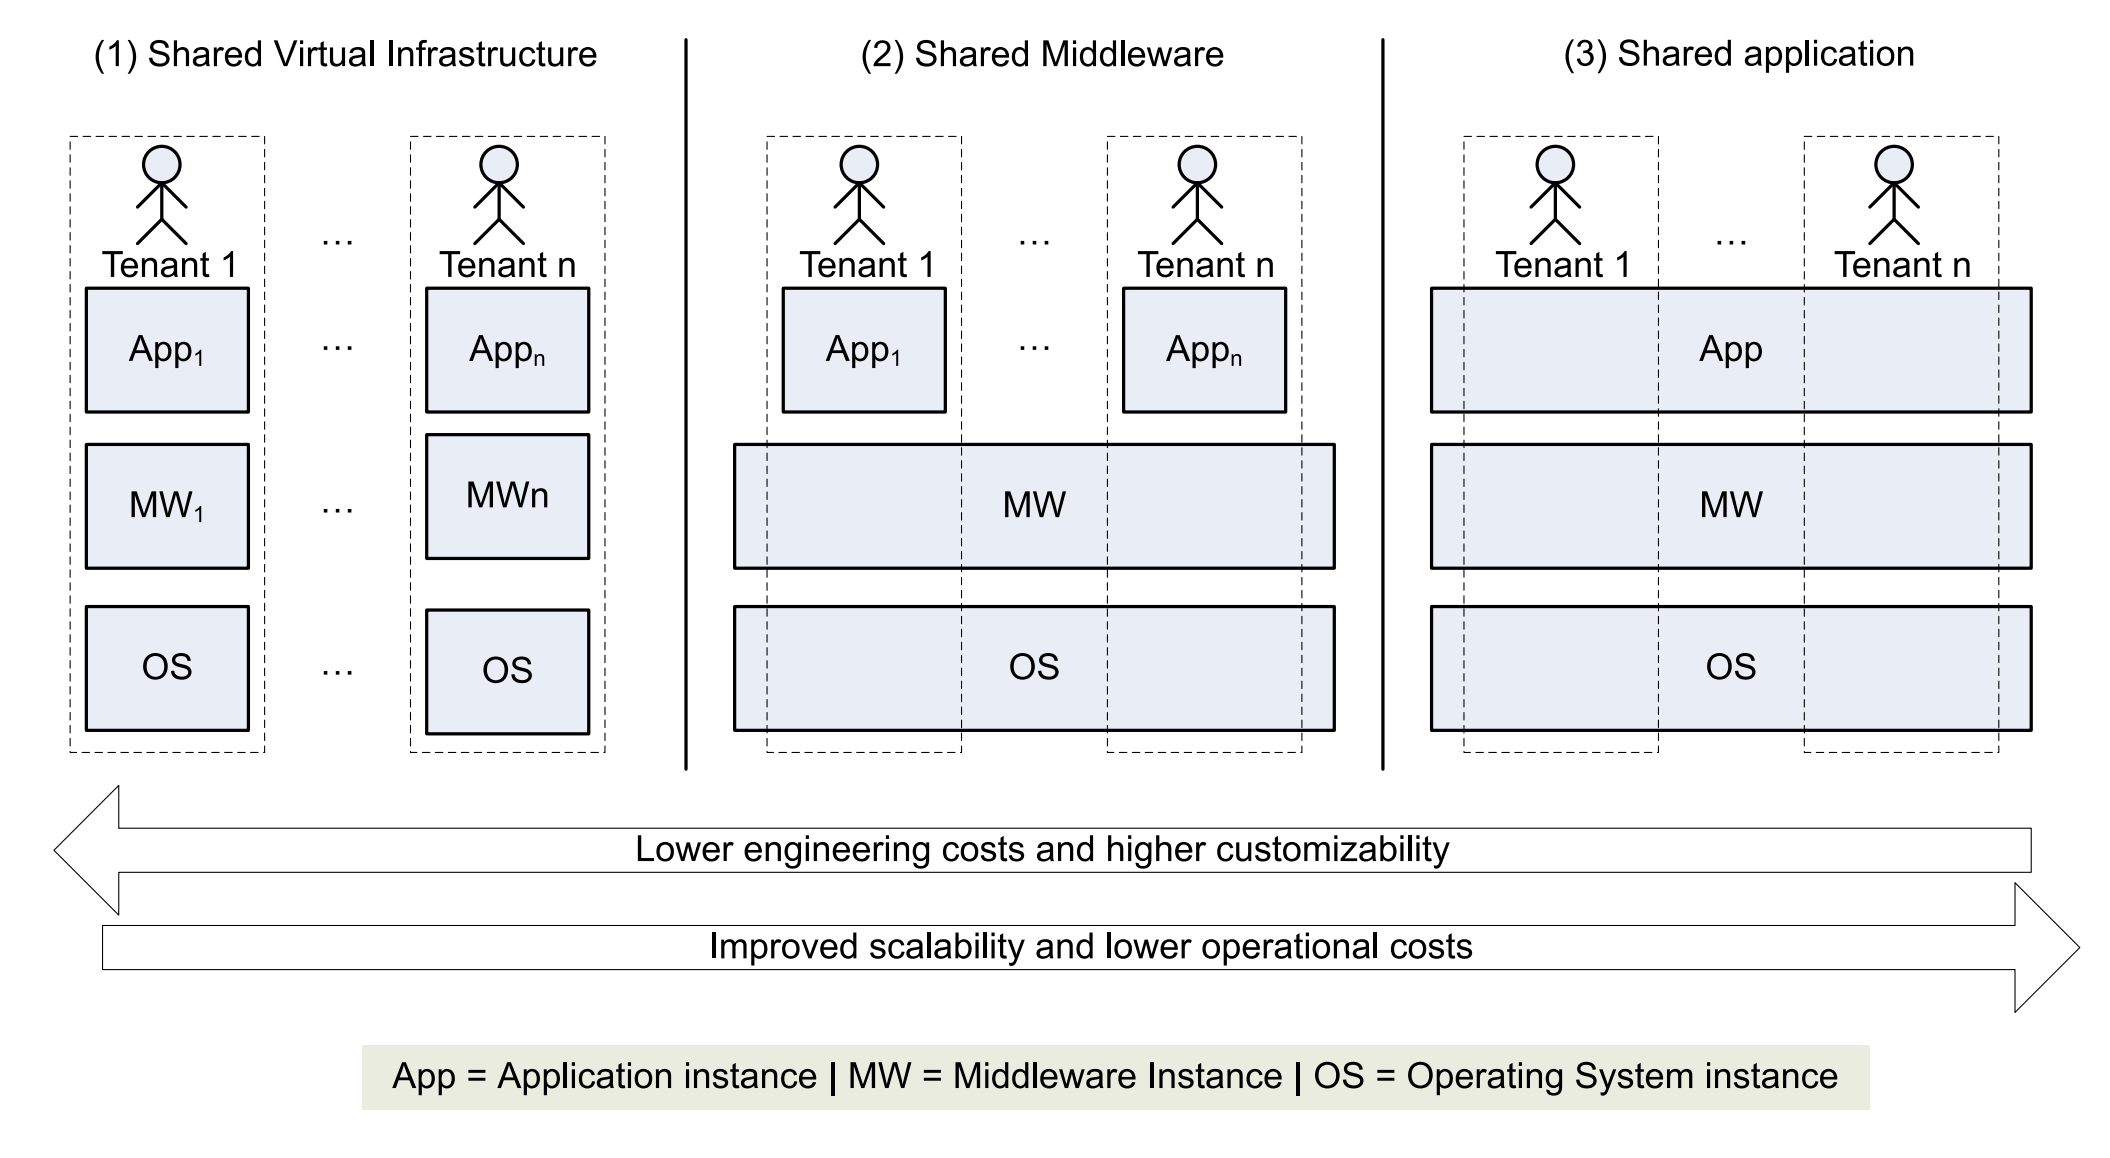
\includegraphics[width=0.65\textwidth]{chapter-background/muti-tenant-strategies.png}
\end{figure}


\section{Containerization}
Cloud providers rely on virtualization technology for the achievement of large-scale resource scaling. For more than a decade, virtual machines (VMs) have been the backbone of a provider's infrastructure offering hardware independence, availability, isolation and security~\cite{xavier2013performance}. More recently, containers a more lightweight virtualization technology have made advances in their multi-tenant capabilities and have seen an increase in adoption by providers~\cite{pahl2015containerization}. Both are discussed in this section.
\subsection{Virtualization technology}
In cloud environments, virtualization technology is used for flexible and dynamic allocation of physical resources to virtualized applications and to achieve multi-tenancy by sharing a physical server among multiple applications. In data centers virtualization is commonly used at the \textit{hardware level} and \textit{operating system level} to deploy and manage virtual machines and applications at scale~\cite{SharmaPrateek2016CaVM}. \\\\
Hardware level virtualization uses a hypervisor on a server to create virtual machines. Each virtual machine provides an abstraction of a physical machine and runs an independent operating system with applications. The hypervisor is responsible for resource allocation and performance isolation.\\\\
Operating system level virtualization allows resources to be shared at the level of the OS. Virtual machines running at the OS level are referred to as containers. Isolation, abstraction and resource allocation of containers is performed by the OS kernel of the host OS. By sharing the OS kernel among multiple containers, containers are regarded as a more lightweight virtualization technology. Containers only contain the application and its dependencies.\\\\
Linux containers (LXC)~\cite{lxc} employ different mechanisms of the Linux kernel to achieve resource isolation, namely control groups and namespaces.
\begin{itemize}
    \item \textbf{Cgroups}~\cite{cgroups} allow for fine-grained control of the allocation of system resources (CPU time, system memory, network bandwidth) among processes and process groups. For example, it is possible to limit or prioritize memory, CPU or I/O usage of different containers. 
    \item \textbf{Namespaces}~\cite{namespaces} allow for isolation of kernel resources among processes. A namespace makes a resource appear to be private and isolated for the container. The Linux kernel provides the following namespaces:  process ids, inter-process communication (IPC) mechanisms, network stack and mount points.
\end{itemize}
Linux containers (LXC) offers a lightweight implementation which performs at native speed and provides good isolation. However, while sharing a kernel between containers minimizes overhead, there are limitations in terms of the security environment.~\cite{dua2014virtualization}
\\\\
\noindent By offering virtualization at different levels, containers and VMs offer different trade-offs concerning performance isolation and performance. Research~\cite{SharmaPrateek2016CaVM} concludes that while containers offer closer to bare metal performance compared to VM, they offer worse performance isolation in multi-tenant environments. In addition, containers offer soft resource limits compared to the hard resource limits of virtual machines which allow for better server consolidation in over-commitment scenarios.  
\begin{figure}[h]
\caption{Container vs virtual machine.~\cite{container-vs-vms}}
\centering
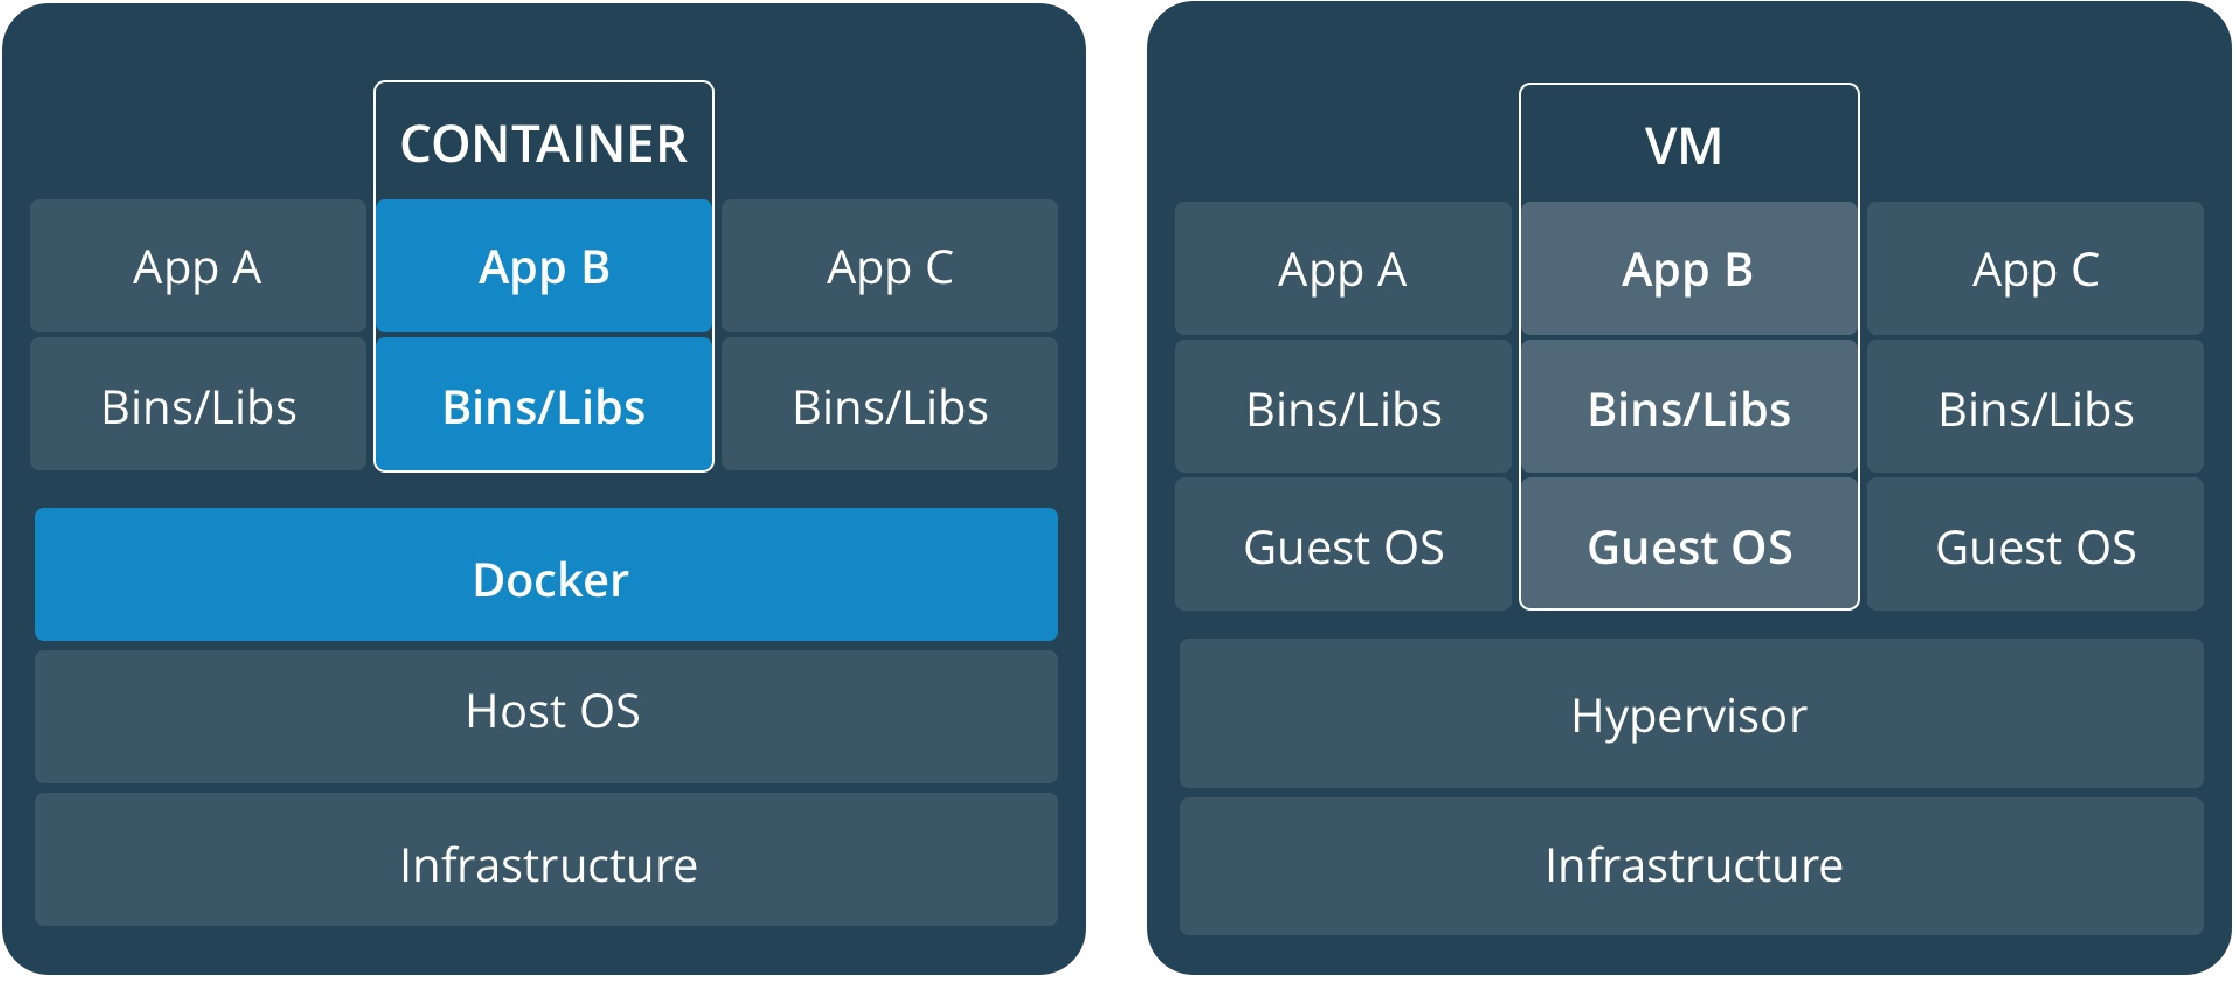
\includegraphics[width=0.8\textwidth]{chapter-background/containervsvm.pdf}
\end{figure}
\subsubsection{Docker}
Recently, thanks to Docker~\cite{dockersite}, containers have gained popularity and have been adopted into the software development process. However, Docker is not a new container technology, at its core it employs the kernel-level mechanisms of Linux containers (LXC), for which it defines a unified API~\cite{merkel2014docker}. In addition, the open-source Docker project offers a commandline-interface and daemon that offers easy packaging of applications in containers and the deployment of these containers.\\\\
To achieve this Docker introduces the concept of images. A container is represented by a lightweight image. A container image is a lightweight, executable package containing an application and its dependencies (runtime, libraries, environment variables, and config files). Virtual machines (VMs) can be seen as full, monolithic images. In particular,  Docker image consists of file-system layers stacked upon each other, as illustrated in Figure~\ref{docker-layers}. Only the top layer, the container itself, is writable, therefore it is state-full and executable. A container is thus composed out of layers of individual images built on top of a base image, allowing for easy extensibility.~\cite{pahl2015containerization} \\\\
A Docker image is specified by and build from a DockerFile. Images can be made easily accessible through Docker registries such as Dockerhub.\\
These images allow for easy and fast deployment of Docker containers across different operating systems and cloud provider stacks. Resulting in a game-changing technology for DevOps, system administrators and developers.
\begin{figure}[H]
\caption{Architecture of a container image. Images can be stacked upon each other using the cgroups and namespace extensions of a Linux kernel. The top container image is writable.~\cite{pahl2015containerization} \label{docker-layers}}
\centering
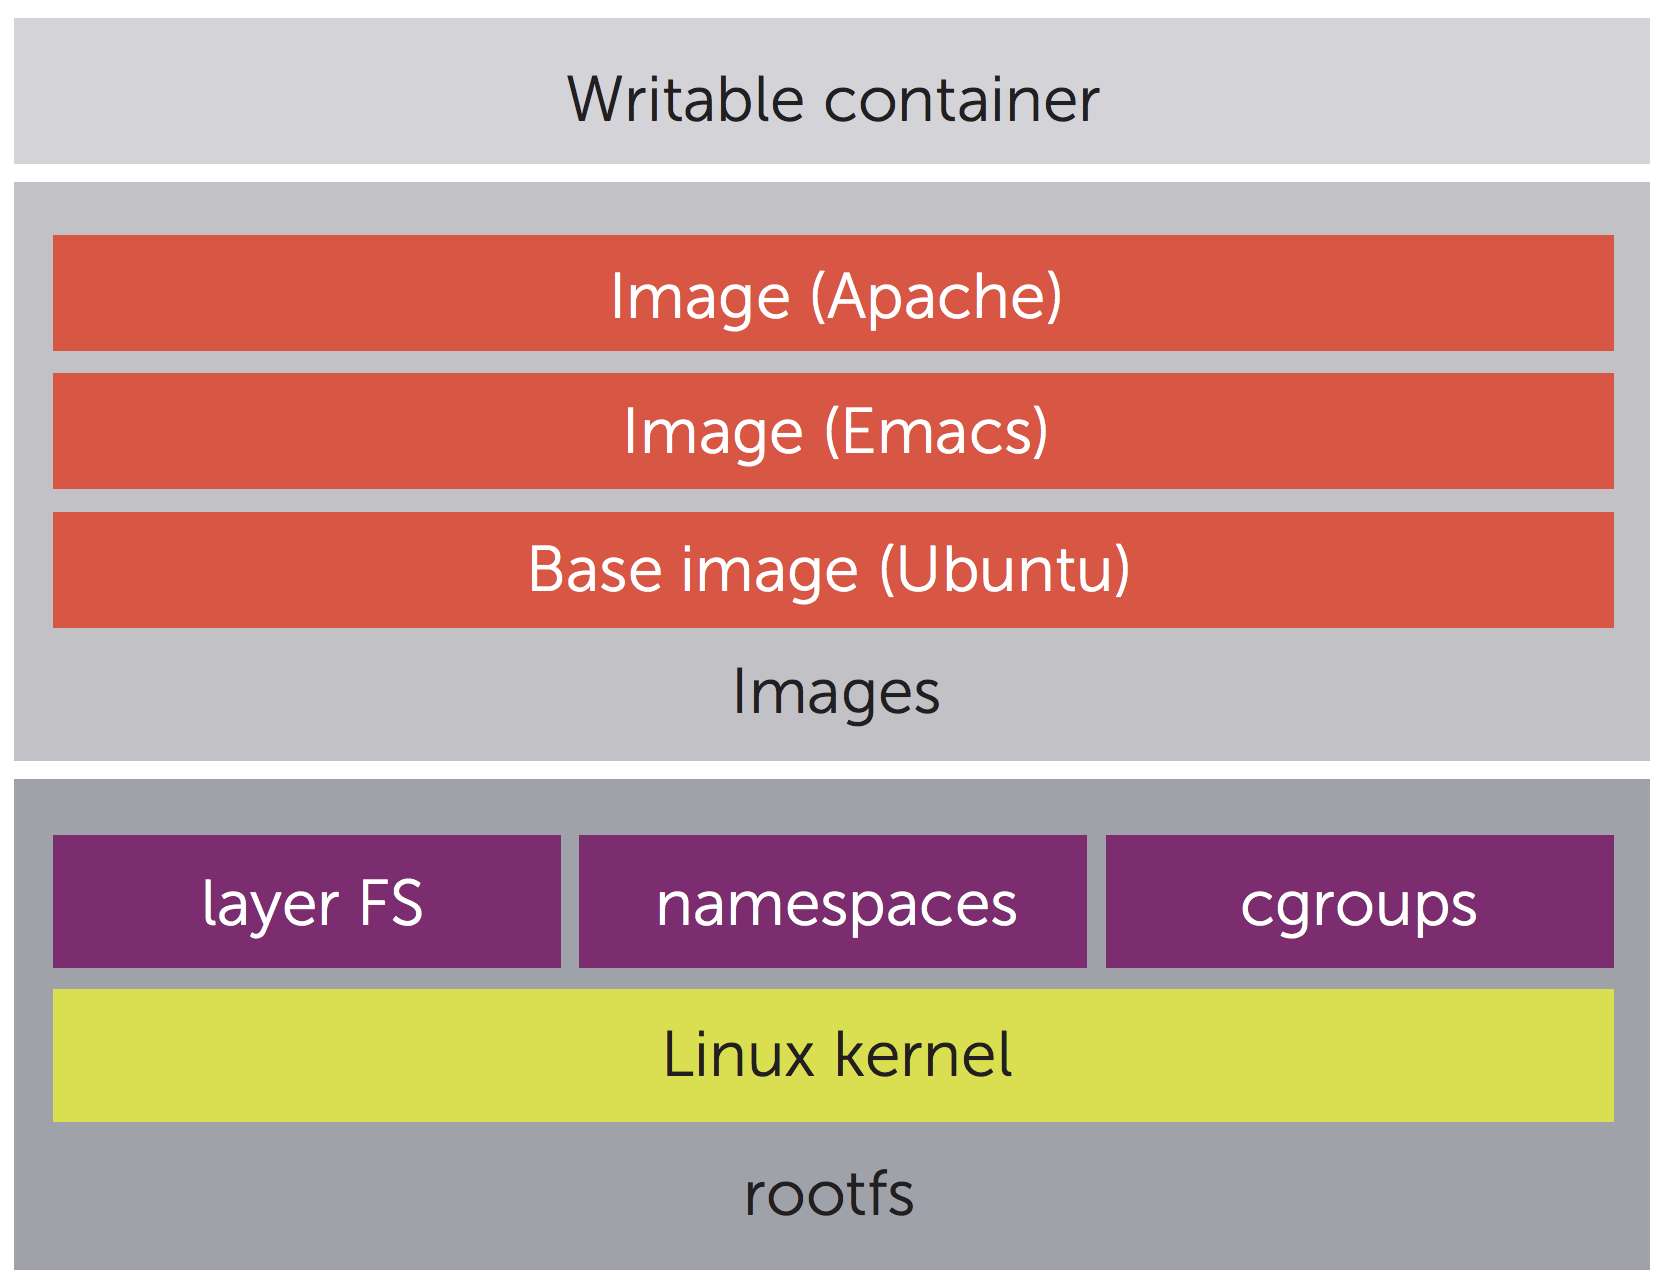
\includegraphics[width=0.5\textwidth]{chapter-background/docker-layers.png}
\end{figure}

\section{Container Orchestration}
Container technologies such as Docker offer advanced features to use containers in production. These solutions often offer deployment of applications limited to single machines. However, applications offered by  SaaS providers may include multiple different containers working together running on a cluster of nodes. Container orchestration (CO) systems allow deployment and management of containers at scale. Popular orchestration engines are Kubernetes, Docker Swarm and Mesos Marathon.
\subsection{Key capabilities of a container orchestration platform}
The task of a container orchestration (CO) platform is not limited to the initial deployment but the entire life-cycle of multiple containers. The goal of CO is to simplify cluster management while ensuring fault tolerance, availability, scalability and reliability. Allowing users to benefit from the complete potential of containers. In order to meet this goal, CO platform must at least offer the following key capabilities.~\cite{khan2017key}
\paragraph{Cluster state management and scheduling}
A cluster can be composed out of multiple virtualized or physical instances. Running containers on top of these instances and recover from failures requires a stable cluster. State management encapsulates various tasks such as flexible scheduling, re-partitioning of resources and data and propagating of dependent system changes.~\cite{khan2017key} 
\paragraph{High availability and fault tolerance}
A container orchestration platform must ensure high availability and fault tolerance in order to be useful for application developers. Most platforms therefor employ design principles of reliability engineering e.g., single point of failure elimination, failure detection or load balancing.~\cite{khan2017key}
\paragraph{Security}
Containers executing on top of the platform essentially form untrusted entities, with potentially malicious intentions, a high security standard is required. The standard should include: container images sanity check policies, access control for both containers and users, and techniques to minimize the container attack surface.~\cite{khan2017key}  
\paragraph{Simplified networking}
Containers must be able to communicate across nodes in  an efficient and secure manner. This requires the mapping of allocated host ports to containers. The overhead corresponding to this mapping intensifies at scale. The CO platform should thus provide a flexible, secure and scalable solution for networking.~\cite{khan2017key}
\paragraph{Service discovery}
The large number of services present in a cluster need to be able to communicate with each other. In traditional clusters services were handled as pets (i.e, having static names, IP addresses), however, in dynamic environments such as container orchestration platforms, they are regarded as cattle. The CO platform must provide mechanisms for addressing/labeling/grouping and service discovery.~\cite{khan2017key} 
\paragraph{Monitoring and governance}
The container orchestration platform needs to support traditional monitoring techniques such as logging, resource usage and network trace-routes. Monitoring must be possible at both the level of the underlying infrastructure and the containers themselves.~\cite{khan2017key}
\paragraph{Integrating for continuous integration and delivery}
Software development teams should be able to integrate the CO platform within their employed continuous integration and delivery (CI/CD) pipeline. The CO platform should contain mechanisms for rolling updates, rollbacks, etc.~\cite{khan2017key}


\subsection{Kubernetes}
Kubernetes~\cite{kubernetes}, commonly referred to as K8,  is one of the most popular and adopted orchestration systems. It is an open-source project led by Google. Kubernetes is Google's solution for the growing demand of container deployments by external developers in its public business cloud and is based upon its predecessors  Borg~\cite{verma2015large} and Omega~\cite{schwarzkopf2013omega} that have been used to schedule the internal Google workload. Its main design goal is formulated as:\textit{ "to make it easy to deploy and manage complex distributed systems, while still benefiting from the improved utilization that containers enable~\cite{Burns:2016:BOK:2930840.2890784}"}.  \\\\
\noindent To achieve the above stated goal Kubernetes introduces a number of concepts for both containers and cluster resources. It implements the infrastructure as code model  by provides an abstraction layer on top of the physical infrastructure~\cite{hermanns2015current}. It allows to setup and manage container infrastructure by the configuration of these introduced concepts via a REST API or declarative YAML configuration files. Below the most relevant concepts are introduced.
\subsubsection{Kubernetes concepts}
\textbf{Pods.}  A pod is the smallest unit of deployment within Kubernetes. It is a group of one or more containers that logically belong together.   A pod and thus its containers run on the same node. They share the same network, storage and context (Linux namespaces, cgroups). A pod gets assigned a unique IP address. Pods are not self-healing meaning when an error occurs within the pod or during scheduling. It will be deleted. Due to this short life cycle using a single pod resource and its assigned IP address for applications is impractical. Kubernetes handles this by employing controllers and services.~\cite{pods}\\\\
\textbf{Deployments.}  A Deployment controller manages a pod or a ReplicaSet of pods. A ReplicaSet allows pods to be replicated across multiple nodes. A Deployment object is used to specify the desired state of pods (e.g. number of replica's). A deployment, in addition, allows for declarative updates. These updates can be used to change the number of container replicas of a ReplicaSet or to update a specific container image within the pod.  The Deployment controller changes the actual state to the desired state described by the update.~\cite{deployments}
\\\\
\textbf{Services.}  Services offer a solution for the short life cycle of pods (and their IP addresses). Services within Kubernetes offer a manner to expose a ReplicaSet of Pods via a unique name, stable IP address, network policy and ports. To determine which set of pods is targeted by a service, Kubernetes employs a Label selector. Labels are the core grouping primitive of Kubernetes and unlike names and UIDs do not offer uniqueness.\\  A Service can be exposed outside the cluster by using an external load balancer or by specifying a NodePort. When using a Nodeport each node within the cluster will expose the port and forward request into the service.~\cite{services}
\\\\
\textbf{Namespaces.}  Namespaces allow to partition resources of a physical cluster among multiple user organizations. Each namespace gets a share of the resources of the cluster, via resource quotas. Resource quotas are supported for CPU, memory and persistent volumes.~\cite{namespaces-k8}
\\\\
\textbf{Resource limits.}  Kubernetes allows the allocation of compute resources of both containers and Namespaces by the means of resource limits. These limits can be soft (limit) and hard (request) limits. A Request specifies the quantity of resource that is guaranteed to the container. A limit specifies the maximum quantity allocated to the container. When the requested resource quantities of a container are less than its limit, the container may be allocated additional resources if there are unallocated resources available.  The current supported compute resources are CPU, memory and storage within the root partition of the local node. Within a Pod it is possible to specify both request and limit for each container. When request and limits are specified, the scheduler will use them for both scheduling and eviction (when node capacity is reached) decisions.~\cite{kubresources}
\subsubsection{Kubernetes architecture}
The basic architecture of Kubernetes is illustrated in Figure~\ref{fig:kubarch}. A client-server architecture is employed in which master and node setups are deployed on different machines. Below the different components that build up the architecture are briefly explained. 
\paragraph{API Server.} The API server is responsible for the configuration and validation of API objects (pods, deployments, services,...). It offers communication on cluster state via a REST interface for both components and administrators.~\cite{kubernetes-api-server}
\paragraph{Controller manager.} The controller manager is responsible for managing several core control loops part of Kubernetes. A control loop uses the API server to observe the shared state of the cluster and attempts to move to the desired state via configuration changes.~\cite{kubernetes-controller-manager}
\paragraph{Scheduler.} The task of assigning pods to nodes is the responsibility of the scheduler component.  The scheduler attempts to do a reasonable placement based on resource and quality of service requirements (e.g., not place a pod on a node with insufficient resources). It is  possible for users to control the placement of pods via NodeSelector tags or affinity and anti-affinity constraints in the configuration file.~\cite{kubernetes-pods-to-nodes,kubernetes-scheduler}
\\\\In addition it is possible to assign Quality of Service (QoS) classes to pods. These are used by Kubernetes in the decision process about scheduling and eviction of pods. Currently, Kubernetes supports three types of classes: guaranteed, burstable and best-effort. In decreasing order of priority (i.e., most likely to be killed in the case of resource shortages). The QoS classes are assigned to pods based on the presence of request and limit specifications of resources in their configuration files.~\cite{kubernetes-qos}


\paragraph{Kubelet.} The kubelet component is an agent running on each node. It is responsible for running and maintaining pods on its residing node. The set of maintained pods is described in the form of PodSpecs (mainly received via the API-server).~\cite{kubernetes-kubelet}
\paragraph{Kube-proxy.} The kube-proxy daemon provides a simple network proxy for the services on each node. It enables forwarding of requests to the correct containers and can provide primitive load balancing.~\cite{kubernetes-kubeproxy}
\begin{figure}[H]
\caption{Kubernetes architecture}
\centering
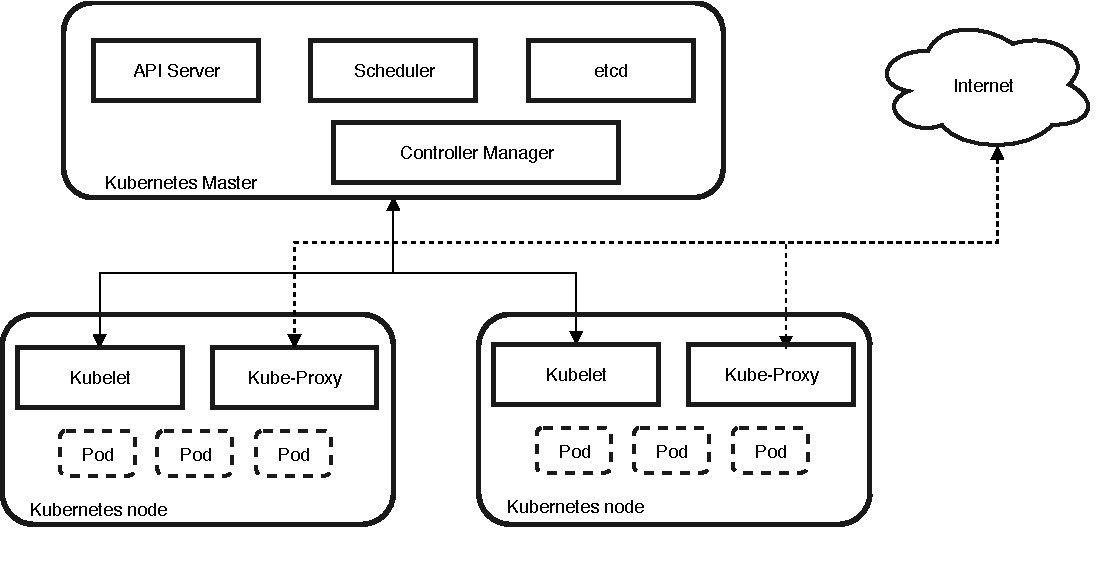
\includegraphics[width=0.8\textwidth]{chapter-background/kubernetes-architecture-diagram.pdf}
\label{fig:kubarch}
\end{figure}
 
 
 
 
 
 
 
 
 
 \section{Performance evaluation}
As discussed in previous sections, SaaS providers employ multi-tenancy to improve  cost efficiency and offer several performance guarantees to their customers in the form of SLOs. An unavoidable consequence of multi-tenancy is the need to support a growing number of users in a single system. Providers need to have a clear insight into the \textit{scalability} of their systems. However, scalability is a difficult thing to define, let alone quantify. Citing the words of  Dr. Neil J. Gunther:  \textit{"if you can't quantify it, you can't guarantee it"}.~\cite{perfdynamics}

\subsection{The Universal Scalability Law}
\label{section-USL}
Dr. Neil J. Gunther provides a formal definition of scalability: \textit{"scalability can be defined as a mathematical function, a relationship between independent and dependent variables (input and output)"~\cite{perfdynamics}}. The Universal Scalability Law (USL) by Dr. Neil J. Gunther is presented in Equation~\ref{USL}. It computes the relative capacity $C(N)$ at a load of $N$ users. Relative capacity is the normalized throughput.
\begin{equation}
\label{USL}
C(N) = \frac{\gamma~N}{1 + \alpha~(N-1) + \beta~N~(N-1)}
\end{equation}

The Universal Scalability Law incorporates factors that contribute to the sublinearly scalability of most systems. Namely, \textbf{concurrency} ($\gamma$), \textbf{contention} ($\alpha$) and \textbf{coherency} ($\beta$) as explained below. Their impact is visualized in Figure~\ref{fig:usl-impact}.

\begin{itemize}
    \item \textbf{Concurrency}($\gamma$): $\gamma$ defines the slope if the system was linearly scaling i.e., $C(N) = \gamma N$. It has been referred to as the \textit{coefficient of performance} by~\cite{schwarz2015practical}.
    \item \textbf{Contention} ($ \alpha $) : When scaling most systems parallelism while be limited at some point by contention (i.e., waiting or queuing for shared resources). The maximum speedup by parallelism is limited by the serialized portion ($\alpha$) of the work~\cite{schwarz2015practical}. 
    \item \textbf{Coherency} ($\beta$): created by crosstalk between components. Because crosstalk is possible between each pair of components in the system, the penalty grows quadratic $N(N-1)$.~\cite{schwarz2015practical}
    
\end{itemize}

\begin{figure}
    \centering
    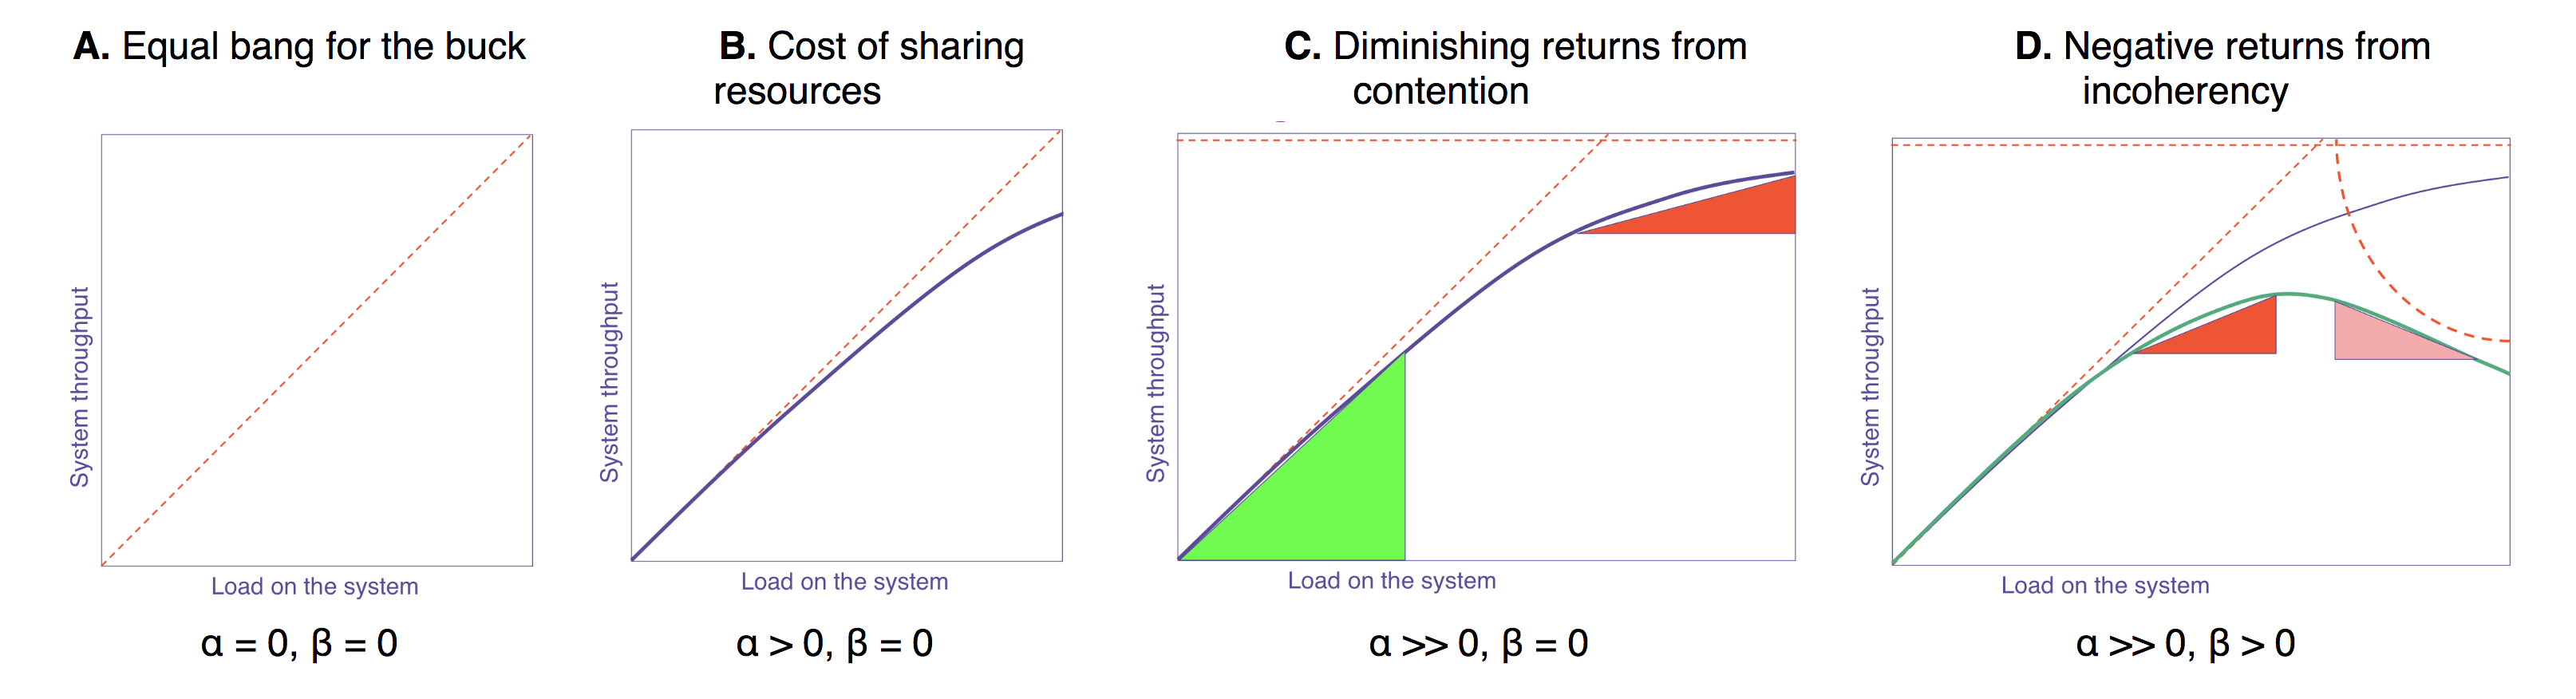
\includegraphics[width=1.1\textwidth]{chapter-evaluation/usl-impact}
    \caption{The impact of different USL coefficients on scalability.~\cite{perfdynamics}}
    \label{fig:usl-impact}
\end{figure}

\subsubsection{USL in practice}
USL can provide insights into a system's scalability pains via  values of the concurrency, contention and coherency coefficients. These can be obtained by collecting a dataset of measurements of the system, system load $N$ and corresponding throughput, and using a statistical technique such as nonlinear least square regression which fits the USL to the dataset.~\cite{schwarz2015practical,heyman2014scalability}

\subsection{Little's law}
\label{sec:little}
The Universal Law of Scalability serves as an alternative for the often less intuitive queuing models frequently used for modeling scalability. It omits the need to know the service time for every queue in the performance model in order to predict the response time or latency~\cite{perfdynamics}. Nevertheless, queuing theorem and its lemmas such as Little's Law can provide useful insights into performance modeling.\\\\
John D.C Little's Law~\cite{little2008little} states the following for stable systems: 
\begin{displayquote}
\textit{"The average number of items in a queuing system equals the average rate at which items arrive multiplied by the average time that an item spends in the system.\cite{little2008little}"}
\end{displayquote}
\begin{equation}
\label{littleslaw}
L = \lambda~W
\end{equation}
\begin{equation}
\label{llsys}
N = X~Rt
\end{equation}
Equation~\ref{littleslaw} shows Little's law, below its terms and its applicability to web services (Equation~\ref{llsys}) are explained:
\begin{itemize}
    \item \textbf{$L$}:  Average number of items in the system. For a web service this is represented by the average number of concurrent users in the system $N$.
    \item \textbf{$\lambda$}: Long-term average arrival rate of items in the system per time unit. Little's law assumes a stable system for which the arrival rate and exit rate are identical. In a web service this is represented by the throughput $X$.
    \item \textbf{$W$}: Average waiting time of an item in the system, queuing time and service time combined. This is represented by the response time $Rt$ or latency of a request in a web service. When dealing with a system involving think time (e.g., after the response from a web service, a user needs time to think about his/her next request), $(Rt + Zt)$ is used. 
\end{itemize}

\subsubsection{Workload generator validation}
Developers employ software tools (JMeter~\cite{jmeter}, Locust~\cite{locust}, etc.)  to simulate a workload and test the performance of a system. A workload is a set of actions that represent the behavior of a client in the system. It is part of the test plan stating the number of concurrent users $N$ executing the workload for a specified period of time.\\\\
The results of a performance test are typically expressed in throughput $X$ and response time $Rt$. Using Little's law it is possible to validate these results. For example, a test plan of 1000 concurrent users $N$ results in a throughput of 50 requests per second and an average response time of 15 seconds. Following Little's law, a concurrence of only 750 users was reached, instead of the specified 1000. Little's law can thus be used to check if a workload generator works as specified.\\\\
Alternatively, if the average throughput and response time for a production system are known, Little's law can be used to correctly draw up a test plan.

\subsubsection{Response time or latency?}
Performance can either be measured in throughput or latency, both are correct but offer a different point of view. System performance is typically expressed in throughput: "The system can handle a million operations per second". However, users care more about their personal experience with a system which is influenced by the average latency of their request.~\cite{schwarz2015practical} \\\\
Figure~\ref{fig:ls_vs_tp} shows the relation between the average latency and throughput of a database under increasing load $N$. In this case, latency is kept stable by increasing the throughput with the increasing load up to a certain point.  A bottleneck caps the throughput of the systems and by Little's law for an increasing load and constant throughput, the latency must increase.~\cite{latvsthrough} \\\\
However in other systems, as discussed in Section~\ref{section-USL}, an increasing load might induce a diminishing result on the system's throughput. Following Little's law a decreasing throughput results in a higher latency under the same load. \\\\
Thus, for stable systems by Little's law,  the USL can be reformulated in terms of latency instead of throughput. Equation~\ref{USL-2} shows this reformulation.~\cite{schwarz2015practical}
\begin{equation}
\label{USL-2}
Latency(N) = \frac{1 + \alpha~(N-1) + \beta~N~(N-1)}{\gamma}
\end{equation}


\begin{figure}[H]
    \centering
    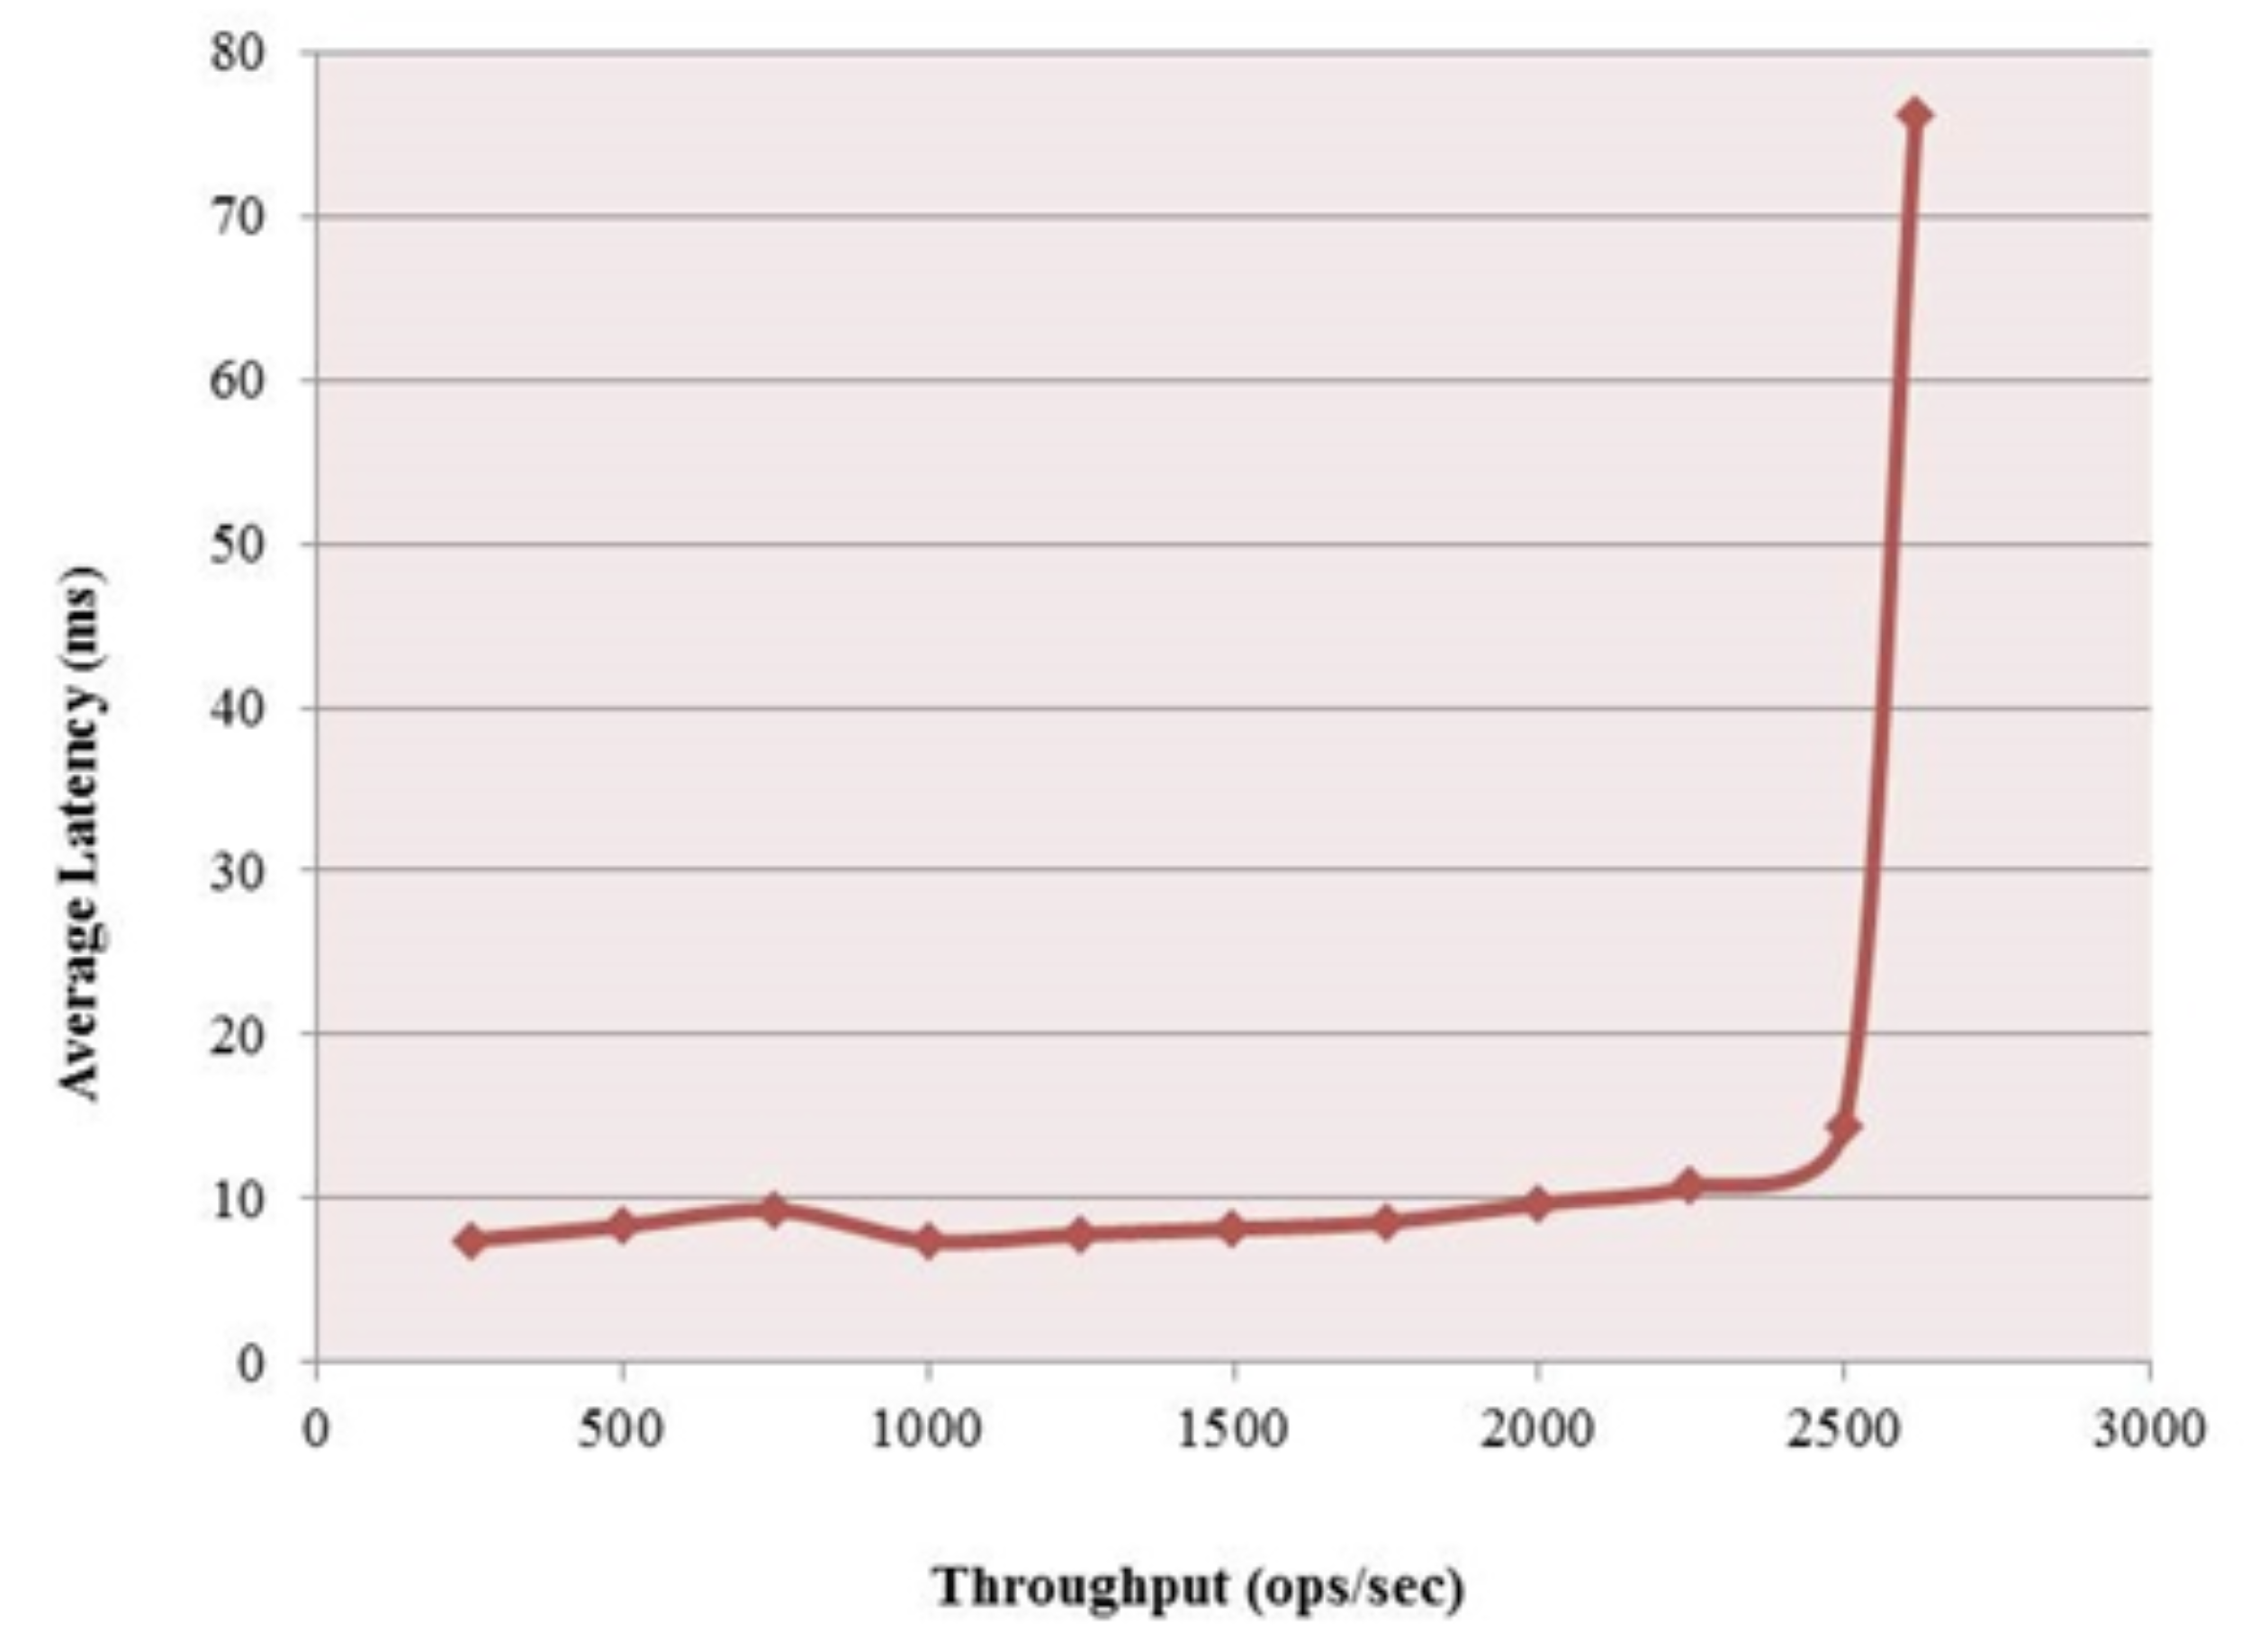
\includegraphics[width=0.8\textwidth]{chapter-evaluation/ls_vs_th}
    \caption{Relation average latency vs. throughput for database benchmark with increasing load.~\cite{latvsthrough}}
    \label{fig:ls_vs_tp}
\end{figure}
\chapter{Background}
\label{ch:background}
This chapter discusses relevant background material for the thesis. The concepts, explored in this chapter, further clarify the relevance of the thesis and serve as building blocks for the remaining chapters. Starting from the adoption of the cloud computing paradigm, the chapter elaborates on how concepts such as multi-tenancy and virtualization via containerization push the limits of efficient resource utilization. Next, an in-depth overview of the open-source container orchestration platform Kubernetes is provided. Lastly, insights are provided into the universal scalability law and the applicability of Little's law for performance testing.
\section{Cloud computing}
Companies try to minimize the total cost of ownership by moving to cloud computing or utility computing. The cloud computing paradigm enables on-demand access to a shared pool of configurable compute resources (software applications, system software and hardware infrastructure)~\cite{WalravenStefan2015PPmf}. A service provider can provision the required resources from the cloud with minimal effort.  Within this paradigm, services are offered in real time over the internet in three different models~\cite{MellPeter2010TNDo,rimal2009taxonomy}. 
\begin{itemize}
\item \textit{Infrastructure as a Service (IaaS)} in which access is offered to virtual machines, network, data storage and other fundamental computing resources. The customer is able to deploy arbitrary software using these resources.\\\\
Examples: Digital Ocean, Microsoft Azure and Amazon Elastic Compute Cloud (EC2).
\item \textit{Platform as a service (PaaS)} offers customers a platform enabling easy and efficient deployment of applications (at scale) while abstracting the complexity of managing the underlying infrastructure. PaaS allows customers to solely focus on the development of their application.\\\\
Examples: Google app engine, Microsoft Azure and Heroku.
\item \textit{Software as a service (SaaS) } allows customers to make use of a specific application developed by a SaaS provider. Compared to the traditional use of software, the management and deployment is the task of the SaaS provider. In this strategy, common resources and a single instance of both the application and underlying database are used to support multiple customers simultaneously. \\\\
Examples: Google apps and Salesforce.
\end{itemize}

\section{Multi-tenancy}
\label{multi-tenancy}
The software as a service (SaaS) model offers applications to customers as an on-demand service. Providers of these applications try to leverage economies of scale by employing a multi-tenancy architectural design principle. The goal of multi-tenancy is to minimize the total cost of ownership for the provider by maximizing the sharing of resources among multiple customers organizations, referred to as tenants.~\cite{Walraven2015b} 
\subsection{Service Level Agreements}
By moving their core business functions to an entrusted cloud provider, cloud customers give up control of the underlying compute resources. It is vital for these tenants to obtain certain guarantees on the service delivered by the provider. 
A Service Level Agreement (SLA) is a formal contract between the SaaS provider and the tenant specifying both properties of the provided service and the expected behavior of the tenant. An SLA typically also contains a set of Service Level Objectives (SLOs). An SLO is a measurable characteristic of the service. An SLO is typically related to performance constraints (latency, throughput and deadlines) or availability (uptime percentage) of the service. Within the specification of an SLA a trade-off must often be made between expressiveness and usability. The SLA must cover all the expectations of a customer while remaining simple to weight, verify, evaluated and enforce~\cite{dillon2010cloud}.  Some typical examples of SLOs are shown below: 
\begin{itemize}
\item The application has a monthly uptime percentage of 99.95\%.
\item If the arrival rate of the tenant workload < X requests/s then a throughput T is guaranteed.
\end{itemize}
\subsection{Challenges}
While the goal of multi-tenancy is promising, sharing a cluster of dynamically provisioned nodes between multiple tenants imposes a number of challenges and requirements~\cite{TruyenEddy2016Taca}. 
\begin{itemize}
\item Performance isolation: the activities of one tenant should not be able to influence the service level delivered to other tenants. This requirement should be achieved during normal system load and when an aggressive tenant violates the terms of the SLA. 
\item QoS differentiation: the performance guarantees specified by an SLA can be individually customized for each tenant. A SaaS provider should be able to offer different subscriptions.
\item Flexible resource allocation for improved server consolidation: a SaaS provider employs a multi-tenant architecture to achieve a lower operational cost. This is partially achieved by planning the required node capacity based on the actual resource usage of tenants instead of the theoretical required capacity.  This can be further aided by the use of request schedulers allowing to distinguish between normal, passive and aggressive tenants. 
\end{itemize}
\subsection{Strategies}
To achieve multi-tenancy different strategies, each offering different trade-offs concerning operational costs and upfront application engineering costs, can be employed by the SaaS-provider~\cite{WalravenS.2011Amlf}. The strategies are illustrated in Figure~\ref{muti-tenant-strategies}.
\begin{itemize}
\item Multi-tenancy can be achieved at the level of the \textit{operating system}. In this strategy, a virtualization technology can be used to partition compute resources among multiple virtual machines. Each tenant is assigned an application instance running on a dedicated virtual machine. This approach offers both a higher level of performance isolation and lower upfront engineering costs but suffers from an inefficient utilization of resources.
\item In \textit{middleware-level multi-tenancy} a middleware platform is used to enable sharing compute resources between multiple tenants at the level of the operating system. An application instance is deployed on top of the middleware platform for each tenant. By not replicating the operating system for each tenant a higher level of cost efficiency can be achieved but an increased complexity in managing resources and  performance isolation is introduced. By tackling these problems at the level of the middleware a part of the engineering complexity is shifted to this level.
\item The most efficient resource utilization can be achieved by sharing application instances between multiple tenants. In \textit{Application-level} multi-tenancy achieving performance isolation is done by the application itself thereby increasing the engineering complexity and costs.
\end{itemize}


\begin{figure}[H]

\caption{Different strategies to achieve multi-tenancy~\cite{WalravenS.2011Amlf}.\label{muti-tenant-strategies} }
\centering
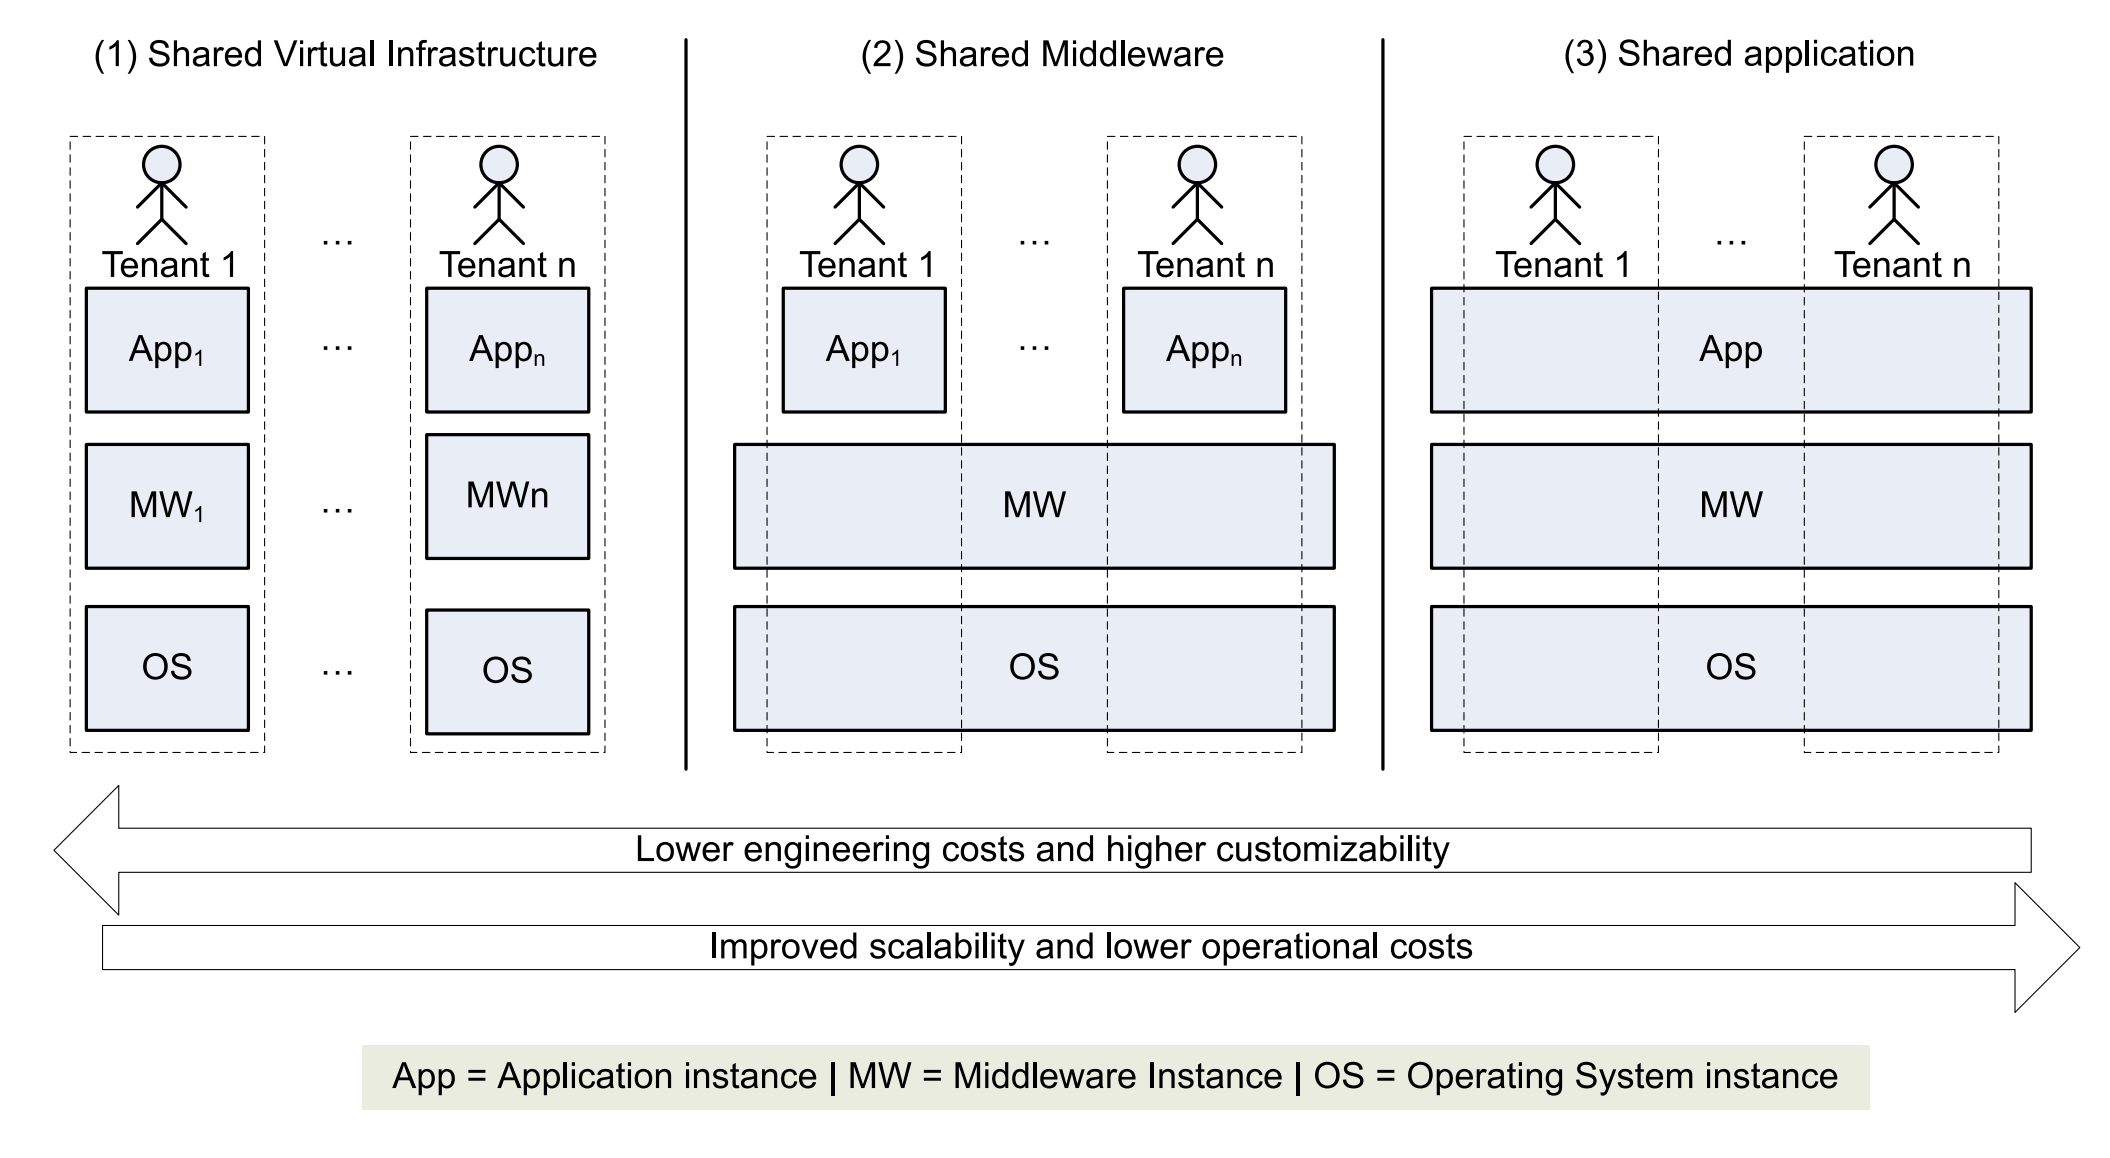
\includegraphics[width=0.65\textwidth]{chapter-background/muti-tenant-strategies.png}
\end{figure}


\section{Containerization}
Cloud providers rely on virtualization technology for the achievement of large-scale resource scaling. For more than a decade, virtual machines (VMs) have been the backbone of a provider's infrastructure offering hardware independence, availability, isolation and security~\cite{xavier2013performance}. More recently, containers a more lightweight virtualization technology have made advances in their multi-tenant capabilities and have seen an increase in adoption by providers~\cite{pahl2015containerization}. Both are discussed in this section.
\subsection{Virtualization technology}
In cloud environments, virtualization technology is used for flexible and dynamic allocation of physical resources to virtualized applications and to achieve multi-tenancy by sharing a physical server among multiple applications. In data centers virtualization is commonly used at the \textit{hardware level} and \textit{operating system level} to deploy and manage virtual machines and applications at scale~\cite{SharmaPrateek2016CaVM}. \\\\
Hardware level virtualization uses a hypervisor on a server to create virtual machines. Each virtual machine provides an abstraction of a physical machine and runs an independent operating system with applications. The hypervisor is responsible for resource allocation and performance isolation.\\\\
Operating system level virtualization allows resources to be shared at the level of the OS. Virtual machines running at the OS level are referred to as containers. Isolation, abstraction and resource allocation of containers is performed by the OS kernel of the host OS. By sharing the OS kernel among multiple containers, containers are regarded as a more lightweight virtualization technology. Containers only contain the application and its dependencies.\\\\
Linux containers (LXC)~\cite{lxc} employ different mechanisms of the Linux kernel to achieve resource isolation, namely control groups and namespaces.
\begin{itemize}
    \item \textbf{Cgroups}~\cite{cgroups} allow for fine-grained control of the allocation of system resources (CPU time, system memory, network bandwidth) among processes and process groups. For example, it is possible to limit or prioritize memory, CPU or I/O usage of different containers. 
    \item \textbf{Namespaces}~\cite{namespaces} allow for isolation of kernel resources among processes. A namespace makes a resource appear to be private and isolated for the container. The Linux kernel provides the following namespaces:  process ids, inter-process communication (IPC) mechanisms, network stack and mount points.
\end{itemize}
Linux containers (LXC) offers a lightweight implementation which performs at native speed and provides good isolation. However, while sharing a kernel between containers minimizes overhead, there are limitations in terms of the security environment.~\cite{dua2014virtualization}
\\\\
\noindent By offering virtualization at different levels, containers and VMs offer different trade-offs concerning performance isolation and performance. Research~\cite{SharmaPrateek2016CaVM} concludes that while containers offer closer to bare metal performance compared to VM, they offer worse performance isolation in multi-tenant environments. In addition, containers offer soft resource limits compared to the hard resource limits of virtual machines which allow for better server consolidation in over-commitment scenarios.  
\begin{figure}[h]
\caption{Container vs virtual machine.~\cite{container-vs-vms}}
\centering
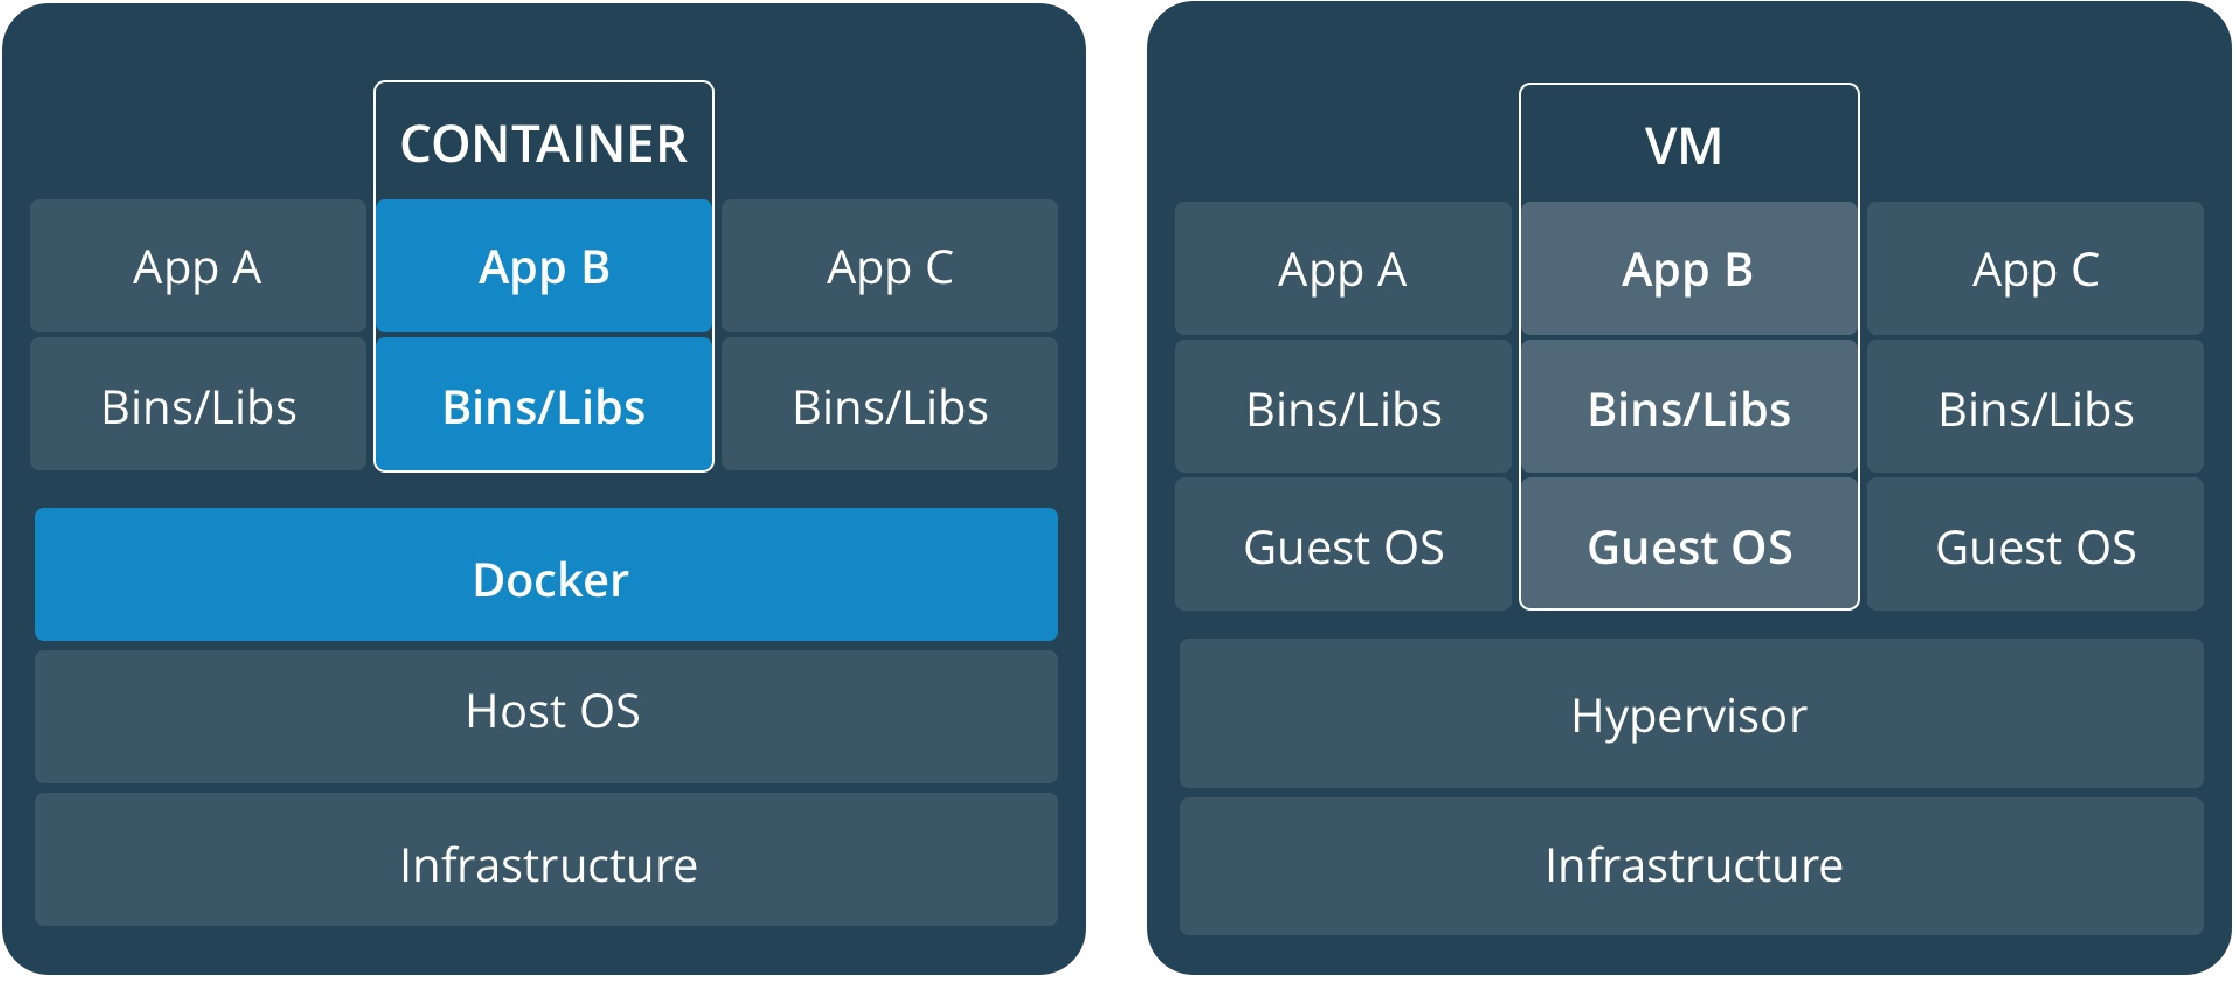
\includegraphics[width=0.8\textwidth]{chapter-background/containervsvm.pdf}
\end{figure}
\subsubsection{Docker}
Recently, thanks to Docker~\cite{dockersite}, containers have gained popularity and have been adopted into the software development process. However, Docker is not a new container technology, at its core it employs the kernel-level mechanisms of Linux containers (LXC), for which it defines a unified API~\cite{merkel2014docker}. In addition, the open-source Docker project offers a commandline-interface and daemon that offers easy packaging of applications in containers and the deployment of these containers.\\\\
To achieve this Docker introduces the concept of images. A container is represented by a lightweight image. A container image is a lightweight, executable package containing an application and its dependencies (runtime, libraries, environment variables, and config files). Virtual machines (VMs) can be seen as full, monolithic images. In particular,  Docker image consists of file-system layers stacked upon each other, as illustrated in Figure~\ref{docker-layers}. Only the top layer, the container itself, is writable, therefore it is state-full and executable. A container is thus composed out of layers of individual images built on top of a base image, allowing for easy extensibility.~\cite{pahl2015containerization} \\\\
A Docker image is specified by and build from a DockerFile. Images can be made easily accessible through Docker registries such as Dockerhub.\\
These images allow for easy and fast deployment of Docker containers across different operating systems and cloud provider stacks. Resulting in a game-changing technology for DevOps, system administrators and developers.
\begin{figure}[H]
\caption{Architecture of a container image. Images can be stacked upon each other using the cgroups and namespace extensions of a Linux kernel. The top container image is writable.~\cite{pahl2015containerization} \label{docker-layers}}
\centering
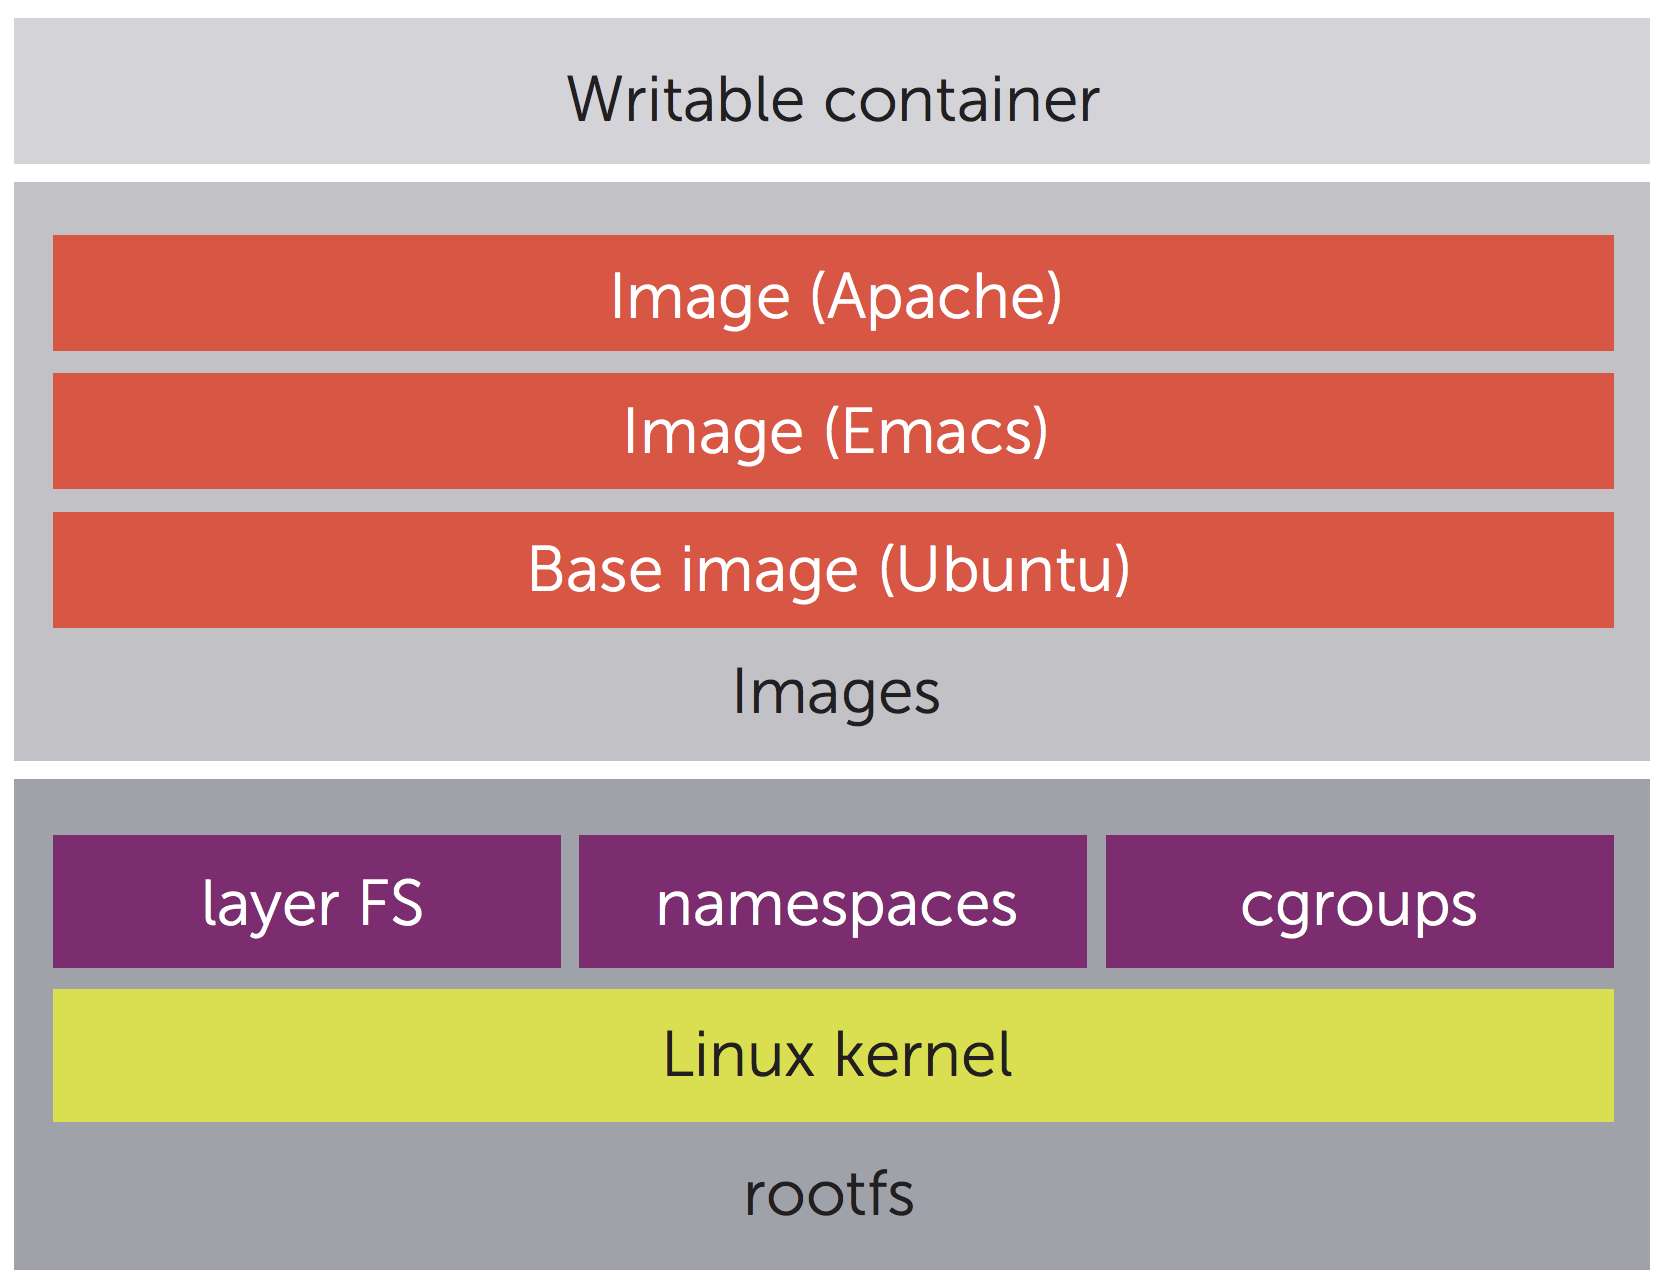
\includegraphics[width=0.5\textwidth]{chapter-background/docker-layers.png}
\end{figure}

\section{Container Orchestration}
Container technologies such as Docker offer advanced features to use containers in production. These solutions often offer deployment of applications limited to single machines. However, applications offered by  SaaS providers may include multiple different containers working together running on a cluster of nodes. Container orchestration (CO) systems allow deployment and management of containers at scale. Popular orchestration engines are Kubernetes, Docker Swarm and Mesos Marathon.
\subsection{Key capabilities of a container orchestration platform}
The task of a container orchestration (CO) platform is not limited to the initial deployment but the entire life-cycle of multiple containers. The goal of CO is to simplify cluster management while ensuring fault tolerance, availability, scalability and reliability. Allowing users to benefit from the complete potential of containers. In order to meet this goal, CO platform must at least offer the following key capabilities.~\cite{khan2017key}
\paragraph{Cluster state management and scheduling}
A cluster can be composed out of multiple virtualized or physical instances. Running containers on top of these instances and recover from failures requires a stable cluster. State management encapsulates various tasks such as flexible scheduling, re-partitioning of resources and data and propagating of dependent system changes.~\cite{khan2017key} 
\paragraph{High availability and fault tolerance}
A container orchestration platform must ensure high availability and fault tolerance in order to be useful for application developers. Most platforms therefor employ design principles of reliability engineering e.g., single point of failure elimination, failure detection or load balancing.~\cite{khan2017key}
\paragraph{Security}
Containers executing on top of the platform essentially form untrusted entities, with potentially malicious intentions, a high security standard is required. The standard should include: container images sanity check policies, access control for both containers and users, and techniques to minimize the container attack surface.~\cite{khan2017key}  
\paragraph{Simplified networking}
Containers must be able to communicate across nodes in  an efficient and secure manner. This requires the mapping of allocated host ports to containers. The overhead corresponding to this mapping intensifies at scale. The CO platform should thus provide a flexible, secure and scalable solution for networking.~\cite{khan2017key}
\paragraph{Service discovery}
The large number of services present in a cluster need to be able to communicate with each other. In traditional clusters services were handled as pets (i.e, having static names, IP addresses), however, in dynamic environments such as container orchestration platforms, they are regarded as cattle. The CO platform must provide mechanisms for addressing/labeling/grouping and service discovery.~\cite{khan2017key} 
\paragraph{Monitoring and governance}
The container orchestration platform needs to support traditional monitoring techniques such as logging, resource usage and network trace-routes. Monitoring must be possible at both the level of the underlying infrastructure and the containers themselves.~\cite{khan2017key}
\paragraph{Integrating for continuous integration and delivery}
Software development teams should be able to integrate the CO platform within their employed continuous integration and delivery (CI/CD) pipeline. The CO platform should contain mechanisms for rolling updates, rollbacks, etc.~\cite{khan2017key}


\subsection{Kubernetes}
Kubernetes~\cite{kubernetes}, commonly referred to as K8,  is one of the most popular and adopted orchestration systems. It is an open-source project led by Google. Kubernetes is Google's solution for the growing demand of container deployments by external developers in its public business cloud and is based upon its predecessors  Borg~\cite{verma2015large} and Omega~\cite{schwarzkopf2013omega} that have been used to schedule the internal Google workload. Its main design goal is formulated as:\textit{ "to make it easy to deploy and manage complex distributed systems, while still benefiting from the improved utilization that containers enable~\cite{Burns:2016:BOK:2930840.2890784}"}.  \\\\
\noindent To achieve the above stated goal Kubernetes introduces a number of concepts for both containers and cluster resources. It implements the infrastructure as code model  by provides an abstraction layer on top of the physical infrastructure~\cite{hermanns2015current}. It allows to setup and manage container infrastructure by the configuration of these introduced concepts via a REST API or declarative YAML configuration files. Below the most relevant concepts are introduced.
\subsubsection{Kubernetes concepts}
\textbf{Pods.}  A pod is the smallest unit of deployment within Kubernetes. It is a group of one or more containers that logically belong together.   A pod and thus its containers run on the same node. They share the same network, storage and context (Linux namespaces, cgroups). A pod gets assigned a unique IP address. Pods are not self-healing meaning when an error occurs within the pod or during scheduling. It will be deleted. Due to this short life cycle using a single pod resource and its assigned IP address for applications is impractical. Kubernetes handles this by employing controllers and services.~\cite{pods}\\\\
\textbf{Deployments.}  A Deployment controller manages a pod or a ReplicaSet of pods. A ReplicaSet allows pods to be replicated across multiple nodes. A Deployment object is used to specify the desired state of pods (e.g. number of replica's). A deployment, in addition, allows for declarative updates. These updates can be used to change the number of container replicas of a ReplicaSet or to update a specific container image within the pod.  The Deployment controller changes the actual state to the desired state described by the update.~\cite{deployments}
\\\\
\textbf{Services.}  Services offer a solution for the short life cycle of pods (and their IP addresses). Services within Kubernetes offer a manner to expose a ReplicaSet of Pods via a unique name, stable IP address, network policy and ports. To determine which set of pods is targeted by a service, Kubernetes employs a Label selector. Labels are the core grouping primitive of Kubernetes and unlike names and UIDs do not offer uniqueness.\\  A Service can be exposed outside the cluster by using an external load balancer or by specifying a NodePort. When using a Nodeport each node within the cluster will expose the port and forward request into the service.~\cite{services}
\\\\
\textbf{Namespaces.}  Namespaces allow to partition resources of a physical cluster among multiple user organizations. Each namespace gets a share of the resources of the cluster, via resource quotas. Resource quotas are supported for CPU, memory and persistent volumes.~\cite{namespaces-k8}
\\\\
\textbf{Resource limits.}  Kubernetes allows the allocation of compute resources of both containers and Namespaces by the means of resource limits. These limits can be soft (limit) and hard (request) limits. A Request specifies the quantity of resource that is guaranteed to the container. A limit specifies the maximum quantity allocated to the container. When the requested resource quantities of a container are less than its limit, the container may be allocated additional resources if there are unallocated resources available.  The current supported compute resources are CPU, memory and storage within the root partition of the local node. Within a Pod it is possible to specify both request and limit for each container. When request and limits are specified, the scheduler will use them for both scheduling and eviction (when node capacity is reached) decisions.~\cite{kubresources}
\subsubsection{Kubernetes architecture}
The basic architecture of Kubernetes is illustrated in Figure~\ref{fig:kubarch}. A client-server architecture is employed in which master and node setups are deployed on different machines. Below the different components that build up the architecture are briefly explained. 
\paragraph{API Server.} The API server is responsible for the configuration and validation of API objects (pods, deployments, services,...). It offers communication on cluster state via a REST interface for both components and administrators.~\cite{kubernetes-api-server}
\paragraph{Controller manager.} The controller manager is responsible for managing several core control loops part of Kubernetes. A control loop uses the API server to observe the shared state of the cluster and attempts to move to the desired state via configuration changes.~\cite{kubernetes-controller-manager}
\paragraph{Scheduler.} The task of assigning pods to nodes is the responsibility of the scheduler component.  The scheduler attempts to do a reasonable placement based on resource and quality of service requirements (e.g., not place a pod on a node with insufficient resources). It is  possible for users to control the placement of pods via NodeSelector tags or affinity and anti-affinity constraints in the configuration file.~\cite{kubernetes-pods-to-nodes,kubernetes-scheduler}
\\\\In addition it is possible to assign Quality of Service (QoS) classes to pods. These are used by Kubernetes in the decision process about scheduling and eviction of pods. Currently, Kubernetes supports three types of classes: guaranteed, burstable and best-effort. In decreasing order of priority (i.e., most likely to be killed in the case of resource shortages). The QoS classes are assigned to pods based on the presence of request and limit specifications of resources in their configuration files.~\cite{kubernetes-qos}


\paragraph{Kubelet.} The kubelet component is an agent running on each node. It is responsible for running and maintaining pods on its residing node. The set of maintained pods is described in the form of PodSpecs (mainly received via the API-server).~\cite{kubernetes-kubelet}
\paragraph{Kube-proxy.} The kube-proxy daemon provides a simple network proxy for the services on each node. It enables forwarding of requests to the correct containers and can provide primitive load balancing.~\cite{kubernetes-kubeproxy}
\begin{figure}[H]
\caption{Kubernetes architecture}
\centering
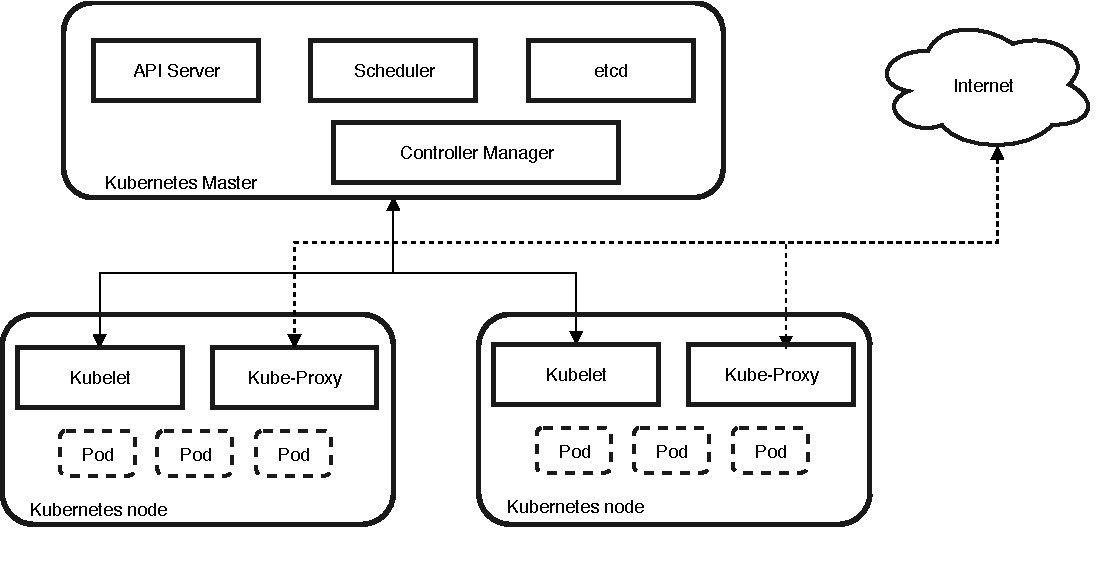
\includegraphics[width=0.8\textwidth]{chapter-background/kubernetes-architecture-diagram.pdf}
\label{fig:kubarch}
\end{figure}
 
 
 
 
 
 
 
 
 
 \section{Performance evaluation}
As discussed in previous sections, SaaS providers employ multi-tenancy to improve  cost efficiency and offer several performance guarantees to their customers in the form of SLOs. An unavoidable consequence of multi-tenancy is the need to support a growing number of users in a single system. Providers need to have a clear insight into the \textit{scalability} of their systems. However, scalability is a difficult thing to define, let alone quantify. Citing the words of  Dr. Neil J. Gunther:  \textit{"if you can't quantify it, you can't guarantee it"}.~\cite{perfdynamics}

\subsection{The Universal Scalability Law}
\label{section-USL}
Dr. Neil J. Gunther provides a formal definition of scalability: \textit{"scalability can be defined as a mathematical function, a relationship between independent and dependent variables (input and output)"~\cite{perfdynamics}}. The Universal Scalability Law (USL) by Dr. Neil J. Gunther is presented in Equation~\ref{USL}. It computes the relative capacity $C(N)$ at a load of $N$ users. Relative capacity is the normalized throughput.
\begin{equation}
\label{USL}
C(N) = \frac{\gamma~N}{1 + \alpha~(N-1) + \beta~N~(N-1)}
\end{equation}

The Universal Scalability Law incorporates factors that contribute to the sublinearly scalability of most systems. Namely, \textbf{concurrency} ($\gamma$), \textbf{contention} ($\alpha$) and \textbf{coherency} ($\beta$) as explained below. Their impact is visualized in Figure~\ref{fig:usl-impact}.

\begin{itemize}
    \item \textbf{Concurrency}($\gamma$): $\gamma$ defines the slope if the system was linearly scaling i.e., $C(N) = \gamma N$. It has been referred to as the \textit{coefficient of performance} by~\cite{schwarz2015practical}.
    \item \textbf{Contention} ($ \alpha $) : When scaling most systems parallelism while be limited at some point by contention (i.e., waiting or queuing for shared resources). The maximum speedup by parallelism is limited by the serialized portion ($\alpha$) of the work~\cite{schwarz2015practical}. 
    \item \textbf{Coherency} ($\beta$): created by crosstalk between components. Because crosstalk is possible between each pair of components in the system, the penalty grows quadratic $N(N-1)$.~\cite{schwarz2015practical}
    
\end{itemize}

\begin{figure}
    \centering
    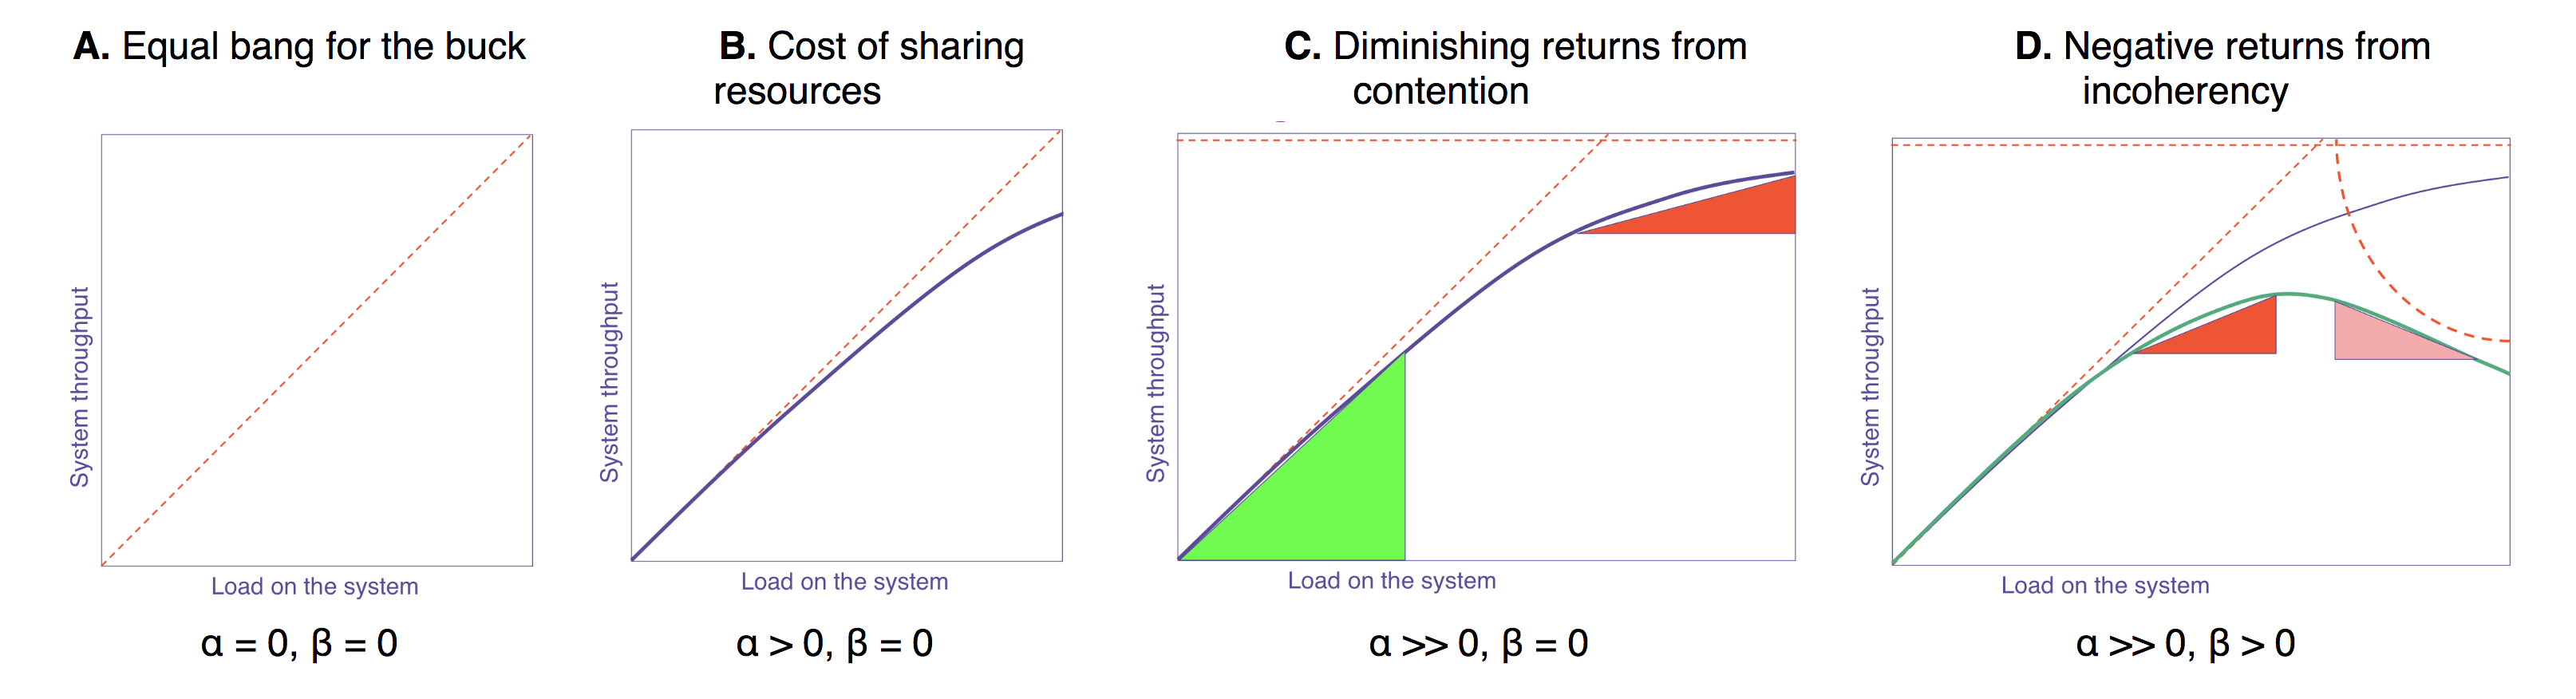
\includegraphics[width=1.1\textwidth]{chapter-evaluation/usl-impact}
    \caption{The impact of different USL coefficients on scalability.~\cite{perfdynamics}}
    \label{fig:usl-impact}
\end{figure}

\subsubsection{USL in practice}
USL can provide insights into a system's scalability pains via  values of the concurrency, contention and coherency coefficients. These can be obtained by collecting a dataset of measurements of the system, system load $N$ and corresponding throughput, and using a statistical technique such as nonlinear least square regression which fits the USL to the dataset.~\cite{schwarz2015practical,heyman2014scalability}

\subsection{Little's law}
\label{sec:little}
The Universal Law of Scalability serves as an alternative for the often less intuitive queuing models frequently used for modeling scalability. It omits the need to know the service time for every queue in the performance model in order to predict the response time or latency~\cite{perfdynamics}. Nevertheless, queuing theorem and its lemmas such as Little's Law can provide useful insights into performance modeling.\\\\
John D.C Little's Law~\cite{little2008little} states the following for stable systems: 
\begin{displayquote}
\textit{"The average number of items in a queuing system equals the average rate at which items arrive multiplied by the average time that an item spends in the system.\cite{little2008little}"}
\end{displayquote}
\begin{equation}
\label{littleslaw}
L = \lambda~W
\end{equation}
\begin{equation}
\label{llsys}
N = X~Rt
\end{equation}
Equation~\ref{littleslaw} shows Little's law, below its terms and its applicability to web services (Equation~\ref{llsys}) are explained:
\begin{itemize}
    \item \textbf{$L$}:  Average number of items in the system. For a web service this is represented by the average number of concurrent users in the system $N$.
    \item \textbf{$\lambda$}: Long-term average arrival rate of items in the system per time unit. Little's law assumes a stable system for which the arrival rate and exit rate are identical. In a web service this is represented by the throughput $X$.
    \item \textbf{$W$}: Average waiting time of an item in the system, queuing time and service time combined. This is represented by the response time $Rt$ or latency of a request in a web service. When dealing with a system involving think time (e.g., after the response from a web service, a user needs time to think about his/her next request), $(Rt + Zt)$ is used. 
\end{itemize}

\subsubsection{Workload generator validation}
Developers employ software tools (JMeter~\cite{jmeter}, Locust~\cite{locust}, etc.)  to simulate a workload and test the performance of a system. A workload is a set of actions that represent the behavior of a client in the system. It is part of the test plan stating the number of concurrent users $N$ executing the workload for a specified period of time.\\\\
The results of a performance test are typically expressed in throughput $X$ and response time $Rt$. Using Little's law it is possible to validate these results. For example, a test plan of 1000 concurrent users $N$ results in a throughput of 50 requests per second and an average response time of 15 seconds. Following Little's law, a concurrence of only 750 users was reached, instead of the specified 1000. Little's law can thus be used to check if a workload generator works as specified.\\\\
Alternatively, if the average throughput and response time for a production system are known, Little's law can be used to correctly draw up a test plan.

\subsubsection{Response time or latency?}
Performance can either be measured in throughput or latency, both are correct but offer a different point of view. System performance is typically expressed in throughput: "The system can handle a million operations per second". However, users care more about their personal experience with a system which is influenced by the average latency of their request.~\cite{schwarz2015practical} \\\\
Figure~\ref{fig:ls_vs_tp} shows the relation between the average latency and throughput of a database under increasing load $N$. In this case, latency is kept stable by increasing the throughput with the increasing load up to a certain point.  A bottleneck caps the throughput of the systems and by Little's law for an increasing load and constant throughput, the latency must increase.~\cite{latvsthrough} \\\\
However in other systems, as discussed in Section~\ref{section-USL}, an increasing load might induce a diminishing result on the system's throughput. Following Little's law a decreasing throughput results in a higher latency under the same load. \\\\
Thus, for stable systems by Little's law,  the USL can be reformulated in terms of latency instead of throughput. Equation~\ref{USL-2} shows this reformulation.~\cite{schwarz2015practical}
\begin{equation}
\label{USL-2}
Latency(N) = \frac{1 + \alpha~(N-1) + \beta~N~(N-1)}{\gamma}
\end{equation}


\begin{figure}[H]
    \centering
    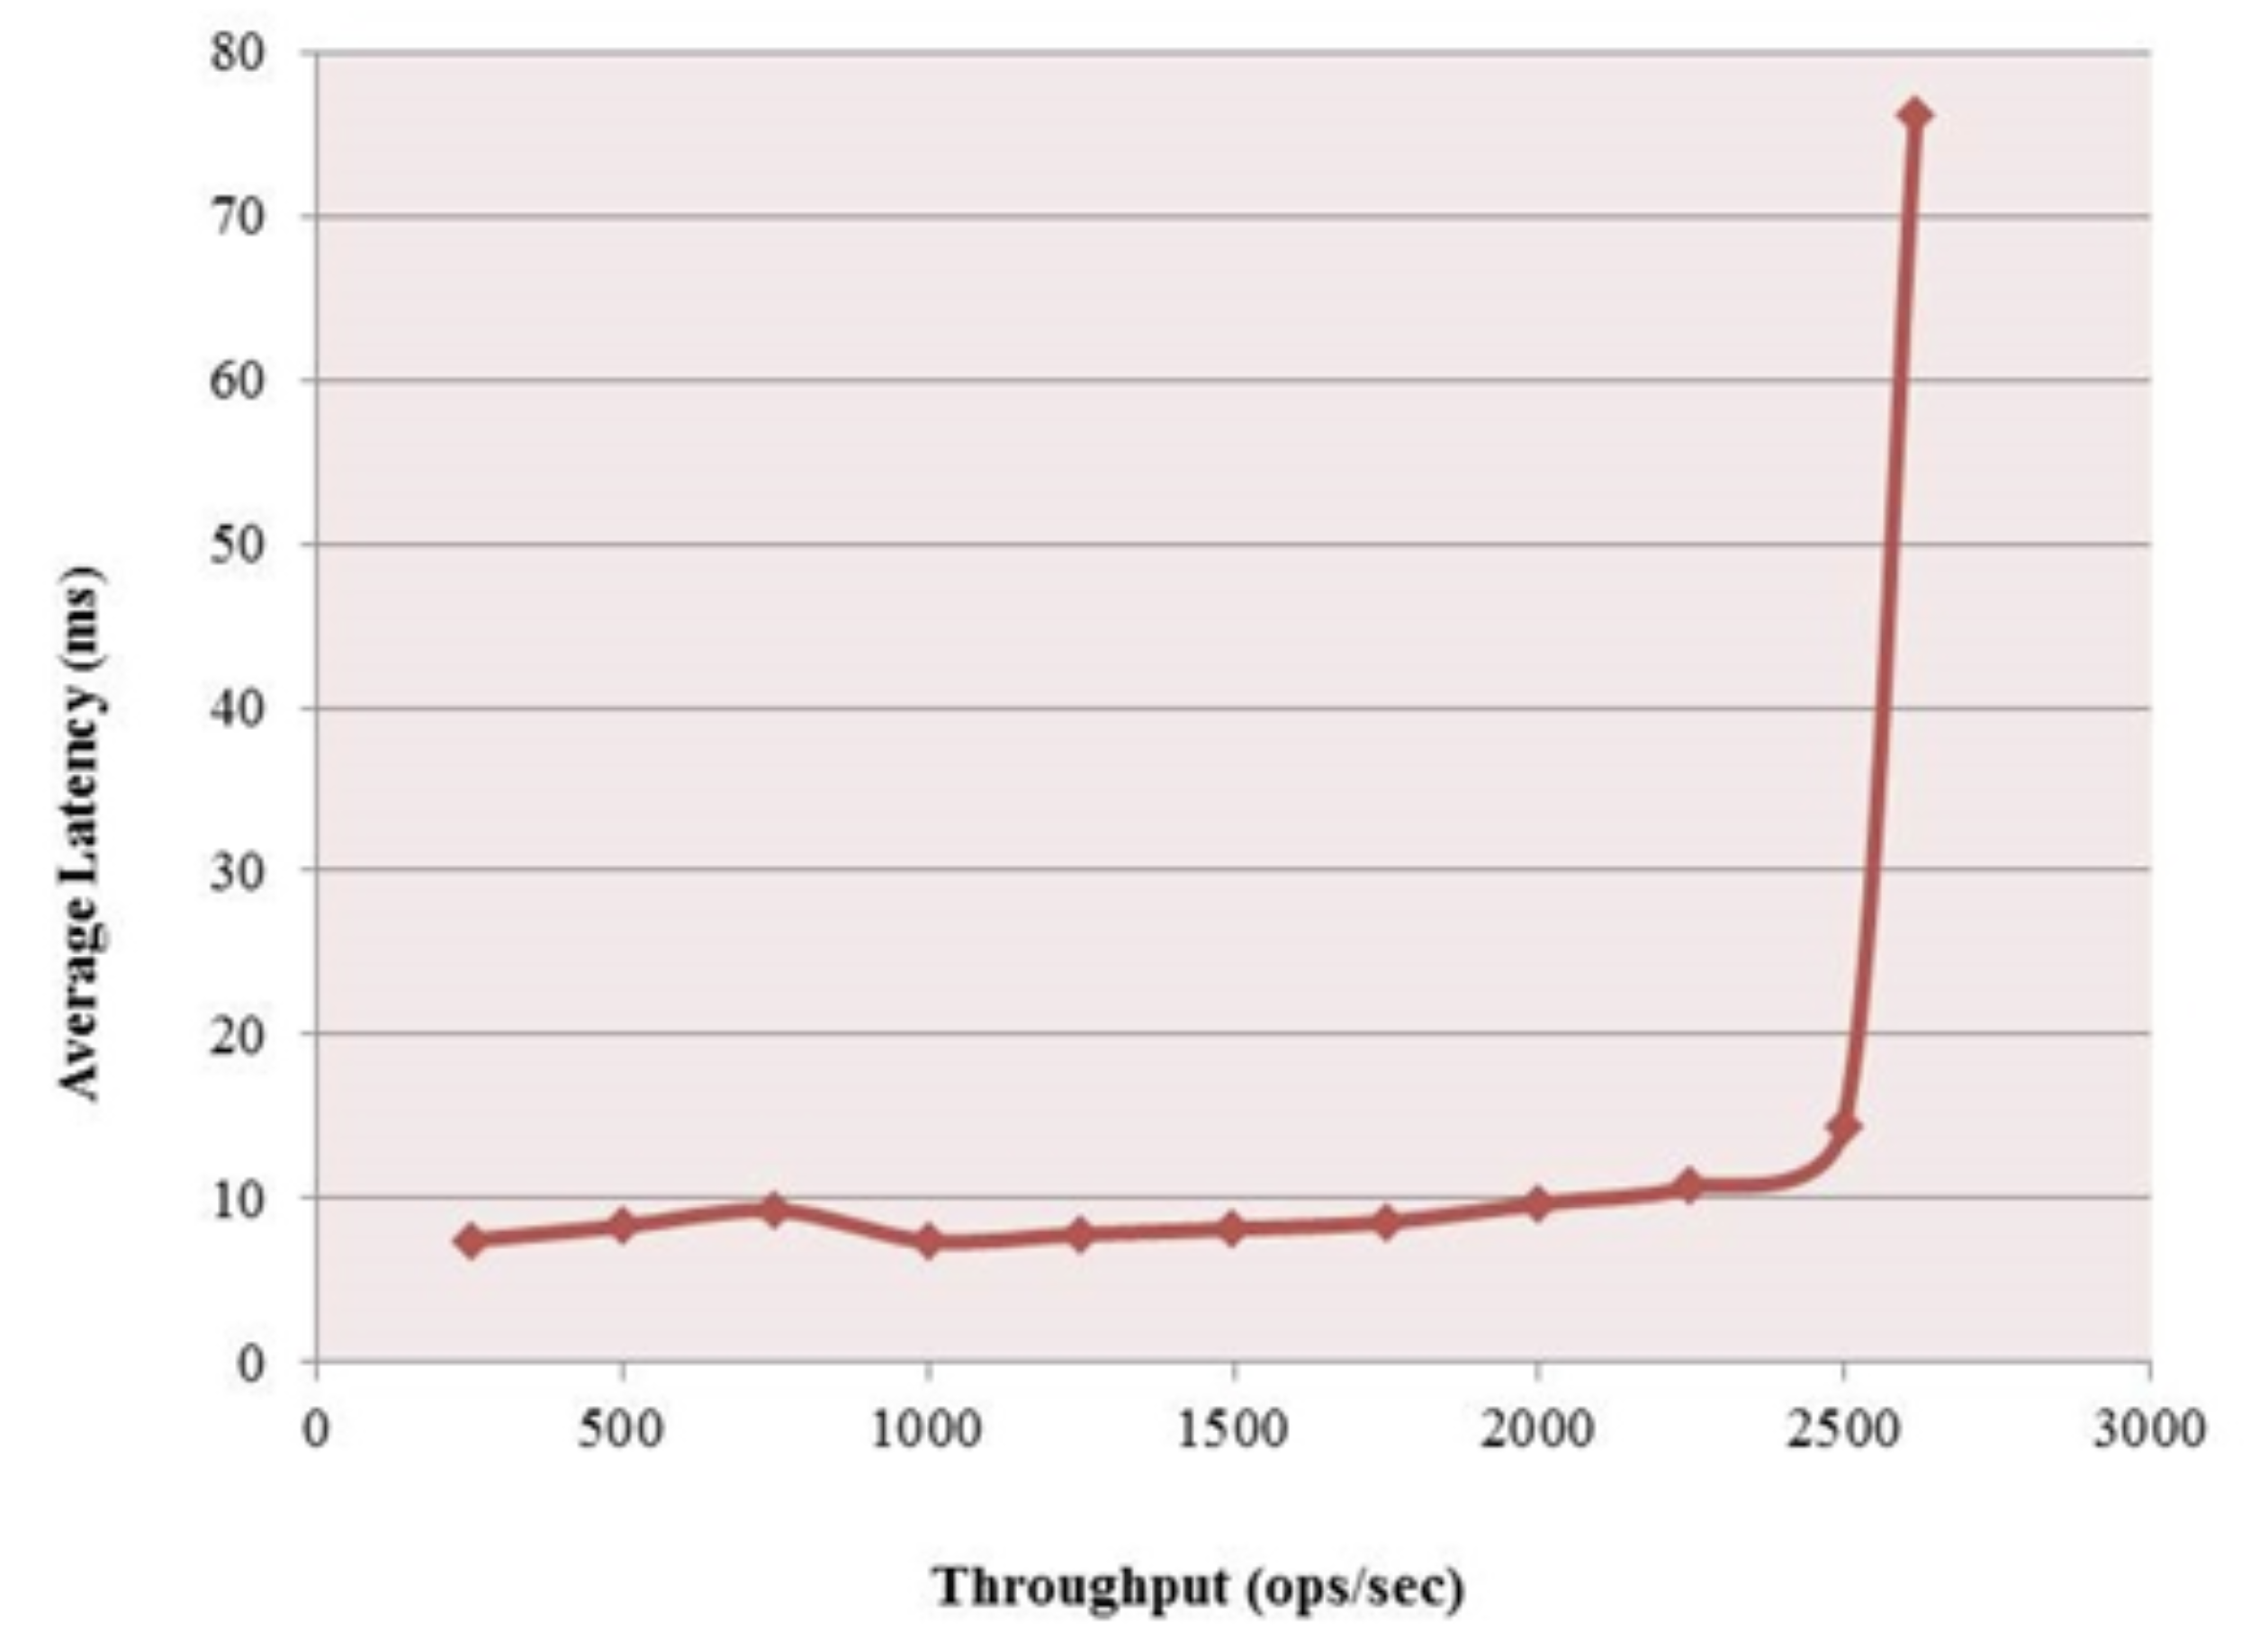
\includegraphics[width=0.8\textwidth]{chapter-evaluation/ls_vs_th}
    \caption{Relation average latency vs. throughput for database benchmark with increasing load.~\cite{latvsthrough}}
    \label{fig:ls_vs_tp}
\end{figure}
\chapter{Background}
\label{ch:background}
This chapter discusses relevant background material for the thesis. The concepts, explored in this chapter, further clarify the relevance of the thesis and serve as building blocks for the remaining chapters. Starting from the adoption of the cloud computing paradigm, the chapter elaborates on how concepts such as multi-tenancy and virtualization via containerization push the limits of efficient resource utilization. Next, an in-depth overview of the open-source container orchestration platform Kubernetes is provided. Lastly, insights are provided into the universal scalability law and the applicability of Little's law for performance testing.
\section{Cloud computing}
Companies try to minimize the total cost of ownership by moving to cloud computing or utility computing. The cloud computing paradigm enables on-demand access to a shared pool of configurable compute resources (software applications, system software and hardware infrastructure)~\cite{WalravenStefan2015PPmf}. A service provider can provision the required resources from the cloud with minimal effort.  Within this paradigm, services are offered in real time over the internet in three different models~\cite{MellPeter2010TNDo,rimal2009taxonomy}. 
\begin{itemize}
\item \textit{Infrastructure as a Service (IaaS)} in which access is offered to virtual machines, network, data storage and other fundamental computing resources. The customer is able to deploy arbitrary software using these resources.\\\\
Examples: Digital Ocean, Microsoft Azure and Amazon Elastic Compute Cloud (EC2).
\item \textit{Platform as a service (PaaS)} offers customers a platform enabling easy and efficient deployment of applications (at scale) while abstracting the complexity of managing the underlying infrastructure. PaaS allows customers to solely focus on the development of their application.\\\\
Examples: Google app engine, Microsoft Azure and Heroku.
\item \textit{Software as a service (SaaS) } allows customers to make use of a specific application developed by a SaaS provider. Compared to the traditional use of software, the management and deployment is the task of the SaaS provider. In this strategy, common resources and a single instance of both the application and underlying database are used to support multiple customers simultaneously. \\\\
Examples: Google apps and Salesforce.
\end{itemize}

\section{Multi-tenancy}
\label{multi-tenancy}
The software as a service (SaaS) model offers applications to customers as an on-demand service. Providers of these applications try to leverage economies of scale by employing a multi-tenancy architectural design principle. The goal of multi-tenancy is to minimize the total cost of ownership for the provider by maximizing the sharing of resources among multiple customers organizations, referred to as tenants.~\cite{Walraven2015b} 
\subsection{Service Level Agreements}
By moving their core business functions to an entrusted cloud provider, cloud customers give up control of the underlying compute resources. It is vital for these tenants to obtain certain guarantees on the service delivered by the provider. 
A Service Level Agreement (SLA) is a formal contract between the SaaS provider and the tenant specifying both properties of the provided service and the expected behavior of the tenant. An SLA typically also contains a set of Service Level Objectives (SLOs). An SLO is a measurable characteristic of the service. An SLO is typically related to performance constraints (latency, throughput and deadlines) or availability (uptime percentage) of the service. Within the specification of an SLA a trade-off must often be made between expressiveness and usability. The SLA must cover all the expectations of a customer while remaining simple to weight, verify, evaluated and enforce~\cite{dillon2010cloud}.  Some typical examples of SLOs are shown below: 
\begin{itemize}
\item The application has a monthly uptime percentage of 99.95\%.
\item If the arrival rate of the tenant workload < X requests/s then a throughput T is guaranteed.
\end{itemize}
\subsection{Challenges}
While the goal of multi-tenancy is promising, sharing a cluster of dynamically provisioned nodes between multiple tenants imposes a number of challenges and requirements~\cite{TruyenEddy2016Taca}. 
\begin{itemize}
\item Performance isolation: the activities of one tenant should not be able to influence the service level delivered to other tenants. This requirement should be achieved during normal system load and when an aggressive tenant violates the terms of the SLA. 
\item QoS differentiation: the performance guarantees specified by an SLA can be individually customized for each tenant. A SaaS provider should be able to offer different subscriptions.
\item Flexible resource allocation for improved server consolidation: a SaaS provider employs a multi-tenant architecture to achieve a lower operational cost. This is partially achieved by planning the required node capacity based on the actual resource usage of tenants instead of the theoretical required capacity.  This can be further aided by the use of request schedulers allowing to distinguish between normal, passive and aggressive tenants. 
\end{itemize}
\subsection{Strategies}
To achieve multi-tenancy different strategies, each offering different trade-offs concerning operational costs and upfront application engineering costs, can be employed by the SaaS-provider~\cite{WalravenS.2011Amlf}. The strategies are illustrated in Figure~\ref{muti-tenant-strategies}.
\begin{itemize}
\item Multi-tenancy can be achieved at the level of the \textit{operating system}. In this strategy, a virtualization technology can be used to partition compute resources among multiple virtual machines. Each tenant is assigned an application instance running on a dedicated virtual machine. This approach offers both a higher level of performance isolation and lower upfront engineering costs but suffers from an inefficient utilization of resources.
\item In \textit{middleware-level multi-tenancy} a middleware platform is used to enable sharing compute resources between multiple tenants at the level of the operating system. An application instance is deployed on top of the middleware platform for each tenant. By not replicating the operating system for each tenant a higher level of cost efficiency can be achieved but an increased complexity in managing resources and  performance isolation is introduced. By tackling these problems at the level of the middleware a part of the engineering complexity is shifted to this level.
\item The most efficient resource utilization can be achieved by sharing application instances between multiple tenants. In \textit{Application-level} multi-tenancy achieving performance isolation is done by the application itself thereby increasing the engineering complexity and costs.
\end{itemize}


\begin{figure}[H]

\caption{Different strategies to achieve multi-tenancy~\cite{WalravenS.2011Amlf}.\label{muti-tenant-strategies} }
\centering
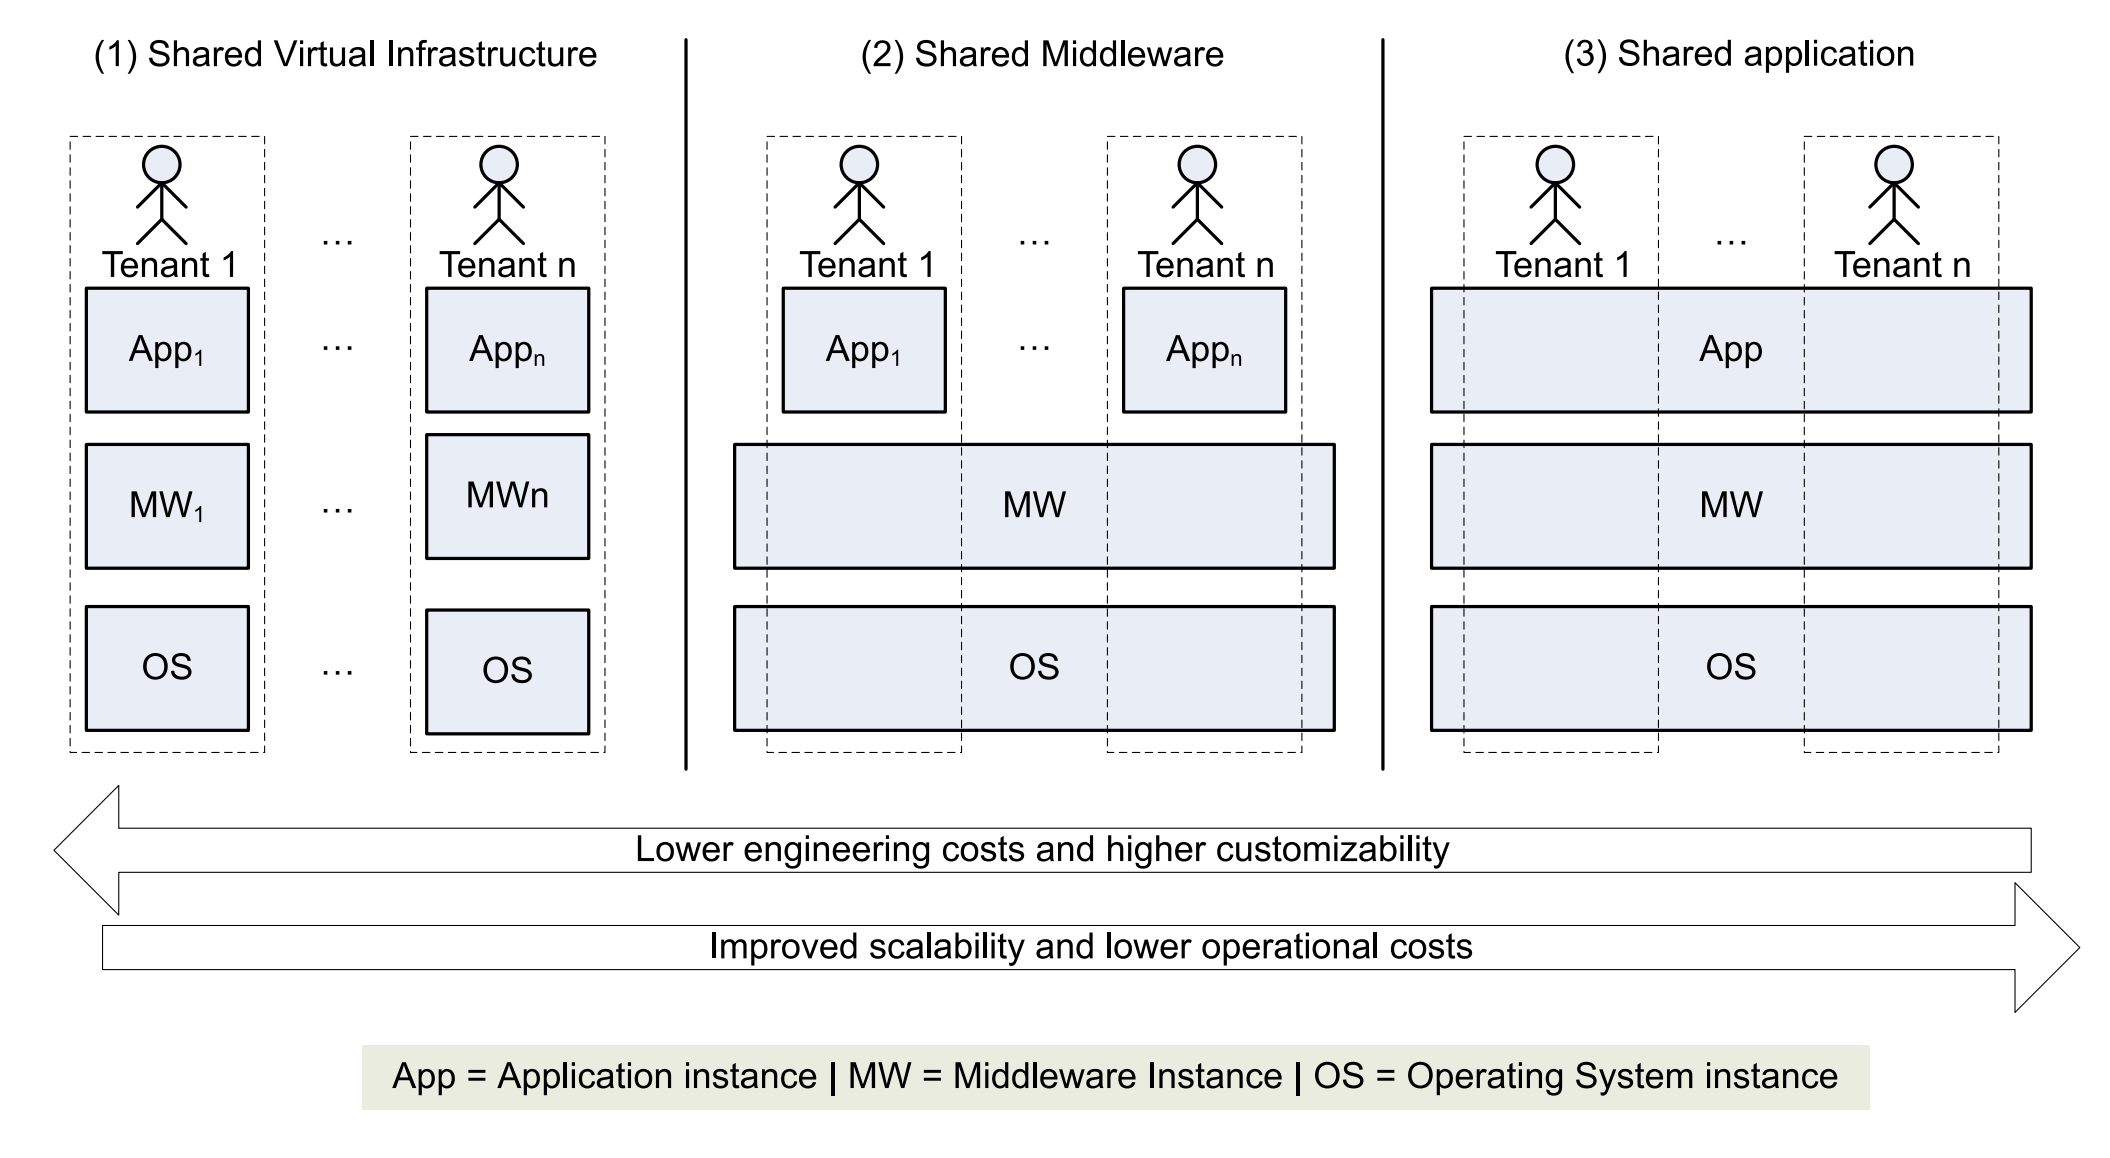
\includegraphics[width=0.65\textwidth]{chapter-background/muti-tenant-strategies.png}
\end{figure}


\section{Containerization}
Cloud providers rely on virtualization technology for the achievement of large-scale resource scaling. For more than a decade, virtual machines (VMs) have been the backbone of a provider's infrastructure offering hardware independence, availability, isolation and security~\cite{xavier2013performance}. More recently, containers a more lightweight virtualization technology have made advances in their multi-tenant capabilities and have seen an increase in adoption by providers~\cite{pahl2015containerization}. Both are discussed in this section.
\subsection{Virtualization technology}
In cloud environments, virtualization technology is used for flexible and dynamic allocation of physical resources to virtualized applications and to achieve multi-tenancy by sharing a physical server among multiple applications. In data centers virtualization is commonly used at the \textit{hardware level} and \textit{operating system level} to deploy and manage virtual machines and applications at scale~\cite{SharmaPrateek2016CaVM}. \\\\
Hardware level virtualization uses a hypervisor on a server to create virtual machines. Each virtual machine provides an abstraction of a physical machine and runs an independent operating system with applications. The hypervisor is responsible for resource allocation and performance isolation.\\\\
Operating system level virtualization allows resources to be shared at the level of the OS. Virtual machines running at the OS level are referred to as containers. Isolation, abstraction and resource allocation of containers is performed by the OS kernel of the host OS. By sharing the OS kernel among multiple containers, containers are regarded as a more lightweight virtualization technology. Containers only contain the application and its dependencies.\\\\
Linux containers (LXC)~\cite{lxc} employ different mechanisms of the Linux kernel to achieve resource isolation, namely control groups and namespaces.
\begin{itemize}
    \item \textbf{Cgroups}~\cite{cgroups} allow for fine-grained control of the allocation of system resources (CPU time, system memory, network bandwidth) among processes and process groups. For example, it is possible to limit or prioritize memory, CPU or I/O usage of different containers. 
    \item \textbf{Namespaces}~\cite{namespaces} allow for isolation of kernel resources among processes. A namespace makes a resource appear to be private and isolated for the container. The Linux kernel provides the following namespaces:  process ids, inter-process communication (IPC) mechanisms, network stack and mount points.
\end{itemize}
Linux containers (LXC) offers a lightweight implementation which performs at native speed and provides good isolation. However, while sharing a kernel between containers minimizes overhead, there are limitations in terms of the security environment.~\cite{dua2014virtualization}
\\\\
\noindent By offering virtualization at different levels, containers and VMs offer different trade-offs concerning performance isolation and performance. Research~\cite{SharmaPrateek2016CaVM} concludes that while containers offer closer to bare metal performance compared to VM, they offer worse performance isolation in multi-tenant environments. In addition, containers offer soft resource limits compared to the hard resource limits of virtual machines which allow for better server consolidation in over-commitment scenarios.  
\begin{figure}[h]
\caption{Container vs virtual machine.~\cite{container-vs-vms}}
\centering
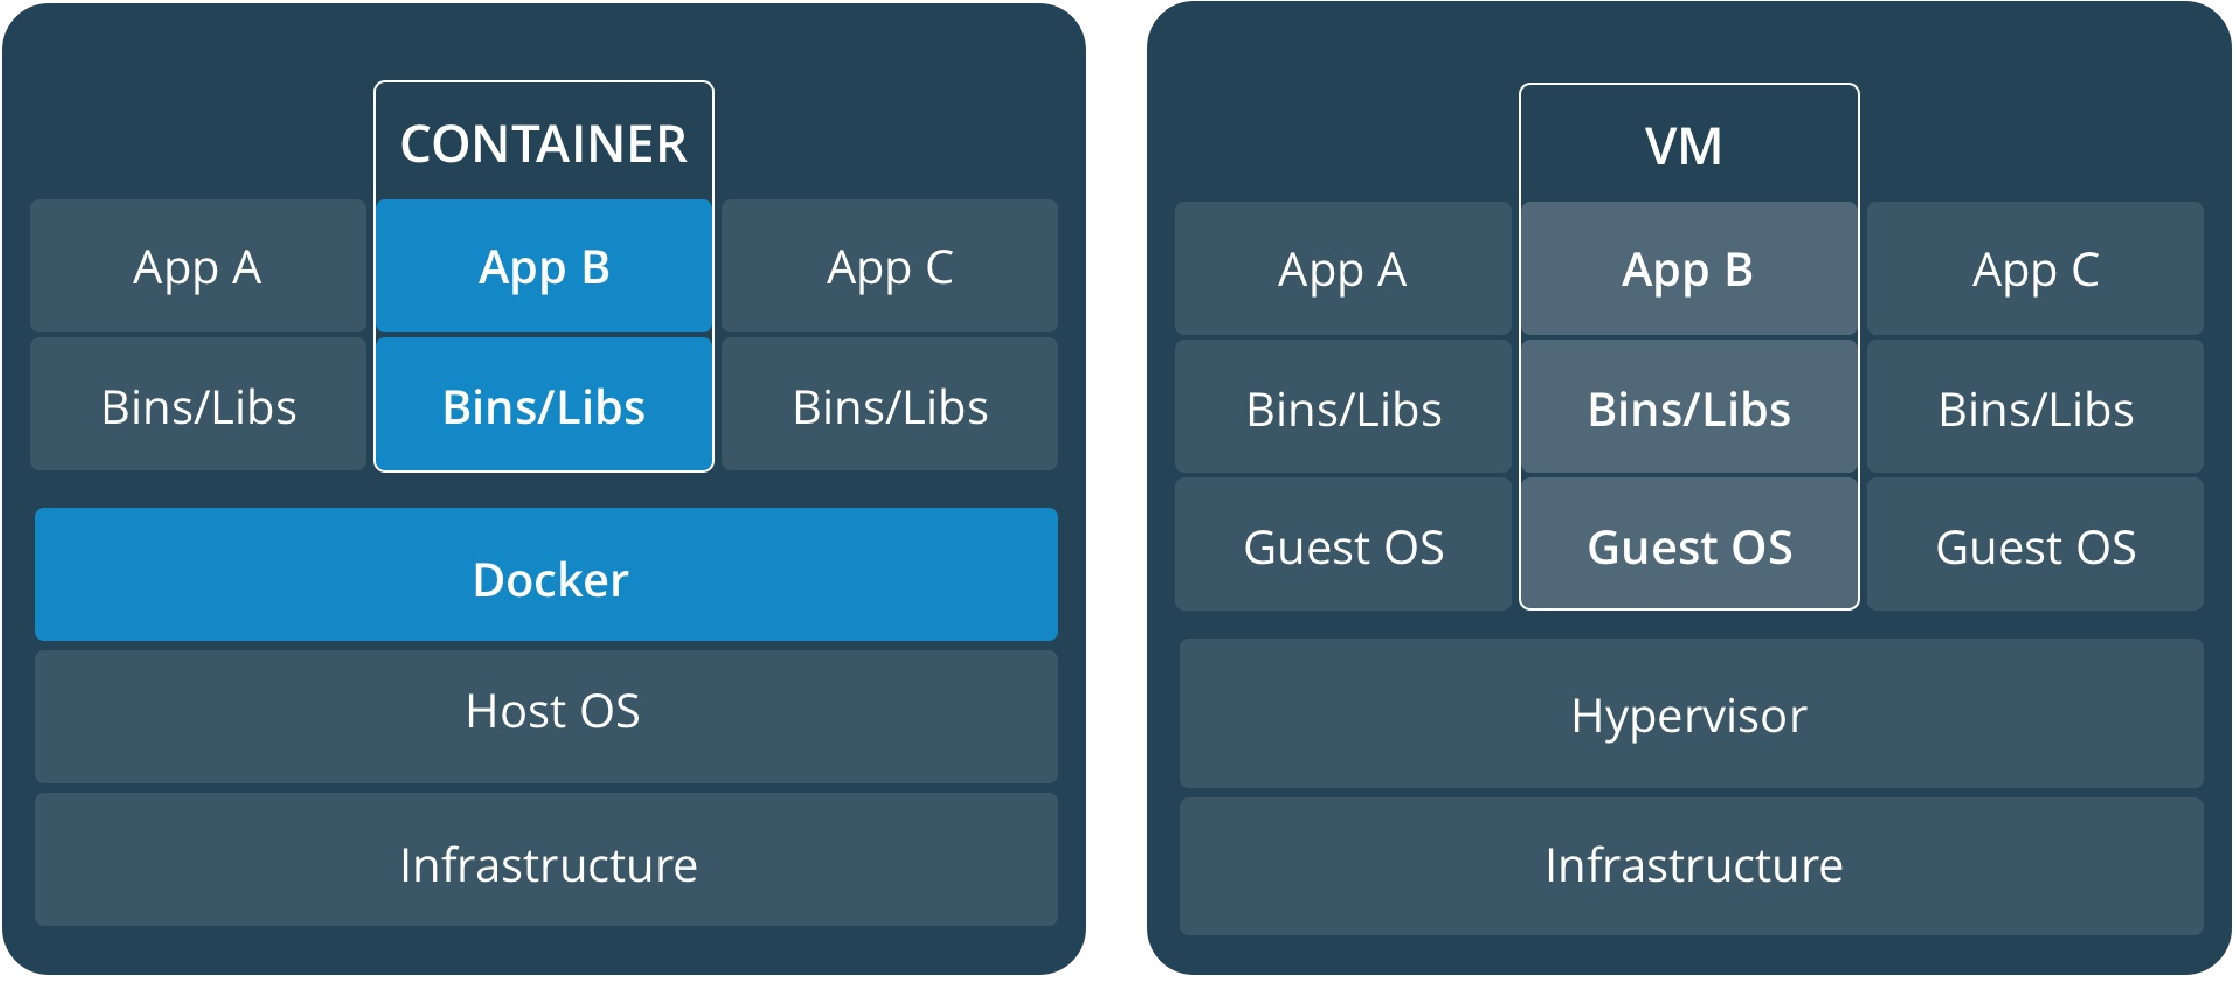
\includegraphics[width=0.8\textwidth]{chapter-background/containervsvm.pdf}
\end{figure}
\subsubsection{Docker}
Recently, thanks to Docker~\cite{dockersite}, containers have gained popularity and have been adopted into the software development process. However, Docker is not a new container technology, at its core it employs the kernel-level mechanisms of Linux containers (LXC), for which it defines a unified API~\cite{merkel2014docker}. In addition, the open-source Docker project offers a commandline-interface and daemon that offers easy packaging of applications in containers and the deployment of these containers.\\\\
To achieve this Docker introduces the concept of images. A container is represented by a lightweight image. A container image is a lightweight, executable package containing an application and its dependencies (runtime, libraries, environment variables, and config files). Virtual machines (VMs) can be seen as full, monolithic images. In particular,  Docker image consists of file-system layers stacked upon each other, as illustrated in Figure~\ref{docker-layers}. Only the top layer, the container itself, is writable, therefore it is state-full and executable. A container is thus composed out of layers of individual images built on top of a base image, allowing for easy extensibility.~\cite{pahl2015containerization} \\\\
A Docker image is specified by and build from a DockerFile. Images can be made easily accessible through Docker registries such as Dockerhub.\\
These images allow for easy and fast deployment of Docker containers across different operating systems and cloud provider stacks. Resulting in a game-changing technology for DevOps, system administrators and developers.
\begin{figure}[H]
\caption{Architecture of a container image. Images can be stacked upon each other using the cgroups and namespace extensions of a Linux kernel. The top container image is writable.~\cite{pahl2015containerization} \label{docker-layers}}
\centering
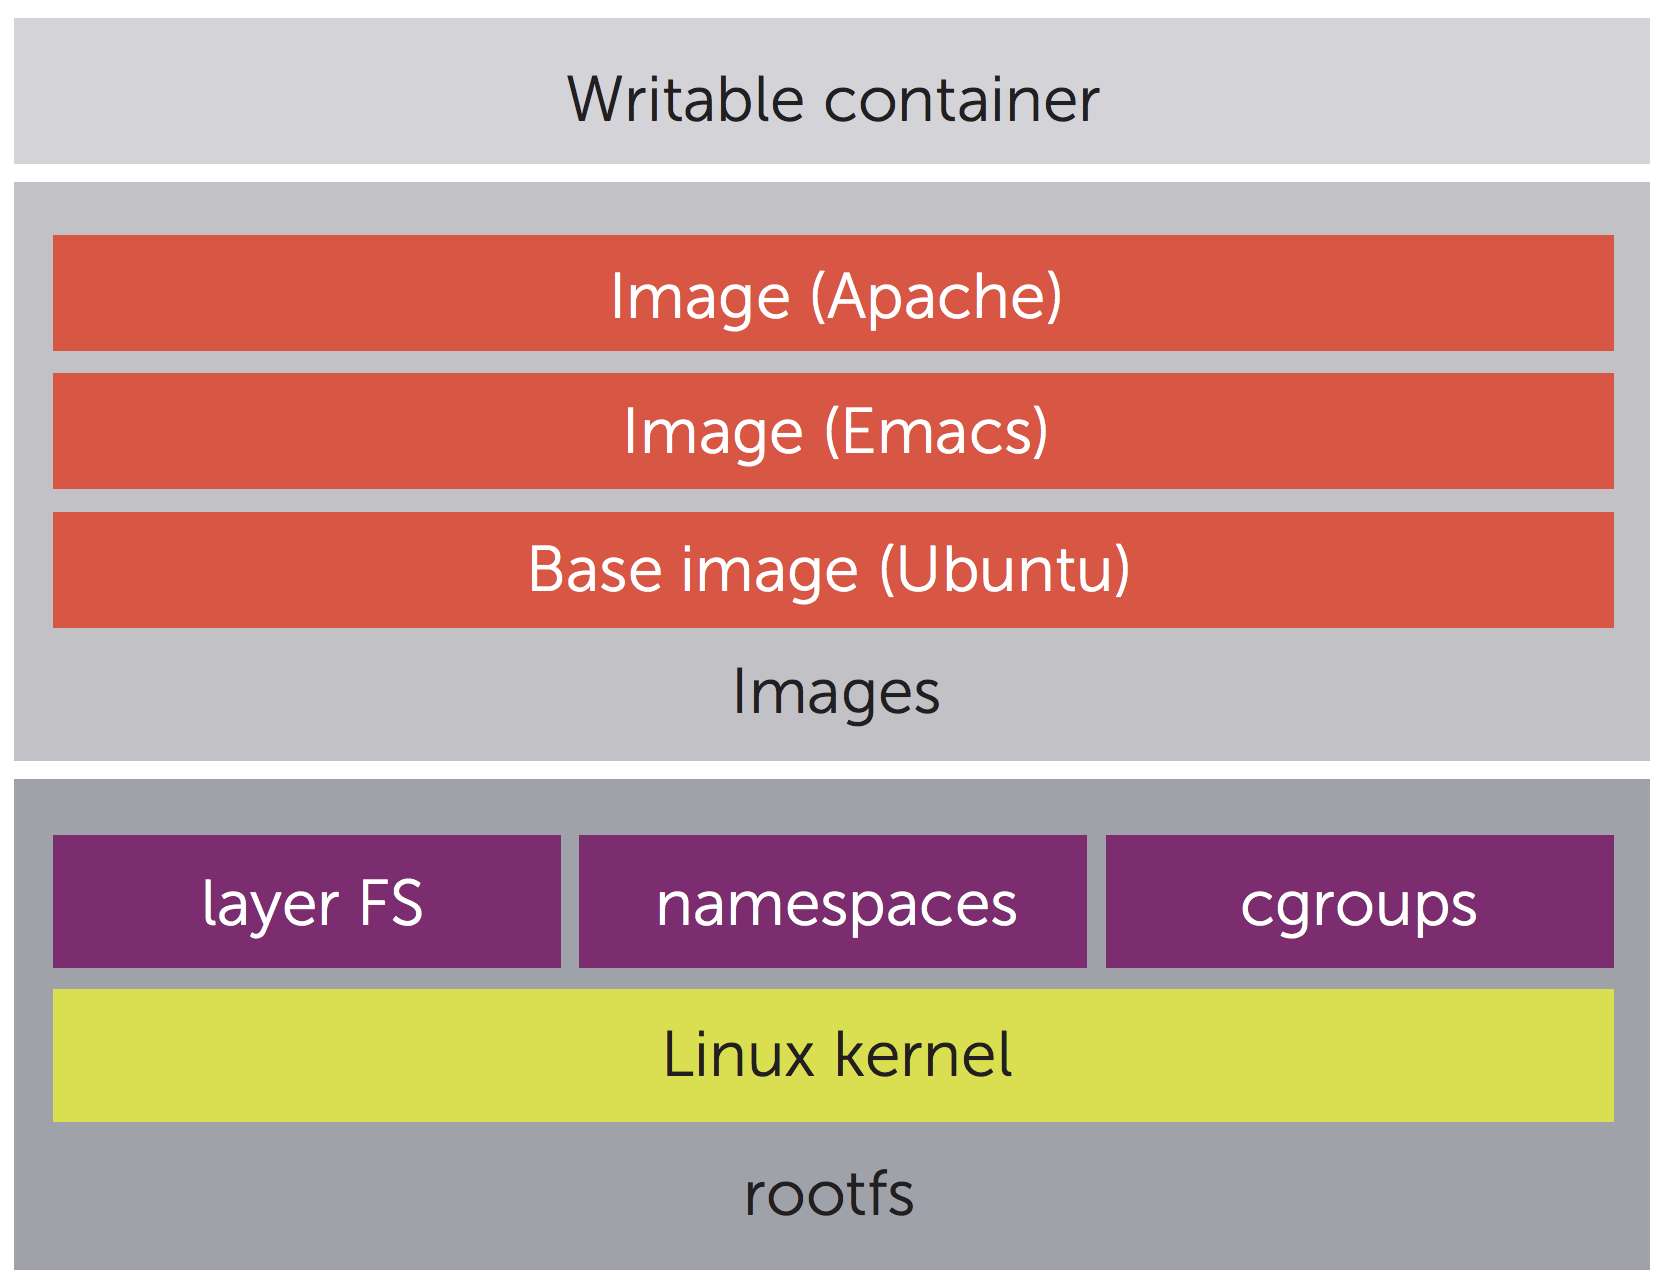
\includegraphics[width=0.5\textwidth]{chapter-background/docker-layers.png}
\end{figure}

\section{Container Orchestration}
Container technologies such as Docker offer advanced features to use containers in production. These solutions often offer deployment of applications limited to single machines. However, applications offered by  SaaS providers may include multiple different containers working together running on a cluster of nodes. Container orchestration (CO) systems allow deployment and management of containers at scale. Popular orchestration engines are Kubernetes, Docker Swarm and Mesos Marathon.
\subsection{Key capabilities of a container orchestration platform}
The task of a container orchestration (CO) platform is not limited to the initial deployment but the entire life-cycle of multiple containers. The goal of CO is to simplify cluster management while ensuring fault tolerance, availability, scalability and reliability. Allowing users to benefit from the complete potential of containers. In order to meet this goal, CO platform must at least offer the following key capabilities.~\cite{khan2017key}
\paragraph{Cluster state management and scheduling}
A cluster can be composed out of multiple virtualized or physical instances. Running containers on top of these instances and recover from failures requires a stable cluster. State management encapsulates various tasks such as flexible scheduling, re-partitioning of resources and data and propagating of dependent system changes.~\cite{khan2017key} 
\paragraph{High availability and fault tolerance}
A container orchestration platform must ensure high availability and fault tolerance in order to be useful for application developers. Most platforms therefor employ design principles of reliability engineering e.g., single point of failure elimination, failure detection or load balancing.~\cite{khan2017key}
\paragraph{Security}
Containers executing on top of the platform essentially form untrusted entities, with potentially malicious intentions, a high security standard is required. The standard should include: container images sanity check policies, access control for both containers and users, and techniques to minimize the container attack surface.~\cite{khan2017key}  
\paragraph{Simplified networking}
Containers must be able to communicate across nodes in  an efficient and secure manner. This requires the mapping of allocated host ports to containers. The overhead corresponding to this mapping intensifies at scale. The CO platform should thus provide a flexible, secure and scalable solution for networking.~\cite{khan2017key}
\paragraph{Service discovery}
The large number of services present in a cluster need to be able to communicate with each other. In traditional clusters services were handled as pets (i.e, having static names, IP addresses), however, in dynamic environments such as container orchestration platforms, they are regarded as cattle. The CO platform must provide mechanisms for addressing/labeling/grouping and service discovery.~\cite{khan2017key} 
\paragraph{Monitoring and governance}
The container orchestration platform needs to support traditional monitoring techniques such as logging, resource usage and network trace-routes. Monitoring must be possible at both the level of the underlying infrastructure and the containers themselves.~\cite{khan2017key}
\paragraph{Integrating for continuous integration and delivery}
Software development teams should be able to integrate the CO platform within their employed continuous integration and delivery (CI/CD) pipeline. The CO platform should contain mechanisms for rolling updates, rollbacks, etc.~\cite{khan2017key}


\subsection{Kubernetes}
Kubernetes~\cite{kubernetes}, commonly referred to as K8,  is one of the most popular and adopted orchestration systems. It is an open-source project led by Google. Kubernetes is Google's solution for the growing demand of container deployments by external developers in its public business cloud and is based upon its predecessors  Borg~\cite{verma2015large} and Omega~\cite{schwarzkopf2013omega} that have been used to schedule the internal Google workload. Its main design goal is formulated as:\textit{ "to make it easy to deploy and manage complex distributed systems, while still benefiting from the improved utilization that containers enable~\cite{Burns:2016:BOK:2930840.2890784}"}.  \\\\
\noindent To achieve the above stated goal Kubernetes introduces a number of concepts for both containers and cluster resources. It implements the infrastructure as code model  by provides an abstraction layer on top of the physical infrastructure~\cite{hermanns2015current}. It allows to setup and manage container infrastructure by the configuration of these introduced concepts via a REST API or declarative YAML configuration files. Below the most relevant concepts are introduced.
\subsubsection{Kubernetes concepts}
\textbf{Pods.}  A pod is the smallest unit of deployment within Kubernetes. It is a group of one or more containers that logically belong together.   A pod and thus its containers run on the same node. They share the same network, storage and context (Linux namespaces, cgroups). A pod gets assigned a unique IP address. Pods are not self-healing meaning when an error occurs within the pod or during scheduling. It will be deleted. Due to this short life cycle using a single pod resource and its assigned IP address for applications is impractical. Kubernetes handles this by employing controllers and services.~\cite{pods}\\\\
\textbf{Deployments.}  A Deployment controller manages a pod or a ReplicaSet of pods. A ReplicaSet allows pods to be replicated across multiple nodes. A Deployment object is used to specify the desired state of pods (e.g. number of replica's). A deployment, in addition, allows for declarative updates. These updates can be used to change the number of container replicas of a ReplicaSet or to update a specific container image within the pod.  The Deployment controller changes the actual state to the desired state described by the update.~\cite{deployments}
\\\\
\textbf{Services.}  Services offer a solution for the short life cycle of pods (and their IP addresses). Services within Kubernetes offer a manner to expose a ReplicaSet of Pods via a unique name, stable IP address, network policy and ports. To determine which set of pods is targeted by a service, Kubernetes employs a Label selector. Labels are the core grouping primitive of Kubernetes and unlike names and UIDs do not offer uniqueness.\\  A Service can be exposed outside the cluster by using an external load balancer or by specifying a NodePort. When using a Nodeport each node within the cluster will expose the port and forward request into the service.~\cite{services}
\\\\
\textbf{Namespaces.}  Namespaces allow to partition resources of a physical cluster among multiple user organizations. Each namespace gets a share of the resources of the cluster, via resource quotas. Resource quotas are supported for CPU, memory and persistent volumes.~\cite{namespaces-k8}
\\\\
\textbf{Resource limits.}  Kubernetes allows the allocation of compute resources of both containers and Namespaces by the means of resource limits. These limits can be soft (limit) and hard (request) limits. A Request specifies the quantity of resource that is guaranteed to the container. A limit specifies the maximum quantity allocated to the container. When the requested resource quantities of a container are less than its limit, the container may be allocated additional resources if there are unallocated resources available.  The current supported compute resources are CPU, memory and storage within the root partition of the local node. Within a Pod it is possible to specify both request and limit for each container. When request and limits are specified, the scheduler will use them for both scheduling and eviction (when node capacity is reached) decisions.~\cite{kubresources}
\subsubsection{Kubernetes architecture}
The basic architecture of Kubernetes is illustrated in Figure~\ref{fig:kubarch}. A client-server architecture is employed in which master and node setups are deployed on different machines. Below the different components that build up the architecture are briefly explained. 
\paragraph{API Server.} The API server is responsible for the configuration and validation of API objects (pods, deployments, services,...). It offers communication on cluster state via a REST interface for both components and administrators.~\cite{kubernetes-api-server}
\paragraph{Controller manager.} The controller manager is responsible for managing several core control loops part of Kubernetes. A control loop uses the API server to observe the shared state of the cluster and attempts to move to the desired state via configuration changes.~\cite{kubernetes-controller-manager}
\paragraph{Scheduler.} The task of assigning pods to nodes is the responsibility of the scheduler component.  The scheduler attempts to do a reasonable placement based on resource and quality of service requirements (e.g., not place a pod on a node with insufficient resources). It is  possible for users to control the placement of pods via NodeSelector tags or affinity and anti-affinity constraints in the configuration file.~\cite{kubernetes-pods-to-nodes,kubernetes-scheduler}
\\\\In addition it is possible to assign Quality of Service (QoS) classes to pods. These are used by Kubernetes in the decision process about scheduling and eviction of pods. Currently, Kubernetes supports three types of classes: guaranteed, burstable and best-effort. In decreasing order of priority (i.e., most likely to be killed in the case of resource shortages). The QoS classes are assigned to pods based on the presence of request and limit specifications of resources in their configuration files.~\cite{kubernetes-qos}


\paragraph{Kubelet.} The kubelet component is an agent running on each node. It is responsible for running and maintaining pods on its residing node. The set of maintained pods is described in the form of PodSpecs (mainly received via the API-server).~\cite{kubernetes-kubelet}
\paragraph{Kube-proxy.} The kube-proxy daemon provides a simple network proxy for the services on each node. It enables forwarding of requests to the correct containers and can provide primitive load balancing.~\cite{kubernetes-kubeproxy}
\begin{figure}[H]
\caption{Kubernetes architecture}
\centering
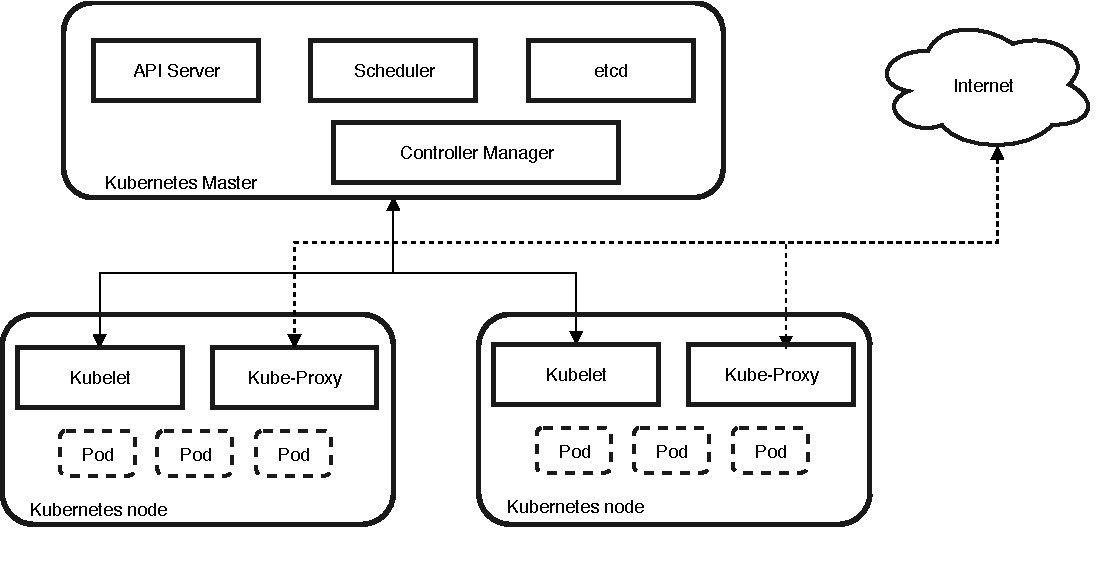
\includegraphics[width=0.8\textwidth]{chapter-background/kubernetes-architecture-diagram.pdf}
\label{fig:kubarch}
\end{figure}
 
 
 
 
 
 
 
 
 
 \section{Performance evaluation}
As discussed in previous sections, SaaS providers employ multi-tenancy to improve  cost efficiency and offer several performance guarantees to their customers in the form of SLOs. An unavoidable consequence of multi-tenancy is the need to support a growing number of users in a single system. Providers need to have a clear insight into the \textit{scalability} of their systems. However, scalability is a difficult thing to define, let alone quantify. Citing the words of  Dr. Neil J. Gunther:  \textit{"if you can't quantify it, you can't guarantee it"}.~\cite{perfdynamics}

\subsection{The Universal Scalability Law}
\label{section-USL}
Dr. Neil J. Gunther provides a formal definition of scalability: \textit{"scalability can be defined as a mathematical function, a relationship between independent and dependent variables (input and output)"~\cite{perfdynamics}}. The Universal Scalability Law (USL) by Dr. Neil J. Gunther is presented in Equation~\ref{USL}. It computes the relative capacity $C(N)$ at a load of $N$ users. Relative capacity is the normalized throughput.
\begin{equation}
\label{USL}
C(N) = \frac{\gamma~N}{1 + \alpha~(N-1) + \beta~N~(N-1)}
\end{equation}

The Universal Scalability Law incorporates factors that contribute to the sublinearly scalability of most systems. Namely, \textbf{concurrency} ($\gamma$), \textbf{contention} ($\alpha$) and \textbf{coherency} ($\beta$) as explained below. Their impact is visualized in Figure~\ref{fig:usl-impact}.

\begin{itemize}
    \item \textbf{Concurrency}($\gamma$): $\gamma$ defines the slope if the system was linearly scaling i.e., $C(N) = \gamma N$. It has been referred to as the \textit{coefficient of performance} by~\cite{schwarz2015practical}.
    \item \textbf{Contention} ($ \alpha $) : When scaling most systems parallelism while be limited at some point by contention (i.e., waiting or queuing for shared resources). The maximum speedup by parallelism is limited by the serialized portion ($\alpha$) of the work~\cite{schwarz2015practical}. 
    \item \textbf{Coherency} ($\beta$): created by crosstalk between components. Because crosstalk is possible between each pair of components in the system, the penalty grows quadratic $N(N-1)$.~\cite{schwarz2015practical}
    
\end{itemize}

\begin{figure}
    \centering
    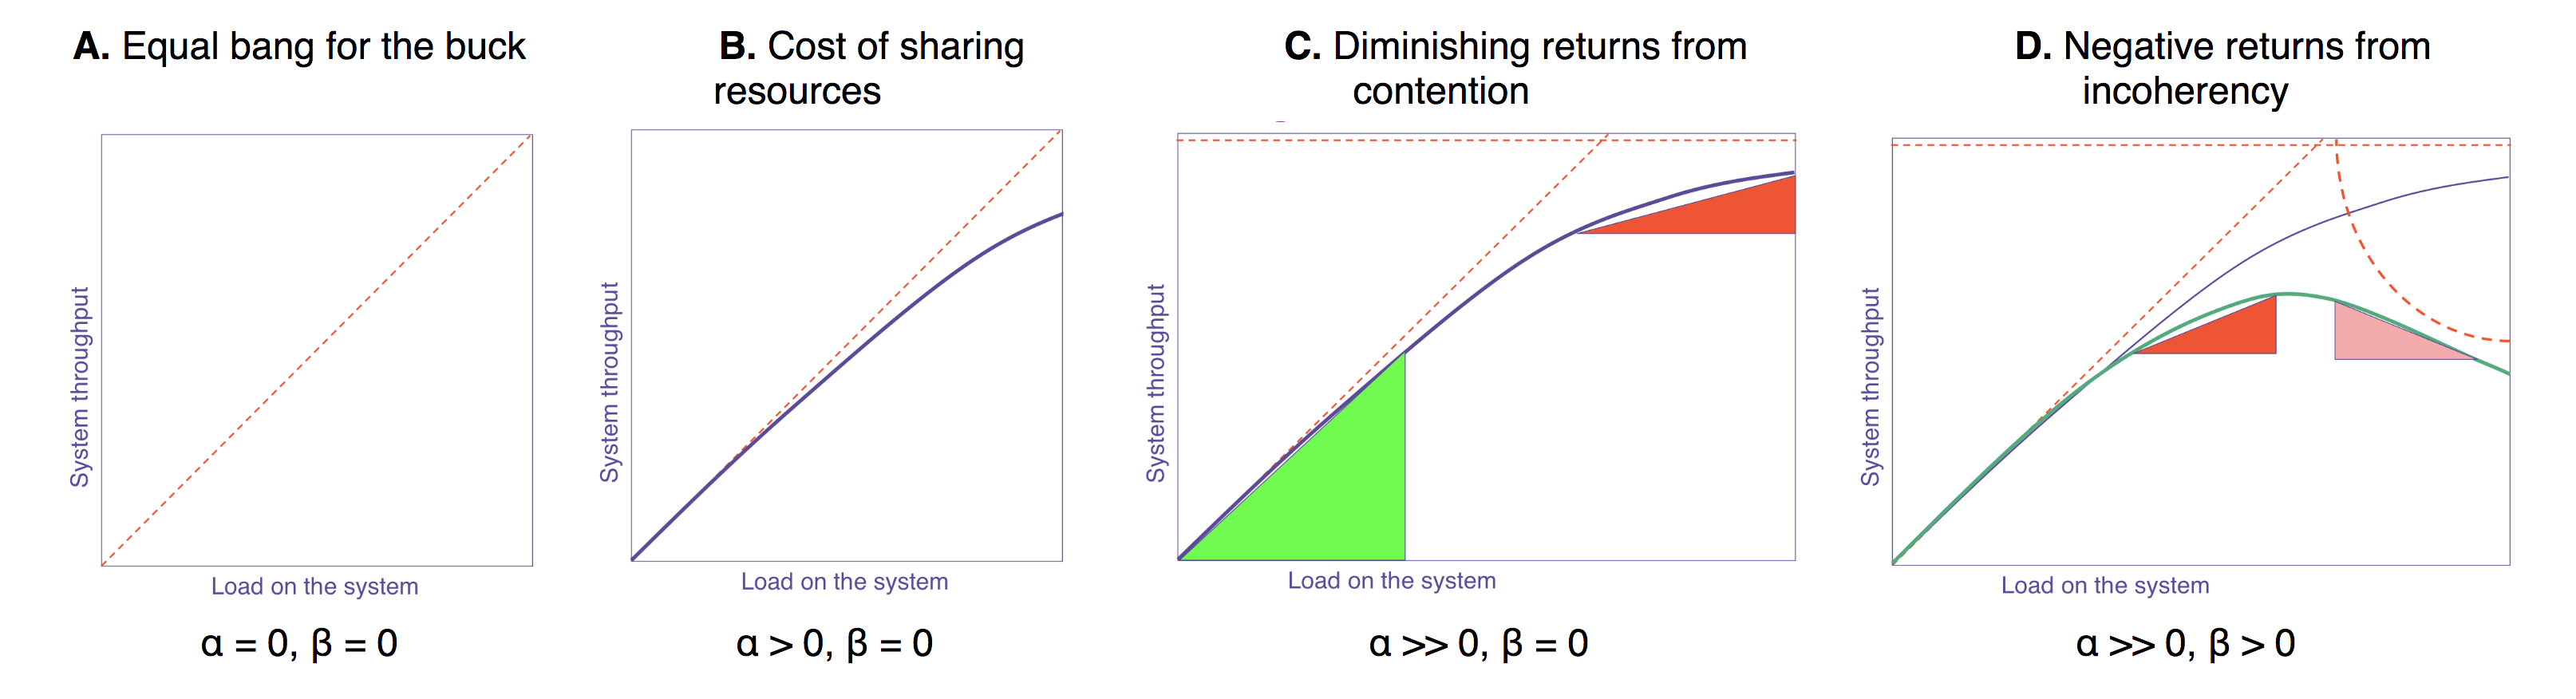
\includegraphics[width=1.1\textwidth]{chapter-evaluation/usl-impact}
    \caption{The impact of different USL coefficients on scalability.~\cite{perfdynamics}}
    \label{fig:usl-impact}
\end{figure}

\subsubsection{USL in practice}
USL can provide insights into a system's scalability pains via  values of the concurrency, contention and coherency coefficients. These can be obtained by collecting a dataset of measurements of the system, system load $N$ and corresponding throughput, and using a statistical technique such as nonlinear least square regression which fits the USL to the dataset.~\cite{schwarz2015practical,heyman2014scalability}

\subsection{Little's law}
\label{sec:little}
The Universal Law of Scalability serves as an alternative for the often less intuitive queuing models frequently used for modeling scalability. It omits the need to know the service time for every queue in the performance model in order to predict the response time or latency~\cite{perfdynamics}. Nevertheless, queuing theorem and its lemmas such as Little's Law can provide useful insights into performance modeling.\\\\
John D.C Little's Law~\cite{little2008little} states the following for stable systems: 
\begin{displayquote}
\textit{"The average number of items in a queuing system equals the average rate at which items arrive multiplied by the average time that an item spends in the system.\cite{little2008little}"}
\end{displayquote}
\begin{equation}
\label{littleslaw}
L = \lambda~W
\end{equation}
\begin{equation}
\label{llsys}
N = X~Rt
\end{equation}
Equation~\ref{littleslaw} shows Little's law, below its terms and its applicability to web services (Equation~\ref{llsys}) are explained:
\begin{itemize}
    \item \textbf{$L$}:  Average number of items in the system. For a web service this is represented by the average number of concurrent users in the system $N$.
    \item \textbf{$\lambda$}: Long-term average arrival rate of items in the system per time unit. Little's law assumes a stable system for which the arrival rate and exit rate are identical. In a web service this is represented by the throughput $X$.
    \item \textbf{$W$}: Average waiting time of an item in the system, queuing time and service time combined. This is represented by the response time $Rt$ or latency of a request in a web service. When dealing with a system involving think time (e.g., after the response from a web service, a user needs time to think about his/her next request), $(Rt + Zt)$ is used. 
\end{itemize}

\subsubsection{Workload generator validation}
Developers employ software tools (JMeter~\cite{jmeter}, Locust~\cite{locust}, etc.)  to simulate a workload and test the performance of a system. A workload is a set of actions that represent the behavior of a client in the system. It is part of the test plan stating the number of concurrent users $N$ executing the workload for a specified period of time.\\\\
The results of a performance test are typically expressed in throughput $X$ and response time $Rt$. Using Little's law it is possible to validate these results. For example, a test plan of 1000 concurrent users $N$ results in a throughput of 50 requests per second and an average response time of 15 seconds. Following Little's law, a concurrence of only 750 users was reached, instead of the specified 1000. Little's law can thus be used to check if a workload generator works as specified.\\\\
Alternatively, if the average throughput and response time for a production system are known, Little's law can be used to correctly draw up a test plan.

\subsubsection{Response time or latency?}
Performance can either be measured in throughput or latency, both are correct but offer a different point of view. System performance is typically expressed in throughput: "The system can handle a million operations per second". However, users care more about their personal experience with a system which is influenced by the average latency of their request.~\cite{schwarz2015practical} \\\\
Figure~\ref{fig:ls_vs_tp} shows the relation between the average latency and throughput of a database under increasing load $N$. In this case, latency is kept stable by increasing the throughput with the increasing load up to a certain point.  A bottleneck caps the throughput of the systems and by Little's law for an increasing load and constant throughput, the latency must increase.~\cite{latvsthrough} \\\\
However in other systems, as discussed in Section~\ref{section-USL}, an increasing load might induce a diminishing result on the system's throughput. Following Little's law a decreasing throughput results in a higher latency under the same load. \\\\
Thus, for stable systems by Little's law,  the USL can be reformulated in terms of latency instead of throughput. Equation~\ref{USL-2} shows this reformulation.~\cite{schwarz2015practical}
\begin{equation}
\label{USL-2}
Latency(N) = \frac{1 + \alpha~(N-1) + \beta~N~(N-1)}{\gamma}
\end{equation}


\begin{figure}[H]
    \centering
    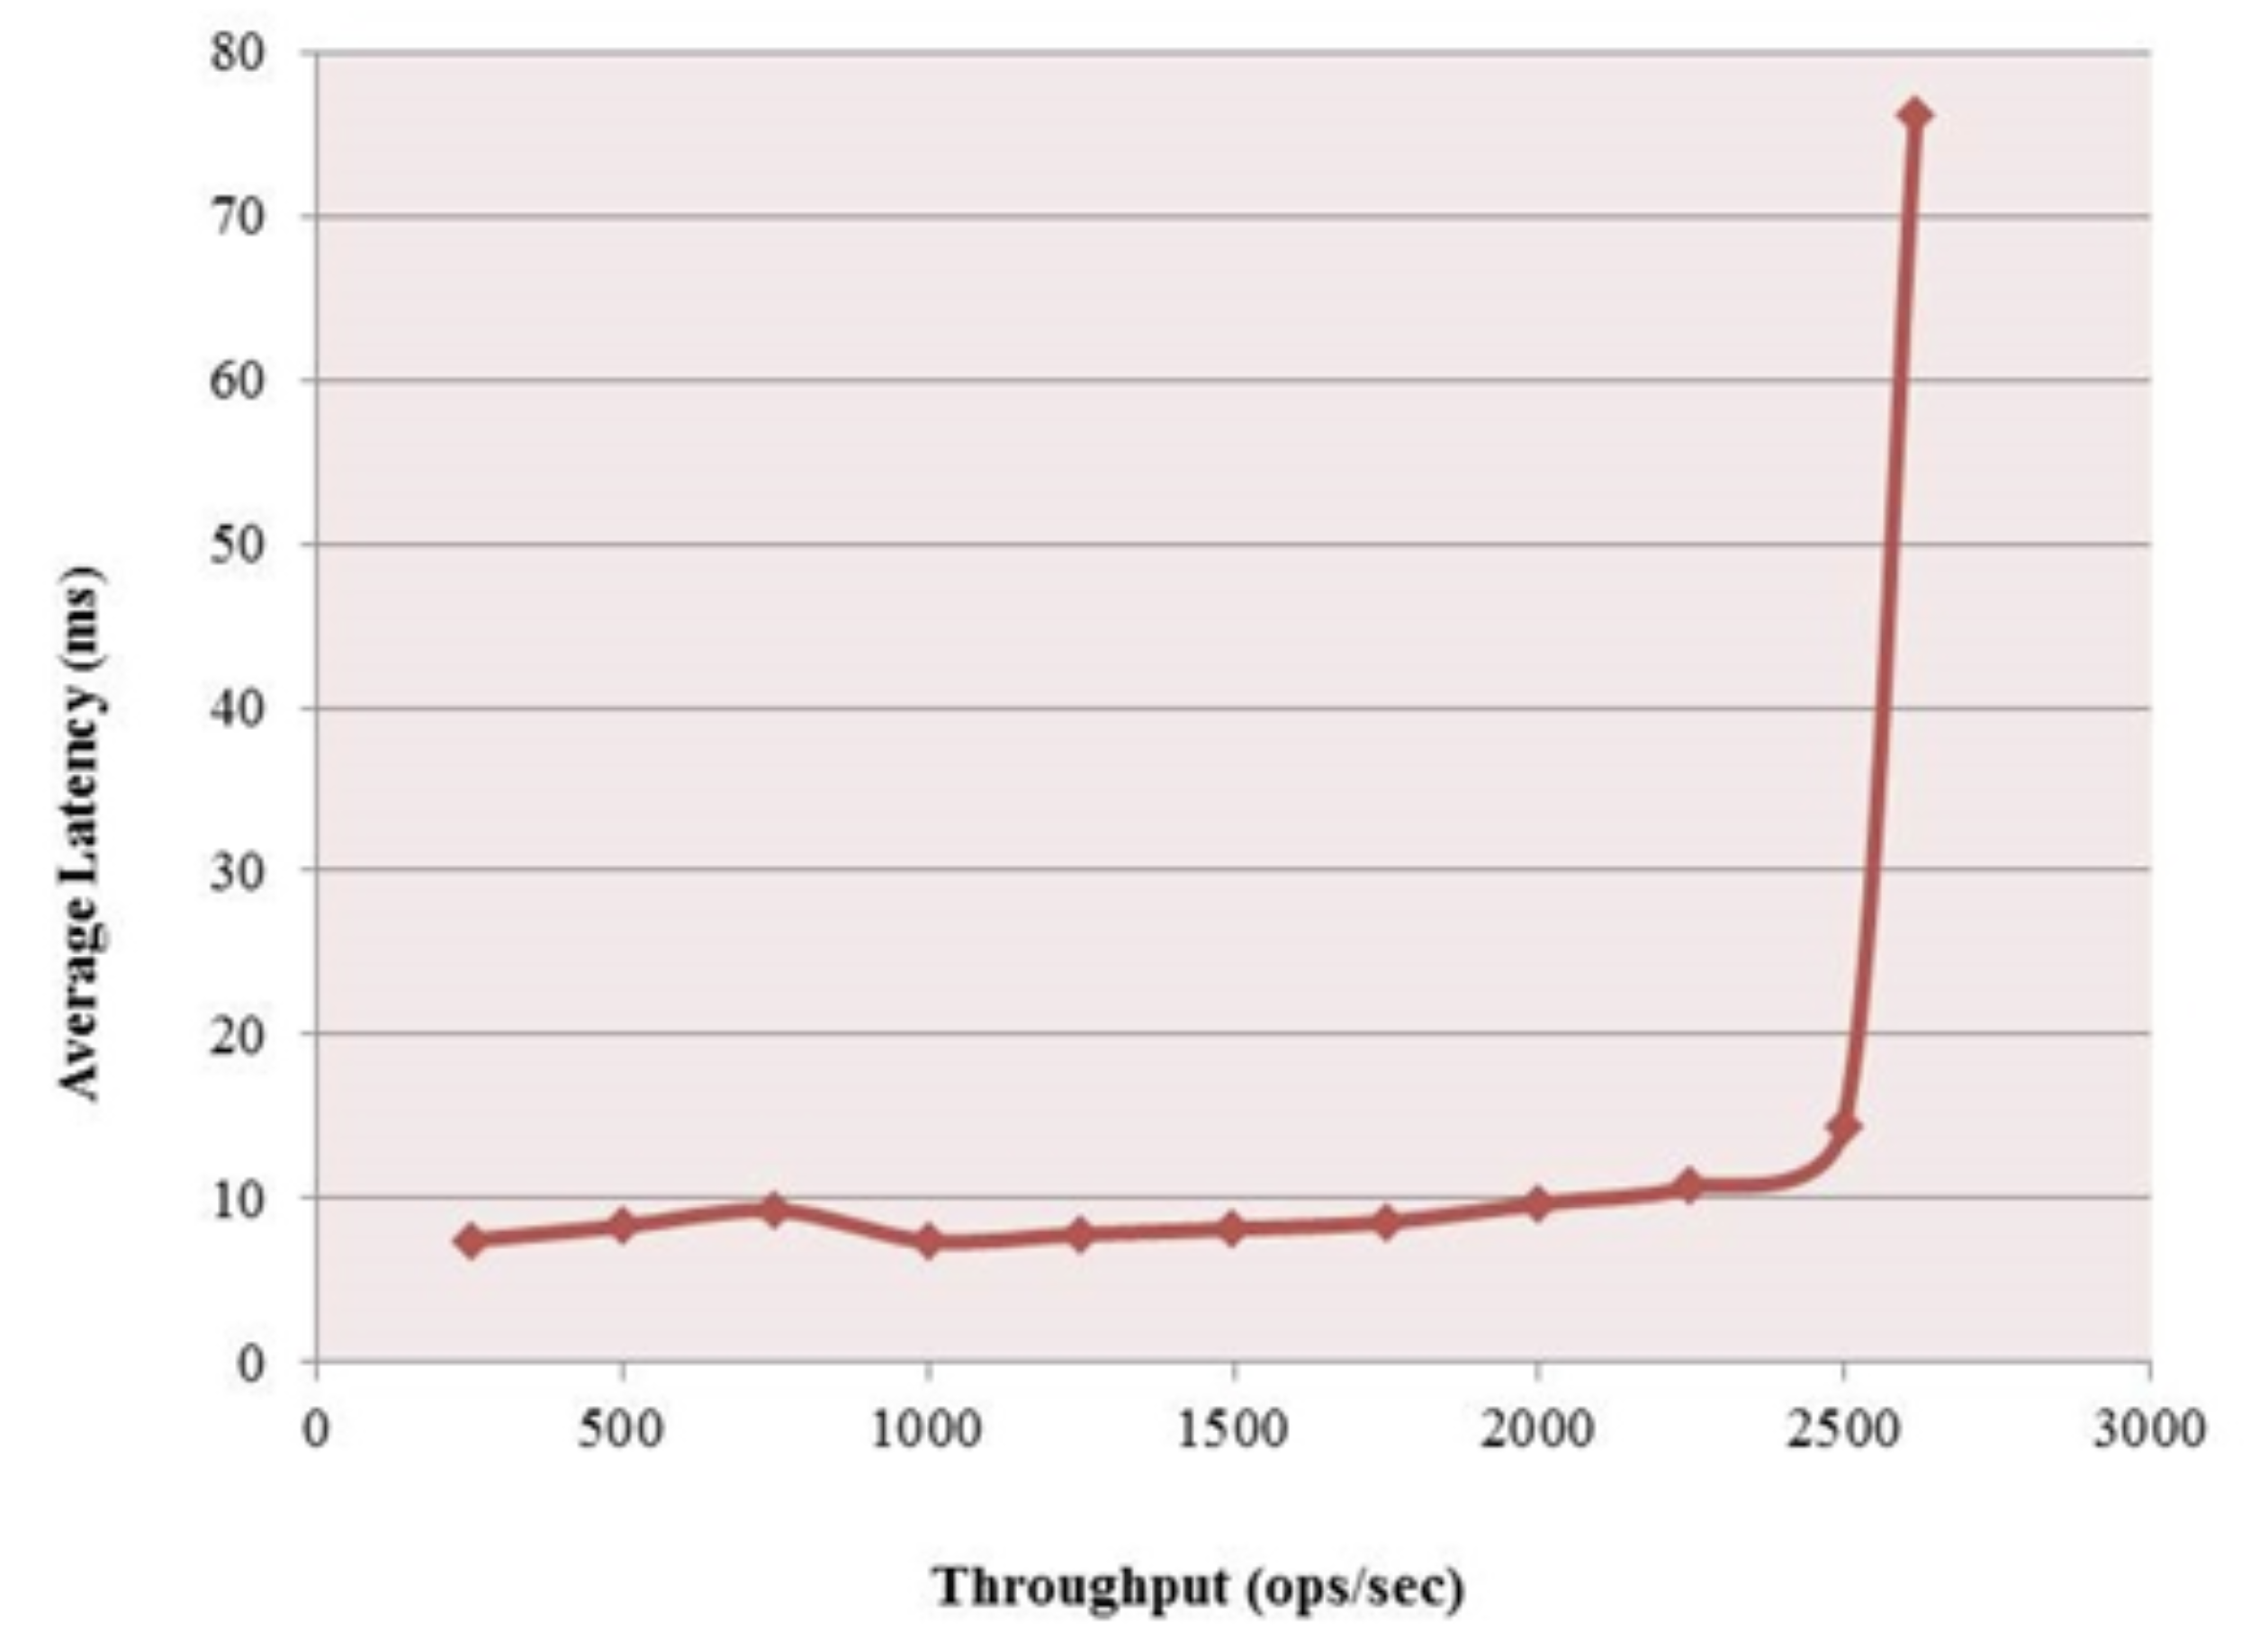
\includegraphics[width=0.8\textwidth]{chapter-evaluation/ls_vs_th}
    \caption{Relation average latency vs. throughput for database benchmark with increasing load.~\cite{latvsthrough}}
    \label{fig:ls_vs_tp}
\end{figure}
\chapter{Background}
\label{ch:background}
This chapter discusses relevant background material for the thesis. The concepts, explored in this chapter, further clarify the relevance of the thesis and serve as building blocks for the remaining chapters. Starting from the adoption of the cloud computing paradigm, the chapter elaborates on how concepts such as multi-tenancy and virtualization via containerization push the limits of efficient resource utilization. Next, an in-depth overview of the open-source container orchestration platform Kubernetes is provided. Lastly, insights are provided into the universal scalability law and the applicability of Little's law for performance testing.
\section{Cloud computing}
Companies try to minimize the total cost of ownership by moving to cloud computing or utility computing. The cloud computing paradigm enables on-demand access to a shared pool of configurable compute resources (software applications, system software and hardware infrastructure)~\cite{WalravenStefan2015PPmf}. A service provider can provision the required resources from the cloud with minimal effort.  Within this paradigm, services are offered in real time over the internet in three different models~\cite{MellPeter2010TNDo,rimal2009taxonomy}. 
\begin{itemize}
\item \textit{Infrastructure as a Service (IaaS)} in which access is offered to virtual machines, network, data storage and other fundamental computing resources. The customer is able to deploy arbitrary software using these resources.\\\\
Examples: Digital Ocean, Microsoft Azure and Amazon Elastic Compute Cloud (EC2).
\item \textit{Platform as a service (PaaS)} offers customers a platform enabling easy and efficient deployment of applications (at scale) while abstracting the complexity of managing the underlying infrastructure. PaaS allows customers to solely focus on the development of their application.\\\\
Examples: Google app engine, Microsoft Azure and Heroku.
\item \textit{Software as a service (SaaS) } allows customers to make use of a specific application developed by a SaaS provider. Compared to the traditional use of software, the management and deployment is the task of the SaaS provider. In this strategy, common resources and a single instance of both the application and underlying database are used to support multiple customers simultaneously. \\\\
Examples: Google apps and Salesforce.
\end{itemize}

\section{Multi-tenancy}
\label{multi-tenancy}
The software as a service (SaaS) model offers applications to customers as an on-demand service. Providers of these applications try to leverage economies of scale by employing a multi-tenancy architectural design principle. The goal of multi-tenancy is to minimize the total cost of ownership for the provider by maximizing the sharing of resources among multiple customers organizations, referred to as tenants.~\cite{Walraven2015b} 
\subsection{Service Level Agreements}
By moving their core business functions to an entrusted cloud provider, cloud customers give up control of the underlying compute resources. It is vital for these tenants to obtain certain guarantees on the service delivered by the provider. 
A Service Level Agreement (SLA) is a formal contract between the SaaS provider and the tenant specifying both properties of the provided service and the expected behavior of the tenant. An SLA typically also contains a set of Service Level Objectives (SLOs). An SLO is a measurable characteristic of the service. An SLO is typically related to performance constraints (latency, throughput and deadlines) or availability (uptime percentage) of the service. Within the specification of an SLA a trade-off must often be made between expressiveness and usability. The SLA must cover all the expectations of a customer while remaining simple to weight, verify, evaluated and enforce~\cite{dillon2010cloud}.  Some typical examples of SLOs are shown below: 
\begin{itemize}
\item The application has a monthly uptime percentage of 99.95\%.
\item If the arrival rate of the tenant workload < X requests/s then a throughput T is guaranteed.
\end{itemize}
\subsection{Challenges}
While the goal of multi-tenancy is promising, sharing a cluster of dynamically provisioned nodes between multiple tenants imposes a number of challenges and requirements~\cite{TruyenEddy2016Taca}. 
\begin{itemize}
\item Performance isolation: the activities of one tenant should not be able to influence the service level delivered to other tenants. This requirement should be achieved during normal system load and when an aggressive tenant violates the terms of the SLA. 
\item QoS differentiation: the performance guarantees specified by an SLA can be individually customized for each tenant. A SaaS provider should be able to offer different subscriptions.
\item Flexible resource allocation for improved server consolidation: a SaaS provider employs a multi-tenant architecture to achieve a lower operational cost. This is partially achieved by planning the required node capacity based on the actual resource usage of tenants instead of the theoretical required capacity.  This can be further aided by the use of request schedulers allowing to distinguish between normal, passive and aggressive tenants. 
\end{itemize}
\subsection{Strategies}
To achieve multi-tenancy different strategies, each offering different trade-offs concerning operational costs and upfront application engineering costs, can be employed by the SaaS-provider~\cite{WalravenS.2011Amlf}. The strategies are illustrated in Figure~\ref{muti-tenant-strategies}.
\begin{itemize}
\item Multi-tenancy can be achieved at the level of the \textit{operating system}. In this strategy, a virtualization technology can be used to partition compute resources among multiple virtual machines. Each tenant is assigned an application instance running on a dedicated virtual machine. This approach offers both a higher level of performance isolation and lower upfront engineering costs but suffers from an inefficient utilization of resources.
\item In \textit{middleware-level multi-tenancy} a middleware platform is used to enable sharing compute resources between multiple tenants at the level of the operating system. An application instance is deployed on top of the middleware platform for each tenant. By not replicating the operating system for each tenant a higher level of cost efficiency can be achieved but an increased complexity in managing resources and  performance isolation is introduced. By tackling these problems at the level of the middleware a part of the engineering complexity is shifted to this level.
\item The most efficient resource utilization can be achieved by sharing application instances between multiple tenants. In \textit{Application-level} multi-tenancy achieving performance isolation is done by the application itself thereby increasing the engineering complexity and costs.
\end{itemize}


\begin{figure}[H]

\caption{Different strategies to achieve multi-tenancy~\cite{WalravenS.2011Amlf}.\label{muti-tenant-strategies} }
\centering
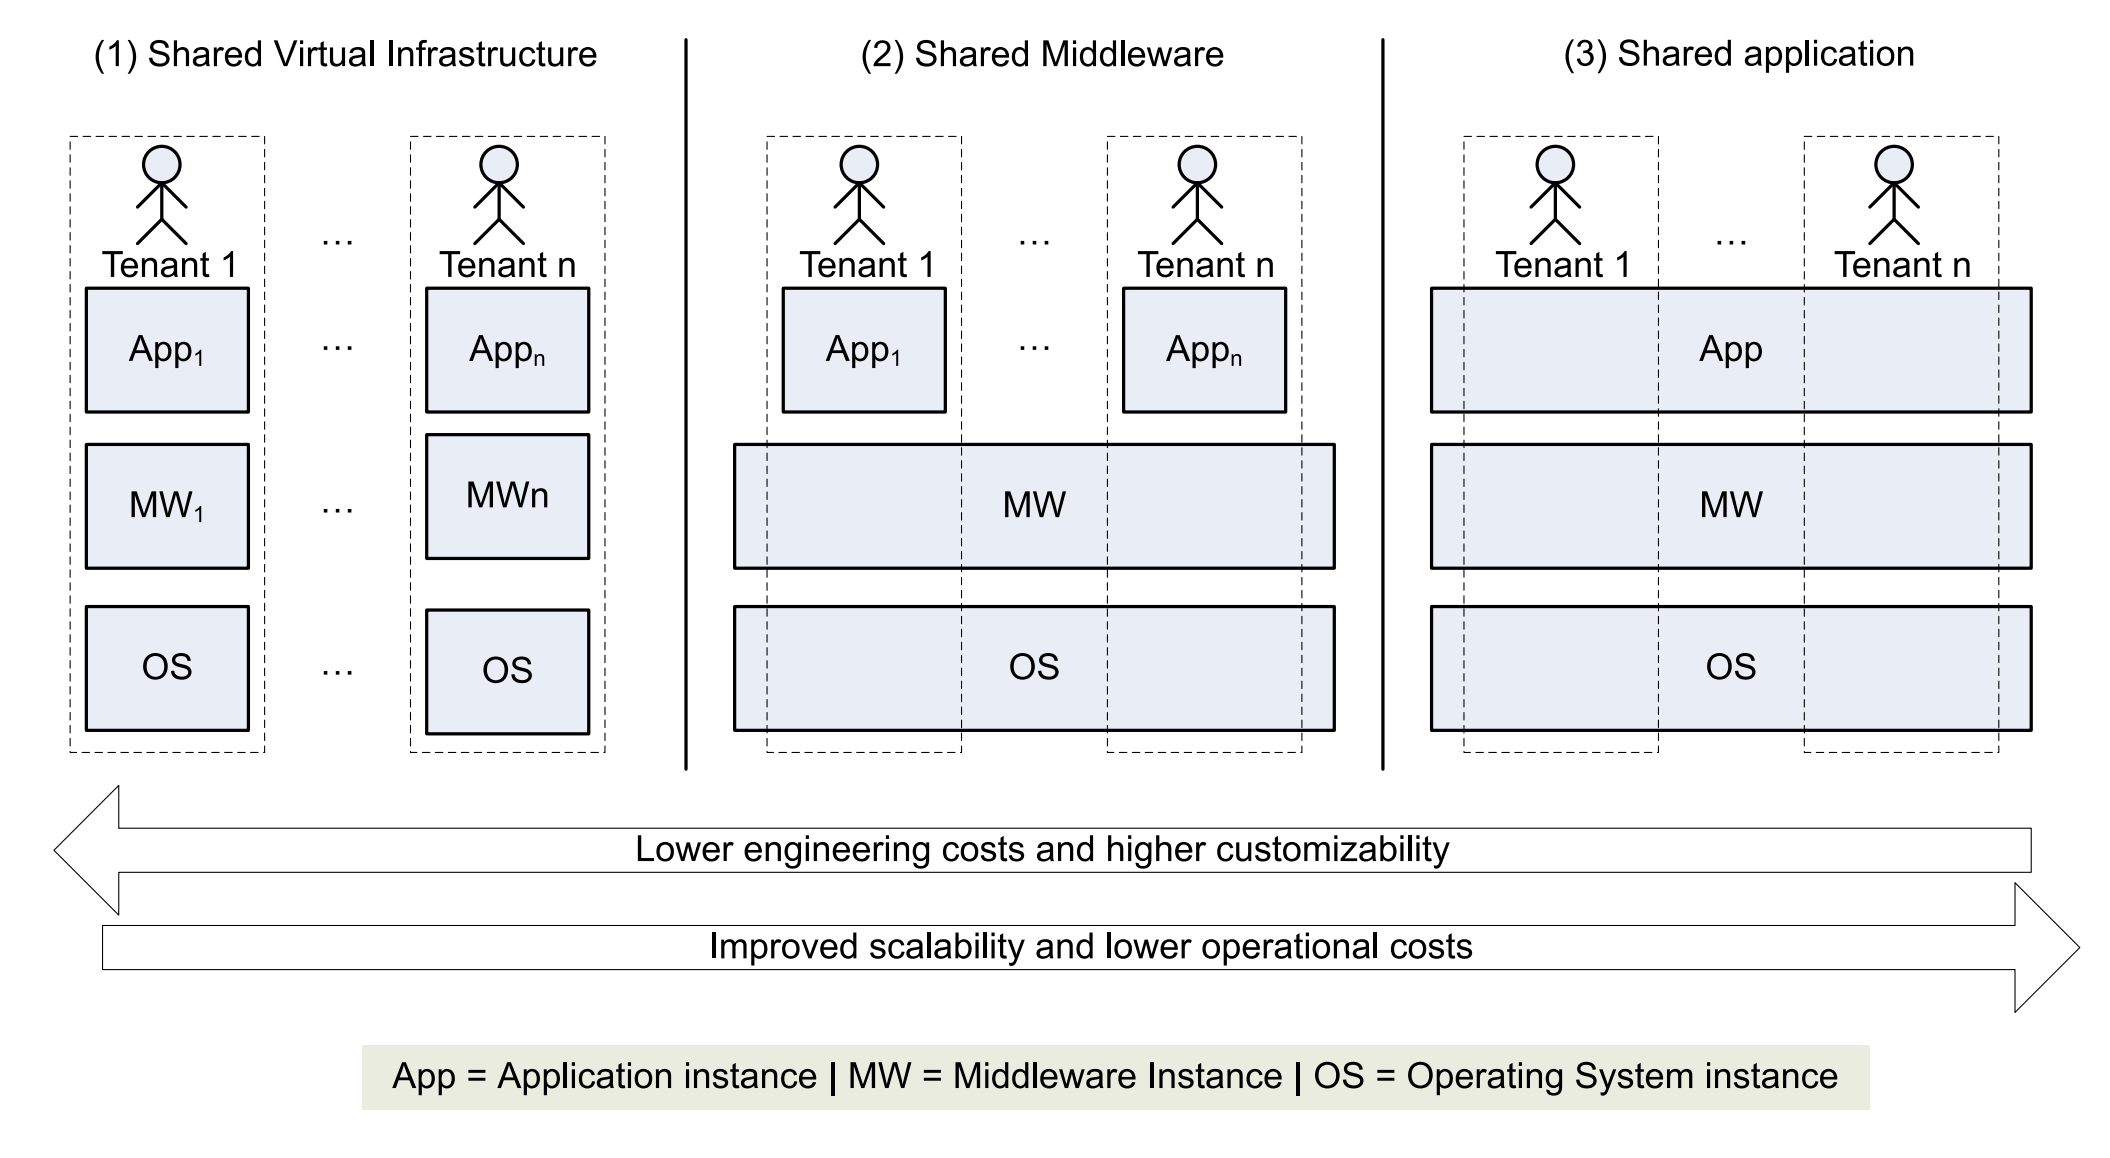
\includegraphics[width=0.65\textwidth]{chapter-background/muti-tenant-strategies.png}
\end{figure}


\section{Containerization}
Cloud providers rely on virtualization technology for the achievement of large-scale resource scaling. For more than a decade, virtual machines (VMs) have been the backbone of a provider's infrastructure offering hardware independence, availability, isolation and security~\cite{xavier2013performance}. More recently, containers a more lightweight virtualization technology have made advances in their multi-tenant capabilities and have seen an increase in adoption by providers~\cite{pahl2015containerization}. Both are discussed in this section.
\subsection{Virtualization technology}
In cloud environments, virtualization technology is used for flexible and dynamic allocation of physical resources to virtualized applications and to achieve multi-tenancy by sharing a physical server among multiple applications. In data centers virtualization is commonly used at the \textit{hardware level} and \textit{operating system level} to deploy and manage virtual machines and applications at scale~\cite{SharmaPrateek2016CaVM}. \\\\
Hardware level virtualization uses a hypervisor on a server to create virtual machines. Each virtual machine provides an abstraction of a physical machine and runs an independent operating system with applications. The hypervisor is responsible for resource allocation and performance isolation.\\\\
Operating system level virtualization allows resources to be shared at the level of the OS. Virtual machines running at the OS level are referred to as containers. Isolation, abstraction and resource allocation of containers is performed by the OS kernel of the host OS. By sharing the OS kernel among multiple containers, containers are regarded as a more lightweight virtualization technology. Containers only contain the application and its dependencies.\\\\
Linux containers (LXC)~\cite{lxc} employ different mechanisms of the Linux kernel to achieve resource isolation, namely control groups and namespaces.
\begin{itemize}
    \item \textbf{Cgroups}~\cite{cgroups} allow for fine-grained control of the allocation of system resources (CPU time, system memory, network bandwidth) among processes and process groups. For example, it is possible to limit or prioritize memory, CPU or I/O usage of different containers. 
    \item \textbf{Namespaces}~\cite{namespaces} allow for isolation of kernel resources among processes. A namespace makes a resource appear to be private and isolated for the container. The Linux kernel provides the following namespaces:  process ids, inter-process communication (IPC) mechanisms, network stack and mount points.
\end{itemize}
Linux containers (LXC) offers a lightweight implementation which performs at native speed and provides good isolation. However, while sharing a kernel between containers minimizes overhead, there are limitations in terms of the security environment.~\cite{dua2014virtualization}
\\\\
\noindent By offering virtualization at different levels, containers and VMs offer different trade-offs concerning performance isolation and performance. Research~\cite{SharmaPrateek2016CaVM} concludes that while containers offer closer to bare metal performance compared to VM, they offer worse performance isolation in multi-tenant environments. In addition, containers offer soft resource limits compared to the hard resource limits of virtual machines which allow for better server consolidation in over-commitment scenarios.  
\begin{figure}[h]
\caption{Container vs virtual machine.~\cite{container-vs-vms}}
\centering
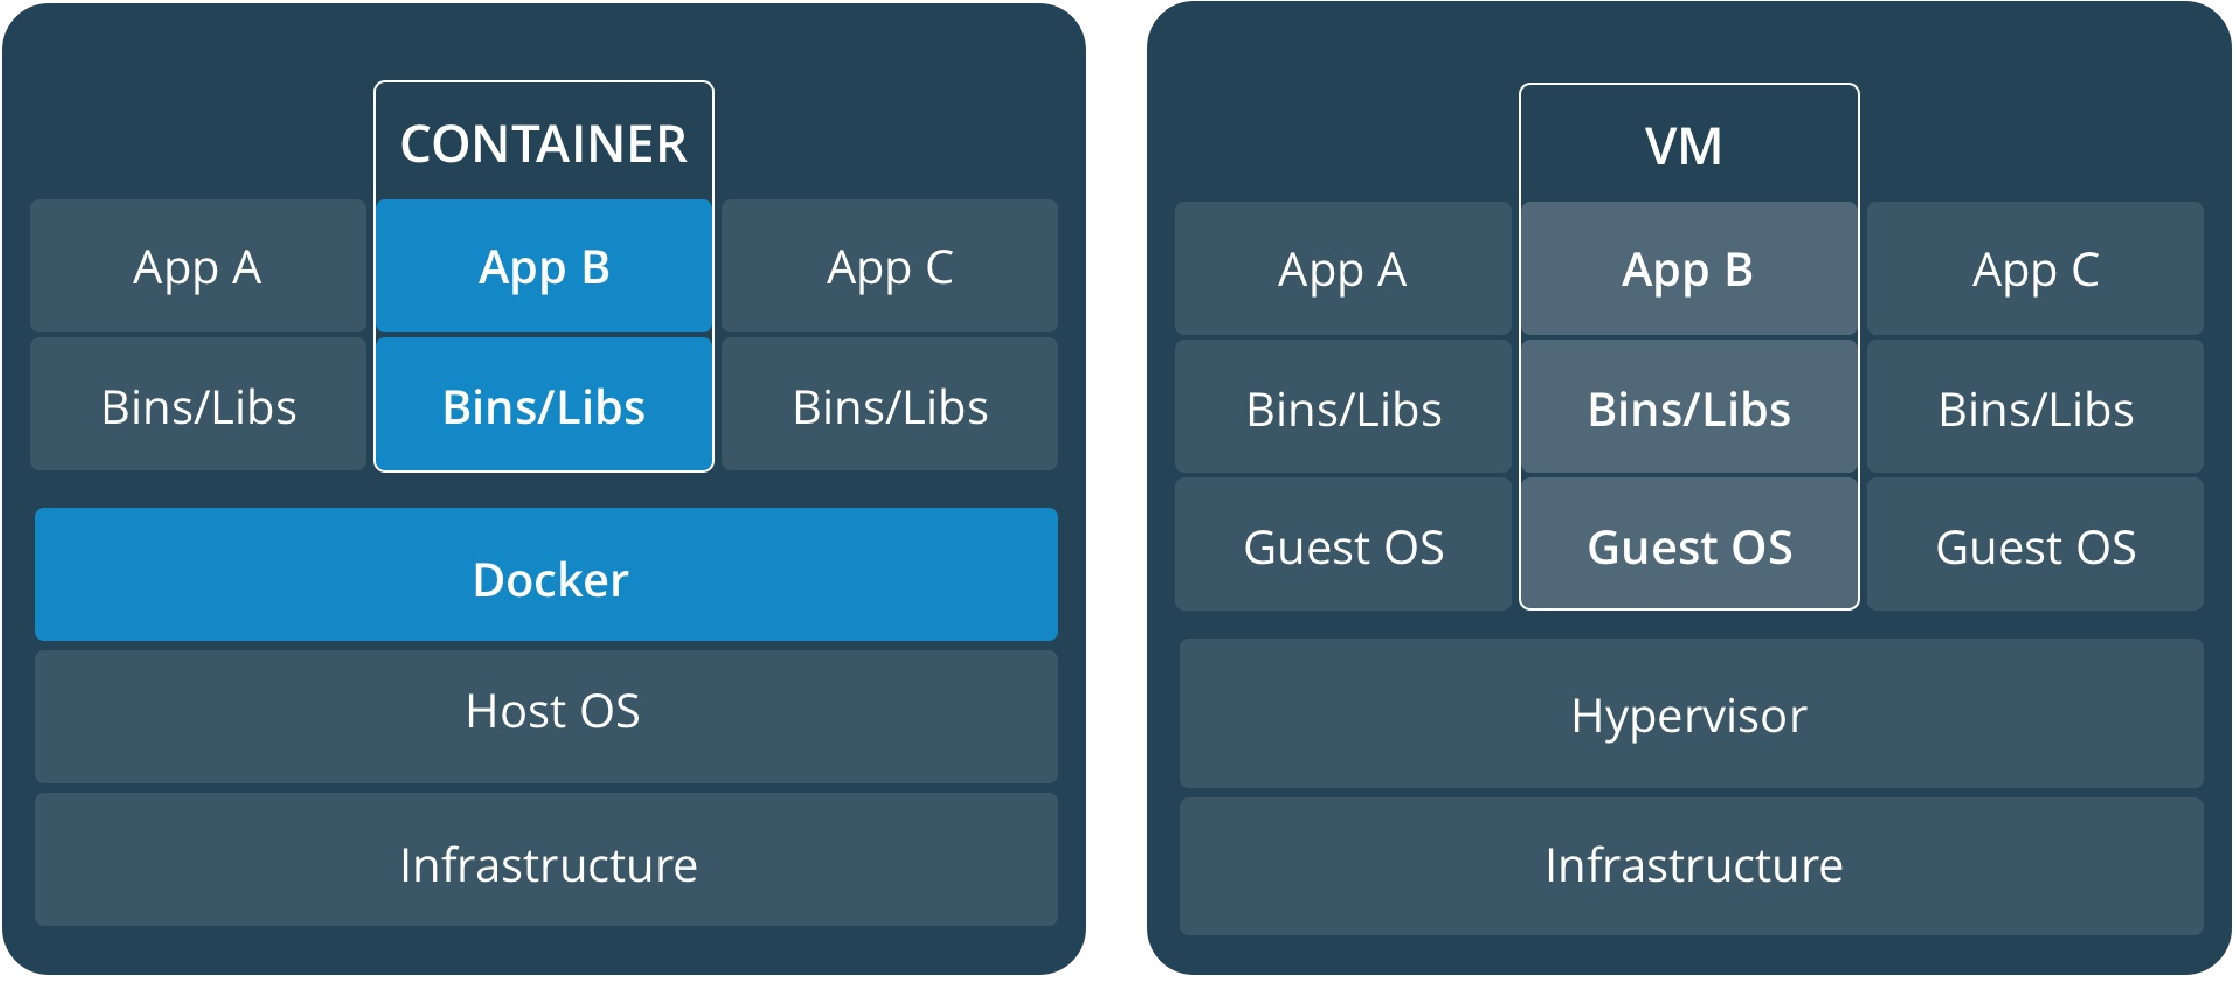
\includegraphics[width=0.8\textwidth]{chapter-background/containervsvm.pdf}
\end{figure}
\subsubsection{Docker}
Recently, thanks to Docker~\cite{dockersite}, containers have gained popularity and have been adopted into the software development process. However, Docker is not a new container technology, at its core it employs the kernel-level mechanisms of Linux containers (LXC), for which it defines a unified API~\cite{merkel2014docker}. In addition, the open-source Docker project offers a commandline-interface and daemon that offers easy packaging of applications in containers and the deployment of these containers.\\\\
To achieve this Docker introduces the concept of images. A container is represented by a lightweight image. A container image is a lightweight, executable package containing an application and its dependencies (runtime, libraries, environment variables, and config files). Virtual machines (VMs) can be seen as full, monolithic images. In particular,  Docker image consists of file-system layers stacked upon each other, as illustrated in Figure~\ref{docker-layers}. Only the top layer, the container itself, is writable, therefore it is state-full and executable. A container is thus composed out of layers of individual images built on top of a base image, allowing for easy extensibility.~\cite{pahl2015containerization} \\\\
A Docker image is specified by and build from a DockerFile. Images can be made easily accessible through Docker registries such as Dockerhub.\\
These images allow for easy and fast deployment of Docker containers across different operating systems and cloud provider stacks. Resulting in a game-changing technology for DevOps, system administrators and developers.
\begin{figure}[H]
\caption{Architecture of a container image. Images can be stacked upon each other using the cgroups and namespace extensions of a Linux kernel. The top container image is writable.~\cite{pahl2015containerization} \label{docker-layers}}
\centering
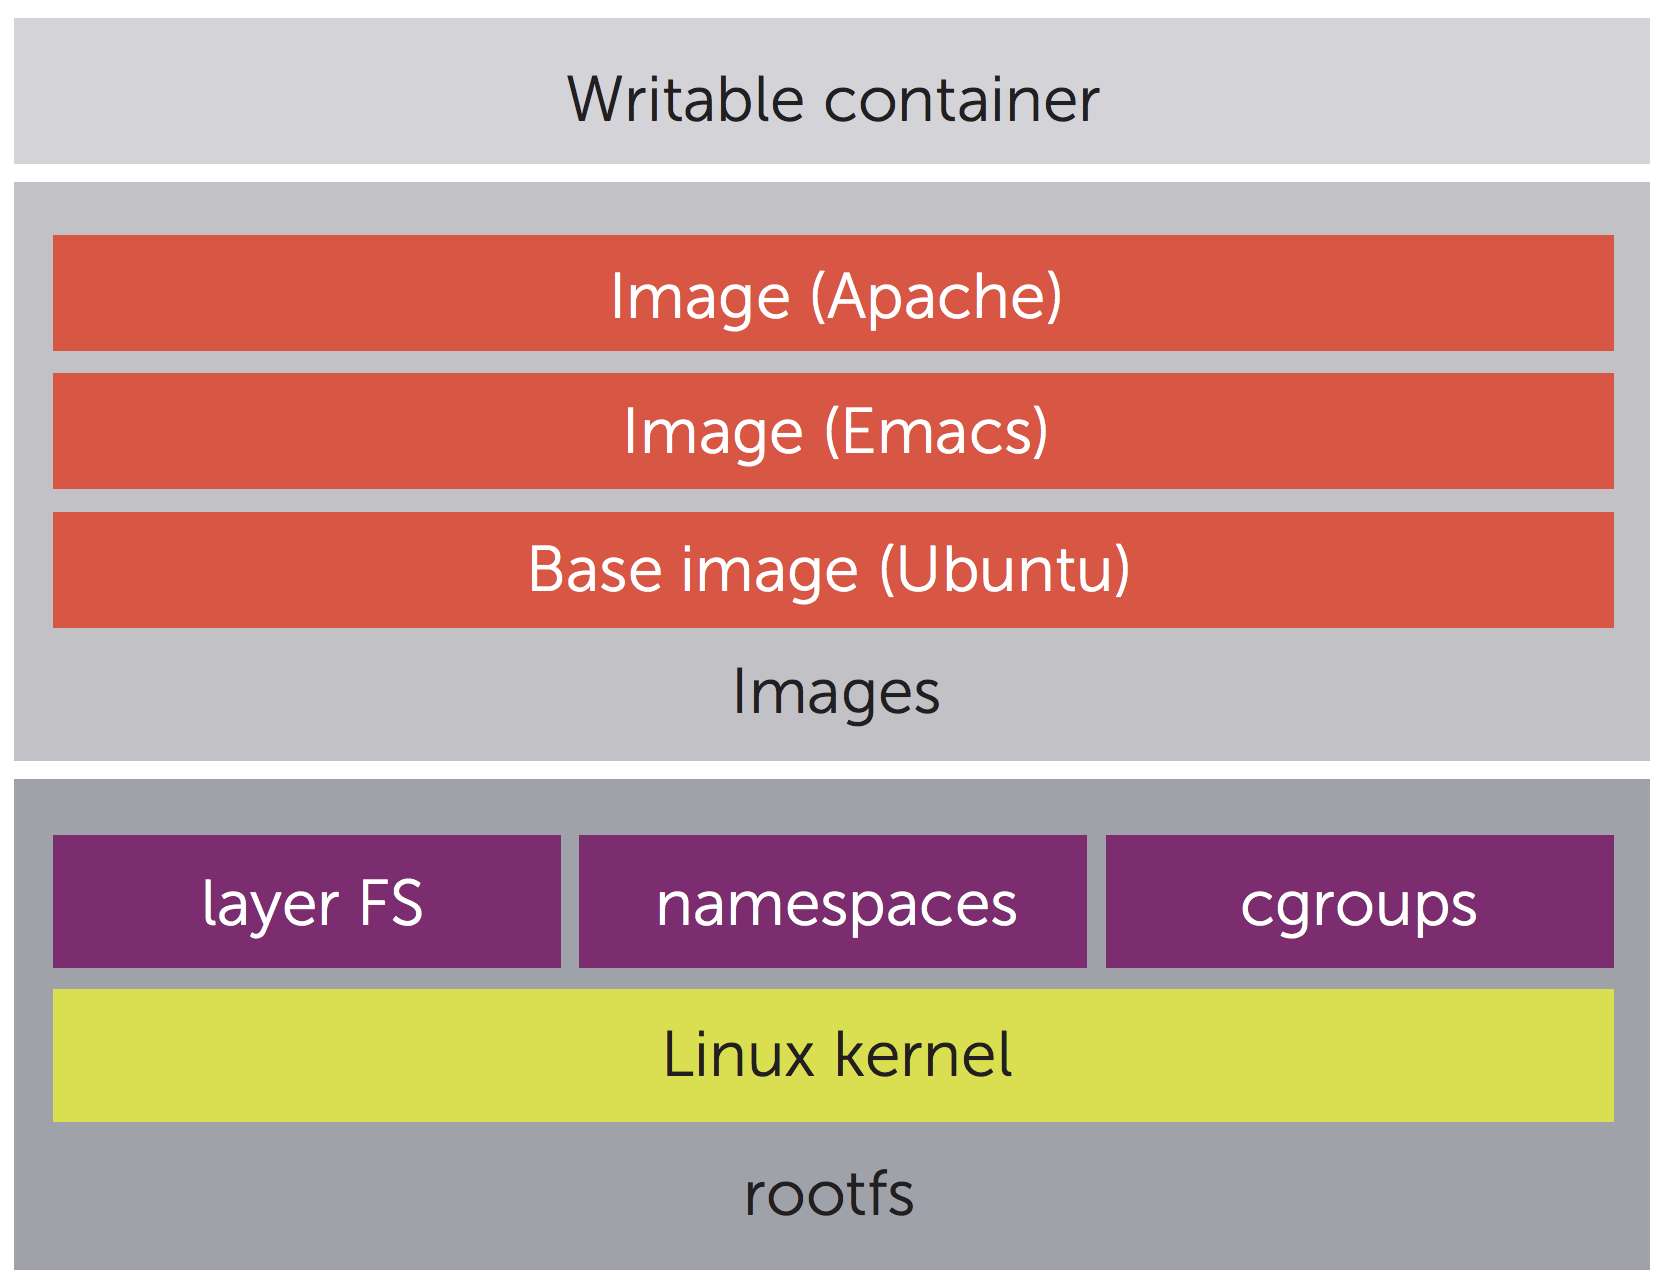
\includegraphics[width=0.5\textwidth]{chapter-background/docker-layers.png}
\end{figure}

\section{Container Orchestration}
Container technologies such as Docker offer advanced features to use containers in production. These solutions often offer deployment of applications limited to single machines. However, applications offered by  SaaS providers may include multiple different containers working together running on a cluster of nodes. Container orchestration (CO) systems allow deployment and management of containers at scale. Popular orchestration engines are Kubernetes, Docker Swarm and Mesos Marathon.
\subsection{Key capabilities of a container orchestration platform}
The task of a container orchestration (CO) platform is not limited to the initial deployment but the entire life-cycle of multiple containers. The goal of CO is to simplify cluster management while ensuring fault tolerance, availability, scalability and reliability. Allowing users to benefit from the complete potential of containers. In order to meet this goal, CO platform must at least offer the following key capabilities.~\cite{khan2017key}
\paragraph{Cluster state management and scheduling}
A cluster can be composed out of multiple virtualized or physical instances. Running containers on top of these instances and recover from failures requires a stable cluster. State management encapsulates various tasks such as flexible scheduling, re-partitioning of resources and data and propagating of dependent system changes.~\cite{khan2017key} 
\paragraph{High availability and fault tolerance}
A container orchestration platform must ensure high availability and fault tolerance in order to be useful for application developers. Most platforms therefor employ design principles of reliability engineering e.g., single point of failure elimination, failure detection or load balancing.~\cite{khan2017key}
\paragraph{Security}
Containers executing on top of the platform essentially form untrusted entities, with potentially malicious intentions, a high security standard is required. The standard should include: container images sanity check policies, access control for both containers and users, and techniques to minimize the container attack surface.~\cite{khan2017key}  
\paragraph{Simplified networking}
Containers must be able to communicate across nodes in  an efficient and secure manner. This requires the mapping of allocated host ports to containers. The overhead corresponding to this mapping intensifies at scale. The CO platform should thus provide a flexible, secure and scalable solution for networking.~\cite{khan2017key}
\paragraph{Service discovery}
The large number of services present in a cluster need to be able to communicate with each other. In traditional clusters services were handled as pets (i.e, having static names, IP addresses), however, in dynamic environments such as container orchestration platforms, they are regarded as cattle. The CO platform must provide mechanisms for addressing/labeling/grouping and service discovery.~\cite{khan2017key} 
\paragraph{Monitoring and governance}
The container orchestration platform needs to support traditional monitoring techniques such as logging, resource usage and network trace-routes. Monitoring must be possible at both the level of the underlying infrastructure and the containers themselves.~\cite{khan2017key}
\paragraph{Integrating for continuous integration and delivery}
Software development teams should be able to integrate the CO platform within their employed continuous integration and delivery (CI/CD) pipeline. The CO platform should contain mechanisms for rolling updates, rollbacks, etc.~\cite{khan2017key}


\subsection{Kubernetes}
Kubernetes~\cite{kubernetes}, commonly referred to as K8,  is one of the most popular and adopted orchestration systems. It is an open-source project led by Google. Kubernetes is Google's solution for the growing demand of container deployments by external developers in its public business cloud and is based upon its predecessors  Borg~\cite{verma2015large} and Omega~\cite{schwarzkopf2013omega} that have been used to schedule the internal Google workload. Its main design goal is formulated as:\textit{ "to make it easy to deploy and manage complex distributed systems, while still benefiting from the improved utilization that containers enable~\cite{Burns:2016:BOK:2930840.2890784}"}.  \\\\
\noindent To achieve the above stated goal Kubernetes introduces a number of concepts for both containers and cluster resources. It implements the infrastructure as code model  by provides an abstraction layer on top of the physical infrastructure~\cite{hermanns2015current}. It allows to setup and manage container infrastructure by the configuration of these introduced concepts via a REST API or declarative YAML configuration files. Below the most relevant concepts are introduced.
\subsubsection{Kubernetes concepts}
\textbf{Pods.}  A pod is the smallest unit of deployment within Kubernetes. It is a group of one or more containers that logically belong together.   A pod and thus its containers run on the same node. They share the same network, storage and context (Linux namespaces, cgroups). A pod gets assigned a unique IP address. Pods are not self-healing meaning when an error occurs within the pod or during scheduling. It will be deleted. Due to this short life cycle using a single pod resource and its assigned IP address for applications is impractical. Kubernetes handles this by employing controllers and services.~\cite{pods}\\\\
\textbf{Deployments.}  A Deployment controller manages a pod or a ReplicaSet of pods. A ReplicaSet allows pods to be replicated across multiple nodes. A Deployment object is used to specify the desired state of pods (e.g. number of replica's). A deployment, in addition, allows for declarative updates. These updates can be used to change the number of container replicas of a ReplicaSet or to update a specific container image within the pod.  The Deployment controller changes the actual state to the desired state described by the update.~\cite{deployments}
\\\\
\textbf{Services.}  Services offer a solution for the short life cycle of pods (and their IP addresses). Services within Kubernetes offer a manner to expose a ReplicaSet of Pods via a unique name, stable IP address, network policy and ports. To determine which set of pods is targeted by a service, Kubernetes employs a Label selector. Labels are the core grouping primitive of Kubernetes and unlike names and UIDs do not offer uniqueness.\\  A Service can be exposed outside the cluster by using an external load balancer or by specifying a NodePort. When using a Nodeport each node within the cluster will expose the port and forward request into the service.~\cite{services}
\\\\
\textbf{Namespaces.}  Namespaces allow to partition resources of a physical cluster among multiple user organizations. Each namespace gets a share of the resources of the cluster, via resource quotas. Resource quotas are supported for CPU, memory and persistent volumes.~\cite{namespaces-k8}
\\\\
\textbf{Resource limits.}  Kubernetes allows the allocation of compute resources of both containers and Namespaces by the means of resource limits. These limits can be soft (limit) and hard (request) limits. A Request specifies the quantity of resource that is guaranteed to the container. A limit specifies the maximum quantity allocated to the container. When the requested resource quantities of a container are less than its limit, the container may be allocated additional resources if there are unallocated resources available.  The current supported compute resources are CPU, memory and storage within the root partition of the local node. Within a Pod it is possible to specify both request and limit for each container. When request and limits are specified, the scheduler will use them for both scheduling and eviction (when node capacity is reached) decisions.~\cite{kubresources}
\subsubsection{Kubernetes architecture}
The basic architecture of Kubernetes is illustrated in Figure~\ref{fig:kubarch}. A client-server architecture is employed in which master and node setups are deployed on different machines. Below the different components that build up the architecture are briefly explained. 
\paragraph{API Server.} The API server is responsible for the configuration and validation of API objects (pods, deployments, services,...). It offers communication on cluster state via a REST interface for both components and administrators.~\cite{kubernetes-api-server}
\paragraph{Controller manager.} The controller manager is responsible for managing several core control loops part of Kubernetes. A control loop uses the API server to observe the shared state of the cluster and attempts to move to the desired state via configuration changes.~\cite{kubernetes-controller-manager}
\paragraph{Scheduler.} The task of assigning pods to nodes is the responsibility of the scheduler component.  The scheduler attempts to do a reasonable placement based on resource and quality of service requirements (e.g., not place a pod on a node with insufficient resources). It is  possible for users to control the placement of pods via NodeSelector tags or affinity and anti-affinity constraints in the configuration file.~\cite{kubernetes-pods-to-nodes,kubernetes-scheduler}
\\\\In addition it is possible to assign Quality of Service (QoS) classes to pods. These are used by Kubernetes in the decision process about scheduling and eviction of pods. Currently, Kubernetes supports three types of classes: guaranteed, burstable and best-effort. In decreasing order of priority (i.e., most likely to be killed in the case of resource shortages). The QoS classes are assigned to pods based on the presence of request and limit specifications of resources in their configuration files.~\cite{kubernetes-qos}


\paragraph{Kubelet.} The kubelet component is an agent running on each node. It is responsible for running and maintaining pods on its residing node. The set of maintained pods is described in the form of PodSpecs (mainly received via the API-server).~\cite{kubernetes-kubelet}
\paragraph{Kube-proxy.} The kube-proxy daemon provides a simple network proxy for the services on each node. It enables forwarding of requests to the correct containers and can provide primitive load balancing.~\cite{kubernetes-kubeproxy}
\begin{figure}[H]
\caption{Kubernetes architecture}
\centering
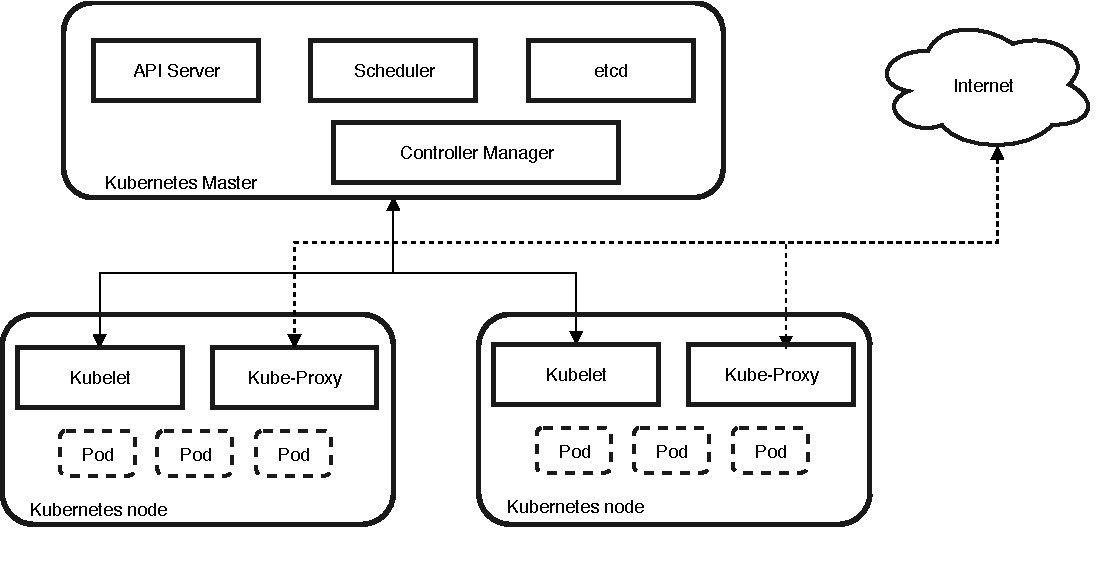
\includegraphics[width=0.8\textwidth]{chapter-background/kubernetes-architecture-diagram.pdf}
\label{fig:kubarch}
\end{figure}
 
 
 
 
 
 
 
 
 
 \section{Performance evaluation}
As discussed in previous sections, SaaS providers employ multi-tenancy to improve  cost efficiency and offer several performance guarantees to their customers in the form of SLOs. An unavoidable consequence of multi-tenancy is the need to support a growing number of users in a single system. Providers need to have a clear insight into the \textit{scalability} of their systems. However, scalability is a difficult thing to define, let alone quantify. Citing the words of  Dr. Neil J. Gunther:  \textit{"if you can't quantify it, you can't guarantee it"}.~\cite{perfdynamics}

\subsection{The Universal Scalability Law}
\label{section-USL}
Dr. Neil J. Gunther provides a formal definition of scalability: \textit{"scalability can be defined as a mathematical function, a relationship between independent and dependent variables (input and output)"~\cite{perfdynamics}}. The Universal Scalability Law (USL) by Dr. Neil J. Gunther is presented in Equation~\ref{USL}. It computes the relative capacity $C(N)$ at a load of $N$ users. Relative capacity is the normalized throughput.
\begin{equation}
\label{USL}
C(N) = \frac{\gamma~N}{1 + \alpha~(N-1) + \beta~N~(N-1)}
\end{equation}

The Universal Scalability Law incorporates factors that contribute to the sublinearly scalability of most systems. Namely, \textbf{concurrency} ($\gamma$), \textbf{contention} ($\alpha$) and \textbf{coherency} ($\beta$) as explained below. Their impact is visualized in Figure~\ref{fig:usl-impact}.

\begin{itemize}
    \item \textbf{Concurrency}($\gamma$): $\gamma$ defines the slope if the system was linearly scaling i.e., $C(N) = \gamma N$. It has been referred to as the \textit{coefficient of performance} by~\cite{schwarz2015practical}.
    \item \textbf{Contention} ($ \alpha $) : When scaling most systems parallelism while be limited at some point by contention (i.e., waiting or queuing for shared resources). The maximum speedup by parallelism is limited by the serialized portion ($\alpha$) of the work~\cite{schwarz2015practical}. 
    \item \textbf{Coherency} ($\beta$): created by crosstalk between components. Because crosstalk is possible between each pair of components in the system, the penalty grows quadratic $N(N-1)$.~\cite{schwarz2015practical}
    
\end{itemize}

\begin{figure}
    \centering
    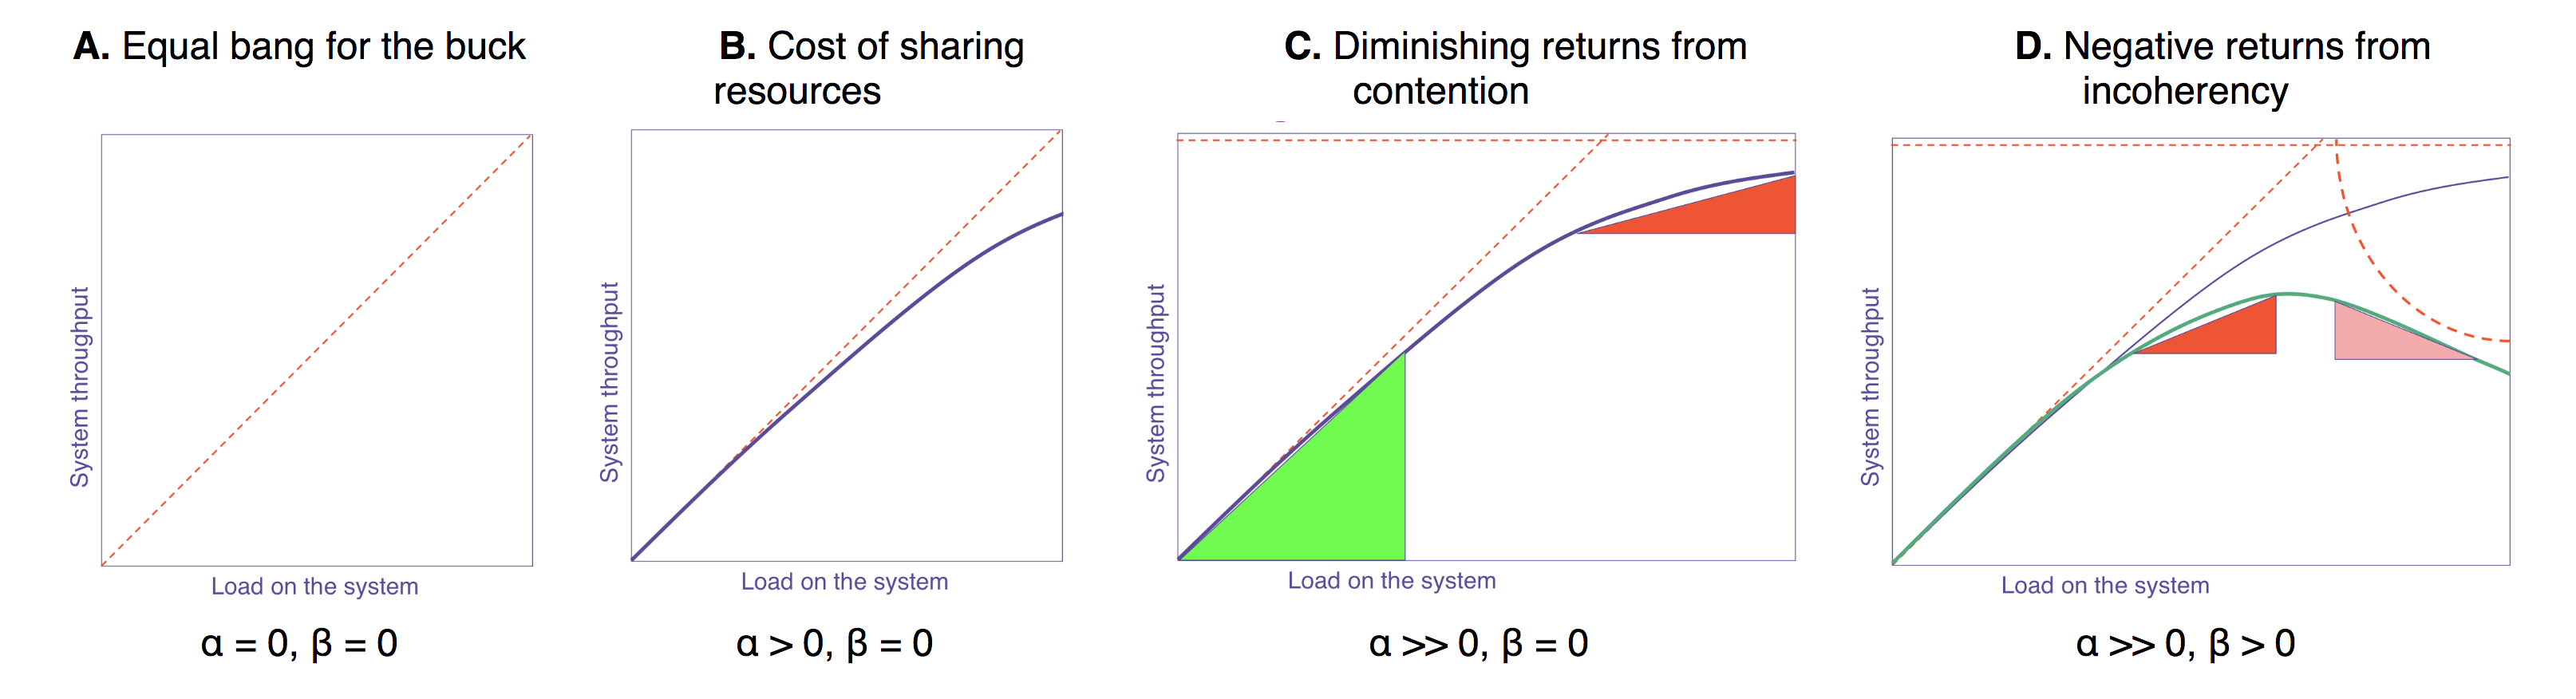
\includegraphics[width=1.1\textwidth]{chapter-evaluation/usl-impact}
    \caption{The impact of different USL coefficients on scalability.~\cite{perfdynamics}}
    \label{fig:usl-impact}
\end{figure}

\subsubsection{USL in practice}
USL can provide insights into a system's scalability pains via  values of the concurrency, contention and coherency coefficients. These can be obtained by collecting a dataset of measurements of the system, system load $N$ and corresponding throughput, and using a statistical technique such as nonlinear least square regression which fits the USL to the dataset.~\cite{schwarz2015practical,heyman2014scalability}

\subsection{Little's law}
\label{sec:little}
The Universal Law of Scalability serves as an alternative for the often less intuitive queuing models frequently used for modeling scalability. It omits the need to know the service time for every queue in the performance model in order to predict the response time or latency~\cite{perfdynamics}. Nevertheless, queuing theorem and its lemmas such as Little's Law can provide useful insights into performance modeling.\\\\
John D.C Little's Law~\cite{little2008little} states the following for stable systems: 
\begin{displayquote}
\textit{"The average number of items in a queuing system equals the average rate at which items arrive multiplied by the average time that an item spends in the system.\cite{little2008little}"}
\end{displayquote}
\begin{equation}
\label{littleslaw}
L = \lambda~W
\end{equation}
\begin{equation}
\label{llsys}
N = X~Rt
\end{equation}
Equation~\ref{littleslaw} shows Little's law, below its terms and its applicability to web services (Equation~\ref{llsys}) are explained:
\begin{itemize}
    \item \textbf{$L$}:  Average number of items in the system. For a web service this is represented by the average number of concurrent users in the system $N$.
    \item \textbf{$\lambda$}: Long-term average arrival rate of items in the system per time unit. Little's law assumes a stable system for which the arrival rate and exit rate are identical. In a web service this is represented by the throughput $X$.
    \item \textbf{$W$}: Average waiting time of an item in the system, queuing time and service time combined. This is represented by the response time $Rt$ or latency of a request in a web service. When dealing with a system involving think time (e.g., after the response from a web service, a user needs time to think about his/her next request), $(Rt + Zt)$ is used. 
\end{itemize}

\subsubsection{Workload generator validation}
Developers employ software tools (JMeter~\cite{jmeter}, Locust~\cite{locust}, etc.)  to simulate a workload and test the performance of a system. A workload is a set of actions that represent the behavior of a client in the system. It is part of the test plan stating the number of concurrent users $N$ executing the workload for a specified period of time.\\\\
The results of a performance test are typically expressed in throughput $X$ and response time $Rt$. Using Little's law it is possible to validate these results. For example, a test plan of 1000 concurrent users $N$ results in a throughput of 50 requests per second and an average response time of 15 seconds. Following Little's law, a concurrence of only 750 users was reached, instead of the specified 1000. Little's law can thus be used to check if a workload generator works as specified.\\\\
Alternatively, if the average throughput and response time for a production system are known, Little's law can be used to correctly draw up a test plan.

\subsubsection{Response time or latency?}
Performance can either be measured in throughput or latency, both are correct but offer a different point of view. System performance is typically expressed in throughput: "The system can handle a million operations per second". However, users care more about their personal experience with a system which is influenced by the average latency of their request.~\cite{schwarz2015practical} \\\\
Figure~\ref{fig:ls_vs_tp} shows the relation between the average latency and throughput of a database under increasing load $N$. In this case, latency is kept stable by increasing the throughput with the increasing load up to a certain point.  A bottleneck caps the throughput of the systems and by Little's law for an increasing load and constant throughput, the latency must increase.~\cite{latvsthrough} \\\\
However in other systems, as discussed in Section~\ref{section-USL}, an increasing load might induce a diminishing result on the system's throughput. Following Little's law a decreasing throughput results in a higher latency under the same load. \\\\
Thus, for stable systems by Little's law,  the USL can be reformulated in terms of latency instead of throughput. Equation~\ref{USL-2} shows this reformulation.~\cite{schwarz2015practical}
\begin{equation}
\label{USL-2}
Latency(N) = \frac{1 + \alpha~(N-1) + \beta~N~(N-1)}{\gamma}
\end{equation}


\begin{figure}[H]
    \centering
    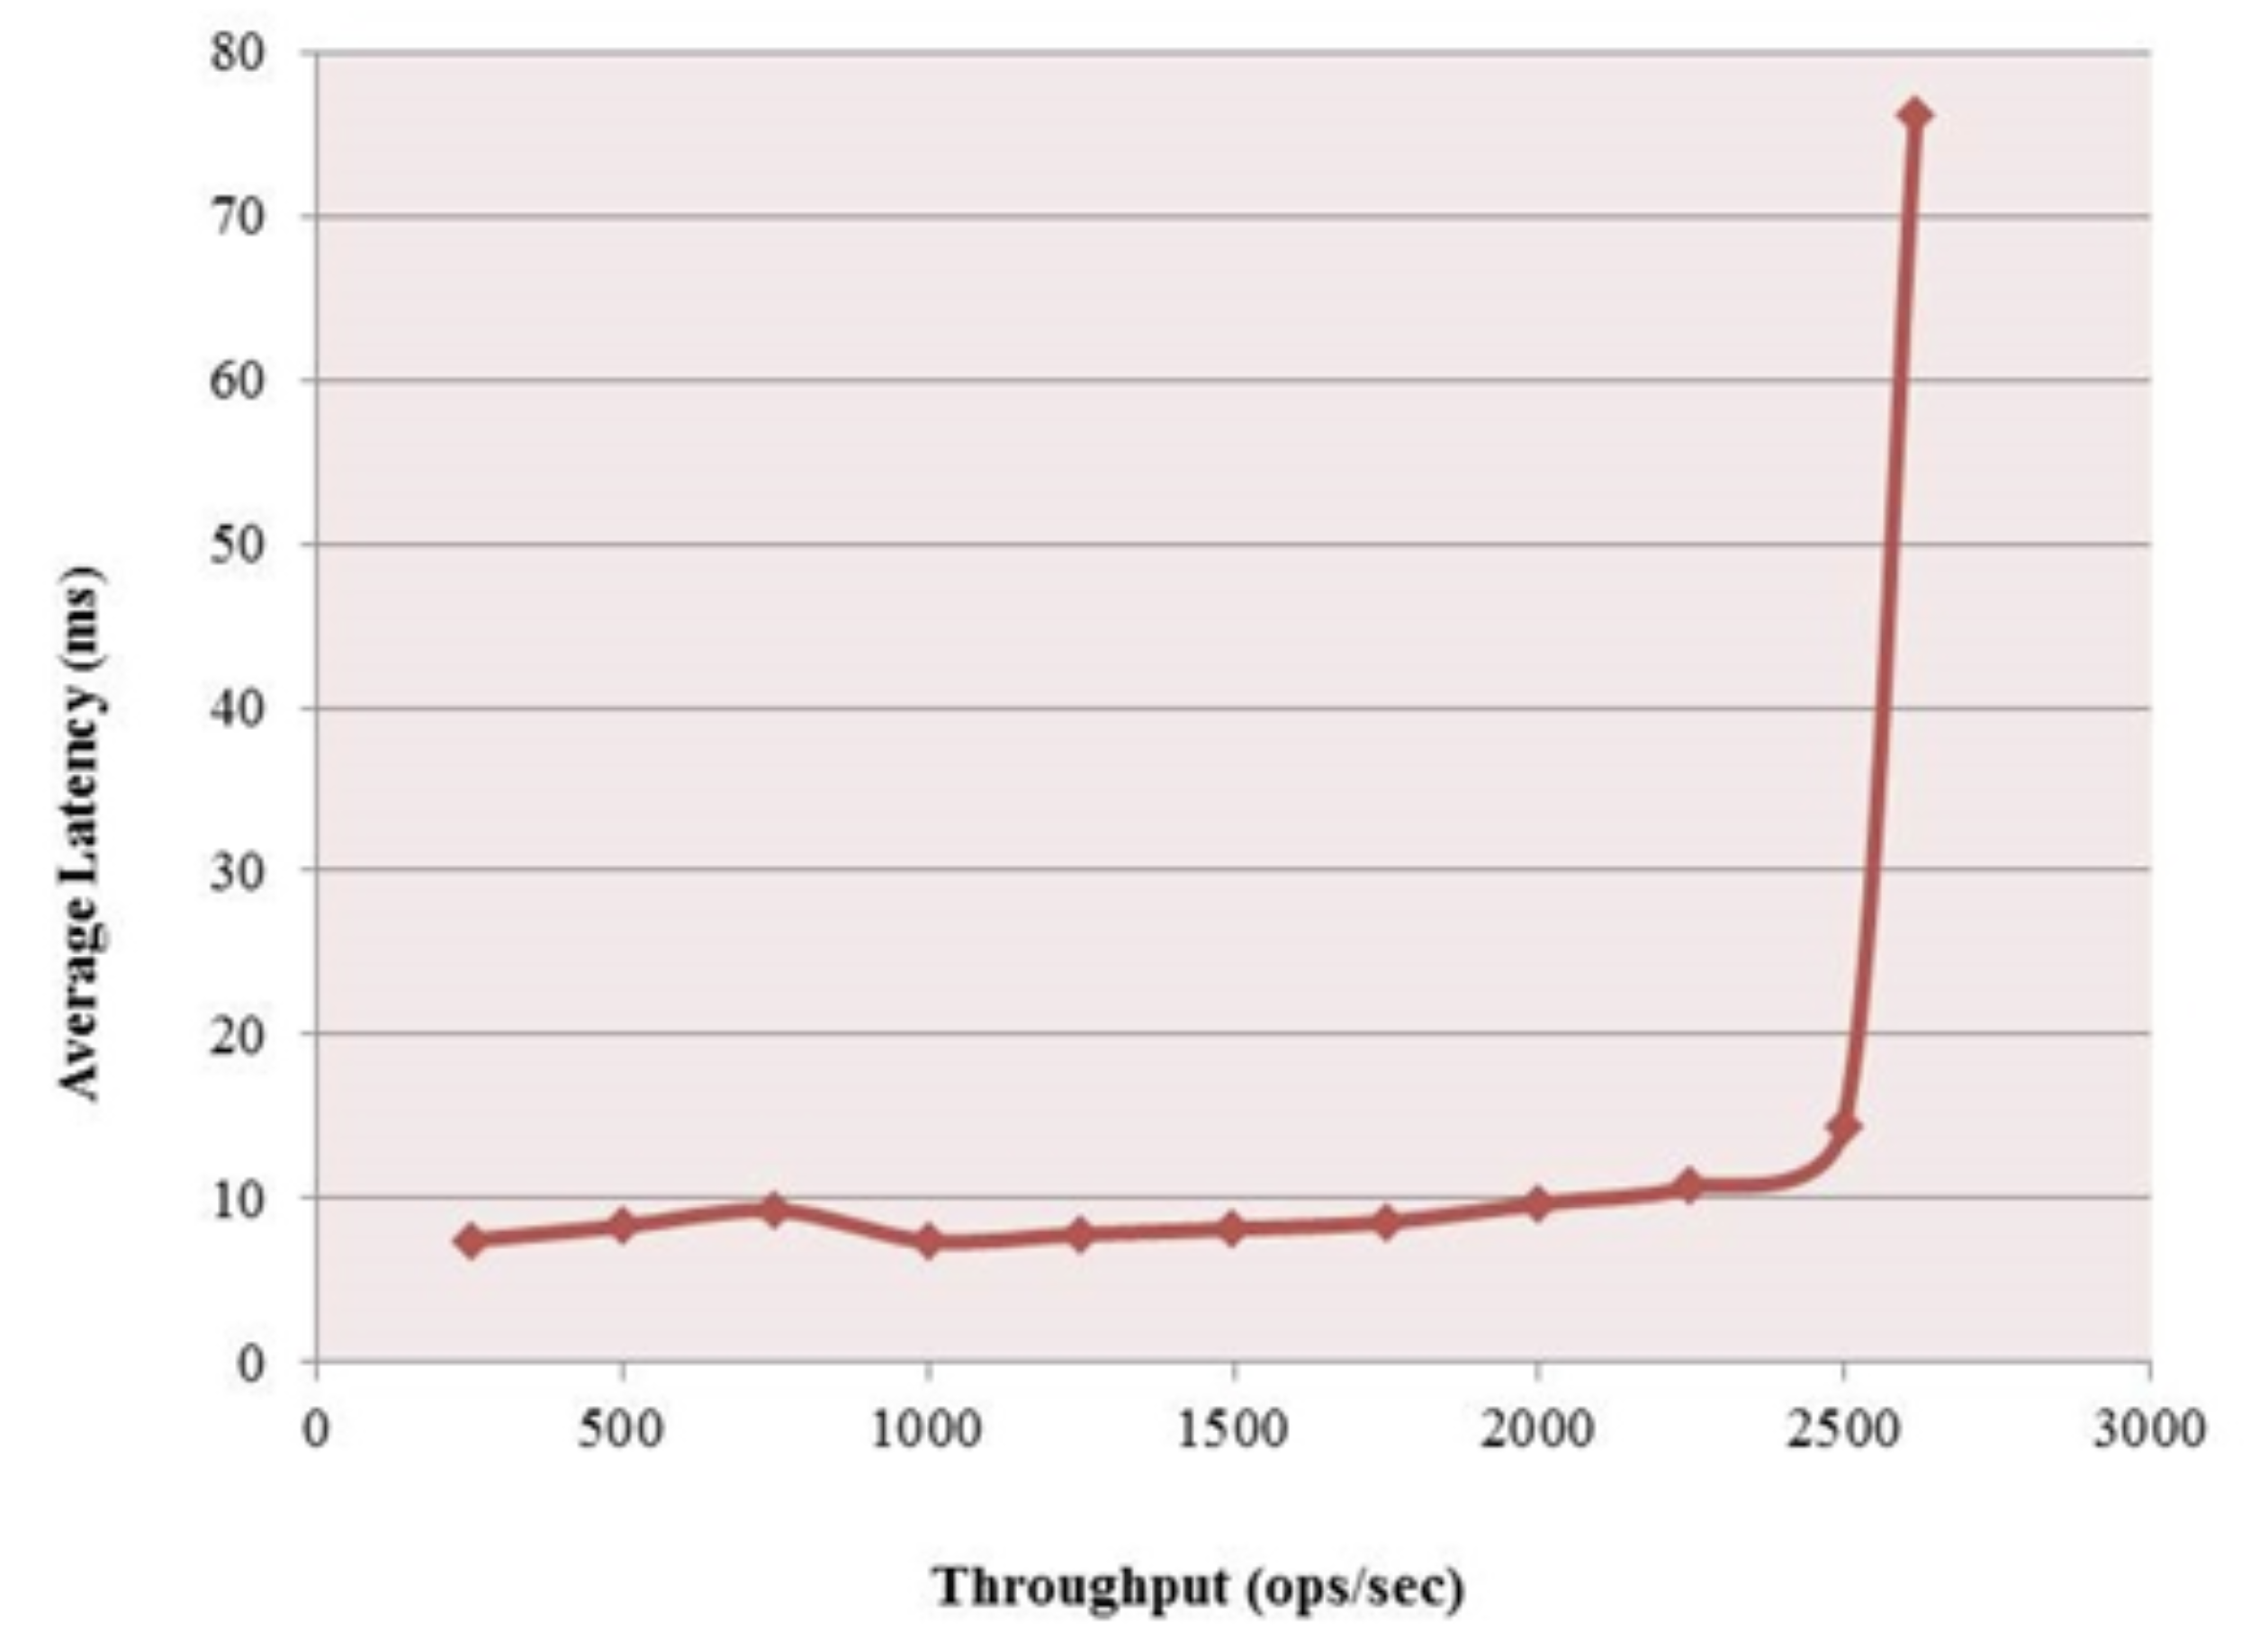
\includegraphics[width=0.8\textwidth]{chapter-evaluation/ls_vs_th}
    \caption{Relation average latency vs. throughput for database benchmark with increasing load.~\cite{latvsthrough}}
    \label{fig:ls_vs_tp}
\end{figure}
% \chapter{The First Chapter}
\label{cha:1}
A chapter is a logical unit. It normally starts with an introduction, which
you are reading now. The last topic of the chapter holds the conclusion.

\section{The First Topic of the Chapter}
First comes the introduction to this topic.

\lipsum[55]

\subsection{An item}
Please don't abuse enumerations: short enumerations shouldn't use
``\verb|itemize|'' or ``\texttt{enumerate}'' environments.
So \emph{never write}: 
\begin{quote}
  The Eiffel tower has three floors:
  \begin{itemize}
  \item the first one;
  \item the second one;
  \item the third one.
  \end{itemize}
\end{quote}
But write:
\begin{quote}
  The Eiffel tower has three floors: the first one, the second one, and the
  third one.
\end{quote}

\section{A Second Topic}
\lipsum[64]

\subsection{Another item}
\lipsum[56-57]

\section{Conclusion}
The final section of the chapter gives an overview of the important results
of this chapter. This implies that the introductory chapter and the
concluding chapter don't need a conclusion.

\lipsum[66]

%%% Local Variables: 
%%% mode: latex
%%% TeX-master: "thesis"
%%% End: 

% \chapter{The Next Chapter}
\label{cha:2}
\lipsum[77]

\section{The First Topic of this Chapter}
\lipsum[78]

\subsection{An item}
A master's thesis is never an isolated work. This means that your text must
contain references. On-line documents\cite{wiki} as well as
books\cite{pratchett06:_good_omens} can be referenced.

\section{Figures}
Figures are used to add illustrations to the text. The \fref{fig:logo} shows
the KU~Leuven logo as an illustration.
\begin{figure}
  \centering
  
\includegraphics{config/logokul}
  \caption{The KU~Leuven logo.}
  \label{fig:logo}
\end{figure}

\section{Tables}
Tables are used to present data neatly arranged. A table is normally
not a spreadsheet! Compare \tref{tab:wrong} en \tref{tab:ok}: which table do
you prefer?

\begin{table}
  \centering
  \begin{tabular}{||l|lr||} \hline
    gnats     & gram      & \$13.65 \\ \cline{2-3}
              & each      & .01 \\ \hline
    gnu       & stuffed   & 92.50 \\ \cline{1-1} \cline{3-3}
    emu       &           & 33.33 \\ \hline
    armadillo & frozen    & 8.99 \\ \hline
  \end{tabular}
  \caption{A table with the wrong layout.}
  \label{tab:wrong}
\end{table}

\begin{table}
  \centering
  \begin{tabular}{@{}llr@{}} \toprule
    \multicolumn{2}{c}{Item} \\ \cmidrule(r){1-2}
    Animal    & Description & Price (\$)\\ \midrule
    Gnat      & per gram    & 13.65 \\
              & each        & 0.01 \\
    Gnu       & stuffed     & 92.50 \\
    Emu       & stuffed     & 33.33 \\
    Armadillo & frozen      & 8.99 \\ \bottomrule
  \end{tabular}
  \caption{A table with the correct layout.}
  \label{tab:ok}
\end{table}

\section{Lorem Ipsum}
This section is added to check headers and footers. So this chapter must at
least contain three pages. To make sure that we get the required amount,
the \textsf{lipsum} package isn't used but the text is put directly in the
text.

\subsection{Lorem ipsum dolor sit amet, consectetur adipiscing elit}
Sed nec tortor id felis tristique sodales. Nulla nec massa eu dui fermentum
tincidunt. Integer ullamcorper ante eget eros posuere faucibus. Nam id
ligula ut augue pulvinar vulputate id at purus. Aenean condimentum tortor
eu mi placerat eget eleifend massa mollis. Nam est mi, sagittis quis
euismod eget, sagittis in nibh. Proin elit turpis, aliquam et imperdiet
sed, volutpat eu turpis.

Pellentesque vel enim tellus, vitae egestas turpis. Praesent malesuada elit
non nisi sollicitudin non blandit lacus tincidunt. Morbi blandit urna at
lectus ornare laoreet. Suspendisse turpis diam, lobortis dictum luctus
quis, commodo at lorem. Integer lacinia convallis ultricies. Sed quis augue
neque, eu malesuada arcu. Nullam vehicula, purus vitae sagittis pulvinar,
erat eros semper massa, eu egestas nibh erat quis magna. Cras pellentesque,
nisl eu dapibus volutpat, urna augue ornare quam, quis egestas lectus nulla
a lectus.

Vivamus dictum libero in massa cursus sed vulputate eros imperdiet. Donec
lacinia, libero ac lobortis egestas, nibh dui ornare arcu, luctus porttitor
velit massa sit amet quam. Maecenas scelerisque laoreet diam, vitae congue
quam adipiscing vitae. Aliquam cursus nisl a leo convallis eleifend
fermentum massa porta. Nunc libero quam, dapibus dapibus molestie sit amet,
faucibus vel nunc.

\subsection{Praesent auctor venenatis posuere}
Sed tellus augue, molestie in pulvinar lacinia, dapibus non ipsum. Fusce
vitae mi vitae enim ullamcorper hendrerit eu malesuada est. Proin iaculis
ante sed nibh tincidunt vel interdum libero posuere. Vivamus accumsan metus
quis felis congue suscipit dapibus enim mattis. Fusce mattis tortor eget
ipsum interdum sagittis auctor id metus.

Integer diam lacus, pharetra sit amet tempor et, tristique non lorem.
Aenean auctor, nisi eu interdum fermentum, lectus massa adipiscing elit,
sed facilisis orci odio a lectus. Proin mi nibh, tempus quis porta a,
viverra quis enim. In sollicitudin egestas libero, quis viverra velit
molestie eget. Nulla rhoncus, dolor a mollis vestibulum, lacus elit semper
nisi, nec sollicitudin sem urna eu magna. Nunc sed est urna, euismod congue
mi.

\subsection{Cras vulputate ultricies venenatis}
Vivamus eros urna, sodales accumsan semper vel, lobortis sit amet mauris.
Etiam condimentum eleifend lorem, ullamcorper ornare lectus aliquet vitae.
Praesent massa enim, interdum sit amet semper et, venenatis ut elit.
Quisque faucibus, quam ac lacinia imperdiet, nulla neque elementum purus,
tempus rutrum justo massa porta sapien. Vestibulum ante ipsum primis in
faucibus orci luctus et ultrices posuere cubilia Curae; Sed ultrices
interdum mi, et rhoncus sapien rutrum sed.

Duis elit orci, molestie quis sollicitudin sed, convallis non ante.
Maecenas tincidunt condimentum justo, et ultricies leo tristique vitae.
Vestibulum quis quam non lectus dapibus eleifend a vitae nibh. Nam nibh
justo, pharetra quis iaculis consequat, elementum quis justo. Etiam mollis
lacinia lacus, nec sollicitudin urna lobortis ac. Nulla facilisi.

Proin placerat risus eleifend erat ultricies placerat. Etiam rutrum magna
nec turpis euismod consectetur. Phasellus tortor odio, lacinia imperdiet
condimentum sed, faucibus commodo erat. Phasellus sed felis id ante
placerat ultrices. Aenean tempor justo in tortor volutpat eu auctor dolor
mollis. Aenean sit amet risus urna. Morbi viverra vehicula cursus.

\subsection{Donec nibh ante, consectetur et posuere id, tempus nec arcu}
Curabitur a tellus aliquet ipsum pellentesque scelerisque. Etiam congue,
risus et volutpat rutrum, est purus dapibus leo, non cursus metus felis
eget ligula. Vivamus facilisis tristique turpis, ut pretium lectus luctus
eleifend. Fusce magna sapien, ullamcorper vitae fringilla id, euismod quis
ante.

Phasellus volutpat, nunc et pharetra semper, sem justo adipiscing mauris,
id blandit magna quam et orci. Vestibulum a erat purus, ut molestie ante.
Vestibulum ante ipsum primis in faucibus orci luctus et ultrices posuere
cubilia Curae; Proin turpis diam, consequat ut ullamcorper ut, consequat eu
orci. Sed metus risus, fringilla nec interdum vel, interdum eu nunc.
Suspendisse vel sapien orci.

\subsection{Morbi et mauris tempus purus ornare vehicula}
Mauris sit amet diam quam, eget luctus purus. Sed faucibus, risus semper
eleifend iaculis, mi turpis bibendum nisl, quis cursus nibh nisl sit amet
ipsum. Vestibulum tempor urna vitae mi auctor malesuada eget non ligula.
Nullam convallis, diam vel ultrices auctor, eros eros egestas elit, sed
accumsan arcu tortor eget leo. Vestibulum orci purus, porttitor in pharetra
eget, tincidunt eget nisl. Nullam sit amet nulla dui, facilisis vestibulum
dui.

Donec faucibus facilisis mauris ac cursus. Duis rhoncus quam sed nisi
laoreet eu scelerisque massa tincidunt. Vivamus sit amet libero nec arcu
imperdiet tempor quis non libero. Sed consequat dignissim justo. Phasellus
ullamcorper, velit quis posuere vulputate, felis erat tincidunt mauris, at
vestibulum justo lectus et turpis. Maecenas lacinia convallis euismod.
Quisque egestas fermentum sapien eu dictum. Sed nec lacus in purus dictum
consequat quis vel nisl. Fusce non urna sem. Curabitur eu diam vitae elit
accumsan blandit. Nullam fermentum nunc et leo dictum laoreet. Donec semper
varius velit vel fringilla. Vivamus eu orci nunc.

\section{Conclusion}
The final section of the chapter gives an overview of the important results
of this chapter. This implies that the introductory chapter and the
concluding chapter don't need a conclusion.

\lipsum[66]

%%% Local Variables: 
%%% mode: latex
%%% TeX-master: "thesis"
%%% End: 

% % ... and so on until
% \chapter{The Final Chapter}
\label{cha:n}
\lipsum[79]

\section{The First Topic of this Chapter}
\subsection{Item 1}
\subsubsection{Sub-item 1}
\lipsum[80]

\subsubsection{Sub-item 2}
\lipsum[81]

\subsection{Item 2}
\lipsum[82]

\section{The Second Topic}
\lipsum[83-85]

\section{Conclusion}
\lipsum[86-88]

%%% Local Variables: 
%%% mode: latex
%%% TeX-master: "thesis"
%%% End: 

%\chapter{Conclusion}
\label{cha:conclusion}
The final chapter contains the overall conclusion. It also contains
suggestions for future work and industrial applications.

\lipsum[1-7]

%%% Local Variables: 
%%% mode: latex
%%% TeX-master: "thesis"
%%% End: 


% If you have appendices:
\appendixpage*          % if wanted
\appendix
\chapter{Background}
\label{ch:background}
This chapter discusses relevant background material for the thesis. The concepts, explored in this chapter, further clarify the relevance of the thesis and serve as building blocks for the remaining chapters. Starting from the adoption of the cloud computing paradigm, the chapter elaborates on how concepts such as multi-tenancy and virtualization via containerization push the limits of efficient resource utilization. Next, an in-depth overview of the open-source container orchestration platform Kubernetes is provided. Lastly, insights are provided into the universal scalability law and the applicability of Little's law for performance testing.
\section{Cloud computing}
Companies try to minimize the total cost of ownership by moving to cloud computing or utility computing. The cloud computing paradigm enables on-demand access to a shared pool of configurable compute resources (software applications, system software and hardware infrastructure)~\cite{WalravenStefan2015PPmf}. A service provider can provision the required resources from the cloud with minimal effort.  Within this paradigm, services are offered in real time over the internet in three different models~\cite{MellPeter2010TNDo,rimal2009taxonomy}. 
\begin{itemize}
\item \textit{Infrastructure as a Service (IaaS)} in which access is offered to virtual machines, network, data storage and other fundamental computing resources. The customer is able to deploy arbitrary software using these resources.\\\\
Examples: Digital Ocean, Microsoft Azure and Amazon Elastic Compute Cloud (EC2).
\item \textit{Platform as a service (PaaS)} offers customers a platform enabling easy and efficient deployment of applications (at scale) while abstracting the complexity of managing the underlying infrastructure. PaaS allows customers to solely focus on the development of their application.\\\\
Examples: Google app engine, Microsoft Azure and Heroku.
\item \textit{Software as a service (SaaS) } allows customers to make use of a specific application developed by a SaaS provider. Compared to the traditional use of software, the management and deployment is the task of the SaaS provider. In this strategy, common resources and a single instance of both the application and underlying database are used to support multiple customers simultaneously. \\\\
Examples: Google apps and Salesforce.
\end{itemize}

\section{Multi-tenancy}
\label{multi-tenancy}
The software as a service (SaaS) model offers applications to customers as an on-demand service. Providers of these applications try to leverage economies of scale by employing a multi-tenancy architectural design principle. The goal of multi-tenancy is to minimize the total cost of ownership for the provider by maximizing the sharing of resources among multiple customers organizations, referred to as tenants.~\cite{Walraven2015b} 
\subsection{Service Level Agreements}
By moving their core business functions to an entrusted cloud provider, cloud customers give up control of the underlying compute resources. It is vital for these tenants to obtain certain guarantees on the service delivered by the provider. 
A Service Level Agreement (SLA) is a formal contract between the SaaS provider and the tenant specifying both properties of the provided service and the expected behavior of the tenant. An SLA typically also contains a set of Service Level Objectives (SLOs). An SLO is a measurable characteristic of the service. An SLO is typically related to performance constraints (latency, throughput and deadlines) or availability (uptime percentage) of the service. Within the specification of an SLA a trade-off must often be made between expressiveness and usability. The SLA must cover all the expectations of a customer while remaining simple to weight, verify, evaluated and enforce~\cite{dillon2010cloud}.  Some typical examples of SLOs are shown below: 
\begin{itemize}
\item The application has a monthly uptime percentage of 99.95\%.
\item If the arrival rate of the tenant workload < X requests/s then a throughput T is guaranteed.
\end{itemize}
\subsection{Challenges}
While the goal of multi-tenancy is promising, sharing a cluster of dynamically provisioned nodes between multiple tenants imposes a number of challenges and requirements~\cite{TruyenEddy2016Taca}. 
\begin{itemize}
\item Performance isolation: the activities of one tenant should not be able to influence the service level delivered to other tenants. This requirement should be achieved during normal system load and when an aggressive tenant violates the terms of the SLA. 
\item QoS differentiation: the performance guarantees specified by an SLA can be individually customized for each tenant. A SaaS provider should be able to offer different subscriptions.
\item Flexible resource allocation for improved server consolidation: a SaaS provider employs a multi-tenant architecture to achieve a lower operational cost. This is partially achieved by planning the required node capacity based on the actual resource usage of tenants instead of the theoretical required capacity.  This can be further aided by the use of request schedulers allowing to distinguish between normal, passive and aggressive tenants. 
\end{itemize}
\subsection{Strategies}
To achieve multi-tenancy different strategies, each offering different trade-offs concerning operational costs and upfront application engineering costs, can be employed by the SaaS-provider~\cite{WalravenS.2011Amlf}. The strategies are illustrated in Figure~\ref{muti-tenant-strategies}.
\begin{itemize}
\item Multi-tenancy can be achieved at the level of the \textit{operating system}. In this strategy, a virtualization technology can be used to partition compute resources among multiple virtual machines. Each tenant is assigned an application instance running on a dedicated virtual machine. This approach offers both a higher level of performance isolation and lower upfront engineering costs but suffers from an inefficient utilization of resources.
\item In \textit{middleware-level multi-tenancy} a middleware platform is used to enable sharing compute resources between multiple tenants at the level of the operating system. An application instance is deployed on top of the middleware platform for each tenant. By not replicating the operating system for each tenant a higher level of cost efficiency can be achieved but an increased complexity in managing resources and  performance isolation is introduced. By tackling these problems at the level of the middleware a part of the engineering complexity is shifted to this level.
\item The most efficient resource utilization can be achieved by sharing application instances between multiple tenants. In \textit{Application-level} multi-tenancy achieving performance isolation is done by the application itself thereby increasing the engineering complexity and costs.
\end{itemize}


\begin{figure}[H]

\caption{Different strategies to achieve multi-tenancy~\cite{WalravenS.2011Amlf}.\label{muti-tenant-strategies} }
\centering
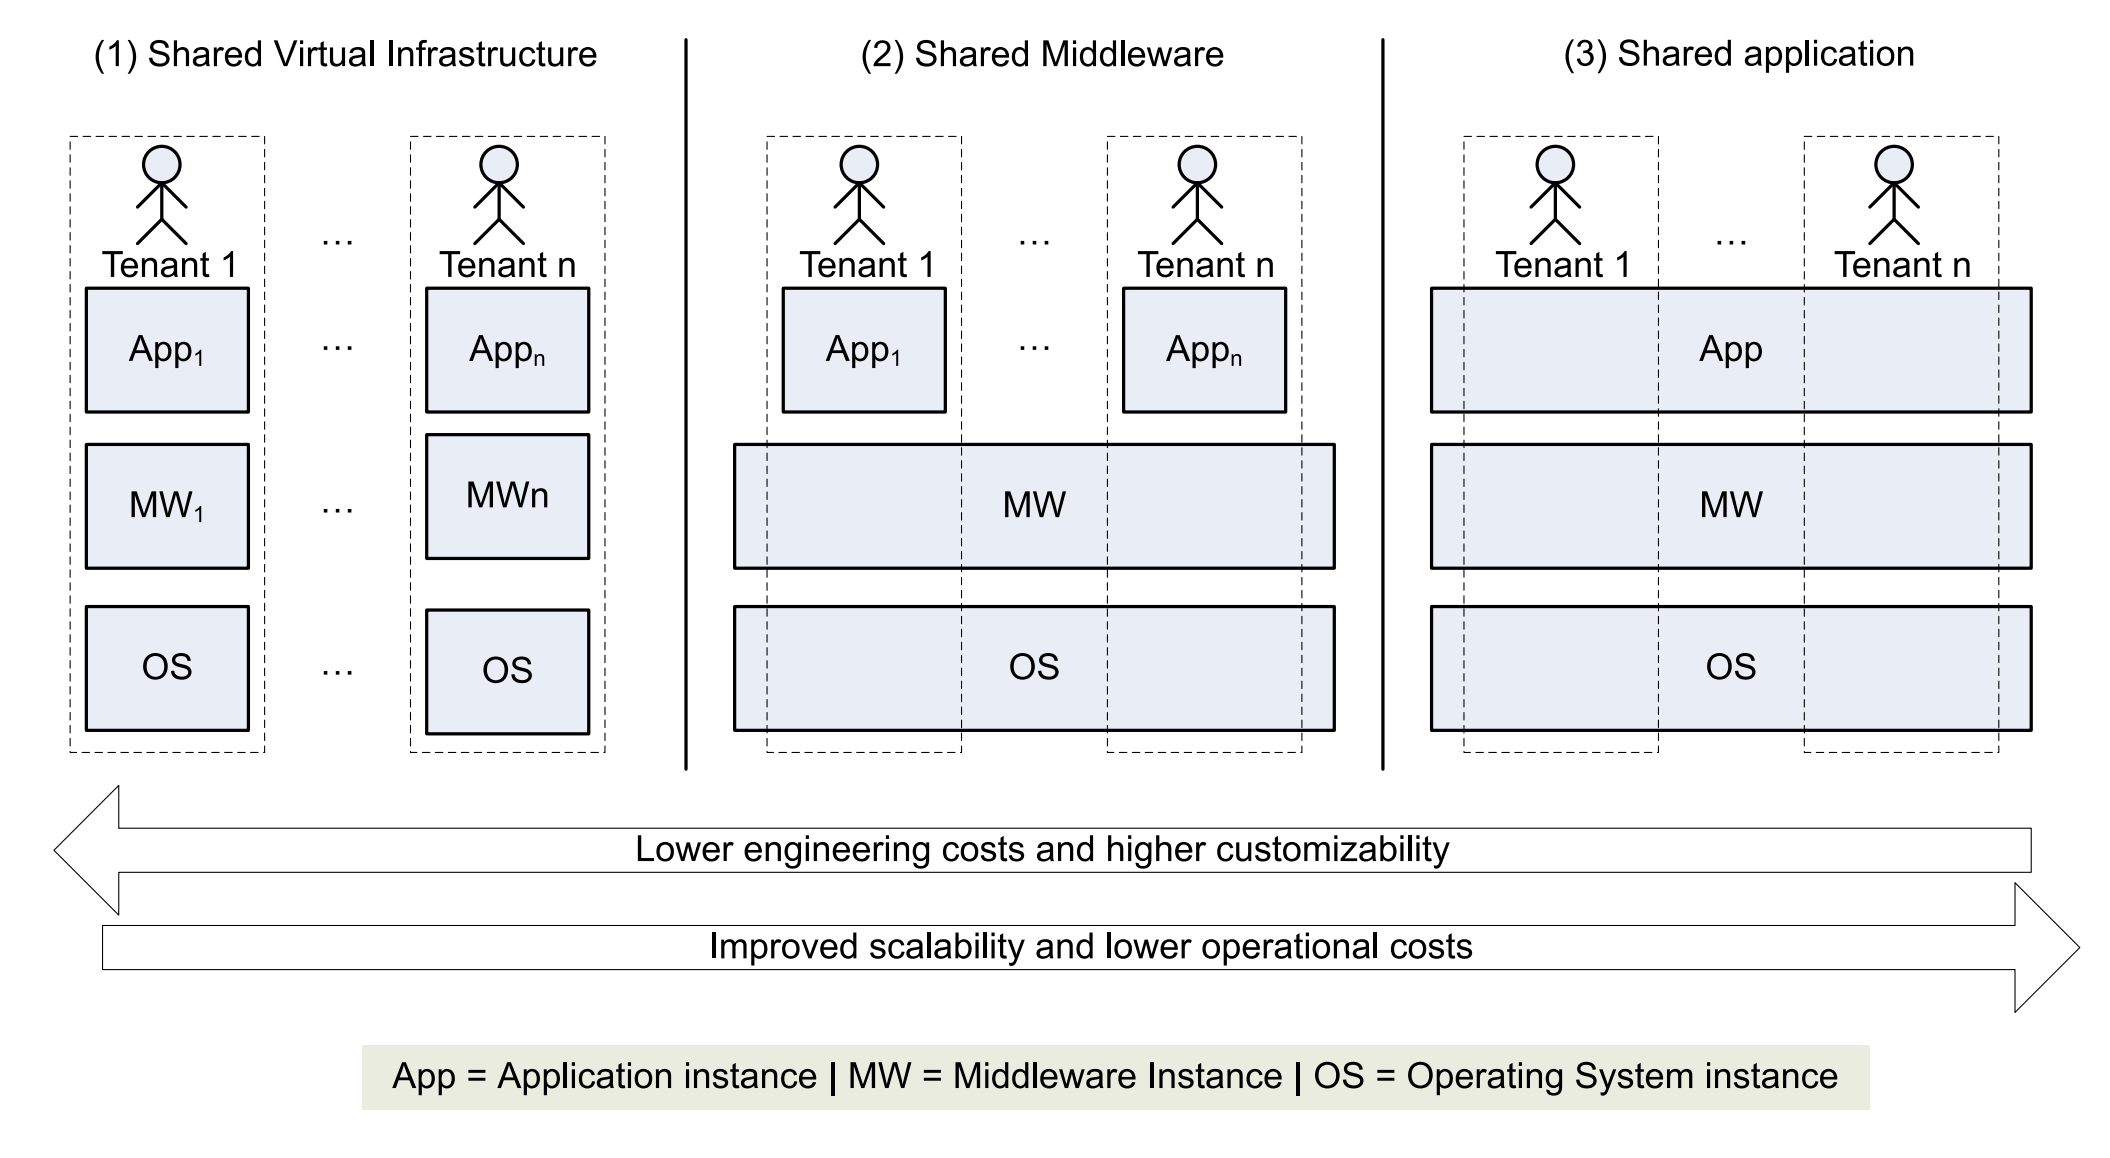
\includegraphics[width=0.65\textwidth]{chapter-background/muti-tenant-strategies.png}
\end{figure}


\section{Containerization}
Cloud providers rely on virtualization technology for the achievement of large-scale resource scaling. For more than a decade, virtual machines (VMs) have been the backbone of a provider's infrastructure offering hardware independence, availability, isolation and security~\cite{xavier2013performance}. More recently, containers a more lightweight virtualization technology have made advances in their multi-tenant capabilities and have seen an increase in adoption by providers~\cite{pahl2015containerization}. Both are discussed in this section.
\subsection{Virtualization technology}
In cloud environments, virtualization technology is used for flexible and dynamic allocation of physical resources to virtualized applications and to achieve multi-tenancy by sharing a physical server among multiple applications. In data centers virtualization is commonly used at the \textit{hardware level} and \textit{operating system level} to deploy and manage virtual machines and applications at scale~\cite{SharmaPrateek2016CaVM}. \\\\
Hardware level virtualization uses a hypervisor on a server to create virtual machines. Each virtual machine provides an abstraction of a physical machine and runs an independent operating system with applications. The hypervisor is responsible for resource allocation and performance isolation.\\\\
Operating system level virtualization allows resources to be shared at the level of the OS. Virtual machines running at the OS level are referred to as containers. Isolation, abstraction and resource allocation of containers is performed by the OS kernel of the host OS. By sharing the OS kernel among multiple containers, containers are regarded as a more lightweight virtualization technology. Containers only contain the application and its dependencies.\\\\
Linux containers (LXC)~\cite{lxc} employ different mechanisms of the Linux kernel to achieve resource isolation, namely control groups and namespaces.
\begin{itemize}
    \item \textbf{Cgroups}~\cite{cgroups} allow for fine-grained control of the allocation of system resources (CPU time, system memory, network bandwidth) among processes and process groups. For example, it is possible to limit or prioritize memory, CPU or I/O usage of different containers. 
    \item \textbf{Namespaces}~\cite{namespaces} allow for isolation of kernel resources among processes. A namespace makes a resource appear to be private and isolated for the container. The Linux kernel provides the following namespaces:  process ids, inter-process communication (IPC) mechanisms, network stack and mount points.
\end{itemize}
Linux containers (LXC) offers a lightweight implementation which performs at native speed and provides good isolation. However, while sharing a kernel between containers minimizes overhead, there are limitations in terms of the security environment.~\cite{dua2014virtualization}
\\\\
\noindent By offering virtualization at different levels, containers and VMs offer different trade-offs concerning performance isolation and performance. Research~\cite{SharmaPrateek2016CaVM} concludes that while containers offer closer to bare metal performance compared to VM, they offer worse performance isolation in multi-tenant environments. In addition, containers offer soft resource limits compared to the hard resource limits of virtual machines which allow for better server consolidation in over-commitment scenarios.  
\begin{figure}[h]
\caption{Container vs virtual machine.~\cite{container-vs-vms}}
\centering
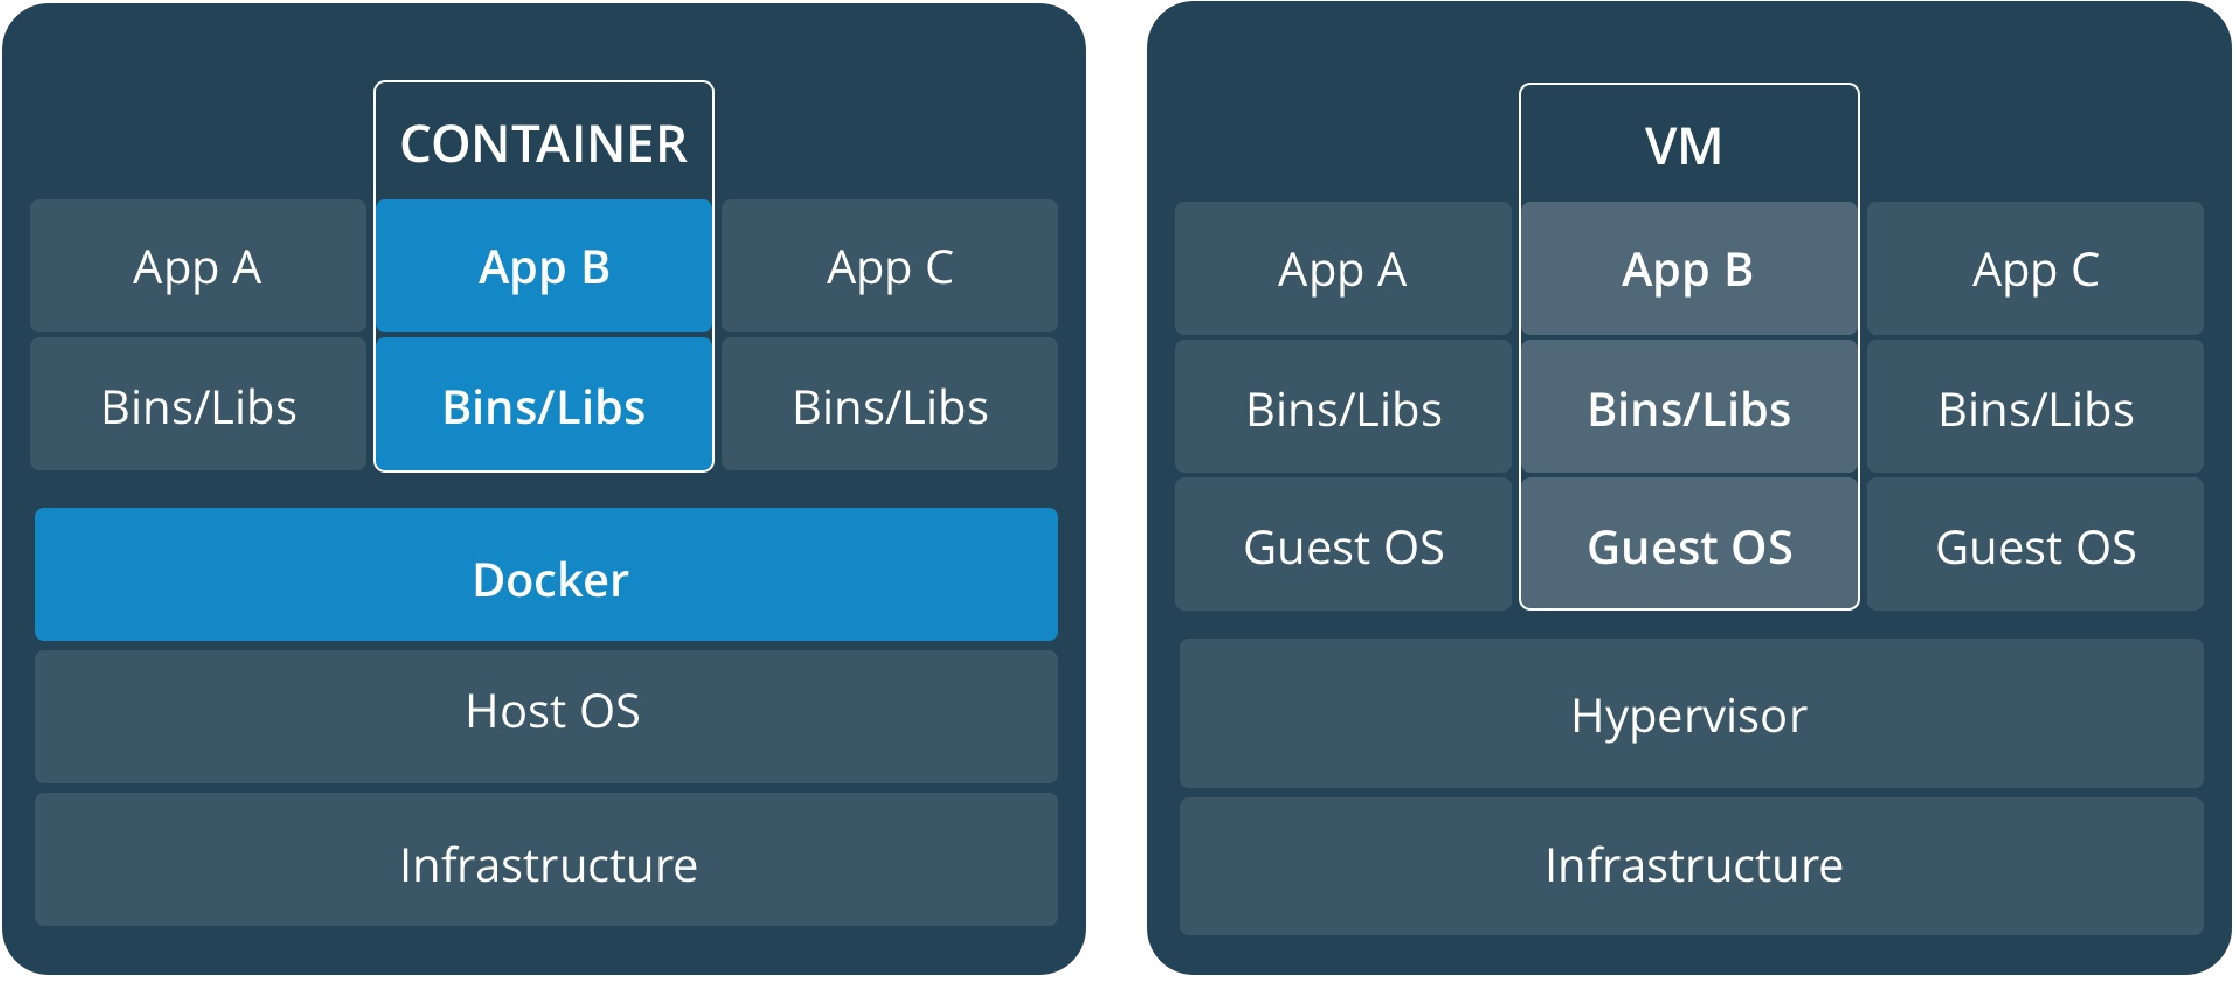
\includegraphics[width=0.8\textwidth]{chapter-background/containervsvm.pdf}
\end{figure}
\subsubsection{Docker}
Recently, thanks to Docker~\cite{dockersite}, containers have gained popularity and have been adopted into the software development process. However, Docker is not a new container technology, at its core it employs the kernel-level mechanisms of Linux containers (LXC), for which it defines a unified API~\cite{merkel2014docker}. In addition, the open-source Docker project offers a commandline-interface and daemon that offers easy packaging of applications in containers and the deployment of these containers.\\\\
To achieve this Docker introduces the concept of images. A container is represented by a lightweight image. A container image is a lightweight, executable package containing an application and its dependencies (runtime, libraries, environment variables, and config files). Virtual machines (VMs) can be seen as full, monolithic images. In particular,  Docker image consists of file-system layers stacked upon each other, as illustrated in Figure~\ref{docker-layers}. Only the top layer, the container itself, is writable, therefore it is state-full and executable. A container is thus composed out of layers of individual images built on top of a base image, allowing for easy extensibility.~\cite{pahl2015containerization} \\\\
A Docker image is specified by and build from a DockerFile. Images can be made easily accessible through Docker registries such as Dockerhub.\\
These images allow for easy and fast deployment of Docker containers across different operating systems and cloud provider stacks. Resulting in a game-changing technology for DevOps, system administrators and developers.
\begin{figure}[H]
\caption{Architecture of a container image. Images can be stacked upon each other using the cgroups and namespace extensions of a Linux kernel. The top container image is writable.~\cite{pahl2015containerization} \label{docker-layers}}
\centering
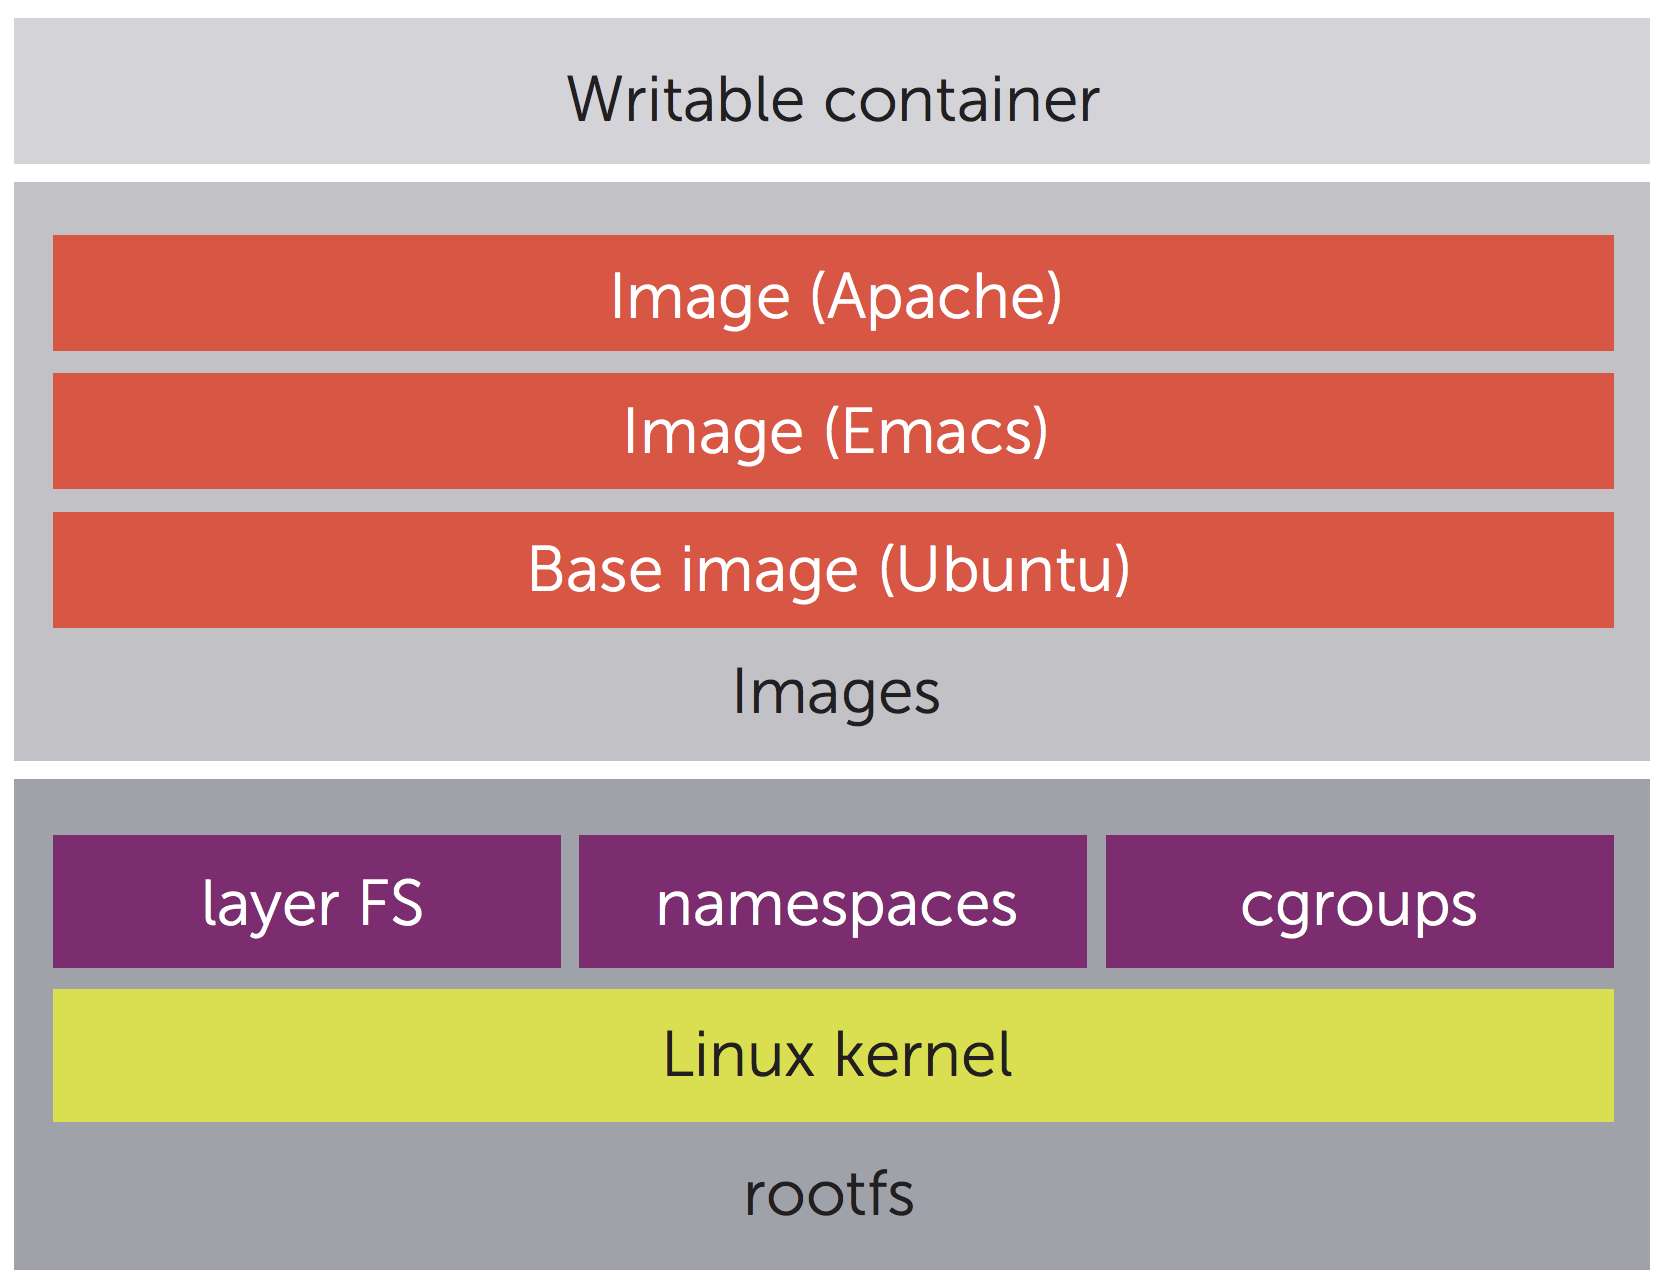
\includegraphics[width=0.5\textwidth]{chapter-background/docker-layers.png}
\end{figure}

\section{Container Orchestration}
Container technologies such as Docker offer advanced features to use containers in production. These solutions often offer deployment of applications limited to single machines. However, applications offered by  SaaS providers may include multiple different containers working together running on a cluster of nodes. Container orchestration (CO) systems allow deployment and management of containers at scale. Popular orchestration engines are Kubernetes, Docker Swarm and Mesos Marathon.
\subsection{Key capabilities of a container orchestration platform}
The task of a container orchestration (CO) platform is not limited to the initial deployment but the entire life-cycle of multiple containers. The goal of CO is to simplify cluster management while ensuring fault tolerance, availability, scalability and reliability. Allowing users to benefit from the complete potential of containers. In order to meet this goal, CO platform must at least offer the following key capabilities.~\cite{khan2017key}
\paragraph{Cluster state management and scheduling}
A cluster can be composed out of multiple virtualized or physical instances. Running containers on top of these instances and recover from failures requires a stable cluster. State management encapsulates various tasks such as flexible scheduling, re-partitioning of resources and data and propagating of dependent system changes.~\cite{khan2017key} 
\paragraph{High availability and fault tolerance}
A container orchestration platform must ensure high availability and fault tolerance in order to be useful for application developers. Most platforms therefor employ design principles of reliability engineering e.g., single point of failure elimination, failure detection or load balancing.~\cite{khan2017key}
\paragraph{Security}
Containers executing on top of the platform essentially form untrusted entities, with potentially malicious intentions, a high security standard is required. The standard should include: container images sanity check policies, access control for both containers and users, and techniques to minimize the container attack surface.~\cite{khan2017key}  
\paragraph{Simplified networking}
Containers must be able to communicate across nodes in  an efficient and secure manner. This requires the mapping of allocated host ports to containers. The overhead corresponding to this mapping intensifies at scale. The CO platform should thus provide a flexible, secure and scalable solution for networking.~\cite{khan2017key}
\paragraph{Service discovery}
The large number of services present in a cluster need to be able to communicate with each other. In traditional clusters services were handled as pets (i.e, having static names, IP addresses), however, in dynamic environments such as container orchestration platforms, they are regarded as cattle. The CO platform must provide mechanisms for addressing/labeling/grouping and service discovery.~\cite{khan2017key} 
\paragraph{Monitoring and governance}
The container orchestration platform needs to support traditional monitoring techniques such as logging, resource usage and network trace-routes. Monitoring must be possible at both the level of the underlying infrastructure and the containers themselves.~\cite{khan2017key}
\paragraph{Integrating for continuous integration and delivery}
Software development teams should be able to integrate the CO platform within their employed continuous integration and delivery (CI/CD) pipeline. The CO platform should contain mechanisms for rolling updates, rollbacks, etc.~\cite{khan2017key}


\subsection{Kubernetes}
Kubernetes~\cite{kubernetes}, commonly referred to as K8,  is one of the most popular and adopted orchestration systems. It is an open-source project led by Google. Kubernetes is Google's solution for the growing demand of container deployments by external developers in its public business cloud and is based upon its predecessors  Borg~\cite{verma2015large} and Omega~\cite{schwarzkopf2013omega} that have been used to schedule the internal Google workload. Its main design goal is formulated as:\textit{ "to make it easy to deploy and manage complex distributed systems, while still benefiting from the improved utilization that containers enable~\cite{Burns:2016:BOK:2930840.2890784}"}.  \\\\
\noindent To achieve the above stated goal Kubernetes introduces a number of concepts for both containers and cluster resources. It implements the infrastructure as code model  by provides an abstraction layer on top of the physical infrastructure~\cite{hermanns2015current}. It allows to setup and manage container infrastructure by the configuration of these introduced concepts via a REST API or declarative YAML configuration files. Below the most relevant concepts are introduced.
\subsubsection{Kubernetes concepts}
\textbf{Pods.}  A pod is the smallest unit of deployment within Kubernetes. It is a group of one or more containers that logically belong together.   A pod and thus its containers run on the same node. They share the same network, storage and context (Linux namespaces, cgroups). A pod gets assigned a unique IP address. Pods are not self-healing meaning when an error occurs within the pod or during scheduling. It will be deleted. Due to this short life cycle using a single pod resource and its assigned IP address for applications is impractical. Kubernetes handles this by employing controllers and services.~\cite{pods}\\\\
\textbf{Deployments.}  A Deployment controller manages a pod or a ReplicaSet of pods. A ReplicaSet allows pods to be replicated across multiple nodes. A Deployment object is used to specify the desired state of pods (e.g. number of replica's). A deployment, in addition, allows for declarative updates. These updates can be used to change the number of container replicas of a ReplicaSet or to update a specific container image within the pod.  The Deployment controller changes the actual state to the desired state described by the update.~\cite{deployments}
\\\\
\textbf{Services.}  Services offer a solution for the short life cycle of pods (and their IP addresses). Services within Kubernetes offer a manner to expose a ReplicaSet of Pods via a unique name, stable IP address, network policy and ports. To determine which set of pods is targeted by a service, Kubernetes employs a Label selector. Labels are the core grouping primitive of Kubernetes and unlike names and UIDs do not offer uniqueness.\\  A Service can be exposed outside the cluster by using an external load balancer or by specifying a NodePort. When using a Nodeport each node within the cluster will expose the port and forward request into the service.~\cite{services}
\\\\
\textbf{Namespaces.}  Namespaces allow to partition resources of a physical cluster among multiple user organizations. Each namespace gets a share of the resources of the cluster, via resource quotas. Resource quotas are supported for CPU, memory and persistent volumes.~\cite{namespaces-k8}
\\\\
\textbf{Resource limits.}  Kubernetes allows the allocation of compute resources of both containers and Namespaces by the means of resource limits. These limits can be soft (limit) and hard (request) limits. A Request specifies the quantity of resource that is guaranteed to the container. A limit specifies the maximum quantity allocated to the container. When the requested resource quantities of a container are less than its limit, the container may be allocated additional resources if there are unallocated resources available.  The current supported compute resources are CPU, memory and storage within the root partition of the local node. Within a Pod it is possible to specify both request and limit for each container. When request and limits are specified, the scheduler will use them for both scheduling and eviction (when node capacity is reached) decisions.~\cite{kubresources}
\subsubsection{Kubernetes architecture}
The basic architecture of Kubernetes is illustrated in Figure~\ref{fig:kubarch}. A client-server architecture is employed in which master and node setups are deployed on different machines. Below the different components that build up the architecture are briefly explained. 
\paragraph{API Server.} The API server is responsible for the configuration and validation of API objects (pods, deployments, services,...). It offers communication on cluster state via a REST interface for both components and administrators.~\cite{kubernetes-api-server}
\paragraph{Controller manager.} The controller manager is responsible for managing several core control loops part of Kubernetes. A control loop uses the API server to observe the shared state of the cluster and attempts to move to the desired state via configuration changes.~\cite{kubernetes-controller-manager}
\paragraph{Scheduler.} The task of assigning pods to nodes is the responsibility of the scheduler component.  The scheduler attempts to do a reasonable placement based on resource and quality of service requirements (e.g., not place a pod on a node with insufficient resources). It is  possible for users to control the placement of pods via NodeSelector tags or affinity and anti-affinity constraints in the configuration file.~\cite{kubernetes-pods-to-nodes,kubernetes-scheduler}
\\\\In addition it is possible to assign Quality of Service (QoS) classes to pods. These are used by Kubernetes in the decision process about scheduling and eviction of pods. Currently, Kubernetes supports three types of classes: guaranteed, burstable and best-effort. In decreasing order of priority (i.e., most likely to be killed in the case of resource shortages). The QoS classes are assigned to pods based on the presence of request and limit specifications of resources in their configuration files.~\cite{kubernetes-qos}


\paragraph{Kubelet.} The kubelet component is an agent running on each node. It is responsible for running and maintaining pods on its residing node. The set of maintained pods is described in the form of PodSpecs (mainly received via the API-server).~\cite{kubernetes-kubelet}
\paragraph{Kube-proxy.} The kube-proxy daemon provides a simple network proxy for the services on each node. It enables forwarding of requests to the correct containers and can provide primitive load balancing.~\cite{kubernetes-kubeproxy}
\begin{figure}[H]
\caption{Kubernetes architecture}
\centering
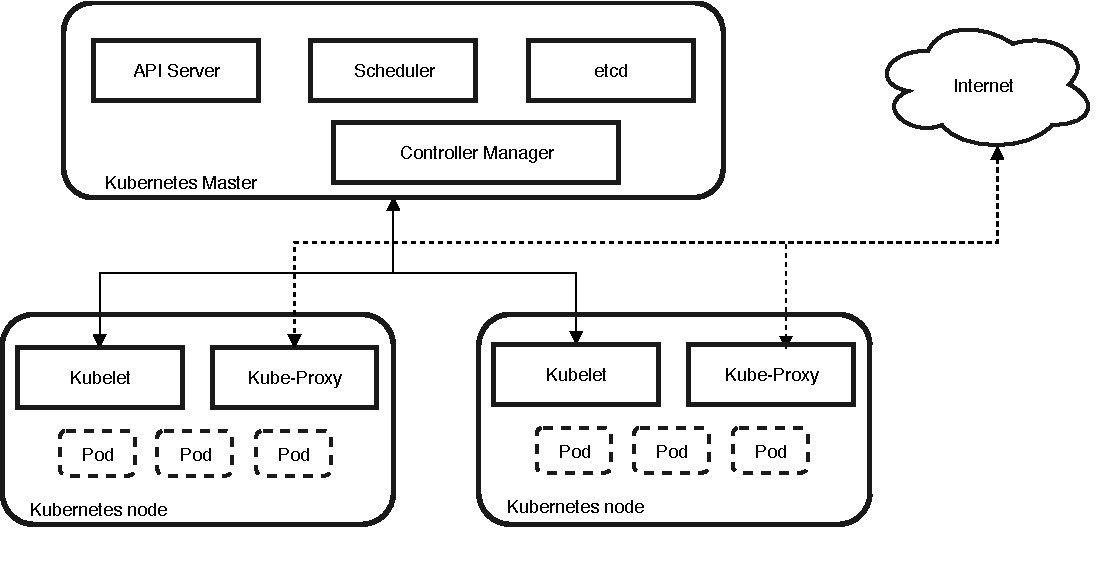
\includegraphics[width=0.8\textwidth]{chapter-background/kubernetes-architecture-diagram.pdf}
\label{fig:kubarch}
\end{figure}
 
 
 
 
 
 
 
 
 
 \section{Performance evaluation}
As discussed in previous sections, SaaS providers employ multi-tenancy to improve  cost efficiency and offer several performance guarantees to their customers in the form of SLOs. An unavoidable consequence of multi-tenancy is the need to support a growing number of users in a single system. Providers need to have a clear insight into the \textit{scalability} of their systems. However, scalability is a difficult thing to define, let alone quantify. Citing the words of  Dr. Neil J. Gunther:  \textit{"if you can't quantify it, you can't guarantee it"}.~\cite{perfdynamics}

\subsection{The Universal Scalability Law}
\label{section-USL}
Dr. Neil J. Gunther provides a formal definition of scalability: \textit{"scalability can be defined as a mathematical function, a relationship between independent and dependent variables (input and output)"~\cite{perfdynamics}}. The Universal Scalability Law (USL) by Dr. Neil J. Gunther is presented in Equation~\ref{USL}. It computes the relative capacity $C(N)$ at a load of $N$ users. Relative capacity is the normalized throughput.
\begin{equation}
\label{USL}
C(N) = \frac{\gamma~N}{1 + \alpha~(N-1) + \beta~N~(N-1)}
\end{equation}

The Universal Scalability Law incorporates factors that contribute to the sublinearly scalability of most systems. Namely, \textbf{concurrency} ($\gamma$), \textbf{contention} ($\alpha$) and \textbf{coherency} ($\beta$) as explained below. Their impact is visualized in Figure~\ref{fig:usl-impact}.

\begin{itemize}
    \item \textbf{Concurrency}($\gamma$): $\gamma$ defines the slope if the system was linearly scaling i.e., $C(N) = \gamma N$. It has been referred to as the \textit{coefficient of performance} by~\cite{schwarz2015practical}.
    \item \textbf{Contention} ($ \alpha $) : When scaling most systems parallelism while be limited at some point by contention (i.e., waiting or queuing for shared resources). The maximum speedup by parallelism is limited by the serialized portion ($\alpha$) of the work~\cite{schwarz2015practical}. 
    \item \textbf{Coherency} ($\beta$): created by crosstalk between components. Because crosstalk is possible between each pair of components in the system, the penalty grows quadratic $N(N-1)$.~\cite{schwarz2015practical}
    
\end{itemize}

\begin{figure}
    \centering
    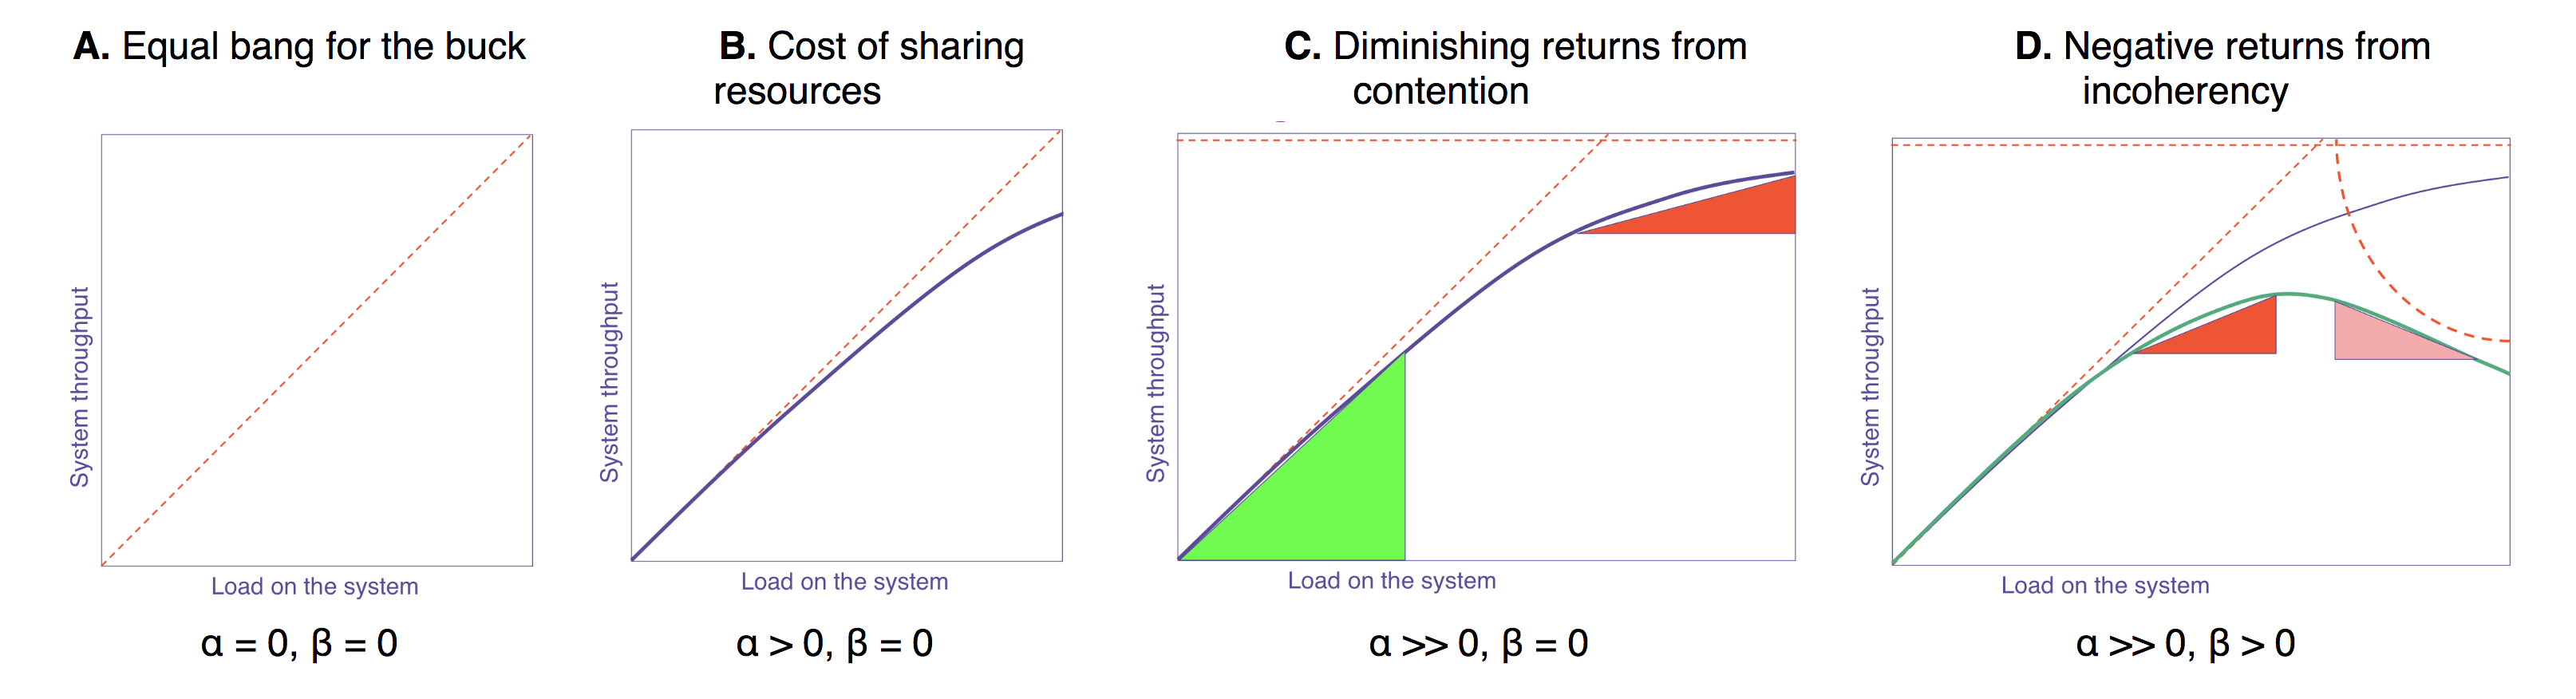
\includegraphics[width=1.1\textwidth]{chapter-evaluation/usl-impact}
    \caption{The impact of different USL coefficients on scalability.~\cite{perfdynamics}}
    \label{fig:usl-impact}
\end{figure}

\subsubsection{USL in practice}
USL can provide insights into a system's scalability pains via  values of the concurrency, contention and coherency coefficients. These can be obtained by collecting a dataset of measurements of the system, system load $N$ and corresponding throughput, and using a statistical technique such as nonlinear least square regression which fits the USL to the dataset.~\cite{schwarz2015practical,heyman2014scalability}

\subsection{Little's law}
\label{sec:little}
The Universal Law of Scalability serves as an alternative for the often less intuitive queuing models frequently used for modeling scalability. It omits the need to know the service time for every queue in the performance model in order to predict the response time or latency~\cite{perfdynamics}. Nevertheless, queuing theorem and its lemmas such as Little's Law can provide useful insights into performance modeling.\\\\
John D.C Little's Law~\cite{little2008little} states the following for stable systems: 
\begin{displayquote}
\textit{"The average number of items in a queuing system equals the average rate at which items arrive multiplied by the average time that an item spends in the system.\cite{little2008little}"}
\end{displayquote}
\begin{equation}
\label{littleslaw}
L = \lambda~W
\end{equation}
\begin{equation}
\label{llsys}
N = X~Rt
\end{equation}
Equation~\ref{littleslaw} shows Little's law, below its terms and its applicability to web services (Equation~\ref{llsys}) are explained:
\begin{itemize}
    \item \textbf{$L$}:  Average number of items in the system. For a web service this is represented by the average number of concurrent users in the system $N$.
    \item \textbf{$\lambda$}: Long-term average arrival rate of items in the system per time unit. Little's law assumes a stable system for which the arrival rate and exit rate are identical. In a web service this is represented by the throughput $X$.
    \item \textbf{$W$}: Average waiting time of an item in the system, queuing time and service time combined. This is represented by the response time $Rt$ or latency of a request in a web service. When dealing with a system involving think time (e.g., after the response from a web service, a user needs time to think about his/her next request), $(Rt + Zt)$ is used. 
\end{itemize}

\subsubsection{Workload generator validation}
Developers employ software tools (JMeter~\cite{jmeter}, Locust~\cite{locust}, etc.)  to simulate a workload and test the performance of a system. A workload is a set of actions that represent the behavior of a client in the system. It is part of the test plan stating the number of concurrent users $N$ executing the workload for a specified period of time.\\\\
The results of a performance test are typically expressed in throughput $X$ and response time $Rt$. Using Little's law it is possible to validate these results. For example, a test plan of 1000 concurrent users $N$ results in a throughput of 50 requests per second and an average response time of 15 seconds. Following Little's law, a concurrence of only 750 users was reached, instead of the specified 1000. Little's law can thus be used to check if a workload generator works as specified.\\\\
Alternatively, if the average throughput and response time for a production system are known, Little's law can be used to correctly draw up a test plan.

\subsubsection{Response time or latency?}
Performance can either be measured in throughput or latency, both are correct but offer a different point of view. System performance is typically expressed in throughput: "The system can handle a million operations per second". However, users care more about their personal experience with a system which is influenced by the average latency of their request.~\cite{schwarz2015practical} \\\\
Figure~\ref{fig:ls_vs_tp} shows the relation between the average latency and throughput of a database under increasing load $N$. In this case, latency is kept stable by increasing the throughput with the increasing load up to a certain point.  A bottleneck caps the throughput of the systems and by Little's law for an increasing load and constant throughput, the latency must increase.~\cite{latvsthrough} \\\\
However in other systems, as discussed in Section~\ref{section-USL}, an increasing load might induce a diminishing result on the system's throughput. Following Little's law a decreasing throughput results in a higher latency under the same load. \\\\
Thus, for stable systems by Little's law,  the USL can be reformulated in terms of latency instead of throughput. Equation~\ref{USL-2} shows this reformulation.~\cite{schwarz2015practical}
\begin{equation}
\label{USL-2}
Latency(N) = \frac{1 + \alpha~(N-1) + \beta~N~(N-1)}{\gamma}
\end{equation}


\begin{figure}[H]
    \centering
    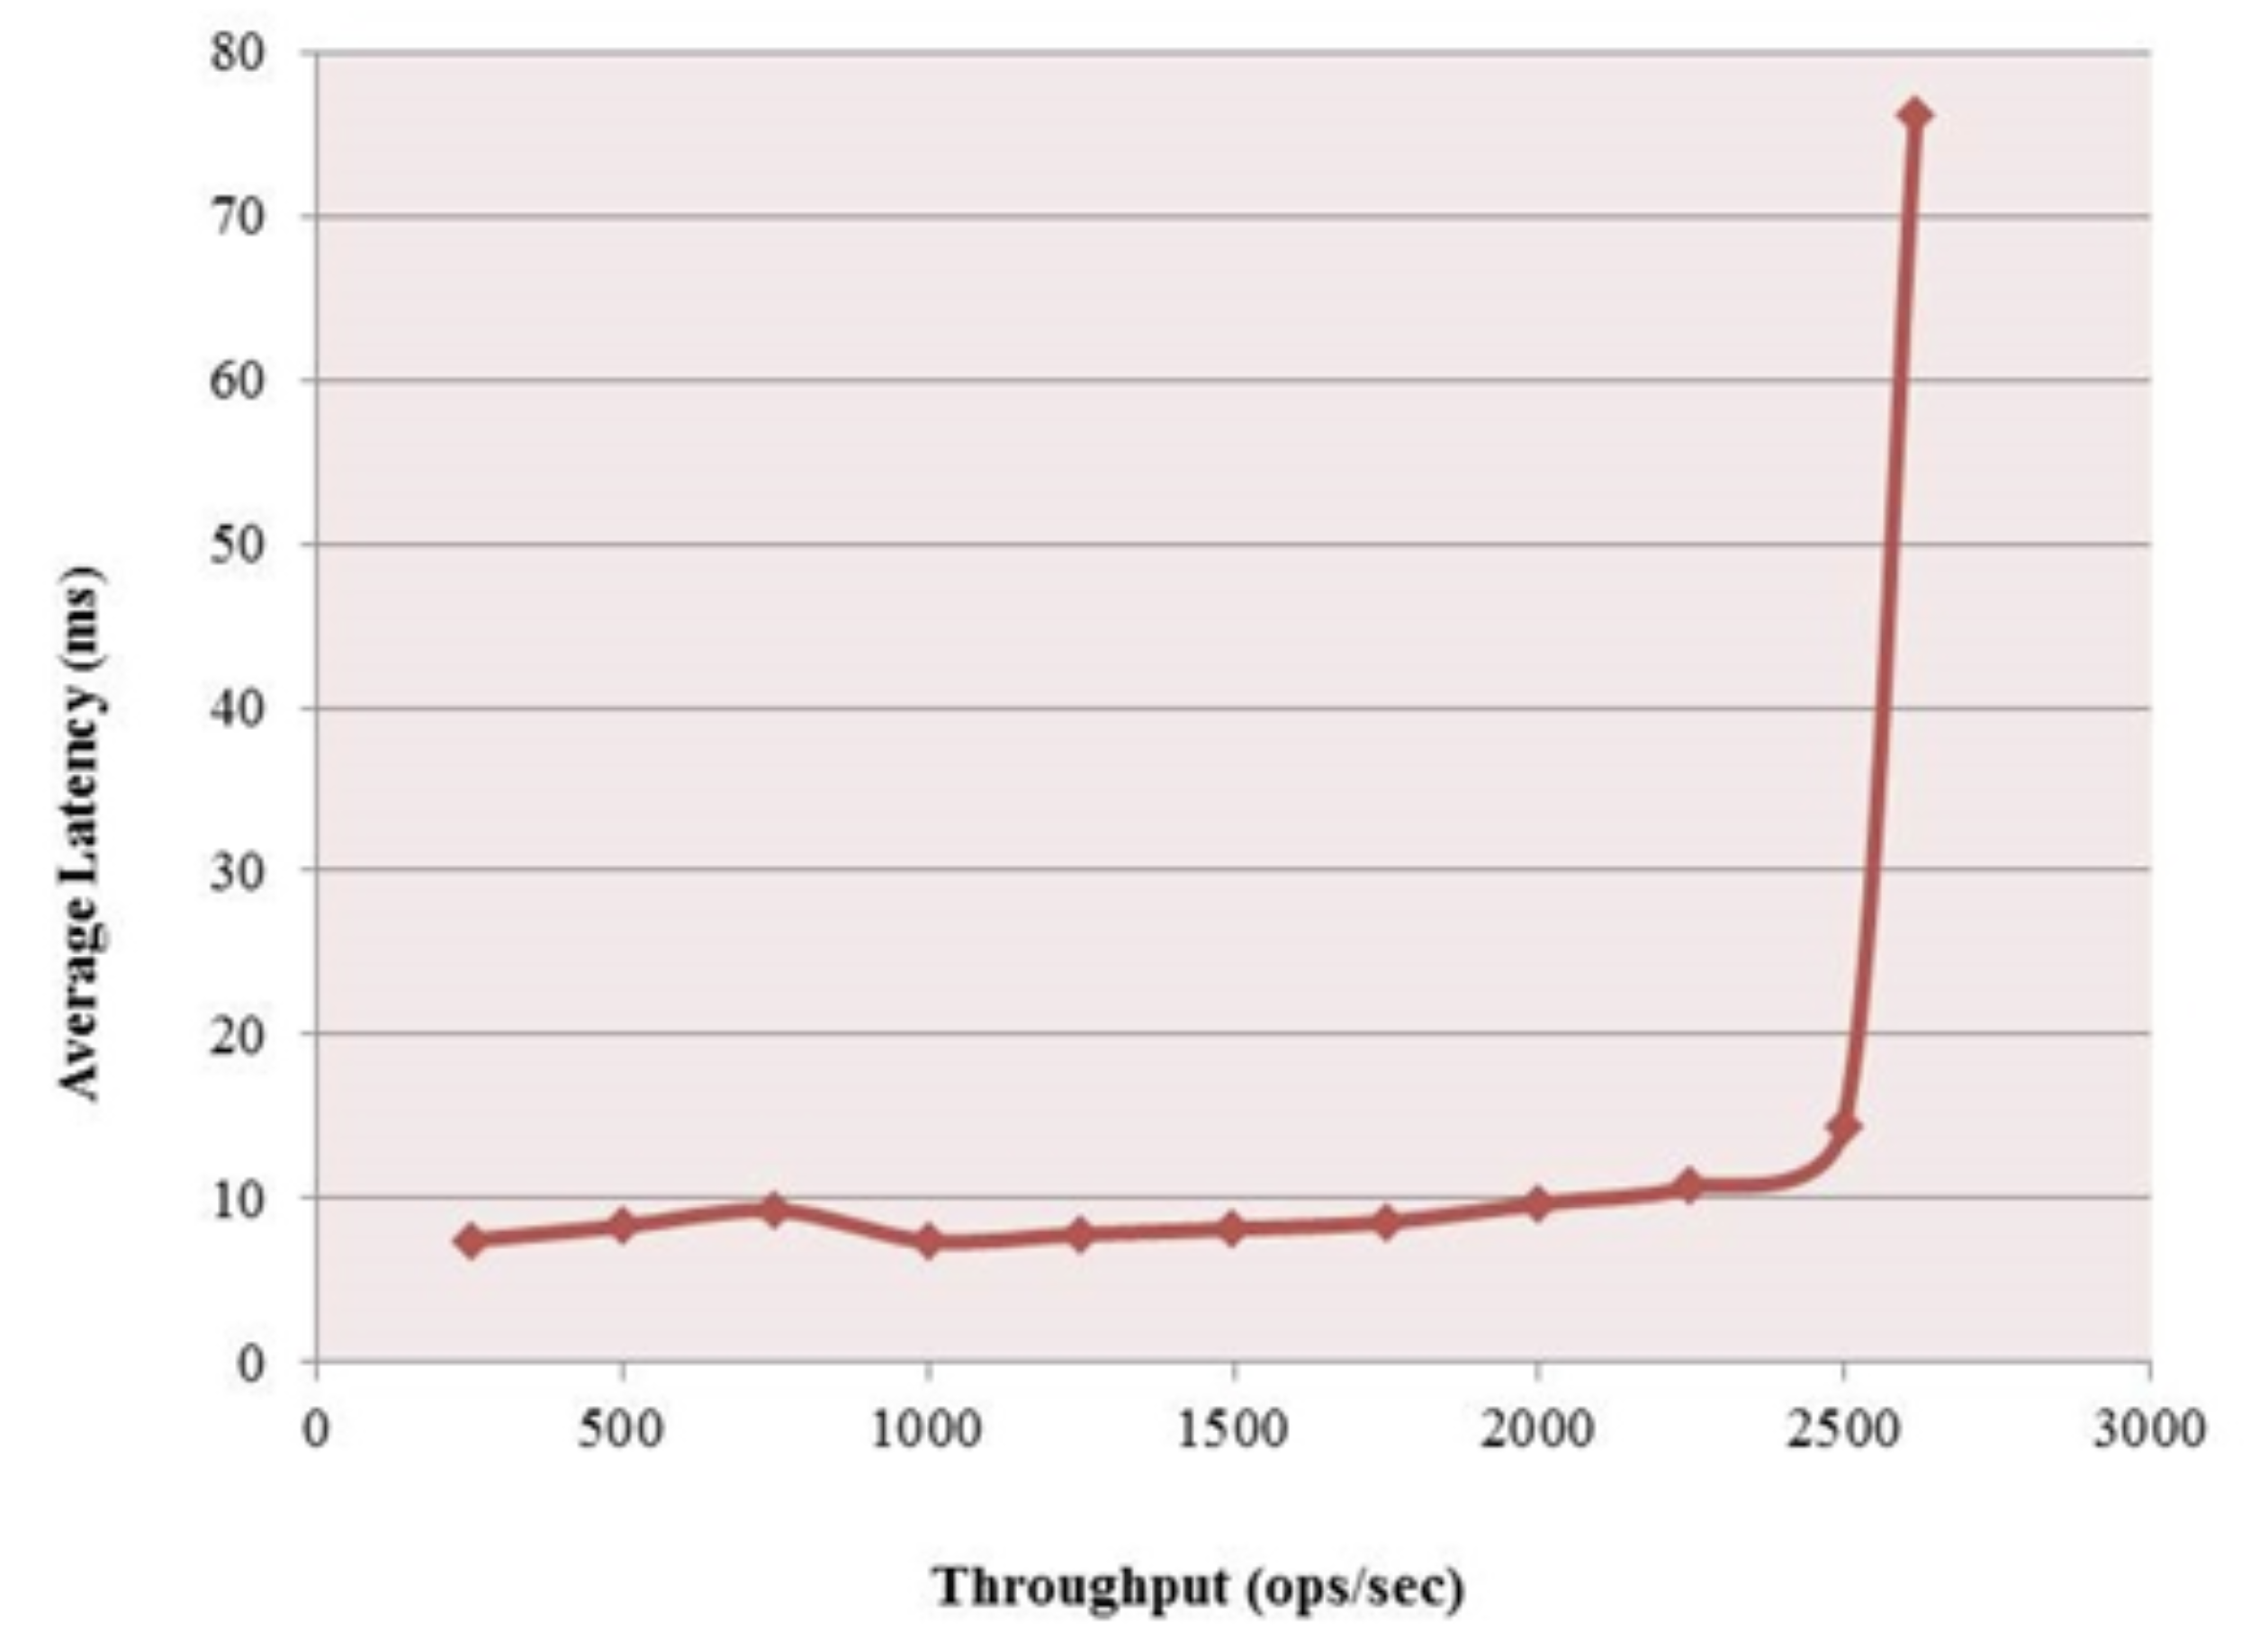
\includegraphics[width=0.8\textwidth]{chapter-evaluation/ls_vs_th}
    \caption{Relation average latency vs. throughput for database benchmark with increasing load.~\cite{latvsthrough}}
    \label{fig:ls_vs_tp}
\end{figure}
% ... and so on until
%\chapter{The Last Appendix}
\label{app:n}
Appendices are numbered with letters, but the sections and subsections use
arabic numerals, as can be seen below.

\section{Lorem 20-24}
\lipsum[20-24]

\section{Lorem 25-27}
\lipsum[25-27]

%%% Local Variables: 
%%% mode: latex
%%% TeX-master: "thesis"
%%% End: 


\backmatter
% The bibliography comes after the appendices.
% You can replace the standard "abbrv" bibliography style by another one.
\bibliographystyle{abbrv}
\bibliography{references}

\end{document}

%%% Local Variables: 
%%% mode: latex
%%% TeX-master: t
%%% End: 
